% **************************************************************************************************************
% A Classic Thesis Style
% An Homage to The Elements of Typographic Style
%
% Copyright (C) 2011 Andr\'e Miede http://www.miede.de
%
% If you like the style then I would appreciate a postcard. My address 
% can be found in the file ClassicThesis.pdf. A collection of the 
% postcards I received so far is available online at 
% http://postcards.miede.de
%
% License:
% This program is free software; you can redistribute it and/or modify
% it under the terms of the GNU General Public License as published by
% the Free Software Foundation; either version 2 of the License, or
% (at your option) any later version.
%
% This program is distributed in the hope that it will be useful,
% but WITHOUT ANY WARRANTY; without even the implied warranty of
% MERCHANTABILITY or FITNESS FOR A PARTICULAR PURPOSE.  See the
% GNU General Public License for more details.
%
% You should have received a copy of the GNU General Public License
% along with this program; see the file COPYING.  If not, write to
% the Free Software Foundation, Inc., 59 Temple Place - Suite 330,
% Boston, MA 02111-1307, USA.
%
% **************************************************************************************************************
% Note:
%    * You must not use "u etc. in strings/commands that will be spaced out (use \"u or real umlauts instead)
%    * New enumeration (small caps): \begin{aenumerate} \end{aenumerate}
%    * For margin notes: \marginpar or \graffito{}
%    * Do not use bold fonts in this style, it is designed around them
%    * Use tables as in the examples
%    * See classicthesis-preamble.sty for useful commands
% **************************************************************************************************************
% To Do:
%		 * [high] Check this out: http://www.golatex.de/koma-script-warnung-in-verbindung-mit-listings-package-t2058.html
%    * [medium] mathbb in section-titles/chapter-titles => disappears somehow in headlines!!!
% **************************************************************************************************************
\PassOptionsToPackage{table,x11names}{xcolor}
% \PassOptionsToPackage{spanish}{babel}
\documentclass[twoside,openright,titlepage,numbers=noenddot,headinclude,%1headlines,% letterpaper a4paper
                footinclude=true,cleardoublepage=empty,abstractoff, % <--- obsolete, remove (todo)
                BCOR=5mm,paper=a4,fontsize=11pt,%11pt,a4paper,%
                ngerman,american%
                ]{scrreprt}

%********************************************************************
% Note: Make all your adjustments in here
%*******************************************************
\usepackage[backref]{classicthesis-preamble}

%*******************************************************
% Some font experiments
%*******************************************************
% \usepackage[osf]{libertine}
%  \usepackage{hfoldsty}
%   \usepackage[light,condensed,math]{iwona}
% \renewcommand{\sfdefault}{iwona}
% \usepackage{lmodern} % <-- no osf support :-(
%  \usepackage[urw-garamond]{mathdesign} %<-- no osf support :-(
%   \usepackage{anttor}
% \usepackage{ccfonts}

% \usepackage{fouriernc}
%   \usepackage{pxfonts}
%  \usepackage{antpolt}
% \usepackage{mbtimes}
% \usepackage[QX]{fontenc}
%  \usepackage{amsmath}
% \usepackage[T1]{fontenc}
% \usepackage[bitstream-charter]{mathdesign}
% \usepackage{condmath}
%   \usepackage{fouriernc}
% \usepackage{kerkis}
% \usepackage{millennial} %millennial.sty not found
  \usepackage{fourier}
%  \usepackage{kurier}
%  \usepackage{mathpazo}
% \usepackage{mathpple}
%\usepackage{mathptmx} %esta
 %\usepackage{euler}
% \usepackage[utopia]{mathdesign}
% \usepackage[charter]{mathdesign}
%  \usepackage[varg]{txfonts}
% \usepackage{txfonts}
% \usepackage{arev}
% \usepackage{cmbright}
% \usepackage{kmath}
%\usepackage{mathptmx}

%=========================
% Algunos paquetes
%=========================
\usepackage{makeidx}
\usepackage{amssymb,bm}

\usepackage{natbib}
%\usepackage[authoryear,round,colon]{natbib}

\usepackage{environ}
\usepackage{ifthen}
\usepackage{enumitem}
%\usepackage{slashbox}
\usepackage{anyfontsize}
\usepackage{hyperref}
%\usepackage[total={10cm,10cm},top=2cm, left=2cm]{geometry}
\usepackage{lscape}

\usepackage{leftidx}

\usepackage{relsize}

\usepackage{listings}             % Include the listings-package

%\usepackage{siunitx}

% \usepackage{graphicx}
% \usepackage{caption}
% \usepackage{subcaption}
 

%=================
% Un paquete Grafico
%=================
\usepackage{boiboites}
\newboxedtheorem[boxcolor=Blue, background=blue!5, titlebackground=blue!20,titleboxcolor = black]{theo}{}{}


%SETUP Hyper=====================================================================================================================
\hypersetup{colorlinks=true}
\hypersetup{urlcolor=halfgray}
 %\hypersetup{linkcolor=blue}
 %\hypersetup{citecolor=red}
% \hypersetup{linkbordercolor=white}
%================================================================================================================================


%=================
% Graficos Especiales
%==================
\usepackage{tikz}
\usetikzlibrary{shapes,snakes}
% Tabla
\usetikzlibrary{calc}
\pgfdeclarelayer{background}
\pgfdeclarelayer{foreground}
\pgfsetlayers{background,main,foreground}


%\usepackage[pdftex]{graphicx} % PDFLaTeX
%\DeclareGraphicsExtensions{.png,.pdf,.jpg}
%\usepackage[x11names]{xcolor}


% \usepackage[spanish]{babel}




%*****************************
%    MIS COMANDOS
%*****************************
% \newcommand{\I}{\noindent}
% \newcommand{\DTdt}[1]{\frac{d^2{#1}}{dt^2}}
% \newcommand{\DFdt}[1]{\frac{d{#1}}{dt}}
% \newcommand{\DdFdt}[1]{\dfrac{d{#1}}{dt}}
% \newcommand{\Pt}[1]{\overset{\centerdot}{#1}}
% \newcommand{\PPt}[1]{\overset{\centerdot\centerdot}{#1}}
% \newcommand{\vel}[1]{\mathbf{\Pt{#1}}}
% \newcommand{\acel}[1]{\mathbf{\PPt{#1}}}
% \newcommand{\cruz}[2]{\mathbf{#1}\times\mathbf{#2}}
% \newcommand{\cruzT}[2]{{#1}\times{#2}}
% \newcommand{\point}[2]{\mathbf{#1}\cdot\mathbf{#2}}
% \newcommand{\blue}[1]{\textcolor{blue}{#1}}
% \newcommand{\red}[1]{\textcolor{red}{#1}}
% \newcommand{\white}[1]{\textcolor{white}{#1}}
% \newcommand{\White}{\color{white}}
% \newcommand{\Dpartial}[1]{\frac{\partial{#1}}{\partial t}}
% \newcommand{\DTpartial}[1]{\frac{\partial^2{#1}}{\partial t^2}}
% \newcommand{\Partial}[2]{\frac{\partial{#1}}{\partial {#2}}}
% \newcommand{\TPartial}[2]{\frac{\partial^2{#1}}{\partial {#2}^2}}
% \newcommand{\bs}[1]{\boldsymbol{#1}}
% \newcommand{\w}{\omega}
% \newcommand{\unit}[1]{\mathbf{\hat{{#1}}}}
% \newcommand{\cor}[1]{\left[ #1\right]}
% \newcommand{\pr}[1]{\left( #1\right)}
% \newcommand{\rd}{\mathrm{d}}
% \newcommand{\hs}[1]{\hspace{#1}}
% \newcommand{\vs}[1]{\vspace{#1}}
% \newcommand{\Deg}{\text{\textdegree}\;}
%#####################################
% \newcommand{\enum}[1]{\begin{enumerate} #1  \end{enumerate}}
% \newcommand{\sizeF}[2]{\fontsize{#1}{#1}\selectfont #2}
% \newcommand{\spS}[1]{\quad #1 \quad}
% \newcommand{\spD}[1]{\quad #1 \quad}
% \newcommand{\mbf}[1]{\mathbf{#1}}
%####################################
\renewcommand\thefootnote{\textcolor{halfgray}{\arabic{footnote}}} % Poniendole color al footnote}
%\renewcommand{\figurename}{Figura}
%\renewcommand*{\contentsname}{Contenido}
% \newcommand{\adg}{$a\dagger$}


% \tikzstyle{mybox} = [draw=blue, fill=blue!10, very thick,
%     rectangle, rounded corners, inner sep=10pt, inner ysep=20pt]
% \tikzstyle{fancytitle} =[fill=blue!30, text=black]


%=========================
% MY ENVIROMENTS
%=========================
\NewEnviron{BOX}[2]{%
      \tikzstyle{mybox} = [draw=blue, fill=blue!5, very thick, rectangle, rounded corners, inner sep=10pt, inner ysep=20pt]
      \tikzstyle{fancytitle} =[fill=red, text=white]
      \begin{tikzpicture}
      \node [mybox] (box){%
	  \begin{minipage}{#1\textwidth}
	  \textit{\BODY}
	  \end{minipage}
      };
      \ifthenelse{\equal{#2}{}}{Blank}{\node[fancytitle, right=10pt,rounded corners] at (box.north west) {#2};}
%       \newif\ifTitle
%       \Titletrue
% 	\ifTitle{
% 	\node[fancytitle, right=10pt,rounded corners] at (box.north west) {#2};
% 	\node[fancytitle, rounded corners] at (box.east) {$\clubsuit$};}
% 	\else
% 	%
% 	\fi
      \end{tikzpicture}%
}

 %*******************
 % listas con puntos
 %*******************
 \RequirePackage{enumitem}
 \newcommand*{\itembolasgrises}[1]{%
 \footnotesize\protect\tikz[baseline=-3pt]%
 \protect\node[fill=gray!50,shape=circle,draw,inner sep=1.2pt,line width=0.2mm](n1){#1};}
 \newcommand*{\itembolasazules}[1]{%
 \footnotesize\protect\tikz[baseline=-3pt]%
 \protect\node[scale=.2, circle, shade, ball color=blue]  {\color{white}{\fontsize{50pt}{50pt}\selectfont\bf#1}};}
 \newcommand*{\itembolasverdes}[1]{%
 \footnotesize\protect\tikz[baseline=-3pt]%
 \protect\node[scale=.2, circle, shade, ball color=green]  {\color{white}fontsize{50pt}{50pt} \selectfont\bf#1};}
 \newcommand*{\itembolasrojas}[1]{%
  \footnotesize\protect\tikz[baseline=-3pt]%
  \protect\node[scale=.2, circle, shade, ball color=red]  {\color{white}fontsize{50pt}{50pt} \selectfont\bf#1};}



%*******************************************************
% Fine-tuning for the text area
%*******************************************************
% Margenes anteriores 
% \linespread{1.05} % a bit more for Palatino
% \areaset[current]{312pt}{761pt} % 686 (factor 2.2) + 33 head + 42 head \the\footskip
% \areaset[current]{350pt}{760pt}
% \setlength{\marginparwidth}{7em}%
% \setlength{\marginparsep}{2em}%

\linespread{1.05} % a bit more for Palatino
% \areaset[current]{312pt}{761pt} % 686 (factor 2.2) + 33 head + 42 head \the\footskip
\areaset[current]{430pt}{760pt}
\setlength{\marginparwidth}{8.5em}%
\setlength{\marginparsep}{2em}%

%********************************************************************
% Hyphenation
%*******************************************************
%\hyphenation{put special hyphenation here}
%\brokenpenalty=10000    %Desabilita los saltos de lineas y de pagina
%\hyphenpenalty=10000
\pretolerance=2000
\tolerance=3000

% ********************************************************************
% GO!GO!GO! MOVE IT!
%*******************************************************
\makeindex  %esto es para crear el INDICE ALFABETICO


\begin{document}
\frenchspacing
\raggedbottom
%\selectlanguage{spanish}
\selectlanguage{american} % american ngerman

%\renewcommand*{\bibname}{new name}
%\setbibpreamble{}
\pagenumbering{roman}
\pagestyle{plain}
%********************************************************************
% Frontmatter
%*******************************************************
%\include{FrontBackmatter/DirtyTitlepage}
%*******************************************************
% Titlepage
%*******************************************************
\begin{titlepage}
	% if you want the titlepage to be centered, uncomment and fine-tune the line below (KOMA classes environment)
	\begin{addmargin}[-1cm]{-3cm}
    \begin{center}
        \large  

        \hfill

        \vfill

%		\includegraphics[width=0.3\textwidth]{gfx/Logo_Udea.jpg} \\ \bigskip 
%		%\mySubtitle \\ 
%		\medskip 		
%		\myDepartment \\                            
%        \myFaculty \\
%        \myTime		
		
		
		
		\vspace{1cm}


        \begingroup
            
            \emph{\color{halfgray}\hspace*{0.83cm}{\centering\spacedallcaps {\LARGE {\hspace*{0.4cm}{Searching for exoplanetary rings with \newline 
            \hspace*{0.8cm}{\textit{SuperWASP} and \textit{Gaia} } } } } } }\\ \bigskip
                        
        \endgroup
       
        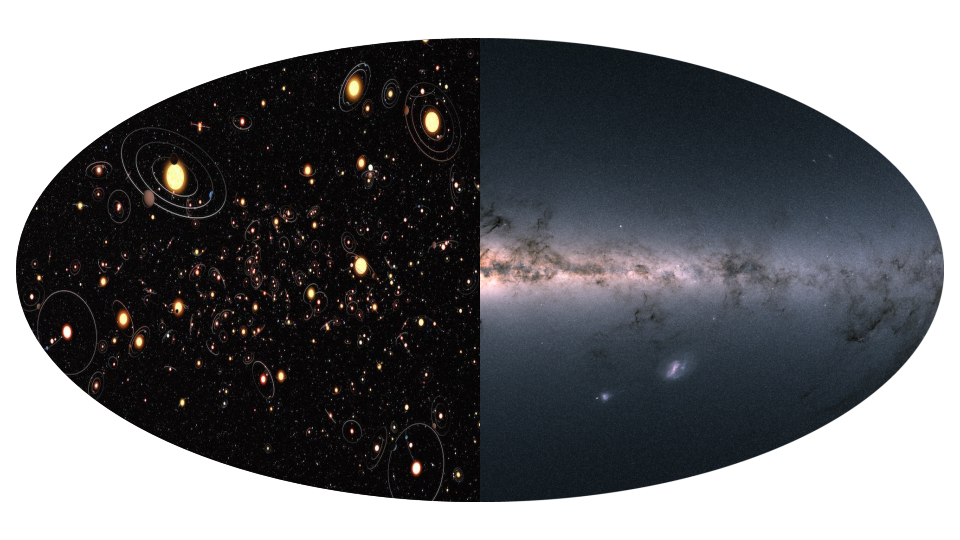
\includegraphics[width=11.5cm,height=6cm]{gfx/EXO_4.png} \\   
        %\includegraphics[width=12cm,height=6cm]{gfx/EXO_3.jpg} \\  
        
		\vspace{0.5cm}
		\medskip
		\small \textbf{MAJOR RESEARCH PROJECT IN ASTRONOMY}\\
		\vspace{1.0cm}
		\textbf{Presented by:}\\
        \spacedlowsmallcaps{\myName}
      

%        \includegraphics[width=0.3\textwidth]{gfx/Logo_Udea.jpg} \\ \bigskip 
		%\mySubtitle \\ 
%		\medskip 		
		
		\vspace{1cm}
        \myDegree \\
        

        \vspace{1cm}
         \textbf{Under the supervision of}\\ \medskip
        \myProf\\ \medskip
         %\textbf{Second Reader}\\ \medskip
        %\myOtherProf\\
        
        \vfill
        \includegraphics[width=0.65\textwidth]{gfx/Logo_Leiden.png} \\ \bigskip 
        \vspace{0.05cm}
        \myDepartment \\                            
        \myFaculty \\
        \myTime
        %\myUni \\ \bigskip

        %\myTime

        \vfill                      

    \end{center}  
  \end{addmargin}       
\end{titlepage}   

\include{FrontBackmatter/Titleback}
 %\cleardoublepage\include{FrontBackmatter/Dedication}
\cleardoublepage%*******************************************************
% Abstract
%*******************************************************
%\renewcommand{\abstractname}{Abstract}
\pdfbookmark[1]{Abstract}{Abstract}
\begingroup
\let\clearpage\relax
\let\cleardoublepage\relax
\let\cleardoublepage\relax

% \chapter*{Abstract}
\chapter*{Abstract}


\vfill
In this work, we present a probabilistic analysis of the occurrence rate of exoplanetary rings. Following a Monte-Carlo and analytic approach to reproduce the stellar mass IMF and the exoplanetary mass-and period-distributions, we proposed low-mass stars below $2.0 \textnormal{M}_\odot$ as those candidates with the highest chance to harbor planets orbiting with exoplanetary rings (already formed or in the formation process). The expected number of detections lies between $100$ and $10$ for a stellar mass range between $0.1 \textnormal{M}_\odot$ and $2.0 \textnormal{M}_\odot$, out of a total number of $10\,000$ stars and exoplanets period-mass pairs simulated. Using \textcolor{halfgray}{\textit{Gaia} DR2} data we performed an analysis of the well-known OB association ScoCen (also known as Sco OB2) subdividing the region in three subgroups, \textcolor{halfgray}{\textit{Upper Scorpius}}, \textcolor{halfgray}{\textit{Upper Centaurus-Lupus}}, and \textcolor{halfgray}{\textit{Lower Centaurus-Crux}}. For each subgroup, its respective Hertzsprung-Russell was created to pre-select stars between two isochrone models of $5 \textnormal{Myr}$ and $60 \textnormal{Myr}$, where the youngest isochrones were corrected by extinction values reported in the literature. Stellar tracks where also computed probing that our final sample contains stars below $2 \textnormal{M}_\odot$ to values down to $0.1 \textnormal{M}_\odot$ which corresponds to the lower limits of the isochrone-and stellar track-models. However, we can go a bit further down this limit in mass with the new \textcolor{halfgray}{\textit{Gaia} DR2} data set. The final sample contains $3\,729$, $3\,309$, and $3\,432$ sources in each one of the \textcolor{halfgray}{LCC}, \textcolor{halfgray}{UCL} and \textcolor{halfgray}{US} subgroups. This final sample of stars is cross-matched to the \textcolor{halfgray}{\textit{SuperWASP}} database in order to retrieve light curves for the selected stars to be studied, motivated by the light curve of J1407. This cross-matching process let us with $113$, $654$, and $718$ light curves per subgroup but only a final sample of $\sim20$ candidates is proposed after inspecting the light curves and comparing to the actual light curve of J1407 searching for possible exoplanetary ringed systems or variable star behavior. Additionally, we redefined the original limits of ScoCen in galactic coordinates to include a larger sky area in a range of $285^\circ\leq\ell\leq360^\circ$ and $-10^\circ\leq b\leq+32^\circ$ and a parallax range of $5$ to $12$ mas and performed a selection of the young population which led to the natural overall trend and some outstanding over-densities close to the original boxes. This method allows the study of membership in associations relatively quick as a first step to lately applied a kinematic method and increase the chance of studying a large sample of actual stars belonging to the association.\medskip \\

Keywords: \textit{planets and satellites: rings --- parallaxes --- techniques: photometric --- open clusters and associations: individual (Sco-Cen)}.

\endgroup			

\vfill
 %\cleardoublepage\include{FrontBackmatter/Publication}
\cleardoublepage%*******************************************************
% Acknowledgments
%*******************************************************
\pdfbookmark[1]{Acknowledgments}{acknowledgments}

\begin{flushright}{\slshape 
    Wat mij betreft weet ik niets zeker,\\
    maar naar de sterren kijken zet me aan het dromen.\\ \medskip}
    ---\color{halfgray}{Vincent Willem van Gogh}\\ \footnotesize\textit{(1853 \texttwelveudash 1890) Dutch Post-Impressionist painter }.
\end{flushright}

\begin{flushright}{\slshape 
    It is sometimes said that scientists are unromantic, \\ that their passion to figure out robs the world of beauty and mystery. \\
    But is it not stirring to understand how the world actually works \texttwelveudash  that white light is made of colors,
    that color is the way we perceive the wavelengths of light,\\ that transparent air reflects light,
    that in so doing it discriminates among the waves, \\ and that the sky is blue for the same reason that the sunset is red? \\
    It does no harm to the romance of the sunset to know a little bit about it.\\ \medskip}
    ---\color{halfgray}{Carl Sagan, Pale Blue Dot: A Vision of the Human Future in Space}\\ \footnotesize\textit{(1935 - 1996) American astronomer, cosmologist, astrophysicist, astrobiologist, author, science popularizer, and science communicator in astronomy and other natural sciences }.
\end{flushright}

\begin{flushright}{\slshape 
    In  third Dialogue there is first denied that base illusion of the shape of the heavens,\\  of their spheres and diversity.\\
    For the heaven is declared to be a single general space,\\ embracing the infinity of worlds,\\ 
    though we do not deny that there are other infinite 'heavens'\\ using that word in another sense.\\ 
    For just as this earth hath her own heaven (which is her own region),\\ through which she moveth and hath her course, \\
    so the same may be said of each of the innumerable other worlds..\\ \medskip}
---\color{halfgray}{Giordano Bruno}\\ \footnotesize\textit{(1548 \texttwelveudash 1600) Italian Dominican friar, philosopher, mathematician, poet, and cosmological theorist }.
\end{flushright}


%\bigskip
\newpage

\begingroup
\let\clearpage\relax
\let\cleardoublepage\relax
\let\cleardoublepage\relax
\chapter*{Acknowledgments}

\bigskip

This work has made use of data from the European Space Agency (ESA) mission \textit{Gaia} (\url{https://www.cosmos.esa.int/gaia}), processed by the \textit{Gaia} Data Processing and Analysis Consortium (DPAC, \url{https://www.cosmos.esa.int/web/gaia/dpac/consortium}). Funding for the DPAC has been provided by national institutions, in particular the institutions participating in the \textit{Gaia} Multilateral Agreement. We also made use of data from the first public release of the \textit{WASP} data (\cauthor{2010A&A...520L..10B} \citeyear{2010A&A...520L..10B}) as provided by the \textit{WASP} consortium and services at the NASA Exoplanet Archive, which is operated by the California Institute of Technology, under contract with the National Aeronautics and Space Administration under the Exoplanet Exploration Program. The WASP consortium comprises the University of Cambridge, Keele University, University of Leicester, The Open University, The Queen's University Belfast, St. Andrews University, and the Isaac Newton Group. Funding for \textit{WASP} comes from the consortium universities and from the UK’s Science and Technology Facilities Council.\\

This research made use of Astropy\footnote{\url{http://www.astropy.org/}}, a community-developed core Python package for Astronomy \cauthor{2013A&A...558A..33A} \citeyear{2013A&A...558A..33A}, and matplotlib\footnote{\url{http://matplotlib.org/}} for plotting the figures (\cauthor{2007CSE.....9...90H} \citeyear{2007CSE.....9...90H}).

\bigskip

\noindent{\color{halfgray}{\rule[0.5ex]{\linewidth}{0.5pt}}}

\bigskip

First and foremost I would like to thank my outstanding supervisors, Dr. Anthony G.A. Brown and Dr. Matthew A. Kenworthy, who encouraged me to do research in a completely different fashion, in a branch of Astronomy I had never worked on as it is the exoplanets using the Gaia mission. I am extremely grateful for all the new things they taught me in order to be a good researcher and to pave my way as a scientist. I learned so many things, quite important for my future both as a person and as a scientist. The way they work and support you is outstanding, always encouraging you to keep on looking forward and gaining insights from both the bad and good results.  I would not be any more lucky to have chosen them as my mentors.\\

To my parents, Jorge Mario Villa Mar\'in and Gladys V\'elez Mu\~noz who have trusted in me along these years, always supporting all my dreams and also now in this adventure. They have always been an important shoulder I can rely on to take every step forward on my way to be a good scientist. To all my family in Colombia (Yanet Zuluaga, Jonatan Zuluaga, Aida V\'elez, Juan Jos\'e Alzate, Ana Sof\'ia Alzate, Mar\'ia Isabel Alzate) and in the USA (Yomaira Estrada, V\'ictor Estrada, Jeniffer Estrada, Esteban Estrada, Bryan Estrada)  because this dream would not have been becoming real without their enormous help and trust in me. I am also really grateful to John Dar\'io Uribe, Cielo D\'iez, and Laura Uribe because they were unconditional to me and confident about this goal that now it is a reality.\\

Also, to Paula Andrea Ort\'iz Ot\'alvaro who helped me to get rapidly involved in the Dutch lifestyle and feel Leiden as a second home since the first day. To my fellow master, Colombian friends Juan Manuel Espejo Salcedo and Andr\'es Felipe Ramos Padilla for all those good times lived inside and outside the university. For all those enriching talks which shed light when problems seemed to have no solution. To someone who motivated me to study and to look forward, Guadalupe Ca\~nas Herrera, my little Spanish friend, thanks for all those good advises and funny times.\\

My Dutch friends which helped me to feel this country as a second home, for all those good times and memories that will be forever in my mind (Michelle Willebrands, Esmee Stoop, Charlotte Brand, Lieke van Son, Marco Trueba van den Boom, Job van der Wardt, Dennis Vaendel, Lennart van Sluijs, Martijn Oei, Dirk van Dam, and Irene Haasnoot). I would also like to dedicate this to my fellow international master friends who came here to make the same dream come true, Louis Martin, Michail Dagtzis and Pranav Kumar Mohanty. Last but not least, to Sofia Sarperi and Riccardo Mattia Baldo which I had the pleasure to meet during their Erasmus program in Leiden. To them, a big thank for all the good moments and conversations. \\

When I arrived in Leiden I thought it was going to be impossible to keep on doing the things I used to in Medell\'in. However, I met a group of beautiful people who accepted me and shared all their empathy with me. To the Chileans Valeria Olivares, Pedro Salas, Pablo Castellanos, Heather Andrews, Javiera Paz, Sebasti\'an Rumie and Nicol\'as Salinas. Also to my Mexican friend Santiago Torres, and my Colombian friend Lina Bayona who always took care of me. To one person who was always there to support and encourage me, my Portuguese friend Marta Figueiredo. To Dennis Hiltrop the kindest German I have ever met, with whom I had enriching and encouraging talks. My Peruvian friend Kathy Fourment with whom I had really nice talks and funny days.\\

Before coming to The Netherlands I was going through a bad time and now that I am here witnessing this dream coming true I really need to thank my cousin Jaime Mu\~noz and his husband William Lundquist because they took care of me while in California during one of my darkest times, helping and cheering me up when needed. They always encouraged me to continue straight on the science path, being humble and never backing off.\\ 

Las but not least, to the ones who now belong to the stars (Joaqu\'in Zuluaga, Mar\'ia Egarlina Mu\~noz, Marta Roc\'io Mu\~noz).\\

To all the people who directly or indirectly made this first step on my way to get a master in Astronomy possible, many many thanks and be sure that I will keep on fighting until the end to keep on reaching my dreams.

\endgroup




% \pagestyle{scrheadings}
\cleardoublepage\include{FrontBackmatter/Contents}
%********************************************************************
% Mainmatter
%*******************************************************
%\include{Capitulos/Introduccion}
\pagenumbering{arabic}
%\setcounter{page}{90}
% use \cleardoublepage here to avoid problems with pdfbookmark
\cleardoublepage

% \part{Conceptos Preliminares}
%*****************************************
\chapter{ \textbf{Theoretical framework} }\label{ch:Theoretical}
%*****************************************
\vspace{0.5cm} 
%============================================================================================================================================================

\section{Introduction}\label{sec:Intro}

During the last years, the exoplanetary astrophysics field has become stronger and stronger. Searching for new worlds revolving around other stars has imposed important challenges in current science such as planetary formation models, observational and instrumentation challenges, for example. With the arrival of new instruments, each time more powerful, Astronomers are able to study and characterize these distant worlds to lately compare them with our solar system. In spite of it, we still have a long way to go in studying and understanding these interesting objects.\\

This project is mainly focused on studying exoplanets with rings, orbiting around young stars. At the moment, there is a lot of debate on whether or not, we have observed some features in light curves which could be explained by transiting exoplanetary rings in front of a parent star. On top of that, it is well-known that rings are not an exception in our solar system, where we can observe majestic structures as Saturn's rings or modest ones as the other gaseous-planets or even asteroids as Chariklo. As there is no clear consensus at what time exactly during the stellar life and planetary formation, rings could be formed, we aimed to enhance our chance of detecting these structures while studying young stars based on the occurrence rate and detection probability studied in \autoref{ch: Model}. This particular stellar population is expected to be forming planets at early stages which makes them good candidates in our search. The targeted field of study is known as Sco OB2 or ScoCen, a really young OB stellar stellar association lying at a distance of $\sim100-150 \textnormal{pc}$ from the Sun. ScoCen is the closest OB association that has recently formed stars and it is located between the constellations of Scorpius, Centaurus, Lupus, and Crux in the southern hemisphere.\\ 

In addition, all the characterization of astrophysical sources is mainly dependent on the distance relative to the observer. Therefore, aiming for excellent measurements of distance is essential to properly address our study. A few years ago in $2013$, the \textit{Gaia} mission was launched to measure with high precision the parallaxes and proper motions of stars in the Milky Way galaxy. \textit{Gaia} samples the whole celestial sphere, and provides extremely accurate measurements for the ScoCen OB association, allowing us to study in detail a larger number of stars as never before.\\  

In this chapter, a brief introduction to planet-formation and exoplanetary rings is provided. Also, we describe the most relevant features of the \textit{Gaia} mission and a general description of the ScoCen OB association. 
%==============================================================================================================================
\section{The Gaia mission}\label{sec:Gaiamission}

Astrometry is the astronomical discipline concerned with the accurate measurement and study of the (changing) positions of celestial objects. The number of stars for which ground-parallaxes were available until mid-1990's was limited just to a small sample over $8\,000$ \cauthor{1995gcts.book.....V} (\citeyear{1995gcts.book.....V}). The situation changed dramatically in $1997$ with the \textit{Hipparcos} satellite of the European Space Agency (\textit{ESA}), which measured the absolute parallax with a milli-arcsecond accuracy of as many as $117\,995$ objects (ESA $1997$). On 19th December 2013 \textit{Gaia} was launched and arrived at its operating point, the Lagrange point of the Sun-Earth-Moon system, a few weeks later (\cauthor{2016A&A...595A...1G} \citeyear{2016A&A...595A...1G}). Unlike its predecessor mission \textit{Hipparcos}, which selected its targets for observation based on a predefined input catalog loaded on board  \cauthor{1993BICDS..43....5T} (\citeyear{1993BICDS..43....5T}), \textit{Gaia} performs an unbiased, flux-limited survey of the sky. This difference was primarily motivated by the fact that an all-sky input catalog at the spatial resolution of \textit{Gaia} that is complete down to $20$th mag, does not exist (\cauthor{2016A&A...595A...1G} \citeyear{2016A&A...595A...1G}). On the other hand, and interesting and remarkable point is that the \textit{Gaia} collaboration does not have data rights. Thus, after processing, calibration, and validation inside the DPAC, data are made available to the world without limitations; this also applies to the photometric and solar system object science alerts (\cauthor{2016A&A...595A...1G} \citeyear{2016A&A...595A...1G}).\\ %Back in the days, the \textit{Gaia} mission was planned to be originally as a Global Astrometric Interferometer for Astrophysics called \textit{GAIA}, but the final design changed, so did the spelling.\\

The scientific aim of the design reference \textit{Gaia} mission was relying heavily on the astrometry, combined with its photometric and spectroscopic survey. The astrometric part of the science case remains unique, and so do the photometry and the spectroscopic data, despite various, large ground-based surveys having materialized in the last decade(s). The space environment and design of \textit{Gaia} enable a combination accuracy, sensitivity, dynamic range, and sky coverage, which is practically impossible to obtain with ground-based facilities targeting photometric or spectroscopic surveys of a similar scientific scope (\cauthor{2016A&A...595A...1G} \citeyear{2016A&A...595A...1G}). The photometric instrument is realized through two prisms dispersing the light entering the field of view of two dedicated sets of CCDs (\cauthor{2016A&A...595A...2G} \citeyear{2016A&A...595A...2G}). There two photometers, the Blue Photometer (BP) and the Red Photometer (RP) which cover the wavelength range $330-680\textnormal{nm}$, and $630-1050\textnormal{nm}$, respectively (\cauthor{2016A&A...595A...7C} \citeyear{2016A&A...595A...7C}; \cauthor{2010A&A...523A..48J} \citeyear{2010A&A...523A..48J}). On the other hand, the radial-velocity spectrometer (RVS) or spectroscopic instrument, collects spectra over the wavelength range $845-872\textnormal{nm}$ centered on the the Calcium triplet region \cauthor{2010EAS....45..181C} (\citeyear{2010EAS....45..181C}) with medium resolution $\textnormal{R}\sim11\,700$\\

\textit{Gaia} mission data is vital to study the structure and evolution of stars, and the kinematics of stars and stellar groups. This will allows us to make advances in our knowledge of the structure and the dynamics of our Galaxy, the Milky Way. The main goal of \textit{Gaia} is to measure the three-dimensional spatial and three-dimensional velocity distributions of stars and to determine their astrophysical properties, such as surface gravity, and effective temperature, to map and understand the formation, structure, and past and future evolution of our galaxy \cauthor{2016ARA&A..54..529B} (\citeyear{2016ARA&A..54..529B}). The astrometry of \textit{Gaia} delivers absolute parallaxes and transverse kinematics, complementary radial-velocity and photometric information for a subset of the target objects, including interstellar extinctions and stellar chemical abundances (\cauthor{2016A&A...595A...1G} \citeyear{2016A&A...595A...1G}).\\

\textit{Gaia} continuously scans the sky with two identical, three-mirror anastigmatic (TMA) telescopes pointing in directions separated by a basic angle of $\Gamma = 106.6^\circ$, with apertures of $1.45\textnormal{m}\times0.50\textnormal{m}$ (\cauthor{2016A&A...595A...1G} \citeyear{2016A&A...595A...1G}). The focal plane is composed of $106$ CCDs (the detectors of the various instruments in the \textit{Gaia} payload) and the images produced by the telescopes are projected onto them. The spin axis direction processes around the direction towards the sun (as seen from \textit{Gaia}), with a period of $6$ hours, allowing complete coverage of the sky (\cauthor{2016A&A...595A...2G} \citeyear{2016A&A...595A...2G}). In general, the properties of the \textit{Gaia} scanning law with respect to variable stars studies are described in \cauthor{2017arXiv170203295E} (\citeyear{2017arXiv170203295E}), while the statistics of the sky coverage achieved for \textit{Gaia} DR1 are presented in \cauthor{2016A&A...595A...4L} (\citeyear{2016A&A...595A...4L} and \cauthor{2017A&A...599A..32V} (\citeyear{2017A&A...599A..32V}), respectively.\\

The first \textit{Gaia} data release, \textit{Gaia} DR1, consists of astrometry and photometry for over 1 billion sources brighter than magnitude $20.7$. The photometric dataset consists of G-band magnitudes for all sources. There is also an extra component corresponding to G-band light curves and the characteristics of $\sim 3\,000$ Cepheid and RR Lyrae stars, observed at a high cadence around the south pole ecliptic pole. The astrometry is complemented by photometry, measured for all sources, and spectra collected for stars brighter than $\textnormal{G}\approx17$ which serve primarily to determine radial velocities of the sources (\cauthor{2016A&A...595A...2G} \citeyear{2016A&A...595A...2G}). In particular sources with extremely blue or red colors are not available in this release. The distribution of all \textit{Gaia} DR1 sources on the sky is illustrated in \autoref{fig:Gaia_DR1_Flux}, where the density distribution is based on the accurate position of the $1.1$ billion sources measured. The details of this all-sky map can be appreciated in particular in the very fine outlining of the dust features along the Galactic plane (\cauthor{2016A&A...595A...2G} \citeyear{2016A&A...595A...2G}). A remarkable feature is the Magellanic clouds, where the individual features in the star-forming regions north of the bar are outlined in the source distribution in the Large Magellanic Cloud; the M$31$ and M$33$ galaxies which are both outlined in individual detections made by \textit{Gaia}; and the Orion A and B clouds which stand out against the overall sourced detected by \textit{Gaia}. However, there are some known problems with this data released. The G-band fluxes were derived as part of the image parameter determination in the initial data treatment and thus suffer from the lack of an accurate PSF model as described in section $6.1$ (\cauthor{2016A&A...595A...2G} \citeyear{2016A&A...595A...2G}). There is a small fraction of sources with magnitudes well beyond the \textit{Gaia} survey limit of $\textnormal{G} = 20.7$ and also at brighter magnitudes such errors occur as evidenced by the presence of a small number of Tycho-2 sources with magnitudes up to $\textnormal{G} \sim 19$. Also there are potential errors in the photometry which are discussed in \cauthor{2017A&A...600A..51E} (\citeyear{2017A&A...600A..51E}) and \cauthor{2017A&A...599A..50A} (\citeyear{2017A&A...599A..50A}). \\    

\begin{figure}[!ht]
\centering
  \subfloat{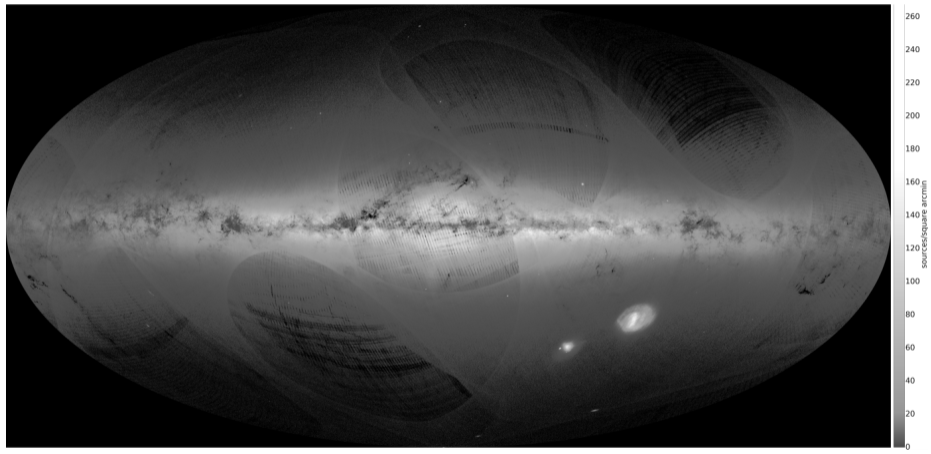
\includegraphics[width = 12cm, height = 6cm]{./Graficos/Capitulo_1/Gaia_DR1_Flux.png}} 
\caption{\scriptsize{ Sky distribution of all \textit{Gaia} DR1 sources in Galactic coordinates. The gray scale shows the source density which outlines well-known dust features along the Galactic plane in great detail. This scale also highlights non-astronomical artifacts. Image credits: CENTRA - University of Lisbon (part of the DPAC-CU9 visualization team). This figure is taken from (\cauthor{2016A&A...595A...2G} \citeyear{2016A&A...595A...2G}).}}
\label{fig:Gaia_DR1_Flux}
\end{figure}

In April $2018$ the \textit{Gaia} DR2 was released, consisting of astrometry, photometry, radial velocities, and information on astrophysical parameters and variability of sources brighter than magnitude $21.0$. In addition, epoch astrometry and photometry were provided for a modest sample of minor planets in the solar system (\cauthor{2018arXiv180409365G} \citeyear{2018arXiv180409365G}). This data release represents a major advance with respect to \textit{Gaia} DR1 in terms of completeness, performance, and richness of the data products corresponding to the first $22$ months of the mission. The data set contains celestial positions and the apparent magnitude brightness in G-band for approximately $1.7$ billion sources of which $1.3$ billion have additionally available parallaxes and proper motions \cauthor{2018arXiv180409366L} (\citeyear{2018arXiv180409366L}). There are four new key elements in this release: \textit{(i)} broad-band color information in the form of the apparent brightness in the $\textnormal{G}_\textnormal{BP}$ ($330-680\textnormal{nm}$) and $\textnormal{G}_\textnormal{RP}$ ($630-1050\textnormal{nm}$) bands, available for $1.4$ billion sources; \textit(ii) median radial velocities for some $7$ million source; \textit{(iii)} effective temperature, extinction, reddening, and radius and luminosity are provided for between $77$ and $161$ million sources; and \textit{(iv)} for a pre-selected list of $14\,000$ minor planets in the solar system epoch astrometry and photometry are provided (\cauthor{2018arXiv180409365G} \citeyear{2018arXiv180409365G}).\\ %The original sample of detections which were processed goes up to $52$ billion, but around $11$ billion were considered spurious and therefore did not take part in the cross-matching. Thus, the remaining $41$ billion transits were matched to $2\,583$ million sources, of which a significant number could be still spurious, have too few or poor observations leading to a final sample of $1693$ million sources \cauthor{2018arXiv180409366L} (\citeyear{2018arXiv180409366L}). For the bright sources ($\textnormal{G}\sim12\textnormal{mag}$), where parallax and proper motion data were already included in the \textit{Gaia} DR1, the new results represent a more accurate and fully independent of the \textit{Hipparcos} and \textit{Tycho} catalogs.\\

For \textit{Gaia} DR2 source are provided with broadband photometry in the $\textnormal{G}$,  $\textnormal{G}_\textnormal{BP}$, and  $\textnormal{G}_\textnormal{RP}$ bands (\cauthor{2017A&A...599A..32V} (\citeyear{2017A&A...599A..32V}); \cauthor{2017A&A...600A..51E} (\citeyear{2017A&A...600A..51E}); \cauthor{2018arXiv180409366L} (\citeyear{2018arXiv180409366L})). However, photometry is not perfect and strong systematic effects at the faint end of the survey $\textit{G}\sim19$, in crowded regions, and near bright stars are present. Specific treatment of crowded regions, and background estimation for the blue and red photometers lead to inconsistent measurements in different fluxes in the $\textnormal{G}$ and the $\textnormal{G}_\textnormal{BP}$, and  $\textnormal{G}_\textnormal{RP}$ bands in the sense that the sum of the flux values in the latter two bands may be significantly larger than that in $\textnormal{G}$ (whereas it is expected to be the quite same) (\cauthor{2018arXiv180409365G} \citeyear{2018arXiv180409365G}). \textit{Gaia} provides an `excess factor' entry to correct for possible photometric errors included if needed. 

%The major new element of solar information for \textit{Gaia} DR2 sources is provided by the broadband photometry in the $\textnormal{G}$,  $\textnormal{G}_\textnormal{BP}$, and  $\textnormal{G}_\textnormal{RP}$ bands (\cauthor{2017A&A...599A..32V} (\citeyear{2017A&A...599A..32V}); \cauthor{2017A&A...600A..51E} (\citeyear{2017A&A...600A..51E}); \cauthor{2018arXiv180409366L} (\citeyear{2018arXiv180409366L})). This suffers from strong systematic effects at the faint end of the survey $\textit{G}\sim19$, in crowded regions, and near bright stars. Insufficiently accurate background estimation is present in the photometric measurements from the blue and ed photometers, and from the lack of specific treatment of the prism spectra in crowded regions, where the overlapping of images of nearby sources is not yet accounted for. This basically leads to measured fluxes that are inconsistent between the $\textnormal{G}$ and the $\textnormal{G}_\textnormal{BP}$, and  $\textnormal{G}_\textnormal{RP}$ bands in the sense that the sum of the flux values in the latter two bands may be significantly larger than that in $\textnormal{G}$ (whereas it is expected that for normal spectral energy distributions the sum of fluxes in $\textnormal{G}_\textnormal{BP}$ and $\textnormal{G}_\textnormal{RP}$ should be comparable to that in $\textnormal{G}$) \cauthor{2018arXiv180409365G} (\citeyear{2018arXiv180409365G}). The \textit{Gaia} DR2 database counts with a quantitative indicator of this effect in the form of `excess factor' called \textit{phot\_bp\_rp\_excess\_factor} in the data archive in order to allow users to clean their samples and obtain reliable information.\\

In \autoref{fig:Gaia_DR2_Flux} and \autoref{fig:Gaia_DR2_FluxColor}, the sky distribution of all \textit{Gaia} DR2 sources in Galactic coordinates, and a map of the total flux measured in the $G_{RP}$, $G$, and $G_{BP}$ bands is shown. The sky map distribution shows in logarithmic scale the number of sources per square arcmin. The total flux map combines the integrated fluxes as observed in the $\textnormal{G}$,  $\textnormal{G}_\textnormal{BP}$, and  $\textnormal{G}_\textnormal{RP}$ bands, where the integrated flux map for each of the bands was used to color code the image according to a red, green, and blue channel. Here, it is evident the availability of homogeneous all-sky multi-band photometry in \textit{Gaia} DR2, offering a magnificent view of the Milky Way in color \cauthor{2018arXiv180409365G} (\citeyear{2018arXiv180409365G}). This represents the most detailed all-sky map in the optical to date. A remarkable improvement from \textit{Gaia} DR1 to \textit{Gaia} DR2 can be appreciated comparing \autoref{fig:Gaia_DR1_Flux} and \autoref{fig:Gaia_DR2_Flux} in which a much more complete and homogeneous sample is presented.\\  

\begin{figure}[!ht]
\centering
  \subfloat{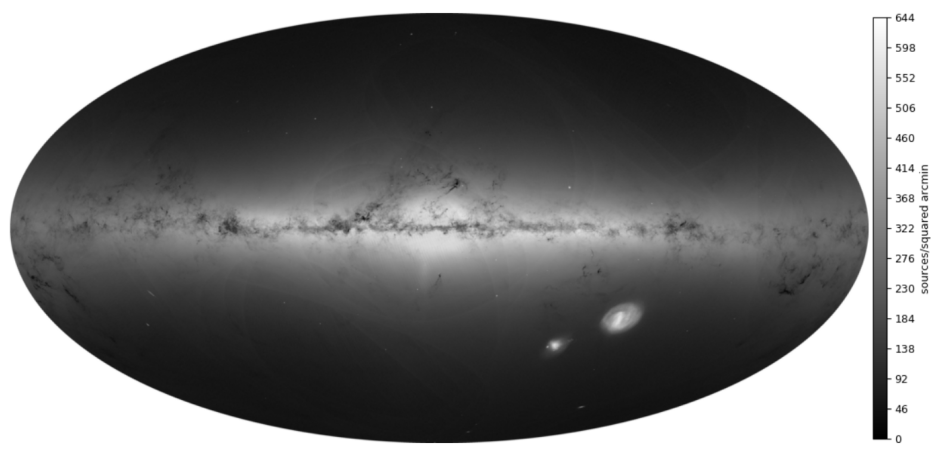
\includegraphics[width = 13cm, height = 6cm]{./Graficos/Capitulo_1/Gaia_DR2_Flux.png}} 
\caption{\scriptsize{ Sky distribution of all \textit{Gaia} DR2 sources in Galactic coordinates. This figure and the one in \autoref{fig:Gaia_DR2_FluxColor} are Hammer projections of the full sky.
The projection guarantees to have the same area per pixel (not strictly true because of pixel discretization). Each pixel is $\sim5.9$ square
arcmin. The color scale is logarithmic and represents the number of sources per square arcmin. The figure was taken from (\cauthor{2018arXiv180409365G} \citeyear{2018arXiv180409365G})}}
\label{fig:Gaia_DR2_Flux}
\end{figure}

\begin{figure}[!ht]
\centering
  \subfloat{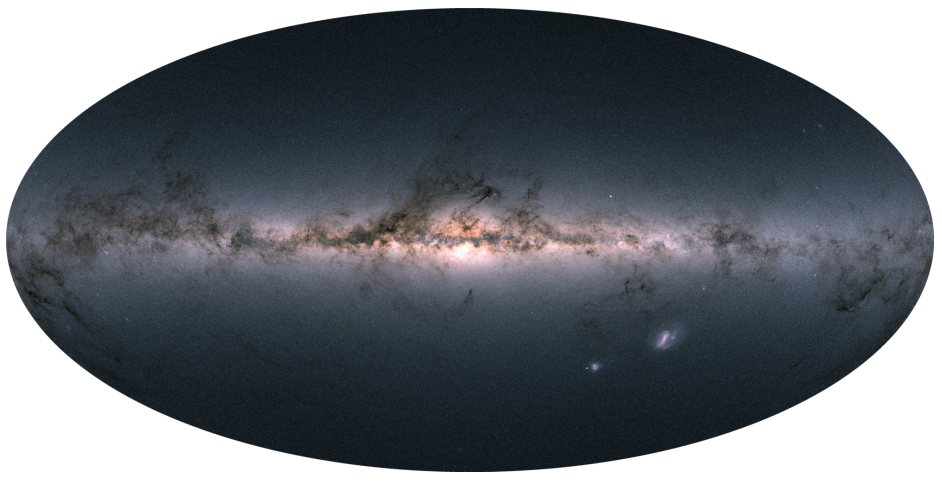
\includegraphics[width = 12.5cm, height = 6cm]{./Graficos/Capitulo_1/Gaia_DR2_FluxColor.png}} 
\caption{\scriptsize{  Map of the total flux measured in the $G_{RP}$, $G$, and $G_{BP}$ bands, where the flux in these bands is encoded in the red, green, and blue channel,
respectively. In some regions as in the lower left of the bulge there is a green region produced by lack of information in the $G_{BP}$ and $G_{RP}$ bands for a large number of sources. This kind of artifacts is also present in the region to the upper left of the Small Magellanic Cloud and at high Galactic
latitude to the right of the north Galactic pole region. The figure was taken from (\cauthor{2018arXiv180409365G} \citeyear{2018arXiv180409365G})}}
\label{fig:Gaia_DR2_FluxColor}
\end{figure}

In general, \textit{Gaia} is built to address questions on the formation and evolution of our Galaxy through the analysis of the distribution and kinematics of luminous and dark mass. By combining extinction deduced from stars, it is possible to construct the three-dimensional distribution of dust in our galaxy. In this way, \textit{Gaia} not only addresses the stellar contents, but also the interstellar matter in the Milky Way. \textit{Gaia} distances allow the derivation of absolute luminosities for stars which, combined with metallicities, allow the derivation of accurate individual ages, in particular for old subgiants, which are evolving from the main-sequence turn-off to the bottom of the red giant branch. One of the most striking and revolutionary results from this mission is the measurement of parallaxes, with hundreds of millions being accurate enough to derive high-quality color-magnitude diagrams and to make significant progress in stellar astrophysics. Star formation studies will benefit from the combination of \textit{Gaia} astrometry and photometry. On average, each star is measured astrometrically $\sim70$ times during five-year nominal operations phase. Sudden photometric changes in transient objects can be captured and the community can be alerted for follow-up observations. Periodic changes in photometry can be used to find (eclipsing) binaries and an improved census of double-lined systems based on spectroscopy will follow from the \textit{Gaia} data. A strong point of \textit{Gaia} in the exoplanet research field is the provision of an unbiased, volume-limited sample of Jupiter-mass planets in multi-year orbits around their host stars \cauthor{2014ApJ...797...14P} (\citeyear{2014ApJ...797...14P}). In addition, the astrometric data of \textit{Gaia} allow actual masses (rather than lower limits) to be measured. Besides this, the data will provide the detailed distributions of giant exoplanet properties (including the giant planet - brown dwarf transition regime) as a function of stellar-host properties with unprecedented resolution. %\textit{Gaia} will provide a census of orbital parameters and taxonomy in a single, homogeneous photometric system. A major scientific aim in the Local Group concerns the mutual, dynamical interaction of the Magellanic Clouds and the interaction between the Clouds and the Galaxy. Quasars form a special category of extragalactic sources for \textit{Gaia} as not only their intrinsic properties can be studied, but they can also be used in comparisons of optical and radio reference frames. Given the huge number of measurements, it is possible to exploit the redundancy in these corrections to conduct relativity tests or to use (residual of) the \textit{Gaia} data in more general fundamental-physics experiments.     


%==============================================================================================================================
\section{SuperWASP (Wide Angle Search for Planets)}\label{sec:SWASPdata}

Radial velocity surveys indicate that around $~1\%$ of solar neighborhood stars harbor hot Jupiter companions, and when invoking geometric arguments then $~10\%$ of these planets distributed in random orbits should transit their parent stars (\cauthor{2003ASPC..294..405S} (\citeyear{2003ASPC..294..405S}); \cauthor{2006PASP..118.1407P} (\citeyear{2006PASP..118.1407P})). Therefore, in random Galactic fields, roughly $1$ to $1000$ solar-type stars should exhibit transits lasting $\sim 2$hr with a period of a few days \cauthor{2006PASP..118.1407P} (\citeyear{2006PASP..118.1407P}). In particular, there is an apparent lack of transits due to the difficulty obtaining photometry of a sufficient number of solar-and late-type main-sequence stars. This was a strong reason back in the early 2000's to perform dense sampling to enable us to detect and closely examine the light curves of a range of transient phenomena \cauthor{2003ASPC..294..405S} (\citeyear{2003ASPC..294..405S}).\\

The \textit{SuperWASP} project is an exoplanet transit survey that has been automatically taking wide field images since $2004$. It is composed of basically two instruments (identical robotic telescopes), one located at the Observatorio del Roque de los Muchachos on La Palma, and the other one at the South African Astronomical Observatory in South Africa, continually monitoring the night sky, building up light curves of millions of unique objects (\cauthor{2006PASP..118.1407P} (\citeyear{2006PASP..118.1407P}); \cauthor{2008ApJ...675L.113W} (\citeyear{2008ApJ...675L.113W}); \cauthor{2010A&A...520L..10B} (\citeyear{2010A&A...520L..10B})). Each telescope consists of eight lenses (Canon $200$ mm f$/1.8$) feeding a $2048\times2048$ thinned CCD with a pixel size of $13.5 \mu \textnormal{m}$. This gives a field of view of $7.8\times7.8 \textnormal{deg}$ ($61\textnormal{deg}^2$) per camera \cauthor{2010A&A...520L..10B} (\citeyear{2010A&A...520L..10B}), a total field of view of $482\textnormal{deg}^2$, and an angular scale of $13.7\textnormal{px}^{-1}$ \cauthor{2006PASP..118.1407P} (\citeyear{2006PASP..118.1407P}). The delivered photometry accuracy is better than $1\%$ for objects having V$\sim7.0-11.5$. From $2006$ onwards a broadband filter was installed with a passband from $400$ to $700\textnormal{nm}$. The systems were designed to monitor fields with high cadence and they are capable of surveying the entire visible sky every $40$ minutes. The observation is carried out in $6$-$8$ fields at a similar declination and spaced apart approximately by one hour in right ascension each night. In order to avoid crowded fields close to the Galactic plane the observing strategy is altered. Thus a large part of mid-plane of the Milky Way galaxy is not sampled. Twice per night the exoplanet survey is interrupted to perform a full sky survey, a process that takes $40$ minutes as was said before \cauthor{2010A&A...520L..10B} (\citeyear{2010A&A...520L..10B}). Images are taken simultaneously from eight wide-angle cameras in each case throughout the night, offering as main product to the scientific community, light curves of individual stars \cauthor{2010A&A...520L..10B} (\citeyear{2010A&A...520L..10B})\\    

This surveys have the great advantage of requiring only relatively inexpensive, off-the-shelf equipment, which is then dedicated to the project. As said before, radial velocity surveys indicate that $\sim 1\%$ of stars between $7$ and $13$ mag may harbor hot Jupiters. Such a sample is necessary to answer questions about the formation and evolution of these planets, and how it is related to factors such as stellar metallicity, age, type, among others \cauthor{2003ASPC..294..405S} (\citeyear{2003ASPC..294..405S}). On the other hand, the main science aim of these systems is to search for bright transiting exoplanet systems suitable for spectroscopic follow-up observations \cauthor{2003ASPC..294..405S} (\citeyear{2003ASPC..294..405S}). \textit{SuperWASP} DR1 contains light curves data and images from $2$nd May $2004$ up to $9$th August $2008$ for the North hemisphere, and from $13$th February $2006$ and go through to the $27$th May $2008$ \cauthor{2010A&A...520L..10B} (\citeyear{2010A&A...520L..10B}). The data set contains in total $3\,631\,972$ raw images and $17\,970\,937$ light curves. In \autoref{fig:SWASP_DR1_Flux}, the projection of the average number of data points per light curve in the \textit{SuperWASP} DR1 is shown. Moreover, the format of the data lends itself to non-exoplanet research also, for example variable star studies \cauthor{2007A&A...467..785N} (\citeyear{2007A&A...467..785N}) and single star studies \cauthor{2007MNRAS.380.1230C} (\citeyear{2007MNRAS.380.1230C})\\  

\begin{figure}[!ht]
\centering
  \subfloat{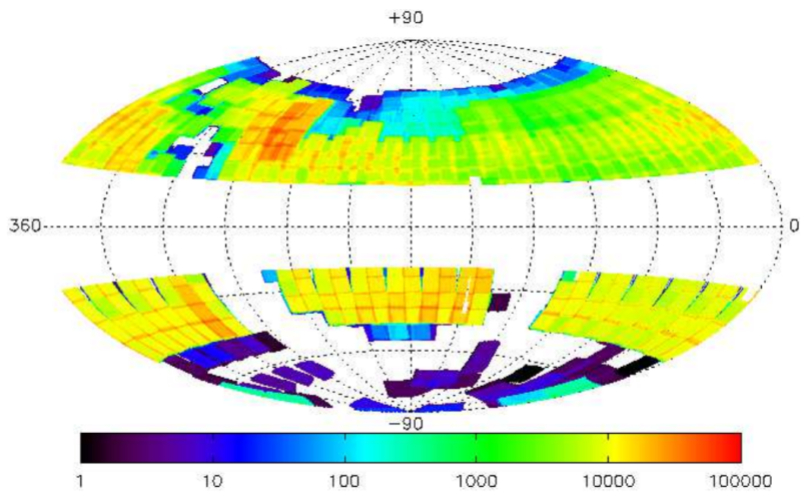
\includegraphics[width = 12cm, height = 7cm]{./Graficos/Capitulo_1/SWASP_DR1.png}} 
\caption{\scriptsize{  Hammer-Aitoff projection of the average number of data
points per light curve available in this \textit{SuperWASP} DR1. \cauthor{2010A&A...520L..10B} (\citeyear{2010A&A...520L..10B})}}
\label{fig:SWASP_DR1_Flux}
\end{figure}

\begin{table}[]
\centering
\caption{Data available for each photometric point \cauthor{2006PASP..118.1407P} (\citeyear{2006PASP..118.1407P}) in the \textit{SuperWASP} DR1 \cauthor{2010A&A...520L..10B} (\citeyear{2010A&A...520L..10B})}
\label{tab:SWASP_params}
\scalebox{0.9}{
\begin{tabular}{lll}
\hline Name          & Unit                              & Description                    \\ \hline \hline
              & Stored in the light curve on disk &                                \\ \hline
TMID          & s                                 & Mid-time of exposure           \\
FLUX2         & micro Vega                        & Processed flux                 \\
FLUX2\_ERR    & micro Vega                        & Processed flux error           \\
TAMFLUX2      & micro Vega                        & TAMUZ corrected processed flux \\
TAMFLUX2\_ERR & micro Vega                        & TAMUZ flux error               \\
CCDX          & 1/16th of pixel                   & X position on the CCD          \\
CCDY          & 1/16th of pixel                   & Y position on the CCD          \\
IMAGEID       & \_                                & Unique image ID                \\
FLAG          & \_                                & Bitmask                        \\ \hline
\end{tabular}
}
\end{table}

Each light curve is stored in binary FITS table format. In \autoref{tab:SWASP_params}, the columns in the FITS file are listed. Each row corresponds to a data point in the light curve and is the result of aperture photometry of the images by a pipeline, as described in \cauthor{2005MNRAS.364.1091K} (\citeyear{2005MNRAS.364.1091K}). This results in a processed flux measurement (\textit{FLUX2}) of each object from each image. However, further to this flux, a \textit{TAMUZ} corrected flux is given, which gives a more consistent measurement between different cameras and years (\cauthor{2007MNRAS.380.1230C} (\citeyear{2007MNRAS.380.1230C}); \cauthor{2010A&A...520L..10B} (\citeyear{2010A&A...520L..10B})). The \textit{TAMUZ} flag is a bit-mask; if corrections has been made then this will be $32$, if it is zero then the \textit{TAMUZ} flux and error will be a copy of \textit{FLUX2} values. \textit{TMID} is the heliocentrically corrected mid-point of the exposure in seconds after $2004-01-01\textnormal{T}00:00:00$ and can be converted to \textit{HJD} using \autoref{eq:HJD_Swasp}.\\ 

\begingroup
\Large
\begin{equation}
 \textnormal{HJD} = \frac{\textnormal{TMID}}{86\,400} + 2453005.5 
 \label{eq:HJD_Swasp}
\end{equation}
\endgroup

\begingroup
\Large
\begin{equation}
 \textnormal{mag} = 15.0 - 2.5 \log(\textnormal{flux})
 \label{eq:Mag_Swasp}
\end{equation}
\endgroup \\

In both flux cases the units are given as micro Vegas, this gives a simple conversion given by \autoref{eq:Mag_Swasp}, where flux is in micro Vegas. This implies a flux of $1.0$ micro Vega corresponds to $15$th mag, and $10^6$ micro Vega; $0th$ mag \cauthor{2010A&A...520L..10B} (\citeyear{2010A&A...520L..10B}). Last but not least, the names of each star in the \textit{SuperWASP} are listed as follows, $1\textnormal{SWASP}~~\textnormal{Jhhmmss.ssSddmmss.s}$. Therefore, following this convention, a unique identifier is used. 

%==============================================================================================================================
\section{Sco OB2 (ScoCen)}\label{sec:ScoOB2}

This project was centered in a region of the night sky known as Sco OB2 or ScoCen. The region was classified as an OB association by \cauthor{Blaauw46} (\citeyear{Blaauw46}) due to the fact that back in the days only more massive stars were achievable through photometric studies mainly made up of O/B-type stars. However, nowadays is quite clear that OB associations contain members across the mass spectrum, including not only O-and B-type stars, but also intermediate mass A/F stars, lower-mass G/K/M stars, and very low-mass free floating substellar objects. Stars below $< 1.5 \textnormal{M}_\odot$ comprise the dominant component of OB associations which is equivalent to say that the vast majority correspond to low-mass stars \cauthor{2016MNRAS.461..794P} (\citeyear{2016MNRAS.461..794P}).\\

ScoCen is the nearest OB association to the Sun that has recently formed stars \cauthor{2018MNRAS.tmp..210W} (\citeyear{2018MNRAS.tmp..210W}), turning it into one of the most important OB associations to study the star-formation process, the origin of the initial mass function (IMF), to investigate how high-and low-mass stars are distributed in space during the evolution of the giant molecular clouds and the star-forming process \cauthor{1989A&A...216...44D} (\citeyear{1989A&A...216...44D}) and the interaction of early-type stars with the interstellar medium. In particular, these regions offer an indispensable good sample to characterize and study the formation of planets and their evolution allowing us to estimate the timescale in which gaseous disks dissipate \cauthor{2018arXiv180200878M} (\citeyear{2018arXiv180200878M}), and the potential of a star to host habitable exoplanets which is directly related to the environment on which stars are born and spend the first few million years of their lives \cauthor{2018MNRAS.tmp..210W} (\citeyear{2018MNRAS.tmp..210W}). Also indispensable for direct imaging of brown dwarf and planetary mass companions; star disk interaction of young stars, imaging of debris disks, and evolution of gas-rich and dusty debris disks \cauthor{2016MNRAS.461..794P} (\citeyear{2016MNRAS.461..794P}). It is widely known that stars tend to form in clusters, however, stars with ages around $\sim10 \textnormal{Myr}$ observed in bound clusters only account for a $10\%$ in total. A likely explanation to this is based on how stars are formed embedded within molecular clouds, which are indeed held together by their own gravitational potential of both stars and gas \cauthor{2018MNRAS.tmp..210W} (\citeyear{2018MNRAS.tmp..210W}), but when the intern feedback disperses the gas, then the cluster starts to disperse and expand. This is why we can observe low-density groups of young stars known as associations that can keep on evolving and disperse in the galactic field.\\

Since its discovery, the region has been divided in three main subgroups known as \textit{Upper Scorpius} (US), \textit{Upper Centaurus-Lupus} (US), and \textit{Lower Centaurus-Crux} (LCC) \cauthor{Blaauw46} (\citeyear{Blaauw46}), with mean parallaxes of $6.9$, $7.1$, and $8.5$mas or distances of $145$, $143$, and $118$pc respectively \cauthor{2015yCat..74163108R} (\citeyear{2015yCat..74163108R}). In recent studies as those of \cauthor{2018MNRAS.tmp..210W} (\citeyear{2018MNRAS.tmp..210W}) this OB association has been proposed to lie in a distance range between $\sim100$ to $150$ pc covering almost $90$-deg on the sky or $2000\textnormal{deg}^2$. The estimated ages of US, UCL, and LCC are $11$, $16$, and $17$ Myr respectively, though it is clear that there exists a considerable spread (\cauthor{1989A&A...216...44D} \citeyear{1989A&A...216...44D}; \cauthor{2018MNRAS.tmp..210W} \citeyear{2018MNRAS.tmp..210W}). US contains a vast number of stars that has been thoroughly studied in the past decades, however, it is clear the LCC and UCL are more spread out decreasing the concentration and making the task more tricky due to the closer overlap with the Galactic plane \cauthor{2015yCat..74163108R} (\citeyear{2015yCat..74163108R}) making the separation of actual member really difficult. High quality data is needed, as measurements of star motions which allows the study of the separation of UCL and LCC members as provided by surveys as \textit{Hipparcos} \cauthor{1999AJ....117..354D} (\citeyear{1999AJ....117..354D}) and \textit{Gaia} DR1-DR2 (\cauthor{2012yCat..74163108R} \citeyear{2012yCat..74163108R}; \cauthor{2016MNRAS.461..794P} \citeyear{2016MNRAS.461..794P}; \cauthor{2018MNRAS.tmp..210W} \citeyear{2018MNRAS.tmp..210W}). \textit{Gaia} DR2 provides provides a remarkable improvement in parallaxes and proper motions of stars for the ScoCen region that for example benefits studies of the dynamical situation of the cluster to prove expansion, and constraint the initial conditions as those performed by \cauthor{2018MNRAS.tmp..210W} (\citeyear{2018MNRAS.tmp..210W}). In \autoref{fig:ScoCen_Mamajek}, a current sample of $433$ ScoCen members was used by \cauthor{2018MNRAS.tmp..210W} (\citeyear{2018MNRAS.tmp..210W}) to add additional information to the known properties of the OB association cross-matching \textit{Gaia} DR1 parallaxes and proper motion for a few of these sources.\\   

\begin{figure}[!ht]
\centering
  \subfloat{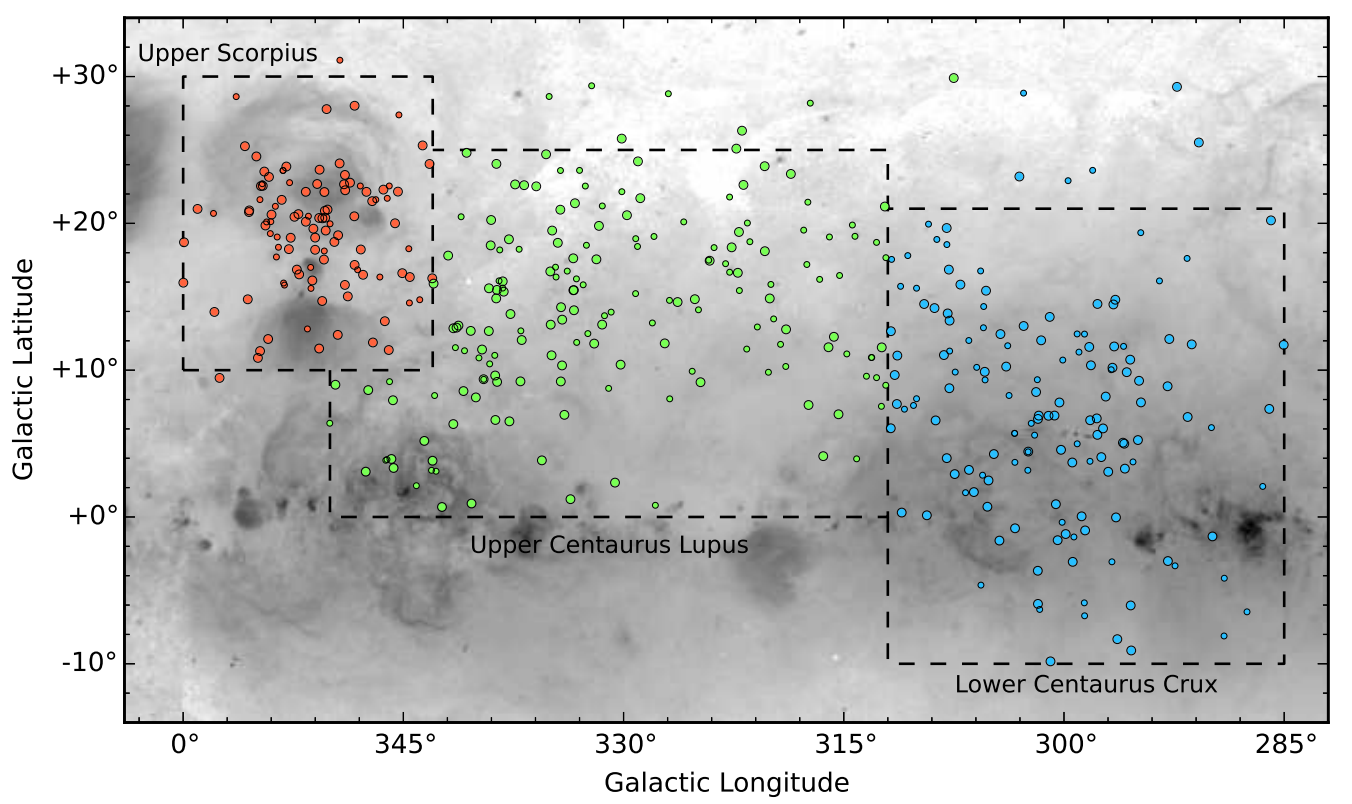
\includegraphics[width = 15cm, height = 8.5cm]{./Graficos/Capitulo_1/ScoCen.png}} 
\caption{\scriptsize{ Sco OB2 association in galactic coordinates. The dashed-line squares represent from top to bottom the Upper Scorpius, Upper Centaurus-Lupus, and Lower Centaurus-Crux regions as defined by \cauthor{Blaauw46} (\citeyear{Blaauw46}) and redefined by \cauthor{1999AJ....117..354D} (\citeyear{1999AJ....117..354D}). The sample corresponds to a total number of $433$ stars colored according to which of the three subgroups they nominally belong to. This figure is taken from \cauthor{2018MNRAS.tmp..210W} (\citeyear{2018MNRAS.tmp..210W}).}}
\label{fig:ScoCen_Mamajek}
\end{figure}

In \autoref{fig:ScoCen_Mamajek} a modified version of the original boundaries \cauthor{Blaauw46} (\citeyear{Blaauw46}) for the subgroups as re-defined by \cauthor{1999AJ....117..354D} (\citeyear{1999AJ....117..354D}) is presented. In general, the US, UCL, and LCC subgroups have been limited in total proper motion to $\mu < 47$, $12 < \mu < 55$, and $15 < \mu < 55$ mas respectively, and $\mu^*_\alpha < 10$ and $\mu_\delta < 30$ mas for the three subgroups \cauthor{2016MNRAS.461..794P} (\citeyear{2016MNRAS.461..794P}). Additionally, the low-mass population in ScoCen has been studied before focusing on binary properties, circumstellar disks, stellar ages, eclipsing binaries, and low-mass stars and brown dwarfs. This is particularly useful to study the early evolution of low-mass stars and substellar objects which requires an excellent characterization of young low-mass objects \cauthor{2018arXiv180200878M} (\citeyear{2018arXiv180200878M}) to give a glimpse into the state of a group of stars directly after their formation, and using a unique age-calibrated sample \cauthor{2015yCat..74163108R} (\citeyear{2015yCat..74163108R}).  

%==============================================================================================================================
\section{Exoplanetary Rings: the particular case of J1407}\label{sec:Exorings}

% Mamamjek 2012  \cauthor{2012AJ....143...72M} (\citeyear{2012AJ....143...72M}
% Kenworthy 2015 \cauthor{2015MNRAS.446..411K} (\citeyear{2015MNRAS.446..411K}
% \cauthor{} (\citeyear{}

Exoplanetary transits have been a major topic in astrophysics since the 1990's when the first exoplanets were discovered. The vast sample was mainly conformed by giant planets and Hot-Jupiters. Since then, different techniques as radial velocity, transit photometry, direct imaging, among others have been explored and refined to achieve lower limits which allows us to detect earth-like planets. However, less is said about circumplanetary disks (proto-satellite disks) that likely existed during the first $\sim10^7$ years \cauthor{2012AJ....143...72M} (\citeyear{2012AJ....143...72M}), although, there are studies investigating the detectability of thin, discrete planetary rings similar to Saturn's as reported in (\cauthor{2004ApJ...616.1193B} \citeyear{2004ApJ...616.1193B}; \cauthor{2009ApJ...690....1O} \citeyear{2009ApJ...690....1O}). Circumplanetary disks are extended, then, the probability that a randomly oriented system exhibits eclipses may not be negligible. In \cauthor{2012AJ....143...72M} (\citeyear{2012AJ....143...72M}), it was estimated that a survey of $\sim10^4$ young ($~10$ million year old) post-accretion pre-main-sequence stars monitored for $~10$ years should yield at least a few deep eclipses from circumplanetary disks and disks surrounding low-mass companion stars.\\
 
In $2012$, \cauthor{2012AJ....143...72M} (\citeyear{2012AJ....143...72M}) identified a star with a remarkable light curve among the \textit{SuperWASP} DR1 data (\cauthor{2006PASP..118.1407P} \citeyear{2006PASP..118.1407P}; \cauthor{2010A&A...520L..10B} \citeyear{2010A&A...520L..10B}) for the new ScoCen members known as \textit{1SWASP J1407.93-394542.6 = ASAS J140748-3945.7} (hereafter `J1407'). This star is known to be part of the \textit{Upper Centaurus-Lupus} subgroup of ScoCen \cauthor{1999AJ....117..354D} (\citeyear{1999AJ....117..354D}) lying at a distance of $128\pm13$ pc derived from a kinematic analysis, similar to the UCL members as reported by \cauthor{2012AJ....143...72M} (\citeyear{2012AJ....143...72M}). Using this distance, and three sets of evolutionary tracks, the star is known to be located in the HR-diagram at $\log$ T $= 3.66$ and $\log$ L$/$L $=$ -0.47 with a stellar mass of $\sim0.9$M$_\odot$. The young star ($\sim 16$ Myr) appears to be a weak-lined T Tauri star, not hosting its own circumstellar disk \cauthor{2015MNRAS.446..411K} (\citeyear{2015MNRAS.446..411K}). \\ 

In particular, the light curve exhibited a notorious long, deep, and complex eclipse event centered on $2007$ April $29$th as seen in the \textit{SuperWASP} V-magnitude photometry, and with portions of the dimming confirmed by the All Sky Automated Survey (\textit{ASAS}) \cauthor{2002AcA....52..397P} (\citeyear{2002AcA....52..397P}) data as it is shown in \autoref{fig:Mamajek_J1407_1}. This unusual eclipse is similar to those seen in $\epsilon$ Aurigae (\cauthor{2002ASPC..279..121G} \citeyear{2002ASPC..279..121G}; \cauthor{2010Natur.464..870K} \citeyear{2010Natur.464..870K}; \cauthor{2011A&A...530A.146C} \citeyear{2011A&A...530A.146C}), KH 15D \cauthor{2006ApJ...644..510W} (\citeyear{2006ApJ...644..510W}), EE Cep (\cauthor{Mikolajewski1999} \citeyear{Mikolajewski1999}; \cauthor{2003A&A...403.1089G} \citeyear{2003A&A...403.1089G}; \cauthor{2010ASPC..435..423G} \citeyear{2010ASPC..435..423G}) which are periodically occulted by extended objects. The \textit{SuperWASP} DR1 photometry contains approximately $29\,000$ epochs during $206$ dates between HJD $2453860$ ($2006.34$) and HJD $2455399$ ($2010.56$), with median photometric precision  of $0.023$ mag. On the other hand, the \textit{ASAS} archive contains an extremely long time baseline light curve for J1407, with photometry provided over 599 dates between HJD $2451887$ $2001$ February and HJD $2455088$ $2009$ September. In this dataset sample, a minor but sustained dip in magnitudes between $2001.20$ and $2001.24$, approximately $14$ days and with depth $\sim 0.2$ mag is also observed.\\

Five multi-day dimming events of $>0.5$ mag were identified, with a $3.3$ mag deep eclipse between HJD $2454213$ ($2007$ April $23$rd) and HJD $ 2454227$ ($2007$ May $7$th), bracketed by two pairs of $\sim 1$ mag eclipses symmetrically occurring $\pm 12$ days and $\pm 26$ days before and after, as reported in \cauthor{2012AJ....143...72M} (\citeyear{2012AJ....143...72M}). The light curve for the \textit{SuperWASP} data is dominated by a quasi-sinusoidal component with amplitude $\sim0.1$ mag and periodicity of $3.211$ days consistent with rotational modulation of starspots, typical for young active stars \cauthor{2008ApJ...687.1264M} (\citeyear{2008ApJ...687.1264M}). A firm lower limit on the period of $850$ days was placed by \cauthor{2012AJ....143...72M} (\citeyear{2012AJ....143...72M}). In right panel of \autoref{fig:Mamajek_J1407_1}, both data from nightly averaged \textit{SWASP}, and \textit{ASAS} is shown, where two pairs of multiday dips named $A1$ and $A2$ separated by $\sim24$ days, and $B1$ and $B2$ separated by $\sim51.5$ days can be observed. From this figure, it is inferred that probably a disk with large gaps may be producing extra dips in between those pairs mentioned above, because they appear to be free of extinction lasting just for a couple of days.\\      
 
\begin{figure}[!ht]
\centering
  \subfloat{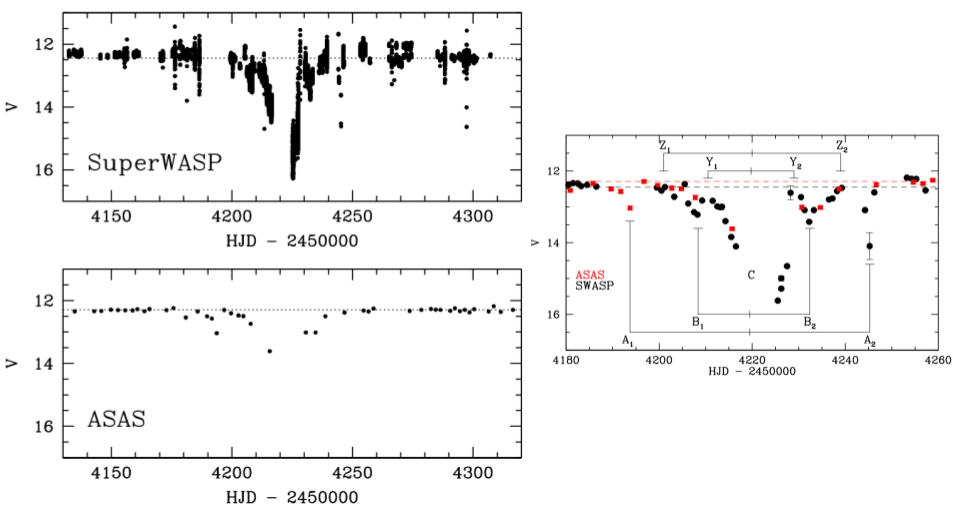
\includegraphics[width = 16cm, height = 10cm]{./Graficos/Capitulo_1/Mamajek_J1407.png}} 
\caption{\scriptsize{ \textbf{Top left:} \textit{SuperWASP} V-magnitude light curve for J1407. \textbf{Bottom left:} \textit{ASAS} V-magnitude data for J1407 . The data was obtained during early $2007$. The abscissa corresponds to the Heliocentric Julian Date minus $2450000$. Thus, $2007$ January $1$st midnight corresponds to HJD $2454101.5$. The eclipse was seen in both photometric data sets. \textbf{right:} \textit{SuperWASP} and \textit{ASAS} photometry for the $2007$ April-May eclipse event(s). \textit{ASAS} photometry is a single measurement each night, whereas the \textit{SuperWASP} magnitudes are nightly median values. The figures are taken from \cauthor{2012AJ....143...72M}(\citeyear{2012AJ....143...72M})}}
\label{fig:Mamajek_J1407_1}
\end{figure}

Having said that, it is quite likely that the observed features  in the light curve of J1407 are being produced by a low-mass object hosting a disk with significant substructure composed of thin dust debris belts, or rings as it is shown in \autoref{fig:Mamajek_J1407} where a non-unique disk model was fit to the \textit{SuperWASP} observations. Nevertheless, a low mass secondary star with a disk, a brown dwarf, and a gas giant planet could perhaps be some plausible explanations of the features observed. This young, Li-rich K5 star, shows a lack of infrared excess emission at long (\textit{WISE}, \cauthor{2010AJ....140.1868W} (\citeyear{2010AJ....140.1868W}) and short wavelengths (\textit{WISE}, \cauthor{2006AJ....131.1163S} (\citeyear{2006AJ....131.1163S})  and no accretion indicators \cauthor{2012AJ....143...72M}(\citeyear{2012AJ....143...72M}) which clearly suggests that the mass of the unseen object is much lower than that of the solar-mass K star. On the other hand, as was stated before, the disk must be large, so the probability of a system hosting one which is oriented in such a way that can occult the star and produce the transit is tiny, but not zero. The lifetime of a second phase Jupiter's circumstellar disk is estimated to be of order a million years (\cauthor{2009euro.book...59C} (\citeyear{2009euro.book...59C}); \cauthor{2005A&A...434..343A} (\citeyear{2005A&A...434..343A}); \cauthor{2010AJ....140.1168W} (\citeyear{2010AJ....140.1168W}), thus, the lifetime of a circumplanetary disk at $25$ AU could be about $10$ times longer (or of order $\sim10^7$ years) or at $100$ AU $100$ times longer (or of order $\sim10^8$ years) \cauthor{2012AJ....143...72M} (\citeyear{2012AJ....143...72M}). Having said that, it is clear that the lifetime of a circumplanetary disk could be longer for planets at large semi-major axis, then light detected from outer exoplanets may also come from such a disk. According to \cauthor{2015MNRAS.446..411K} (\citeyear{2015MNRAS.446..411K}), the complex ring system appears to occupy more than $0.15$ of its Hill radius, much larger than its Roche radius, suggesting a ring structure in transition.\\

\begin{figure}[!ht]
\centering
  \subfloat{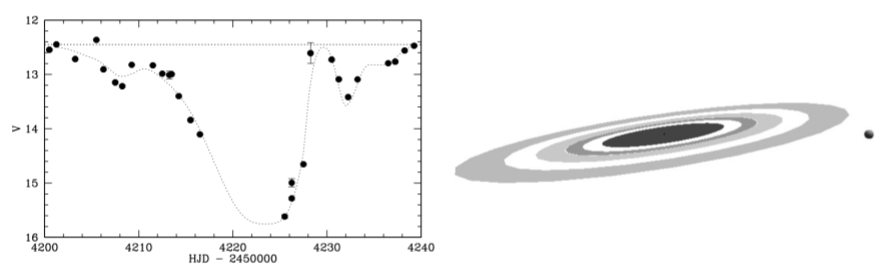
\includegraphics[width = 15cm, height = 5cm]{./Graficos/Capitulo_1/Rings.png}} 
\caption{\scriptsize{ \textbf{left:} Simple, non-unique model in an attempt to fit the nightly averaged data obtained by the \textit{SuperWASP} observations. The model contains an object orbiting J1407 composed by a thick inner disk, a gap, and two rings with a smaller gap between them. \textbf{right:} Diagram of J1407's dust disk model, whose corresponding light curve is shown in the left panel. The dark dot corresponds to J1407 to scale (R = $0.96$R$_\odot$). The figures are taken from \cauthor{2012AJ....143...72M}(\citeyear{2012AJ....143...72M})}}
\label{fig:Mamajek_J1407}
\end{figure}

Summing up, this kind of eclipses seen among young stars may provide useful constraints on either circumsecondary or circumplanetary disk structure and the early evolution of planets and/or satellites because they constitute remarkable laboratories for testing these scenarios. Same can be said in the case of J1407, regardless of the nature of the disked companion. Predicting when the next eclipse will happen is vital to planning an extensive and detailed observing campaign, and also because this object offers the opportunity to analyze a young substellar object and possibly resolve the disk with ring-like structure spectrally and spatially \cauthor{2015MNRAS.446..411K} (\citeyear{2015MNRAS.446..411K}). Additional constraints based on high spectral resolution and precision RV measurements, combined with orbital periods ruled out by photometric monitoring and dynamical arguments show that the companion of J1407 is a substellar object and likely to be a planetary mass or brown dwarf mass object. The ring system is also considerably larger than the Roche radius for the secondary companion, suggesting that the system may be in a transitional state where exomoons are in process of formation. All models imply a ring system for J1407 that fills at least $0.15$ of the Hill sphere and is significantly larger than the Roche radius \cauthor{2015MNRAS.446..411K} (\citeyear{2015MNRAS.446..411K}). These large rings are unstable on long-timescales and will ultimately accrete to form exomoons, contrasting with solar system models where moons are formed from gradual overflow over the Roche radius \cauthor{2012Sci...338.1196C} (\citeyear{2012Sci...338.1196C}).   
%*****************************************
\chapter{\textbf{Model and Samples}} \label{ch: Model}
%*****************************************
\vspace{0.5cm} 

%============================================================================================================================================================
\section{Introduction}

In this chapter, we present an analysis of the occurrence of exoplanetary ringed systems. The first step consists in proposing a probability for the transits based on five different probabilities: the probability of a star harboring a planet in orbit, the probability of this planet having material around which could coalesce and form rings, the probability of observing the transit giving general geometric constraints, the probability of observing at least one transit during the nominal five-year \textit{Gaia} mission, and the probability of rings around a planet to be present at the moment of the observations. In order to solve this, we proposed a Monte-Carlo approach in which the most important parameters involved in this probability are simulated as could be the stellar mass and the planetary mass-period distributions. These distributions follow regular power laws making the Monte-Carlo suitable for our purpose. On the other hand, as we also count with an analytic function the same process was addressed and compared to the Monte-Carlo results.\\

The section is organized as follows: in \autoref{sec:PowerLawSec} the basis of the power law and Monte-Carlo approach is presented. The application of this method to planetary mass-period distribution and stellar IMF is addressed in \autoref{ref:PM_ExoPlanet} and \autoref{sec:StellarMAS_IMF} . Finally, in \autoref{sec:DetectionProbability} the proposed solution and comparison between the Monte-Carlo and the analytic approaches is presented. 

%============================================================================================================================================================

%============================================================================================================================================================
\section{Power Law Distributions} \label{sec:PowerLawSec}

It is well-known that the stellar mass, and exoplanetary mass and orbital period distributions can be described by power laws. As those parameters are essential in our formulation for the probability of exoplanetary rings transits, and the subsequent analysis, we must pay attention to how model samples which can reproduce faithfully the observation.\\

%A power law distribution can be defined as the relative change of two quantities, which are related through a common exponent. In other words, we can predict the change in one of the variables once the exponent and an initial set of values for the second variable are known. 
A power law distribution is defined as a functional relationship of a variable $N$ as a function of a variable $X$. The relative change in one of the variables induces a change in the other, modulated by one of the variables to a given power.   
Mathematically speaking, we define a power law distribution as \autoref{eq:PowerLaw}, where $N$ and $X$ are the variables, and $\alpha$ is the exponent relating the relative change between them and it is assumed $\alpha \neq 1$. Generally, the variable $N$ refers to the number of objects one would expect to find in a given interval $x_1 \leq X \leq x_2$, where the variable $X$ in our particular case may refer to the planetary period, planetary mass, stellar mass or any other parameter which we want to study.\\ 

\begingroup
\Large
\begin{equation}
 \frac{\textnormal{dN}}{\textnormal{dX}}~~\propto~~\textnormal{X}^{-\alpha}
 \label{eq:PowerLaw}
\end{equation}
\endgroup\\

%Power-laws can consist of a single or multiple exponents relating two or more variables. 
Power-laws can have single or multiple components described by different exponents. The easiest case is the single power law which has the mathematical form shown in \autoref{eq:PowerLaw}. However, the equation lacks a proportionality constant or normalization constant which must be found with boundary conditions. Therefore, \autoref{eq:PowerLaw} can be rewritten in a more general fashion as \autoref{eq:PowerLaw_1}, where $A$ corresponds to the normalization constant and can be found using \autoref{eq:NormConst} with $\gamma = 1 - \alpha$.\\

\begingroup
\Large
\begin{equation}
 \frac{\textnormal{dN}}{\textnormal{dX}}~~=~~\frac{\textnormal{X}^{-\alpha}}{A}~~~~~~~;~~~~~~~x_1 ~~\leq ~~\textnormal{X}~~ \leq ~~\textnormal{x}_2
 \label{eq:PowerLaw_1}
\end{equation}
\endgroup\\

\begingroup
\Large
\begin{equation}
 \textnormal{A}~~=~~\int_{\textnormal{x}_1}^{\textnormal{x}_2} X^{-\alpha} \textnormal{dX}~~=~~\frac{\textnormal{x}_2^{1 - \alpha} - \textnormal{x}_1^{1 - \alpha}}{1 - \alpha}~~=~~\frac{\textnormal{x}_2^{\gamma} - \textnormal{x}_1^{\gamma}}{\gamma} 
 \label{eq:NormConst}
\end{equation}
\endgroup\\

Furthermore, we can define the cumulative distribution function (CDF) $F(X)$, which will give us all the accumulated probability less than or equal to $X$. It is widely used to determine the probability of an observation being greater than a certain value, or between two values. The CDF will be of great importance in \autoref{sec:MCSec} where the randomly distributed variable is obtained by making use of it to generate the real variable. The mathematical form of the CDF is given in \autoref{eq:CDF} where the upper limit in the integral $x$ here refers to a value between the upper limit ($x_1$) and lower limit ($x_2$) over which one wants to generate the distribution.\\ 

\begingroup
\Large
\begin{equation}
 \textnormal{F}(\textnormal{x})~~=~~\textnormal{A}^{-1} \int_{\textnormal{x}_1}^{\textnormal{x}} \textnormal{t}^{-\alpha} \textnormal{dt}~~=~~\frac{\textnormal{x}^{\gamma} - \textnormal{x}_1^{\gamma}}{\textnormal{x}_2^{\gamma} - \textnormal{x}_1^{\gamma}}
 \label{eq:CDF}
\end{equation}
\endgroup\\

Subsequently, if the random variable is distributed uniformly between $0$ and $1$, one can generate the real variable by inverting the CDF shown in \autoref{eq:CDF} which leads to \autoref{eq:RandomVar}. As expected, if one evaluates the last equation in $y = 0$ and $y = 1$ which are the extreme values of the random variable, the result is $x = x_1$ and $x = x_2$ respectively in the real variable.\\

\begingroup
\Large
\begin{equation}
  \begin{align*}
    \textnormal{y} & ~~=~~  \textnormal{F}(\textnormal{x}) ~~=~~ \frac{\textnormal{x}^{\gamma} - \textnormal{x}_1^{\gamma}}{\textnormal{x}_2^{\gamma} - \textnormal{x}_1^{\gamma}} \\[10pt]
    \textnormal{x} & ~~=~~  (y~ (~\textnormal{x}_2^{\gamma} - \textnormal{x}_1^{\gamma}~) + \textnormal{x}_1^{\gamma})^{1/\gamma}
    \label{eq:RandomVar}
  \end{align*}
\end{equation}
\endgroup\\

The planetary mass-period distribution, and the stellar mass distribution will be generated following the simple power law explained above with a Monte-Carlo process in \autoref{sec:MCSec}. Although a different method was also explored for the planetary mass-period distribution due to a possible weakly dependence in both parameters (\cauthor{1538-3881-134-5-2061} \citeyear{1538-3881-134-5-2061}; \cauthor{2002ApJ...568L.113Z} \citeyear{2002ApJ...568L.113Z}), we decided to keep the power law method to model them as it is also widely used and studied in literature (\cauthor{2010EAS....41..107N} \citeyear{2010EAS....41..107N}; \cauthor{2008PASP..120..531C} \citeyear{2008PASP..120..531C}; \cauthor{2006ApJ...646..505B} \citeyear{2006ApJ...646..505B}).  

\section{Exoplanets: Period-Mass Distributions} \label{ref:PM_ExoPlanet}

In order to draw a reliable distribution sample of period and mass for exoplanets, we used two different approaches. The first approach uses the $\beta$-distribution because there exists a correlation between the period and mass of an exoplanet as shown by \cauthor{2002ApJ...568L.113Z} (\citeyear{2002ApJ...568L.113Z}). This makes the distribution analysis not suitable to be addressed by two independent power laws in order to describe the joint period-mass distribution. Alternatively, one can assume that as the correlation is weak, then each variable can be treated as independent and the distributions may be generated using single power laws as it is also widely explored by other authors \cauthor{2010EAS....41..107N} (\citeyear{2010EAS....41..107N}). Therefore, as there exist two different forms to address the generation of these distributions, both ways were explored and implemented in this work.\\

In \autoref{subsec:BetaDist} and \autoref{subsec:SPLDist}, the method is widely explained taking into account the different observations and arguments as shown in \cauthor{2002ApJ...568L.113Z} (\citeyear{2002ApJ...568L.113Z}) and \cauthor{2010EAS....41..107N} (\citeyear{2010EAS....41..107N}). 

\subsection{\texorpdfstring{$\beta$-}Distribution} \label{subsec:BetaDist}

Using a dataset of 66 exoplanets \cauthor{2002ApJ...568L.113Z} (\citeyear{2002ApJ...568L.113Z}) explored a possible correlation between the mass and period. Subsequently \cauthor{1538-3881-134-5-2061} (\citeyear{1538-3881-134-5-2061}) using a data set of 233 exoplanets supported this idea measuring a positive correlation coefficient of $0.1762$. As a result of the positive correlation, describing the distribution as two independent power laws it is not correct, and a new coupled positively correlated function is needed to describe the problem. However, generating this type of distributions needs $\beta$-distributed random variables which was not provided until \cauthor{2004CMS...46.397M} (\citeyear{2004CMS...46.397M}) work.\\

The probability distribution function (pdf) on a finite interval (c,d), $-\infty < \textnormal{c} < \textnormal{d} < \infty $, indexed by two positive parameters $\alpha$ and $\beta$ is given by \autoref{eq:BetaPDF}, where $\textnormal{B}(\alpha, \beta)$ denotes the beta function and can be computed using \autoref{eq:BetaExplicit}.\\

\begingroup
\Large
\begin{equation}
 \textnormal{f}_\beta(\textnormal{x} | \alpha, \beta)~~=~~\frac{1}{\textnormal{B}(\alpha, \beta)} \frac{(\textnormal{x}-\textnormal{c})^{\alpha -1} (\textnormal{d}-\textnormal{x})^{\beta -1}}{(\textnormal{d}-\textnormal{c})^{\alpha + \beta - 1}}~~~~~~~;~~~~~~~\textnormal{c}~~ \leq ~~\textnormal{x} ~~\leq ~~\textnormal{d},~~~\alpha>0,~~~\beta>0
 \label{eq:BetaPDF}
\end{equation}
\endgroup

\begingroup
\Large
\begin{equation}
 \textnormal{B}(\alpha, \beta)~~=~~\int_0^1 \textnormal{t}^{\alpha -1}(1-\textnormal{t})^{\beta -1} \textnormal{dt}~~=~~\frac{\Gamma(\alpha)\Gamma(\beta)}{\Gamma(\alpha + \beta)}
 \label{eq:BetaExplicit}
\end{equation}
\endgroup\\

Using the correct transformation, the pdf can be written in terms of a normally distributed random variable `$\textnormal{y}$' to obtain the standard $\beta$-distribution as shown in \autoref{eq:BetaStandard} which is a useful form to implement the algorithm provided in \cauthor{2004CMS...46.397M} (\citeyear{2004CMS...46.397M}).\\    

\begingroup
\Large
\begin{equation}
  \textnormal{f}(\textnormal{y} \mid \alpha, \beta)~~=~~\frac{1}{\textnormal{B}(\alpha, \beta)} \textnormal{y}^{\alpha -1}(1-\textnormal{y})^{\beta-1}~~~~~~~;~~~~~~~\textnormal{0} ~~\leq ~~\textnormal{y} ~~\leq ~~\textnormal{1},
 \label{eq:BetaStandard}
\end{equation}
\endgroup\\

The final distribution for mass and period can be obtained making use of \autoref{eq:FinalDist}, where the marginal distributions of M and P follow the $\beta$-distribution as in \autoref{eq:BetaExplicit}. One can re-write the marginal distributions of the random variables as in \autoref{eq:CorrelatedPairs} and define two new variables $\delta_1$ and $\delta_2$ following the standard $\beta$-distribution and relate them through the correlation coefficient $\rho(\textnormal{M}_1), \rho(\textnormal{P}_1)$. Thus, if one wants to reproduce the probability distribution of two variables correlated in this fashion, first a marginal distribution must be assumed for $\textnormal{M}_1$ and $\textnormal{P}_1$ and using the maximum likelihood method, the best estimation $(\hat{\alpha_m},\hat{\beta_m})$ of $(\alpha_m,\beta_m)$, and $(\hat{\alpha_p},\hat{\beta_p})$ of $(\alpha_p,\beta_p)$ can be obtained. The correlation coefficient can be computed $\hat{\rho}(\textnormal{M}_1), \rho(\textnormal{P}_1)$ to be used as the value for $\rho(\textnormal{M}_1), \rho(\textnormal{P}_1)$ which allows to generate pairs of $\textnormal{M}_1$ and $\textnormal{P}_1$ using \autoref{eq:CorrelatedPairs}, where $\textnormal{G}(\alpha)$ is a random variable distributed as a $\Gamma$-distribution.\\   

\begingroup
\Large
\begin{equation}
    \textnormal{f}(M, P | \alpha_m, \beta_m,\alpha_p, \beta_p )
    \label{eq:FinalDist}
\end{equation}
\endgroup

\begingroup
\Large
\begin{equation}
  \begin{align*}
    \textnormal{M}_1~~ &=~~  \frac{\textnormal{M} - \textnormal{m}_1}{\textnormal{m}_2 - \textnormal{m}_1} ~~&= ~~\frac{\textnormal{G}(\alpha^*_m)+\textnormal{G}(\delta_1)}{\textnormal{G}(\alpha^*_m)+\textnormal{G}(\delta_1)+\textnormal{G}(\beta^*_m)+\textnormal{G}(\delta_2)}\\[10pt]
    \textnormal{P}_1 ~~&= ~~\frac{\textnormal{P} - \textnormal{p}_1}{\textnormal{p}_2 - \textnormal{p}_1} ~~&=~~ \frac{\textnormal{G}(\alpha^*_p)+\textnormal{G}(\delta_1)}{\textnormal{G}(\alpha^*_m)+\textnormal{G}(\delta_1)+\textnormal{G}(\beta^*_p)+\textnormal{G}(\delta_2)}
    \label{eq:CorrelatedPairs}
  \end{align*}
\end{equation}
\endgroup\\

Applying this algorithm and using the observed data the parameters can be set to $(\hat{\alpha}_m, \hat{\beta}_m) = (0.6524, 5.9070)$ and $(\hat{\alpha}_p, \hat{\beta}_p) = (0.3697, 3.8445)$ as a result of applying a Maximum-Likelihood Method. Thus, one can rewrite the distributions as shown in \autoref{eq:FinalDist_2} where the normalization constants in both cases are given by $A_1 = 115.5$ and $A_2 = 11650$, corresponding to the area below the observed histogram distribution for each one of the parameters.

\begingroup
\Large
\begin{equation}
  \begin{align*}
    \textnormal{f}_\beta^{\textnormal{M}}~~ & = ~~\textnormal{A}_1\textnormal{f}_\beta(\textnormal{m}|\hat{\alpha}_m, \hat{\beta}_m) \\[10pt]
    \textnormal{f}_\beta^{\textnormal{P}}~~ & = ~~\textnormal{A}_2\textnormal{f}_\beta(\textnormal{p}|\hat{\alpha}_p, \hat{\beta}_p)
    \label{eq:FinalDist_2}
  \end{align*}
\end{equation}
\endgroup\\

In short, the mass and period distributions can be then generated using \autoref{eq:BetaStandard} and \autoref{eq:FinalDist} through a Monte-Carlo process. These equations can be read as the probability of a planet to be in a mass range $[M, M + dM]$ and a period range $[P, P + dP]$. The actual upper and lower limits in mass, and period are given by the data set used to derive the normalization constant and the index of the $\beta$-distribution. Thus, we can generate samples in mass-period ranges of $0.008 < M(M_j) < 26.7$ and $0.8079 < P(days) < 6776.1$. The application of this model to our current problem is shown and discussed in \autoref{sec:MCSec}.

\subsection{Single Power-Law} \label{subsec:SPLDist}

As discussed in \autoref{sec:PowerLawSec} and \autoref{subsec:BetaDist}, the planetary mass and period are weakly correlated, so one can ignore that fact and address the problem as independent single power laws. In the past, this has been studied by (\cauthor{2008PASP..120..531C} \citeyear{2008PASP..120..531C}; \cauthor{2006ApJ...646..505B} \citeyear{2006ApJ...646..505B}) considering the distributions of semi-major axis and planet mass of known exoplanets. However, in recent studies, \cauthor{2010EAS....41..107N} (\citeyear{2010EAS....41..107N}) noted that due to a decrease in sensitivity of the radial velocity method with the orbital distance the exponent of the distribution must be modified. The single power law distributions in mass, semi-major axis and period proposed are shown in \autoref{eq:MassPeriodDist}.\\

\begingroup
\Large
\begin{equation}
  \begin{align*}
    \frac{\textnormal{dN}}{\textnormal{dm}}~~&\propto~~\textnormal{m}^{-1.16} \\[10pt]
    \frac{\textnormal{dN}}{\textnormal{da}}~~&\propto~~\textnormal{a}^{-0.61} \\[10pt]
    \frac{\textnormal{dN}}{\textnormal{dP}}~~&\propto~~\textnormal{P}^{-0.74}
    \label{eq:MassPeriodDist}    
 \end{align*}
\end{equation}
\endgroup\\

In the same way as stated before, we can interpret the former equations as the number of planets expected to be contained in a mass range $m_1 < m < m_2$, a semi-major axis range $a_1 < a < a_2$, and orbital period $p_1 < p < p_2$. Whereas in the case of $\beta$-distributions, the mass covers a wide range of $\sim0.008-26.7~M(M_j)$, the period's range is valid only in $\sim0.8079-6776.1~\textnormal{days}$, which leads to a semi-major axis limit of $\sim0.0169-7~\textnormal{AU}$. However, using the power law distributions allows us to use a reduced mass range of $0.5 < M(M_j) < 13$, still suitable for our purpose, but with an upper cut-off at $75 AU$ which leads to an upper limit of $\sim 650$yr in the period including wider planetary orbits.    

\section{Stellar Mass Distribution}\label{sec:StellarMAS_IMF}

Apart from modeling the planetary mass and period, we aimed to obtain in the same fashion the stellar mass distribution. This is known as the initial mass function (IMF) and it is still a wide-open question in current Astrophysics. There exist different power laws which try to describe the number of stars expected to lie in a given mass range. In this work, we decided to test two different forms of the IMF namely the Salpeter power law proposed by Edwin Salpeter in $1955$ \cauthor{1955ApJ...121..161S} (\citeyear{1955ApJ...121..161S}) and the Kroupa power law proposed by Pavel Kroupa in $2001$ \cauthor{2001MNRAS.322..231K} (\citeyear{2001MNRAS.322..231K}). The main difference between these two formulations resides on the value that each exponent can take according to each mass range in which one could be interested in. The main goal in using these power laws is to faithfully reproduce the actual observed IMF distribution of stars in a given mass range using the Monte-Carlo process technique. In \autoref{subsec:Salpeter} and \autoref{subsec:Kroupa} a brief introduction of the main features for both power laws is given.    

\subsection{Salpeter Power-Law} \label{subsec:Salpeter}

In 1955, Edwin Salpeter used the observed luminosity function for main-sequence stars in the solar neighborhood assuming that stars off the main-sequence have already burnt up $~10\%$ of their hydrogen mass, and also that stars in the solar neighborhood have been created at a uniform rate for the last five billion years to compute the rate of star creation as a function of stellar mass, and the number of stars in each mass range \cauthor{1955ApJ...121..161S} (\citeyear{1955ApJ...121..161S}). Having said that, he found the power law describing the IMF follows \autoref{eq:Salpeter_1}, in which $\xi_0$ is a constant related to the local stellar density and $\alpha = 2.35$. The former equation gives us the number of stars expected to be in a mass range $[M$, $M + dM]$.\\ 

\begingroup
\Large
\begin{equation}
  \xi(\textnormal{m})\Delta \textnormal{m} = \xi_0 \left(\frac{\textnormal{m}}{\textnormal{M}_\odot} \right)^{-2.35} \left(\frac{\Delta \textnormal{m}}{\textnormal{M}_\odot} \right)
 \label{eq:Salpeter_1}
\end{equation}
\endgroup\\

As we are interested in using our own mass range, and just make use of the exponent to draw a mass distribution we can rewrite \autoref{eq:Salpeter_1} into \autoref{eq:Salpeter_2}, and later apply all the steps listed in \autoref{sec:PowerLawSec} to later make use of the Monte-Carlo process and obtain our sample of modeled stars. The proportionality constant can be found once the total number of stars in a mass range $m_1 < m < m_2$ is known, through \autoref{eq:NormConst}.

\begingroup
\Large
\begin{equation}
  \frac{\textnormal{dN}}{\textnormal{dm}} \propto m^{-2.35}
 \label{eq:Salpeter_2}
\end{equation}
\endgroup\\

\subsection{Kroupa Power-Law} \label{subsec:Kroupa}

On the other hand, in $2001$, a different formulation was proposed by Pavel Kroupa in which the main feature is a change in the slope (power-law index) near to $0.08M_\odot$ and $0.5M_\odot$ \cauthor{2001MNRAS.322..231K} (\citeyear{2001MNRAS.322..231K}). In other words, the number of stars expected in a given mass range has different values for the power-law exponent in contrast to Salpeter's law which has only one index. The general form is given by \autoref{eq:Kroupa_1}. One interesting feature of this power law is that $50\%$ of the data generated falls into the mass range $0.01 \leq \frac{m}{M_\odot} \leq 1.0$, and $50\%$ falls into $1.0 \leq \frac{m}{M_\odot} \leq 50.0$. 

\begingroup
\Large
\begin{equation}
    \xi(\textnormal{m}) \propto m^{-\alpha_0} = 
    \begin{cases}
     \alpha_0 = +0.3 \pm 0.7,& \text{if } ~~ 0.01 \leq \frac{m}{M_\odot} \leq 0.08\\
     \alpha_0 = +1.3 \pm 0.5,& \text{if } ~~ 0.08 \leq \frac{m}{M_\odot} \leq 0.50\\
     \alpha_0 = +2.3 \pm 0.3,& \text{if } ~~ 0.50 \leq \frac{m}{M_\odot} \leq 1.00\\
     \alpha_0 = +3.3 \pm 0.7,& \text{if } ~~ 1.00 \leq \frac{m}{M_\odot}
    \end{cases}
\label{eq:Kroupa_1}
\end{equation}
\endgroup\\

The IMF generation will be addressed in the same fashion as explained above for the Salpeter's power law, where a Monte-Carlo process will be used and the normalization constant will be set to the total number of stars in a mass range $m_1 < m < m_2$. 

%============================================================================================================================================================
\section{Probability of Transit Detection} \label{sec:DetectionProbability}

%Star with a planet, Gaia detectability

One of the main goals of this work is to constrain the probability of detecting exoplanetary rings transiting in front of young stars using \textit{Gaia} observations. We should start thinking about what could affect the most their detectability such as the geometry of the transit, the chance to observe a star with planets orbiting around, the probability of detecting any feature with \textit{Gaia}'s cadence, the time it takes to form a ring around a planet and how long it lasts, or the probability of a given planet to have its Hill sphere filled with material which could possible form rings. A few of this probabilities are hard to compute, basically because the only knowledge we have is provided through observations of our own solar system as could be the rings lifetime. However, we can make our best guess and provide at least a lower boundary of the transit probability detection, and lately obtain the number of planets one would expect to observe.\\

First, we decided to constrain our detectability prediction as a product of four independent probabilities  as shown in \autoref{eq:Probabilities}, where $P_1$ corresponds to the probability of a given star to have a planet, $P_2$ gives the probability of a planet to have its Hill sphere filled with material that would coalesce and form rings, $P_3$ constrains the probability of observing exoplanetary rings transiting in front of their parent star given an observer in the universe, and $P_4$ the probability of observing at least one transit with \textit{Gaia} in all the mission lifetime. Apart from these four probabilities, we included another one to account for the rings lifetime but it was addressed separately to study how this could affect the overall outcome and is explained in \autoref{subsec:RingsSec}.\\

\begingroup
\Large
\begin{equation}
 \textnormal{P}_{\textnormal{transit}} = \textnormal{P}_1 * \textnormal{P}_2 * \textnormal{P}_3 * \textnormal{P}_4
 \label{eq:Probabilities}
\end{equation}
\endgroup\\

On top of that, we can start constructing each probability in terms of their main variables. Firstly, the probability of a star having a planet was set to a value of $P_1 = 0.17$ which means that a star has on average a $17\%$ chance of hosting a planet. This value was set based on \cauthor{2012Natur.481..167C} (\citeyear{2012Natur.481..167C}) work where a statistical analysis of microlensing data was carried out, revealing that around $17\%$ of stars host Jupiter-mass planets from $0.3M_j$ to $10M_j$. If super-Earths or cool-Neptunes are taken into account this probability is higher, however, as was explained in \autoref{ref:PM_ExoPlanet}, the Jupiter-mass planets' probability is in the perfect mass range we want to study, thus, we took this value as a reference to start working out the detectability.\\

Secondly, we proceed to set a value for $P_2$ or the chance a planet has to have its Hill sphere filled with the material able to form planetary rings. The Hill sphere of an object can be defined as a circular region surrounding the object, inside which, the gravity of the planet dominates that of the star, allowing satellites to orbit around the main body. Mathematically speaking, if we have two bodies, let's say a star of mass $M_\star$ and a planet of mass $m$, and orbital semi-major axis $a$ and orbital eccentricity $e$, then the planet's Hill sphere radius can be approximated by \autoref{eq:HillSpherePlanet} as presented in (\cauthor{2017MNRAS.471..740O} \citeyear{2017MNRAS.471..740O}; \cauthor{2016A&A...596A...9R} \citeyear{2016A&A...596A...9R}). This equation will be used later in \autoref{subsec:GeometryTransit} in order to compute the duration of the eclipse in terms of the Hill sphere which is crucial for our probabilistic formulation.\\ 

\begingroup
\Large
\begin{equation}
\textnormal{R}_\textnormal{H} \approx \textnormal{a}(1 - \textnormal{e}) \left(\frac{\textnormal{m}}{3\textnormal{M}_\star} \right)^{1/3}
 \label{eq:HillSpherePlanet}
\end{equation}
\endgroup\\

We chose the most optimistic case and set $\textnormal{P}_2$ to one, which corresponds to a $100\%$ chance of having material orbiting around the planet inside the Hill sphere. This is mainly because as we want to study young stars, we expect the planet to be immersed in an environment full of material to form moons or make the planet grow which can create a disk around it and subsequently create the exoplanetary rings. Although this was not based on the scientific material present in literature, we consider the best case so given some observations one could constrain it better and lower down this probability.\\

On the other hand, we have the probabilities associated with the transit and the rings' lifetime. However, this will be explained thoroughly in \autoref{subsec:GeometryTransit}, and  \autoref{subsec:RingsSec} so for the moment we can focus on the fourth probability related to the chance of observing at least one transit with \textit{Gaia}. In this case, it is important to have in mind that the number of times a given star is observed in this mission strongly depends on the scanning-law of the instrument. In average, a source can be observed $\sim70$ times during the five-year nominal operations phase (\cauthor{2016A&A...595A...1G} \citeyear{2016A&A...595A...1G}), thus, if we want to observe the transit at least once during the \textit{Gaia} nominal time, the probability can be computed as one minus the probability to never observe a transit at all. $P_4$ in \autoref{eq:Probabilities} accounts for this and has the form shown in \autoref{eq:Prob4} where $n$ corresponds to the number of trials, in this case, $\sim70$.\\ %if we assume each observation as independent, this represents the number of trials one has to observe a transit around a given object. In other words, the probability will be the product of each trial. One might consider the worst case, namely, not observing the transit, which will be given in terms of the number of trials ($n$), the \textit{Gaia} mission duration, and the eclipse duration itself. This probability, corresponding to $P_4$ in \autoref{eq:Probabilities} is given in \autoref{eq:Prob4}.\\

\begingroup
\Large
\begin{equation}
\textnormal{P}_4 = 1 - \left( \frac{\textnormal{Gaia}~\textnormal{Duration} - \textnormal{Eclipse}~\textnormal{Duration}}{\textnormal{Gaia}~\textnormal{Duration}} \right)^\textnormal{n}
 \label{eq:Prob4}
\end{equation}
\endgroup\\

The eclipse duration in our case is strongly related to the Hill sphere of the planet as we do not want to compute the probability of detecting a planet in front of its host star but the exoplanetary rings which could be embedded in the Hill sphere occupying a larger area. Therefore, we have to consider the size of the rings which is given by the time it takes those rings to transit in front of the stellar disk times the orbital velocity assumed to be the same as the circular velocity. Thus, $d_{disk} = v_{circ} t_{ecl}$ and $v_{circ} = 2\pi a/P$, with $a$ and $P$ corresponding to the planet's orbital semi-major axis and orbital period. If we consider the Kepler's third law and also assuming the stellar mass to be much larger than the planet with rings system mass i.e. $M_\star \gg m$, we can rewrite the circular velocity and use it in the disk diameter equation to obtain the duration of the eclipse \autoref{eq:DurationEclipse} in terms of the orbital period, the planet's mass, and a parameter which tells us what is the volume fraction of the Hill sphere that the exoplanetary rings or disk fills as presented by \cauthor{2017MNRAS.471..740O} (\citeyear{2017MNRAS.471..740O}). In our particular case, we have decided to set $\xi = 0.3$, which means that $30\%$ of the Hill sphere is filled with the material which is typical for a prograde rotating disc and it is also known as the stability criterion (\cauthor{1998ApJ...508..707Q} \citeyear{1998ApJ...508..707Q}; \cauthor{2003AJ....126..398N} \citeyear{2003AJ....126..398N}).

\begingroup
\Large
\begin{equation}
\textnormal{t}_{\textnormal{ecl}} = \frac{\textnormal{P} \xi}{\pi} \left( \frac{\textnormal{m}}{3\textnormal{M}_\star} \right)^{1/3}
 \label{eq:DurationEclipse}
\end{equation}
\endgroup\\

In the next sub-sections, we present the geometry of the transit and its relation to obtaining the probability $P_3$. Also, the rings lifetime is presented and discussed as we aim to constrain the probability as much as possible and the rings lifetime is crucial in our analysis.   

\subsection{Geometry of the Transit} \label{subsec:GeometryTransit}

As was mentioned before, we aim to obtain how likely is to observe exoplanetary rings transiting in front of their host star. Thus, we have to first obtain the transit probability of a planet and extrapolate this result which is the most general case in our particular situation. First of all, let's consider a star which is transited by a planet in the observer's line of sight as shown in \autoref{fig:Transit_1}. Here, $a$ represents the orbital semi-major axis of the planet, and $d_\star$ the stellar disk diameter. The fraction of area on the celestial sphere which is swept out by the shadow of the planet during one orbital period is given by the ratio between the annulus projected onto the celestial sphere and the total superficial area of the celestial sphere given by \autoref{eq:ProbTransit_1} as presented in \cauthor{1984Icar...58..121B} (\citeyear{1984Icar...58..121B}). However, from the image it is clear that $s = y\theta$ and $d_\star = a\theta$, hence \autoref{eq:ProbTransit_1} can be written as \autoref{eq:ProbTransit_2} and taking the limit when $y \rightarrow \infty$ we can obtain the transit probability shown in \autoref{eq:ProbTransit_3}. This takes into account that the observation of the planet and its parent star is performed at random orientations with respect to the inclination angle of the planet's plane of orbit. Clearly, this probability only depends on the radius of the star and the planet orbital semi-major axis because in this case the planet is just a point-like source and its radius has been neglected. However, in our case we care about the Hill sphere size which is filled with the rings, then we need to change \autoref{eq:ProbTransit_3} slightly.\\ 

\begingroup
\Large
\begin{equation}
\textnormal{P} = \frac{2\pi (\textnormal{a} + \textnormal{y}) \textnormal{s}}{4\pi (\textnormal{a} + \textnormal{y})^2}
 \label{eq:ProbTransit_1}
\end{equation}
\endgroup

\begingroup
\Large
\begin{equation}
\textnormal{P} = \frac{\textnormal{y} \textnormal{d}_\star}{2 (\textnormal{a} + \textnormal{y}) \textnormal{a}}
 \label{eq:ProbTransit_2}
\end{equation}
\endgroup

\begingroup
\Large
\begin{equation}
\textnormal{P} = \frac{\textnormal{d}_\star}{2 \textnormal{a}} = \frac{\textnormal{R}_\star}{a}
 \label{eq:ProbTransit_3}
\end{equation}
\endgroup\\

\begin{figure}[!ht]
\centering
  \subfloat{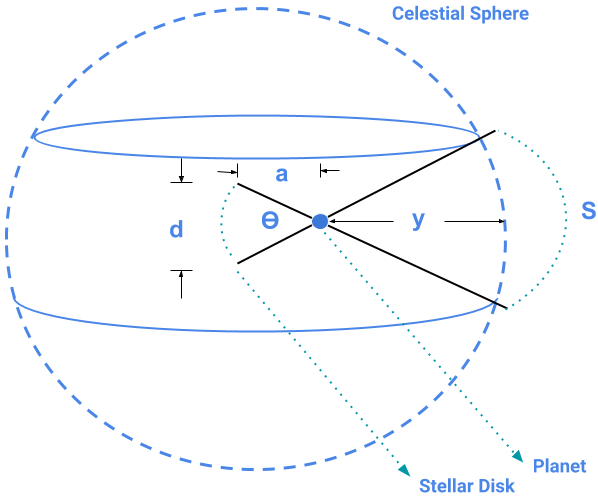
\includegraphics[width = 8cm, height = 7cm]{./Graficos/Capitulo_2/Illustrations/Prob_1.jpg}} 
\caption{\scriptsize{Geometry of the region swept out by the shadow of the planet during one orbital period on the celestial sphere. The planet is located at a distance $a$ from the parent star, and the stellar disk is assumed to have diameter $d_\star$}. In this particular case, the size of the planet is negligible. The total area swept out is projected onto the celestial sphere as represented by the strip cover by the angle $S$. The figure is inspired by \cauthor{1984Icar...58..121B} (\citeyear{1984Icar...58..121B}) work.}
\label{fig:Transit_1}
\end{figure}

In this case, the transit will not be produced by the point-like source but by its rings as a whole. This results in dips in the stellar flux revealing key system parameters. The geometry for this scenario is shown in \autoref{fig:Transit_2} where $R_\star$ is the stellar disk radius, $a$ represents the orbital semi-major axis and $R_H$ is the Hill sphere radius. The orbital inclination of $i = 0^\circ$ means the pole is on, whilst $i = 90^\circ$ means the equator is on. The transit can occur in two different ways:\\

\begin{enumerate}
\item Grazing transit $\textnormal{a} \cos \textnormal{i} \leq \textnormal{R}_\star + \textnormal{R}_\textnormal{H}$
\item Full transit $\textnormal{a} \cos \textnormal{i} \leq \textnormal{R}_\star - \textnormal{R}_\textnormal{H}$
\end{enumerate}

\begin{figure}[!ht]
\centering
  \subfloat{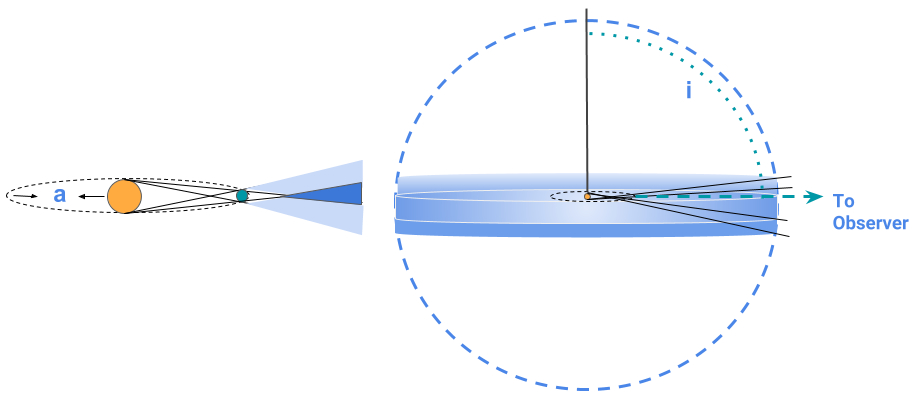
\includegraphics[width = 14cm, height = 6.2cm]{./Graficos/Capitulo_2/Illustrations/Prob_2.jpg}} 
\caption{\scriptsize{Geometry of the region swept out by the shadow of the planet during one orbital period on the celestial sphere. Though the planet is considered to have a negligible size, the Hill sphere where the rings are contained has a non-zero radius. The area swept out on the celestial sphere accounts for the inclination angle of the planet as seen by an observer located on the Earth. The figure is inspired by \cauthor{Cameron2016} (\citeyear{Cameron2016}) work.}}
\label{fig:Transit_2}
\end{figure}

In the absence of any prior knowledge of the system's inclination, the probability of transits being visible over interstellar distances is given by the fraction of the celestial sphere swept out by the planet's shadow as is shown in \autoref{fig:Transit_2} \cauthor{Cameron2016} (\citeyear{Cameron2016}). This is mainly dominated by the orbital inclination of the planet. Considering that the angle between the orbital inclination pole and the line of sight lies in a range ($i$, $i + \Delta i$), and it is randomly distributed as was assumed before, and also that transits occur only in nearly edge-on orbits i.e. $\textnormal{a} \cos \textnormal{i} \leq \textnormal{R}_\star + \textnormal{R}_\textnormal{H}$, we expect the probability to be uniform in $\mathrm{\cos \textnormal{i}}$ as shown in \autoref{fig:Transit_3}. Thus, the transit probability for randomly oriented orbits will be given by

\begingroup
\Large
\begin{equation}
\textnormal{P} \left( \cos \textnormal{i} < \frac{\textnormal{R}_\star + \textnormal{R}_\textnormal{H}}{\textnormal{a}} \right) = \frac{\textnormal{R}_\star + \textnormal{R}_\textnormal{H}}{\textnormal{a}}
 \label{eq:ProbTransit_4}
\end{equation}
\endgroup

\begin{figure}[!ht]
\centering
  \subfloat{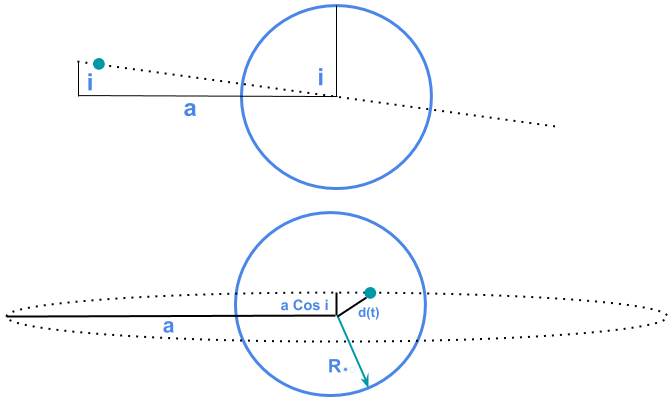
\includegraphics[width = 12cm, height = 7.3cm]{./Graficos/Capitulo_2/Illustrations/Prob_4.jpg}} 
\caption{\scriptsize{Geometry of the transit accounting for the inclination of the orbit. If $\textnormal{a} \cos \textnormal{i} \leq \textnormal{R}_\star + \textnormal{R}_\textnormal{H}$ the transit is grazing, while if $\textnormal{a} \cos \textnormal{i} \leq \textnormal{R}_\star - \textnormal{R}_\textnormal{H}$ the transit is full. As a random orientation of the orbit is considered the probability is uniform in ($\cos \textnormal{i}$) and reduces to the results shown in \autoref{eq:ProbTransit_4}}}
\label{fig:Transit_3}
\end{figure}

Then, in short, the transit probability of exoplanetary-rings in orbit around a given star where the orbital inclination is randomly distributed will be set by \autoref{eq:ProbTransit_4}, where we only need to consider the stellar and planet Hill sphere radii $R_\star$ and $R_H$ respectively, and the orbital semi-major axis. Apart from this, we need to care about when, and how long the rings can co-exist inside the Hill sphere of the planet. This probability was added at the end in order to study the overall change of what was assumed in \autoref{eq:Probabilities} and is presented in the next sub-section. 

\subsection{Rings Lifetime} \label{subsec:RingsSec}

It is well-known that the rings formation is a nonstatic phenomenon, and there is no privileged epoch in the formation of a planetary system when these features can form. On the other hand the only example, so far, we have to compare with, is our own solar system, making the statistical comparison quite hard in terms of deriving the exact formation conditions and time ranges. Nevertheless, simulations and current observations allow us to estimate the main processes that modify these structures, and give us a glimpse on their formation timescales.\\

Currently, most of the statistics are based on \textit{Hot Jupiters} \cauthor{2013pss3.book..309T} (\citeyear{2013pss3.book..309T}). However, there exist different problems with this, because the formation of rings around such objects can be affected by the low-obliquities causing the rings to edge-on or the small Hill sphere radius where they can be embedded in. In addition, viscous and Poynting-Robertson drags cause particle loss, and the high equilibrium black-body temperatures avoid materials to remain the solid state. Survival of the remnant ring depends on if they were created by tidal disruptions or continuous feeding because this will set the timescale on which the rings are expected to exist \cauthor{1984prin.conf..641H} (\citeyear{1984prin.conf..641H}). In our particular case, the most important question regarding the rings is: What is their age?. We need to know how long they are expected to live in order to properly compute the probability of observing ring systems around a planet given the overall age of the star and the planetary system itself. The age of the rings can be affected by the mean residence time of the particles on the rings or by how long the structure/sources have been in place For example in the case of Jupiter, if some moons suddenly disappear, or cease emitting dust, the rings will dissipate in $\sim 10^5$yr \cauthor{2013pss3.book..309T} (\citeyear{2013pss3.book..309T}). Interaction and physical processes may change or reset the age as can be the shepherding of the moons inside the rings leading to an age range of $100\times 10^6$-$6\times10^8$yr \cauthor{1994P&SS...42.1139C} (\citeyear{1994P&SS...42.1139C}), or ring's viscous spreading ($10^5$-$10^9$yr based on Saturn's ring A) \cauthor{2009sfch.book..537C} (\citeyear{2009sfch.book..537C}) or ($\sim10^9$yr) from viscous timescales if the gas is considered to be non-turbulent \cauthor{1984prin.conf..641H} (\citeyear{1984prin.conf..641H}). There is also a chance that the ring is completely disrupted (based on the fragmentation criteria), so in that case we end up with a timescale for complete loss of the rings of $10^{7}$-$10^8$yr \cauthor{1994P&SS...42.1139C} (\citeyear{1994P&SS...42.1139C}) or based on evolutionary processes $< 10^8$yr \cauthor{2009sfch.book..537C} (\citeyear{2009sfch.book..537C}). On the other hand, considering cometary passages which could break a satellite or to tidally disrupt the comet applied to Saturn's ring lead to a time range of $10^7$-$10^8$yr for the A-ring, $10^8$-$10^9$yr for the B-ring, and $10^7$yr from radial spreading \cauthor{2009sfch.book..537C} (\citeyear{2009sfch.book..537C}).\\

As has been presented above, different age ranges can be derived for the rings lifetime through models and observations of our own solar system. However, the remaining question is: Do they form at the very beginning, in the middle or at the end of the planetary system formation?. According to \cauthor{2009Icar..199..413C} (\citeyear{2009Icar..199..413C}) the main core of Saturn's B-ring was formed in the first Gyr of the solar system in which collisions are expected to be much more likely. However, from simulations it is pointed out Saturn's ring formation can be understood a huge disruption near the end of the planetary formation period during which the circum-planetary gas disk is still present \cauthor{2010Natur.468..943C} (\citeyear{2010Natur.468..943C}). If we look to Uranus or Neptune, possibly they have been less affected and have not changed dramatically over the age of the solar system, where rings and moons have been oscillating between accretion and disruption for many Gyr \cauthor{2013pss3.book..309T} (\citeyear{2013pss3.book..309T}).\\

In general, there is no complete consensus on whether the rings form at the beginning, or at the end of the planetary formation process, neither on the time they can live as a ringed-structure around the planet. Base on this, we decided to introduce a fifth probability to account for the most likely lifespan a ring can have. The probability is defined in \autoref{eq:Prob_5}, but it is necessary to have in mind that as it is hard to guarantee the exact moment in time where they form, then this probability assumes each time interval has the same chance and we can only provide an estimation based on the mean-rings lifespan as a function of the stellar age.  

\begingroup
\Large
\begin{equation}
\textnormal{P}_5 = \frac{\textnormal{Rings}~\textnormal{lifespan}}{\textnormal{Host}~\textnormal{star's}~\textnormal{age}}
 \label{eq:Prob_5}
\end{equation}
\endgroup

%============================================================================================================================================================

\section{Monte-Carlo simulations} \label{sec:MCSec}

As was shown in \autoref{sec:PowerLawSec}, we have two different ways to generate the exoplanetary mass-period distribution either by considering a weak correlation e.g. $\beta$-distribution or using a simple power law derived from the observations. One way or another, we are able to generate a new sample of planets with mass and period following a given distribution using the Monte-Carlo method. This method consists in drawing a sample of $N$ values which follows the wanted distribution using randomly distributed numbers.\\

%In the first case, we have the $\beta$-distribution addressed in \autoref{subsec:BetaDist}. A sample of $10.000$ mass-period pairs were generated following \autoref{eq:Beta_Monte}, where ($\alpha_\textnormal{m}, \beta_\textnormal{m}$), ($\alpha_\textnormal{p}, \beta_\textnormal{p}$), and ($\delta_\textnormal{1}, \delta_\textnormal{2}$) were created using pseudo-random numbers following a $\beta$-distribution as mentioned in \cauthor{1538-3881-134-5-2061} \citeyear{1538-3881-134-5-2061}. The mass and period range covers $0.008 \leq \textnormal{m/Mj} \leq 26.7$, and $0.8079 \leq \textnormal{p/days} \leq 6776.1$ respectively.\\

% \begingroup
% \Large
% \begin{equation}
%   \begin{align*}
%   \textnormal{m}~~&=~~155.5*(\alpha_\textnormal{m} + \delta_\textnormal{1}) / (\alpha_\textnormal{m} + \delta_\textnormal{1} + \beta_\textnormal{m} + \delta_\textnormal{2}) \\[10pt]
%   \textnormal{p}~~&=~~11650.0*(\alpha_\textnormal{p} + \delta_\textnormal{1}) / (\alpha_\textnormal{p} + \delta_\textnormal{1} + \beta_\textnormal{p} + \delta_\textnormal{2})
%  \label{eq:Beta_Monte}
%  \end{align*}
% \end{equation}
% \endgroup \\

%The period/mass, period/semi-major axis, and mass/semi-major axis are shown in figures \autoref{fig:PeriodMass_Beta},\autoref{fig:PeriodMajor_Beta}, and  \autoref{fig:MassMajor_Beta} respectively where each dot corresponds to each pair generated using the $\beta$-distribution method, and the semi-major axis was computed using Kepler's third law.\\ 


% \begin{figure}[!ht]
% \centering
%   \subfloat{\includegraphics[width = 12cm, height = 9cm]{./Graficos/Capitulo_2/2_Exop_distributions/Period_mass_distribution_2.png}} 
% \caption{\scriptsize{Exoplanetary period (days) as a function of exoplanetary mass ($\textnormal{Mj}$). Each value corresponds to a planetary mass-period pair generated following the $\beta$-distribution approach as mentioned in \cauthor{1538-3881-134-5-2061} \citeyear{1538-3881-134-5-2061} using a Monte-Carlo simulation of $10.000$ objects. The majority of planets tend to aggregate around the small period and mass values.}}
% \label{fig:PeriodMass_Beta}
% \end{figure}
% 
% \begin{figure}[!ht]
% \centering
%   \subfloat{\includegraphics[width = 12cm, height = 9cm]{./Graficos/Capitulo_2/2_Exop_distributions/Period_major_distribution_2.png}} 
% \caption{\scriptsize{Exoplanetary period (days) as a function of semi-major axis ($\textnormal{AU}$). Each value corresponds to a planetary mass-period pair generated following the $\beta$-distribution approach as mentioned in \cauthor{1538-3881-134-5-2061} \citeyear{1538-3881-134-5-2061} using a Monte-Carlo simulation of $10.000$ objects. The semi-major axis was derived using Kepler's third law which sets the left-and right boundaries of the distribution. Planets beyond $\textnormal{a} \approx 20 \textnormal{AU}$ cannot be generated due to the period-mass ranges evaluated.}}
% \label{fig:PeriodMajor_Beta}
% \end{figure}
% 
% \begin{figure}[!ht]
% \centering
%   \subfloat{\includegraphics[width = 12cm, height = 9cm]{./Graficos/Capitulo_2/2_Exop_distributions/Mass_major_distribution_2.png}} 
% \caption{\scriptsize{Exoplanetary mass ($\textnormal{Mj}$) as a function of semi-major axis ($\textnormal{AU}$). Each value corresponds to a planetary mass-period pair generated following the $\beta$-distribution approach as mentioned in \cauthor{1538-3881-134-5-2061} \citeyear{1538-3881-134-5-2061} using a Monte-Carlo simulation of $10.000$ objects. The semi-major axis was derived using Kepler's third law which sets the left-and right boundaries of the distribution. Planets beyond $\textnormal{a} \approx 20 \textnormal{AU}$ cannot be generated due to the period-mass ranges evaluated.}}
% \label{fig:MassMajor_Beta}
% \end{figure}

We decided to use the single power law approach as suggested by (\cauthor{2008PASP..120..531C} \citeyear{2008PASP..120..531C}; \cauthor{2006ApJ...646..505B} \citeyear{2006ApJ...646..505B}) to generate the mass-period distribution for exoplanets, and also following the well-known Salpeter- and-Kroupa's power law to generate the stellar masses as was explained in \autoref{subsec:Salpeter} and \autoref{subsec:Kroupa} individually. Following this method, we set the values for the exponents in the case of the exoplanets to $1.16$ and $0.74$ for the mass and the period respectively as suggested in \cauthor{2010EAS....41..107N} (\citeyear{2010EAS....41..107N}) who basically based his results on different observations and corrections to values previously obtained by \cauthor{2008PASP..120..531C} (\citeyear{2008PASP..120..531C}) and \cauthor{2006ApJ...646..505B} (\citeyear{2006ApJ...646..505B}). According to the last, we can generate a sample of exoplanetary masses and periods in a range covering $0.3 \leq \textnormal{m/Mj} \leq 10$, and $2 \leq \textnormal{p/days} \leq 2000$. Thus, a sample of $10.000$ pairs was drew following the method explained in \autoref{sec:PowerLawSec}. In \autoref{fig:Mass_Nielsen} and \autoref{fig:Period_Nielsen} the histogram and the cumulative function for the generated values are shown in blue whilst the orange dashed line shows the expected shape that these values should follow from the original power law. The figures on the left are shown in linear scale while those on the right are in logarithmic scale. It is clear that both, the mass and period values simulated follow the original power law. Same process was performed using the $\beta$-distribution but the final results were not so different. For comparison the period/mass, period/semi-major axis, and mass/semi-major axis are shown in figures \autoref{fig:PeriodMass_Nielsen},\autoref{fig:PeriodMajor_Nielsen}, and  \autoref{fig:MassMajor_Nielsen} respectively. However, as using the power law we can double check that the simulated values follow the original trend, which is not the case for the $\beta$-distribution where the constants are imposed from their observations, we decided use the power-law method to generate our final sample of mass-period pairs.\\ 

\begin{figure}[!ht]
\centering
  \subfloat{\includegraphics[width = 18.5cm, height = 15.5cm, scale = 1.0, angle = 90]{./Graficos/Capitulo_2/2_Exop_distributions/Mass_distribution_Nielsen.png}} 
\caption{\scriptsize{Monte-Carlo simulation of exoplanetary mass distribution following a power law of slope $1.16$ \cauthor{2010EAS....41..107N} (\citeyear{2010EAS....41..107N}). \textit{\textbf{Top-Left}}: histogram corresponding to the $10.000$ masses generated using the Monte-Carlo approach. The orange line represents the analytic shape the distribution should follow. \textit{\textbf{Top-Right}}: same as figure described in \textit{Top-Left} but using logarithmic x-scale for comparison. \textit{\textbf{Bottom-Left}}: cumulative mass distribution function for the generated masses is shown in blue while the analytic is shown in orange. \textit{\textbf{Bottom-Right}}: same as described in \textit{Bottom-Left} but using logarithmic-scales. The feature produced at low mass values which makes both curves differ because the minimum simulated value is slightly above the possible minimum mass.%The feature produced at low mass values which makes both curves differ is an artifact of the logarithmic-scale and it does not correspond to a real deviation in the simulated data.
}}
\label{fig:Mass_Nielsen}
\end{figure}

\begin{figure}[!ht]
\centering
  \subfloat{\includegraphics[width = 18.5cm, height = 15.5cm, scale = 1.0, angle = 90]{./Graficos/Capitulo_2/2_Exop_distributions/Period_distribution_Nielsen.png}} 
\caption{\scriptsize{Monte-Carlo simulation of exoplanetary period distribution following a power law of slope $0.74$ \cauthor{2010EAS....41..107N} (\citeyear{2010EAS....41..107N}). \textit{\textbf{Top-Left}}: histogram corresponding to the $10.000$ periods generated using the Monte-Carlo approach. The orange line represents the analytic shape the distribution should follow. \textit{Top-Right}: same as figure described in \textit{Top-Left} but using logarithmic x-scale for comparison. \textit{\textbf{Bottom-Left}}: cumulative mass distribution function for the generated masses is shown in blue while the analytic is shown in orange. \textit{\textbf{Bottom-Right}}: same as described in \textit{\textbf{Bottom-Left}} but using logarithmic-scales. The feature produced at low mass values which makes both curves differ because the minimum simulated value is slightly above the possible minimum mass.%The feature produced at low mass values which makes both curves differ is an artifact of the logarithmic-scale and it does not correspond to a real deviation in the simulated data.
}}
\label{fig:Period_Nielsen}
\end{figure}

\begin{figure}[!ht]
\centering
  \subfloat{\includegraphics[width = 12cm, height = 9cm]{./Graficos/Capitulo_2/2_Exop_distributions/Period_mass_distribution.png}} 
\caption{\scriptsize{Exoplanetary period (days) as a function of exoplanetary mass ($\textnormal{Mj}$). Each value corresponds to a planetary mass-period pair generated following power-law distribution approach as mentioned in \cauthor{2010EAS....41..107N} (\citeyear{2010EAS....41..107N}) using a Monte-Carlo simulation of $10.000$ objects. The majority of planets tend to aggregate around the small period and mass values. %In comparison to \autoref{fig:PeriodMass_Beta}, the period-range is smaller, but the general trend is kept.
}}
\label{fig:PeriodMass_Nielsen}
\end{figure}

\begin{figure}[!ht]
\centering
  \subfloat{\includegraphics[width = 12cm, height = 9cm]{./Graficos/Capitulo_2/2_Exop_distributions/Period_major_distribution.png}} 
\caption{\scriptsize{Exoplanetary period (days) as a function of semi-major axis ($\textnormal{AU}$). Each value corresponds to a planetary mass-period pair generated following power-law distribution approach as mentioned in \cauthor{2010EAS....41..107N} (\citeyear{2010EAS....41..107N}) using a Monte-Carlo simulation of $10.000$ objects. The semi-major axis was derived using Kepler's third law which sets the left-and right boundaries of the distribution. %In comparison to \autoref{fig:PeriodMajor_Beta}, planets beyond $\textnormal{a} \approx 7 \textnormal{AU}$ cannot be generated due to the period-mass ranges evaluated.
}}
\label{fig:PeriodMajor_Nielsen}
\end{figure}

\begin{figure}[!ht]
\centering
  \subfloat{\includegraphics[width = 12cm, height = 9cm]{./Graficos/Capitulo_2/2_Exop_distributions/Mass_major_distribution.png}} 
\caption{\scriptsize{Exoplanetary mass ($\textnormal{Mj}$) as a function of semi-major axis ($\textnormal{AU}$). Each value corresponds to a planetary mass-period pair generated power-law distribution approach as mentioned in \cauthor{2010EAS....41..107N} (\citeyear{2010EAS....41..107N}) using a Monte-Carlo simulation of $10.000$ objects. The semi-major axis was derived using Kepler's third law which sets the left-and right boundaries of the distribution. %In comparison to \autoref{fig:MassMajor_Beta}, planets beyond $\textnormal{a} \approx 7 \textnormal{AU}$ cannot be generated due to the period-mass ranges evaluated.
}}
\label{fig:MassMajor_Nielsen}
\end{figure}

Finally, the same power-law method was used to generate the stellar mass. As was introduced in \autoref{subsec:Salpeter} and \autoref{subsec:Kroupa}, we have two different power laws which can describe the stellar mass functions. Taking into account that in general there is no consensus on a single exponent which could describe the distribution of stellar masses in the universe, we decided to test both exponents but paying more attention to the Kroupa's initial mass function distribution because we think it is a more realistic description of the stellar IMF. Following this, we created once again a sample of $10.000$ stars following the initial mass function described by a Salpeter's and Kroupa's exponent. In the case of Salpeter, the mass range covers  $0.1 \leq \textnormal{m/M$_\odot$} \leq 10$ with an exponent of $2.35$, whilst the Kroupa's range covers $0.1 \leq \textnormal{m/M$_\odot$} \leq 0.5$ with an exponent of $1.3$, and an exponent of $2.3$ for $0.5 \leq \textnormal{m/M$_\odot$} \leq 10$. The drawn distributions are shown in \autoref{fig:Salpeter_IMF} and \autoref{fig:Kroupa_IMF}, where the histogram and cumulative functions are shown in blue and the original power law distributions are shown with the dashed orange line. In the case of the Kroupa's distribution, a fine break can be seen in the logarithmic scale figure for the small stellar masses due to the fact that we are using two different exponents for different mass ranges.\\  

\begin{figure}[!ht]
\centering
  \subfloat{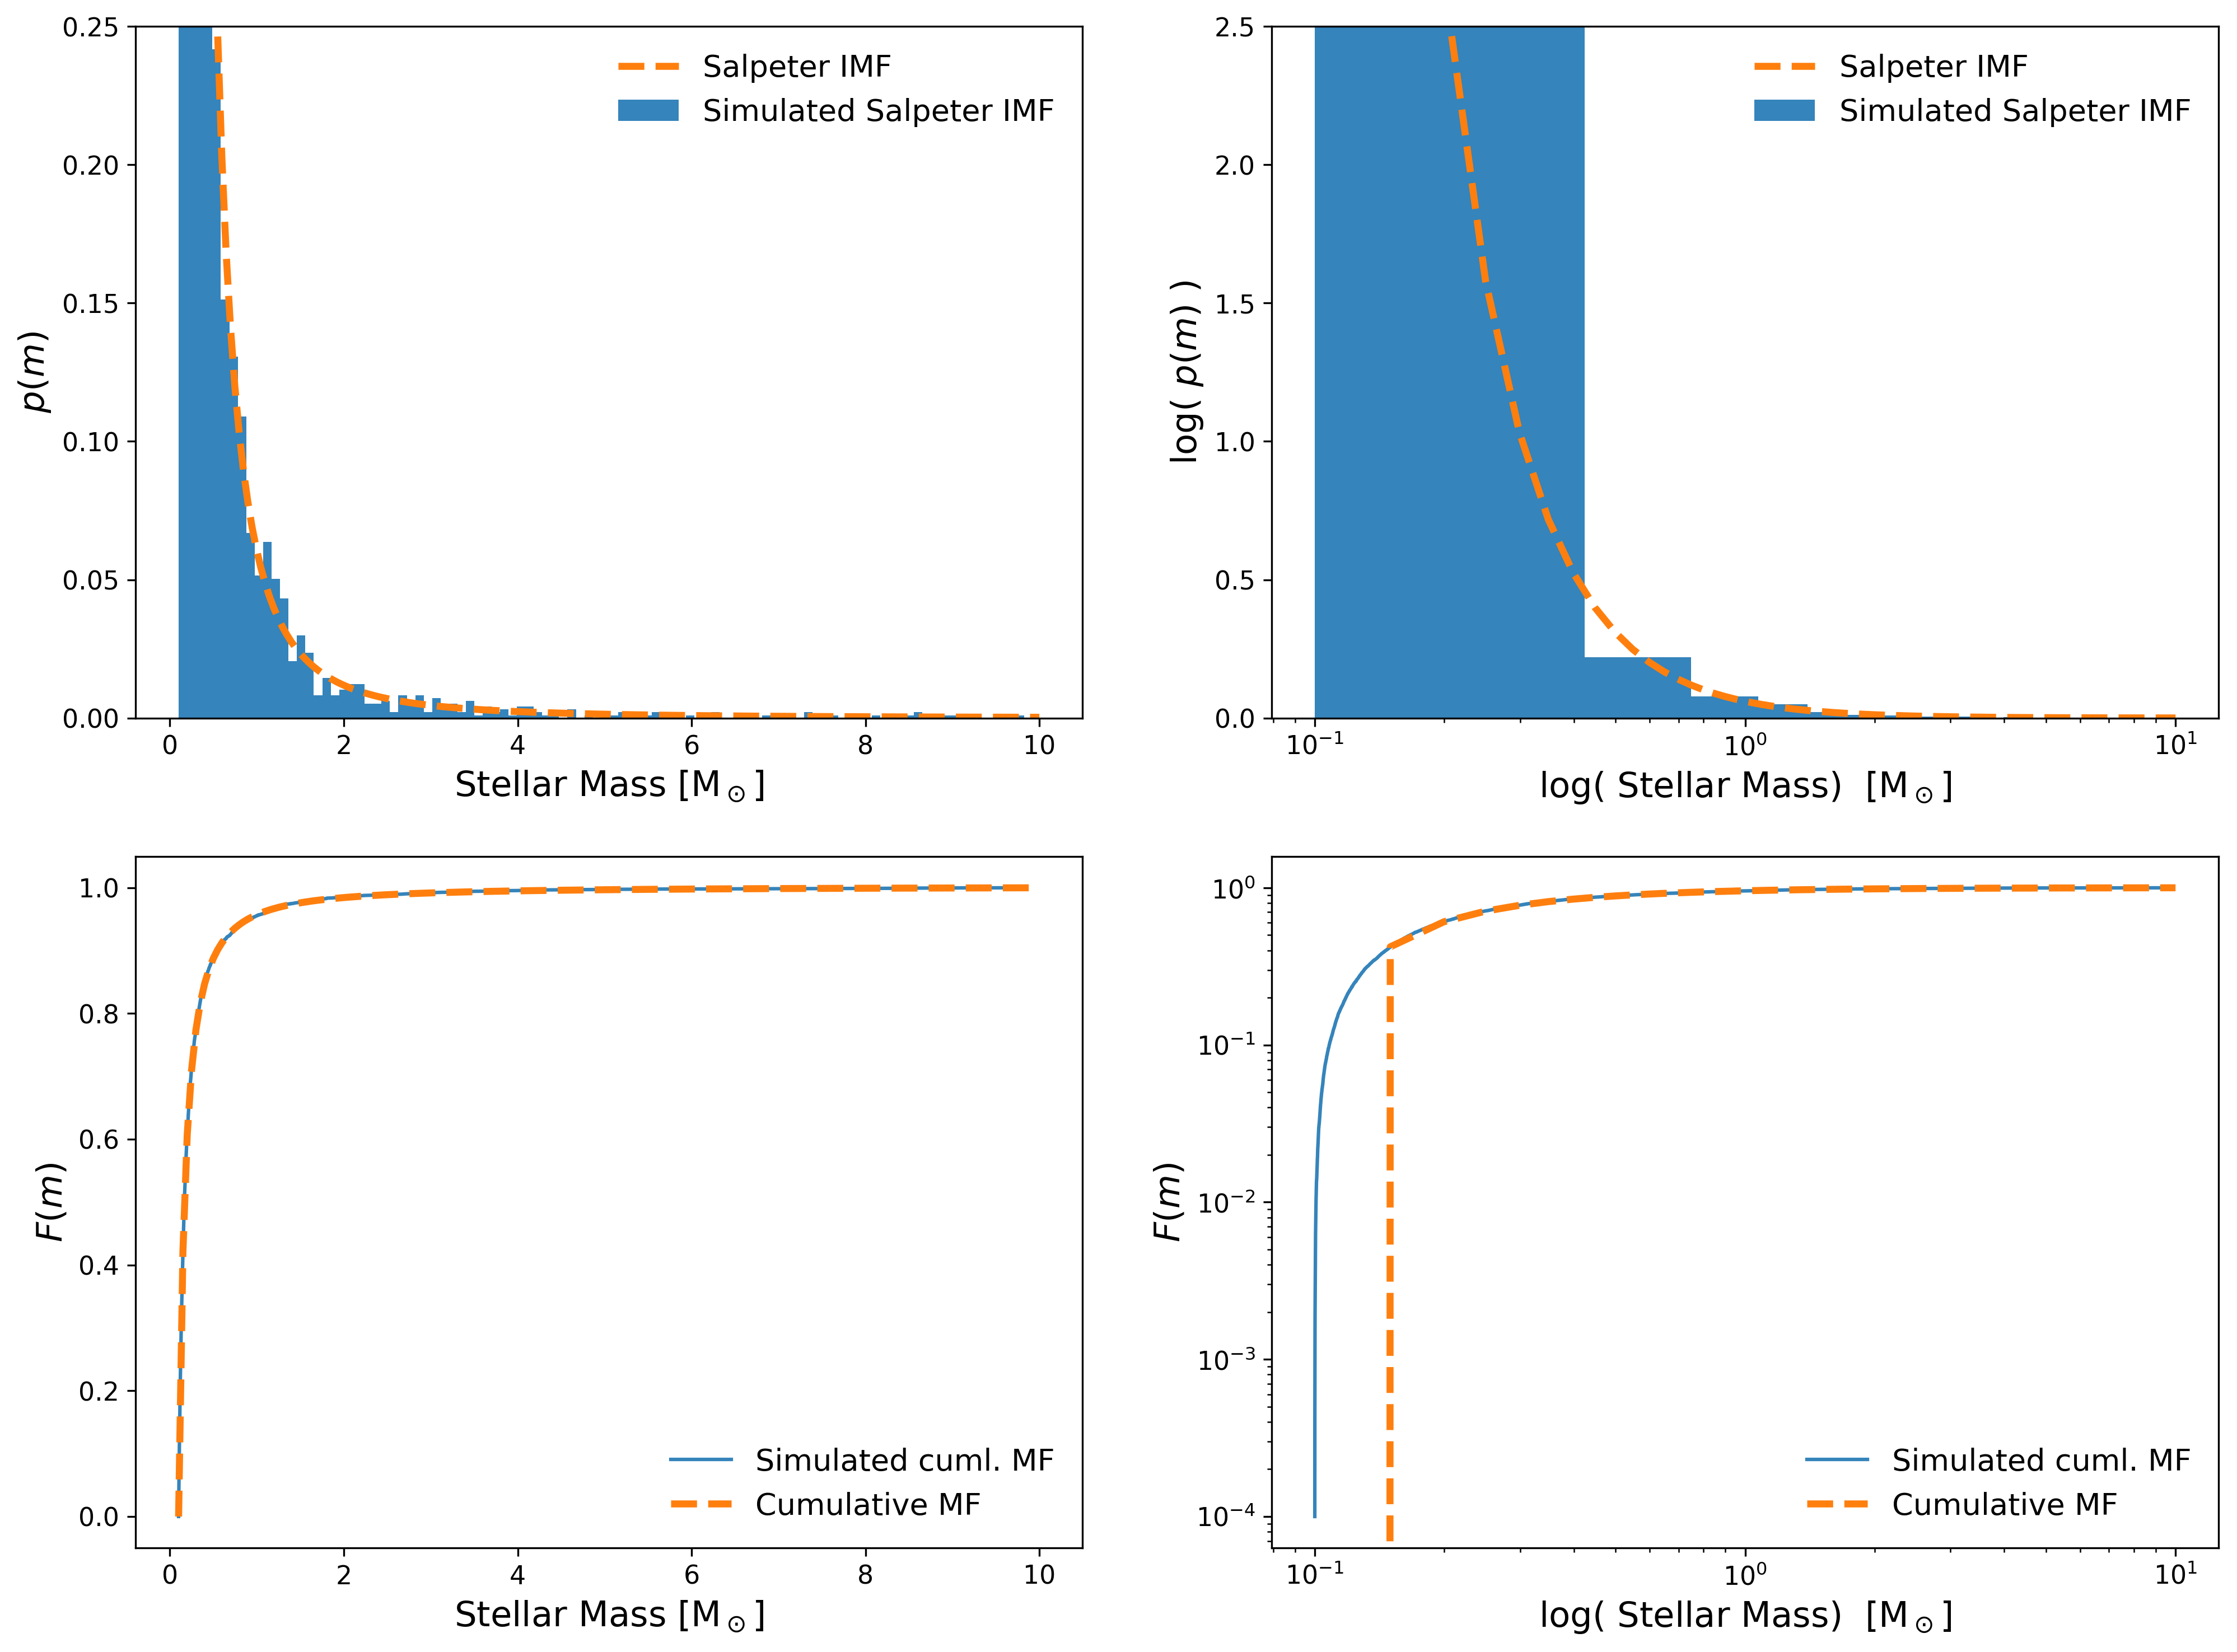
\includegraphics[width = 18.5cm, height = 15.5cm, scale = 1.0, angle = 90]{./Graficos/Capitulo_2/2_Exop_distributions/Salpeter.png}} 
\caption{\scriptsize{Monte-Carlo simulation of stellar mass distribution following a Salpeter's power law. \textit{\textbf{Top-Left}}: histogram corresponding to the $10.000$ stellar masses generated using the Monte-Carlo approach. The orange line represents the analytic shape the distribution should follow. \textit{\textbf{Top-Right}}: same as figure described in \textit{Top-Left} but using logarithmic x-scale for comparison. \textit{\textbf{Bottom-Left}}: cumulative stellar mass distribution function for the generated masses is shown in blue while the analytic is shown in orange. \textit{Bottom-Right}: same as described in \textit{\textbf{Bottom-Left}} but using logarithmic-scales. The feature produced at low mass values which makes both curves differ because the minimum simulated date is slightly above the possible minimum mass.%The feature produced at low mass values which makes both curves differ is an artifact of the logarithmic-scale and it does not correspond to a real deviation in the simulated data.
}}
\label{fig:Salpeter_IMF}
\end{figure}

\begin{figure}[!ht]
\centering
  \subfloat{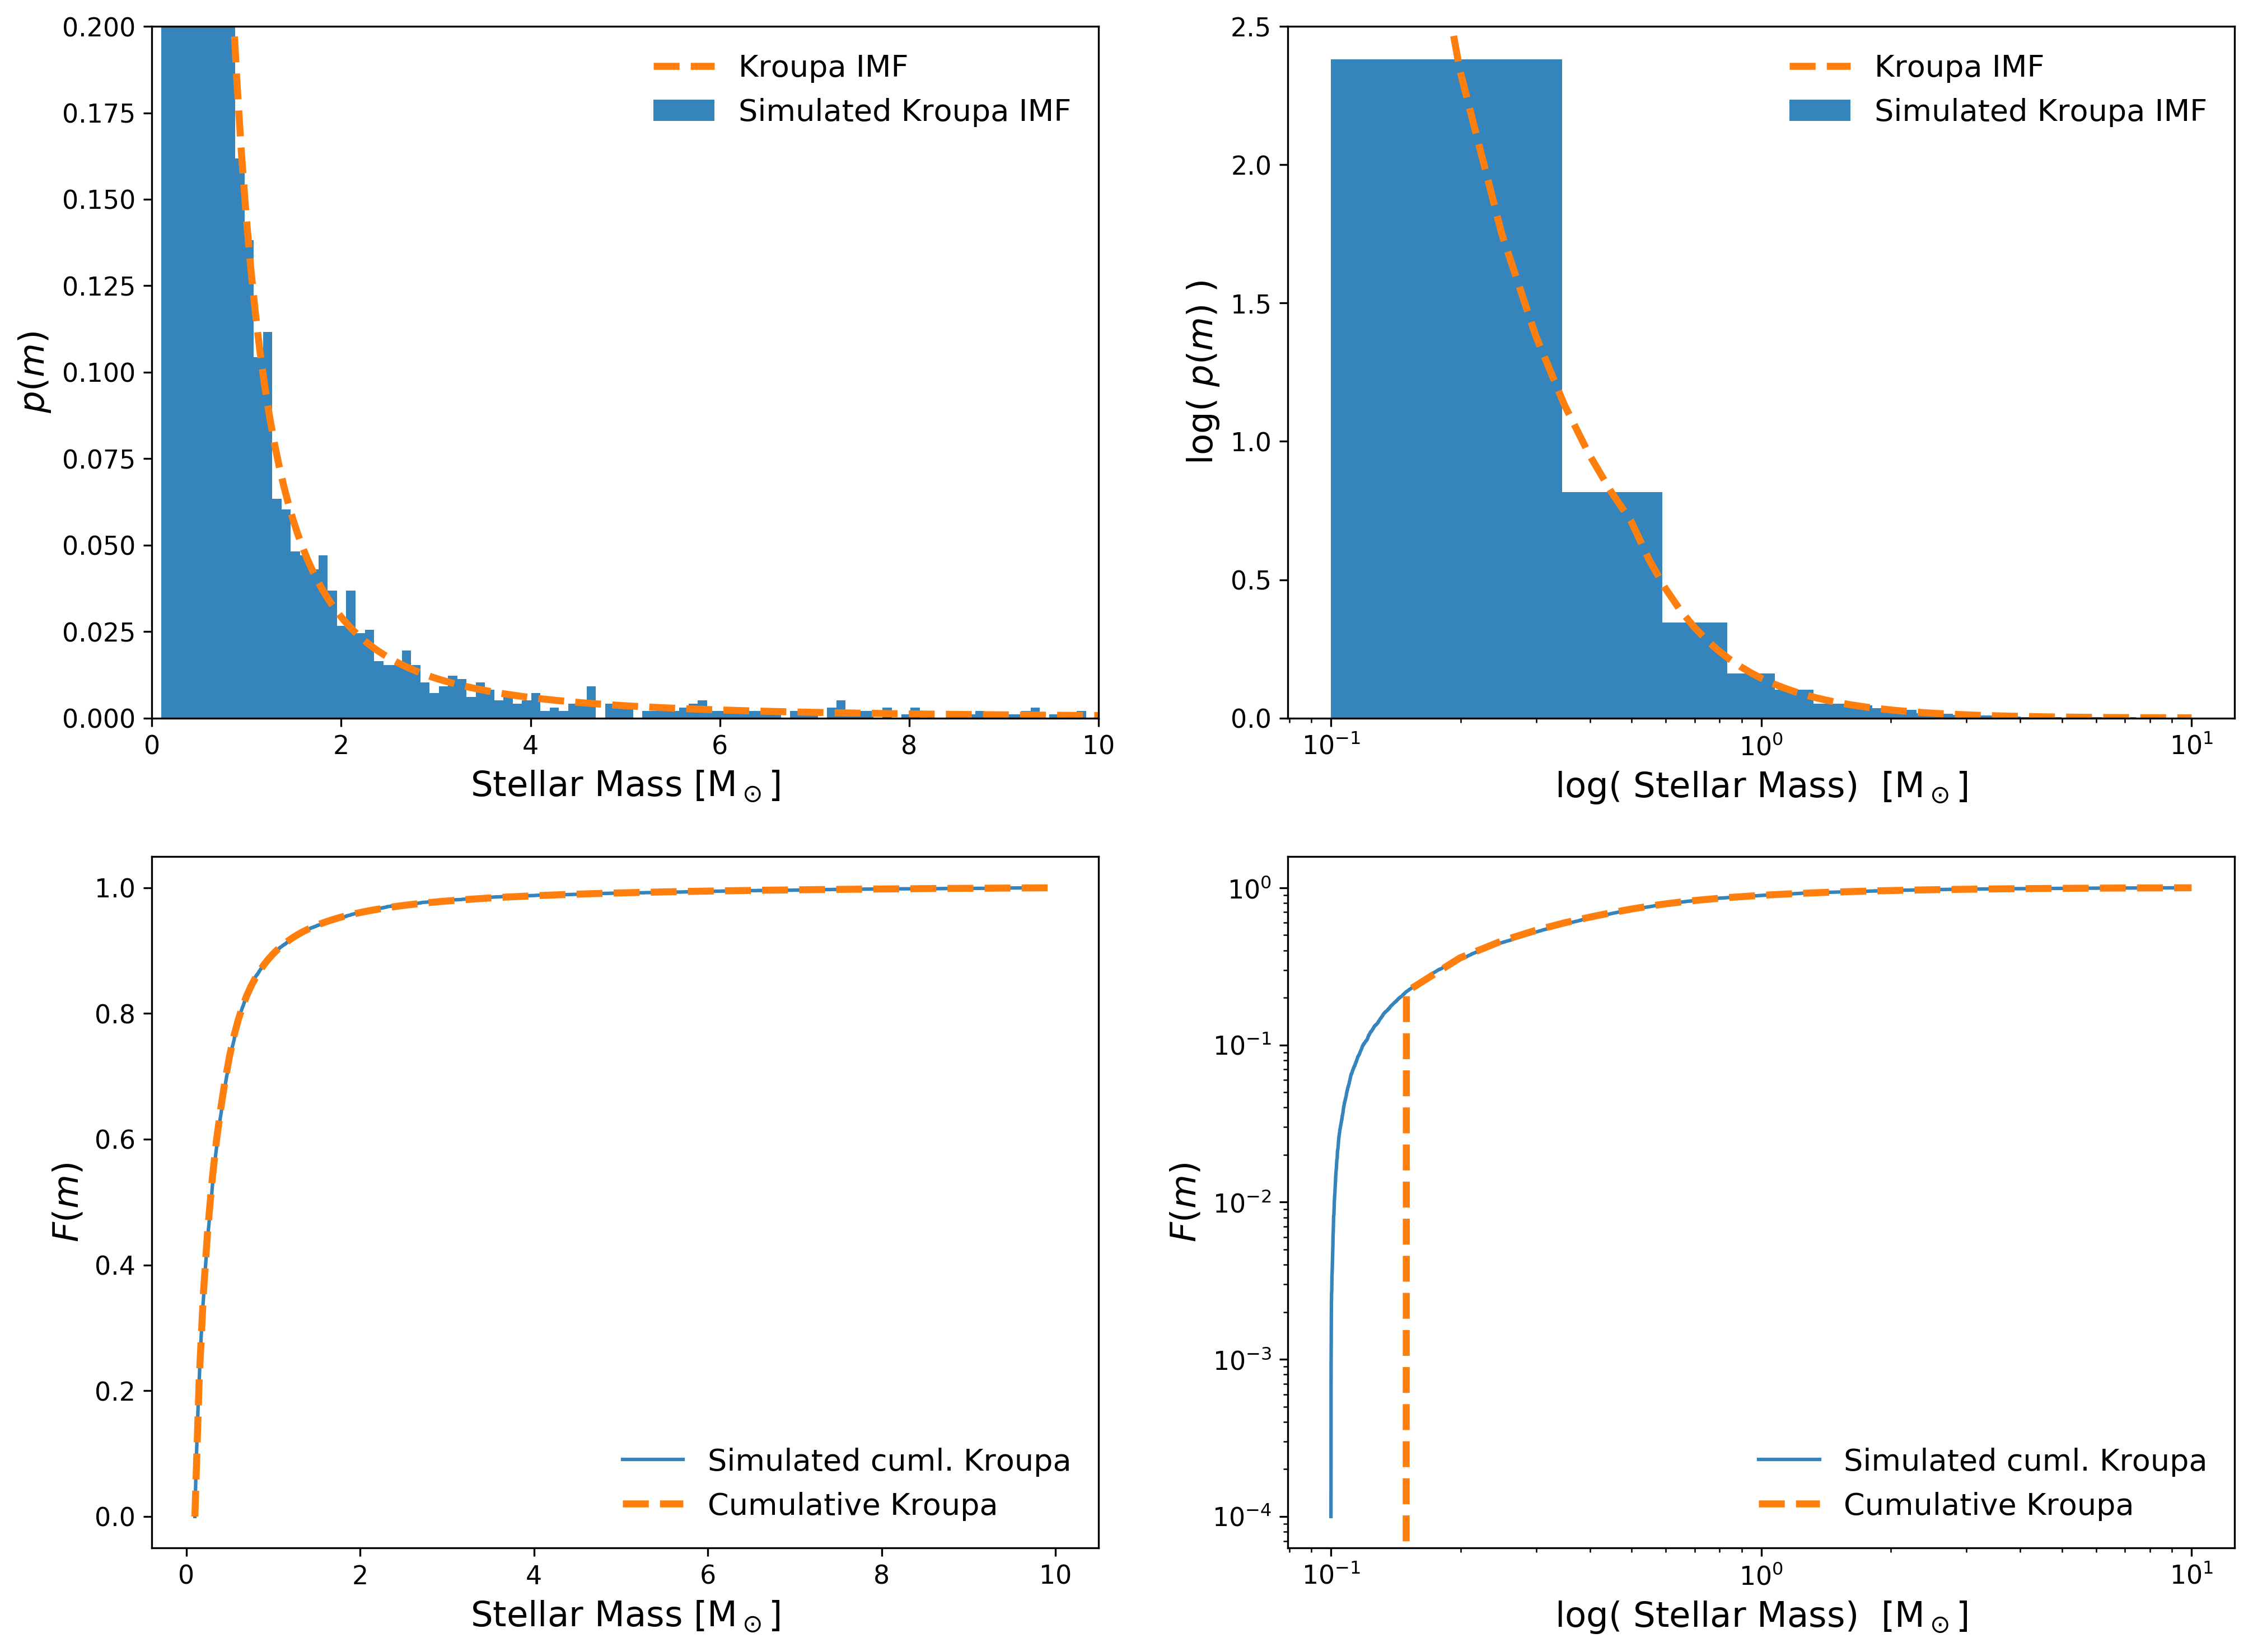
\includegraphics[width = 18.5cm, height = 15.5cm, scale = 1.0, angle = 90]{./Graficos/Capitulo_2/2_Exop_distributions/Kroupa.png}} 
\caption{\scriptsize{Monte-Carlo simulation of stellar mass distribution following a Kroupa's power law. \textit{\textbf{Top-Left}}: histogram corresponding to the $10.000$ stellar masses generated using the Monte-Carlo approach. The orange line represents the analytic shape the distribution should follow. \textit{\textbf{Top-Right}}: same as figure described in \textit{Top-Left} but using logarithmic x-scale for comparison. \textit{\textbf{Bottom-Left}}: cumulative stellar mass distribution function for the generated masses is shown in blue while the analytic is shown in orange. \textit{Bottom-Right}: same as described in \textit{\textbf{Bottom-Left}} but using logarithmic-scales. The feature produced at low mass values which makes both curves differ because the minimum simulated date is slightly above the possible minimum mass.%The feature produced at low mass values which makes both curves differ is an artifact of the logarithmic-scale and it does not correspond to a real deviation in the simulated data.
}}
\label{fig:Kroupa_IMF}
\end{figure}

Summarizing, we generated a sample of $10.000$ exoplanetary mass-period pairs and stellar masses individually following in the case of the exoplanets $\beta$-distribution or a simple power law, and in the case of the stellar initial mass function using two different power laws known as Salpeter's and Kroupa's initial mass function. As we have different ways to generate mock samples, we decided to stick to the power law generation in the case of the exoplanetary mass-period distribution because we are able to check the cumulative function and check if the currently drawn pairs follow the original distributions. In the same way, for the stellar mass generation, we decided to use the Kroupa's distribution because is more general. Having said this, we proceed to use these values and the previous information presented in the last sections to compute the probability of transit detection. This is thoroughly explained in \autoref{sec:AnalyticForm} in which we address this calculation in two different ways. Firstly, using the results from the Monte-Carlo simulations, and secondly evaluating directly the analytic form of the transit probability.     


%============================================================================================================================================================

\section{Detection Probability: Monte-Carlo vs Analytic Form} \label{sec:AnalyticForm}
%============================================================================================================================================================

In \autoref{sec:DetectionProbability}, the main components of the probability of a ringed-system transiting in front of its parent star was addressed. However, the main goal is to constrain for the different exoplanetary mass-period pairs, how this probability changes as a function of the stellar mass. We decided to tackle down this problem in two different ways: i) using the Monte-Carlo results for the exoplanetary mass-period distributions, and ii) simply generating the probability from the analytic form without recurring to any Monte-Carlo generation of values. In both cases, we use the probability function shown in \autoref{eq:FinalDetectProb} which does not include the fifth probability corresponding to the planetary rings' lifetime. This will be addressed separately at the end of this section.\\

First of all, in the case of the Monte-Carlo process, a sample of $10.000$ stars between $0.1 \leq \textnormal{m/M$_\odot$} \leq 10.0$ was generated following the Kroupa's initial mass function. Moreover, a sample of $10.000$ mass-period pairs was also generated following the power law distribution suggested by \cauthor{2010EAS....41..107N} (\citeyear{2010EAS....41..107N}) and explained in \autoref{sec:MCSec}. Once we have set the final sample of exoplanets and stars to be tested, we proceed to evaluate out the detection probability function which is given by \autoref{eq:FinalDetectProb}. It is important to have in mind that in this equation the values corresponding to the exoplanetary mass and period are taken from the Monte-Carlo simulation. Also, the semi-major axis is obtained using Kepler's third law, and the stellar mass is obtained with the Monte-Carlo generation as well. We need to have a relationship between the stellar masses and stellar radii. To achieve this goal, we used two different approaches. The first one assumes that the stars are in the main sequence and follow the regular relation given by $\textnormal{R} \propto \textnormal{M}^{0.8}$. However, this assumes that the stars are already in the ZAMS, have the solar metallicity and are massive stars burning H to He via the CNO chain. This not entirely true for our purposes because we aim to study young stellar populations. Thus, we decided to use the \textit{MESA}-code provided through the \textit{MIST}-package (\cauthor{2016ApJS..222....8D} \citeyear{2016ApJS..222....8D}; \cauthor{2016ApJ...823..102C} \citeyear{2016ApJ...823..102C}) to compute the stellar isochrone for a $20Myr$ star varying the masses between $0.1 \leq \textnormal{m/M$_\odot$} \leq 10.0$ which is the range we are interested in. In \autoref{fig:RMInterpol}, the stellar radius versus the stellar mass obtained using the $20Myr$ isochrone is shown. The blue dots correspond to the values retrieved by the model while the orange dots represent a linear interpolation performed to complete some empty regions in the isochrone. Once this is settled, we can assign the expected stellar radius for a given mass assuming that the stellar age is close to $20Myr$.\\ 

\begingroup
\large
\begin{equation}
  \textnormal{Detection Probability} = 0.17 \left(\frac{\textnormal{R}_\star + \textnormal{R}_\textnormal{H}}{\textnormal{a}} \right) \left[ 1 - \left( \frac{\textnormal{Gaia}~\textnormal{Duration} - \textnormal{Eclipse}~\textnormal{Duration}}{\textnormal{Gaia}~\textnormal{Duration}} \right)^\textnormal{n} \right]
 \label{eq:FinalDetectProb}
\end{equation}
\endgroup \\

\begin{figure}[!ht]
\centering
  \subfloat{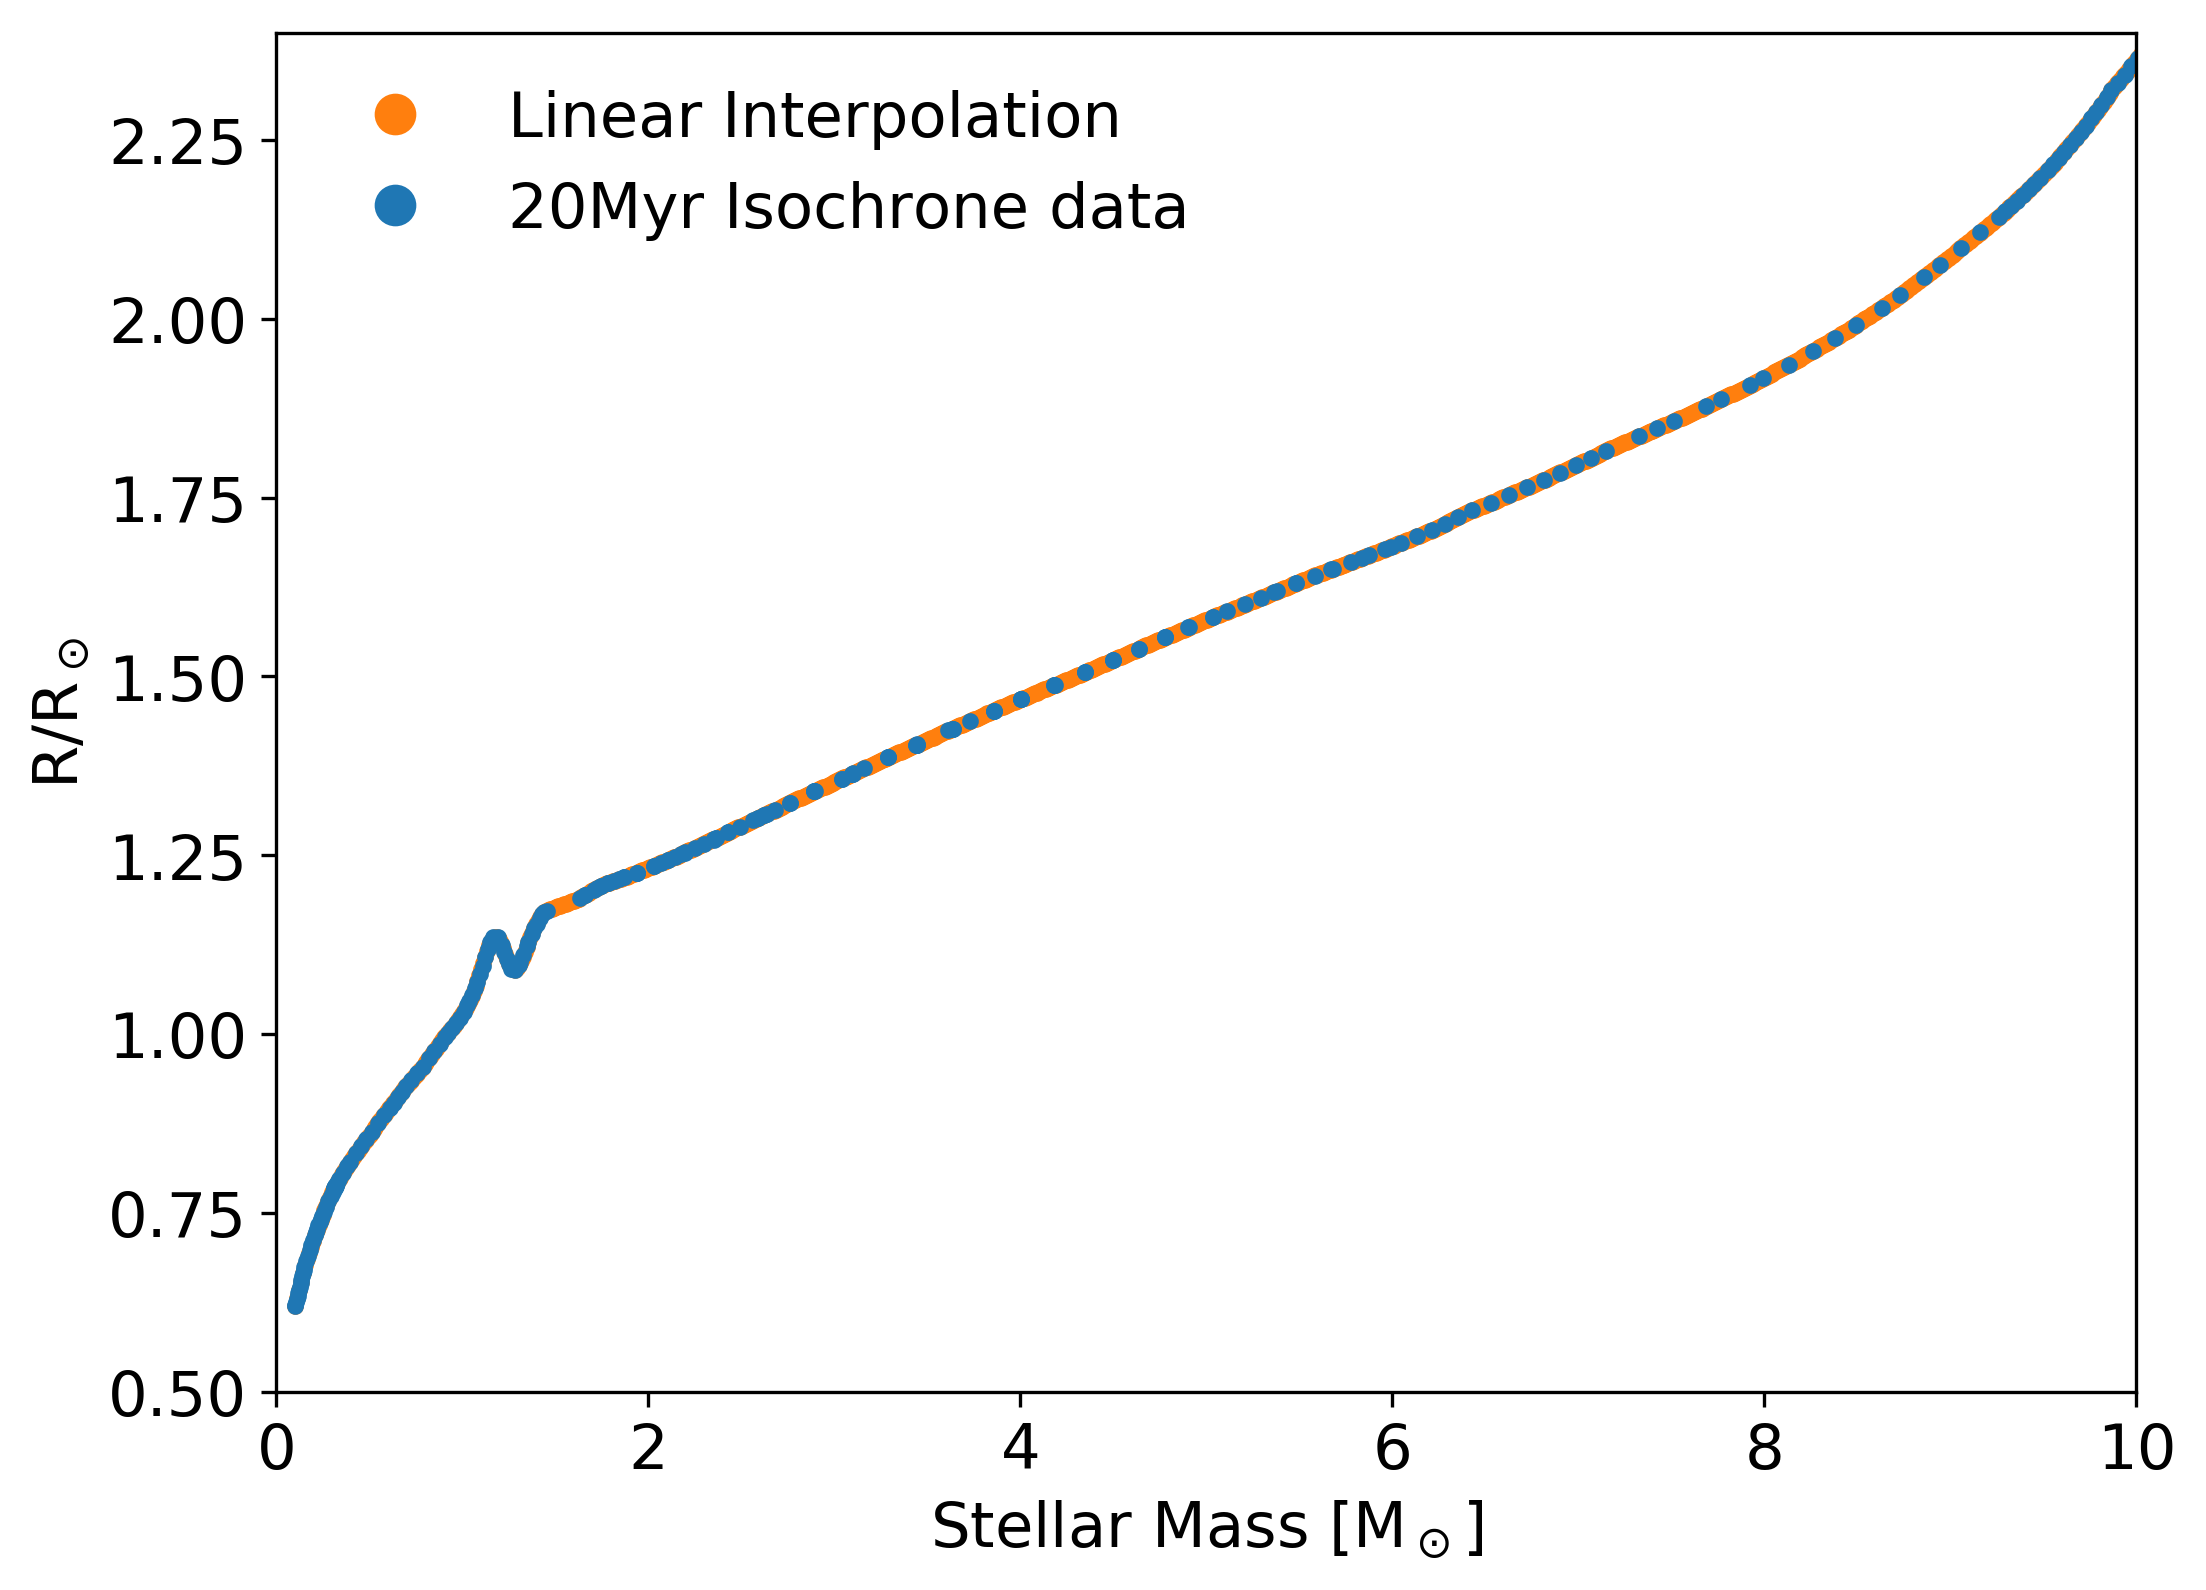
\includegraphics[width = 12cm, height = 9cm]{./Graficos/Capitulo_2/2_Exop_distributions/Linear_Interpolation.png}} 
\caption{\scriptsize{Linear interpolation of a $20 \textnormal{Myr}$ isochrone stellar radius as a function of mass. The blue dots correspond to the stellar radius as a function of stellar mass for a $20 \textnormal{Myr}$ isochrone calculated using the \textit{MIST}-package (\cauthor{2016ApJS..222....8D} \citeyear{2016ApJS..222....8D}; \cauthor{2016ApJ...823..102C} \citeyear{2016ApJ...823..102C}). The orange dots are the result of the linear interpolation performed to fill the gaps in the computed isochrone to properly compare the stellar radius and stellar mass of possible young candidates without assuming standard main-sequence relations but more suitable, real values for our stellar population.}}
\label{fig:RMInterpol}
\end{figure}

Once the function is evaluated using all the different parameters described above, we end up with a detection probability distribution for each exoplanet as a function of the stellar mass as shown in \autoref{fig:MonteKroupaNielsen}. Panel (a) shows the detection probability (occurrence) as a function of stellar mass computed through \autoref{eq:FinalDetectProb} for five randomly selected values out of the $10.000$ simulated. Panel (b) shows exactly the same parameters but in this case, the detection probability was summed up in bins of $0.5M_\odot$ to obtain the total number of detections expected.\\ 

\begin{figure}[!ht]%
    \centering
    \subfloat[]{{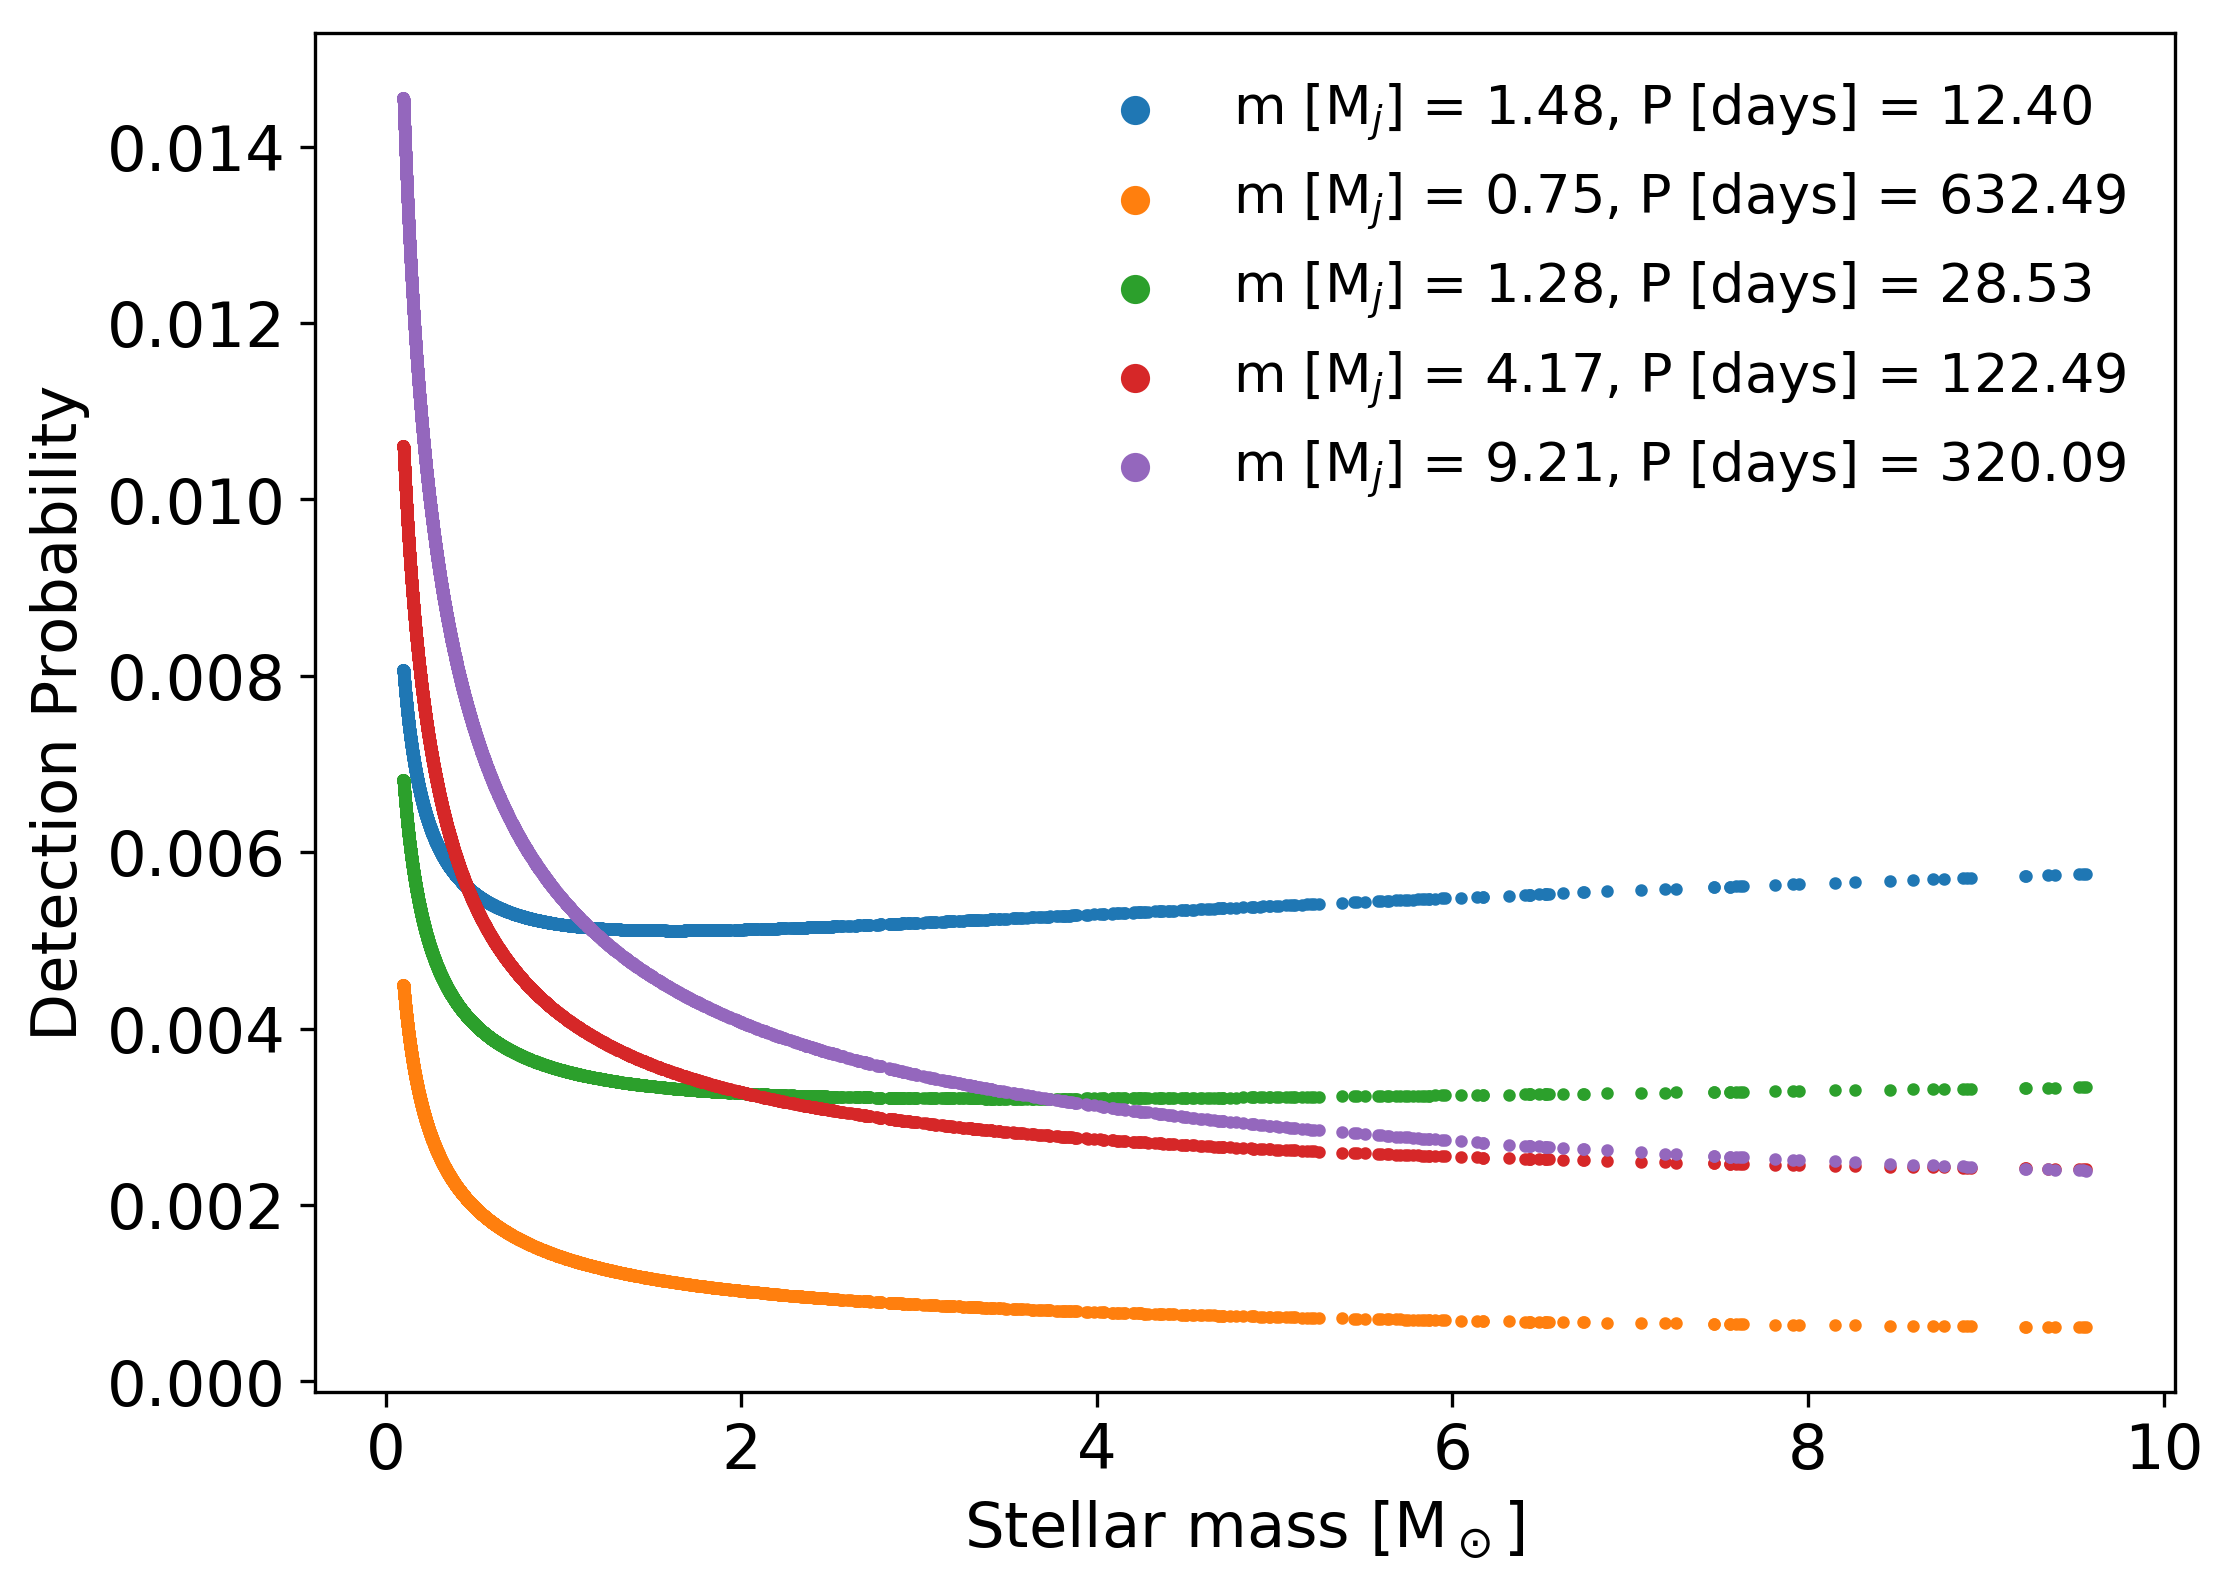
\includegraphics[width = 10cm, height = 7cm]{./Graficos/Capitulo_2/2_Exop_distributions/Monte-Carlo_KroupaNielsen.png} }}%
    \qquad
    \subfloat[]{{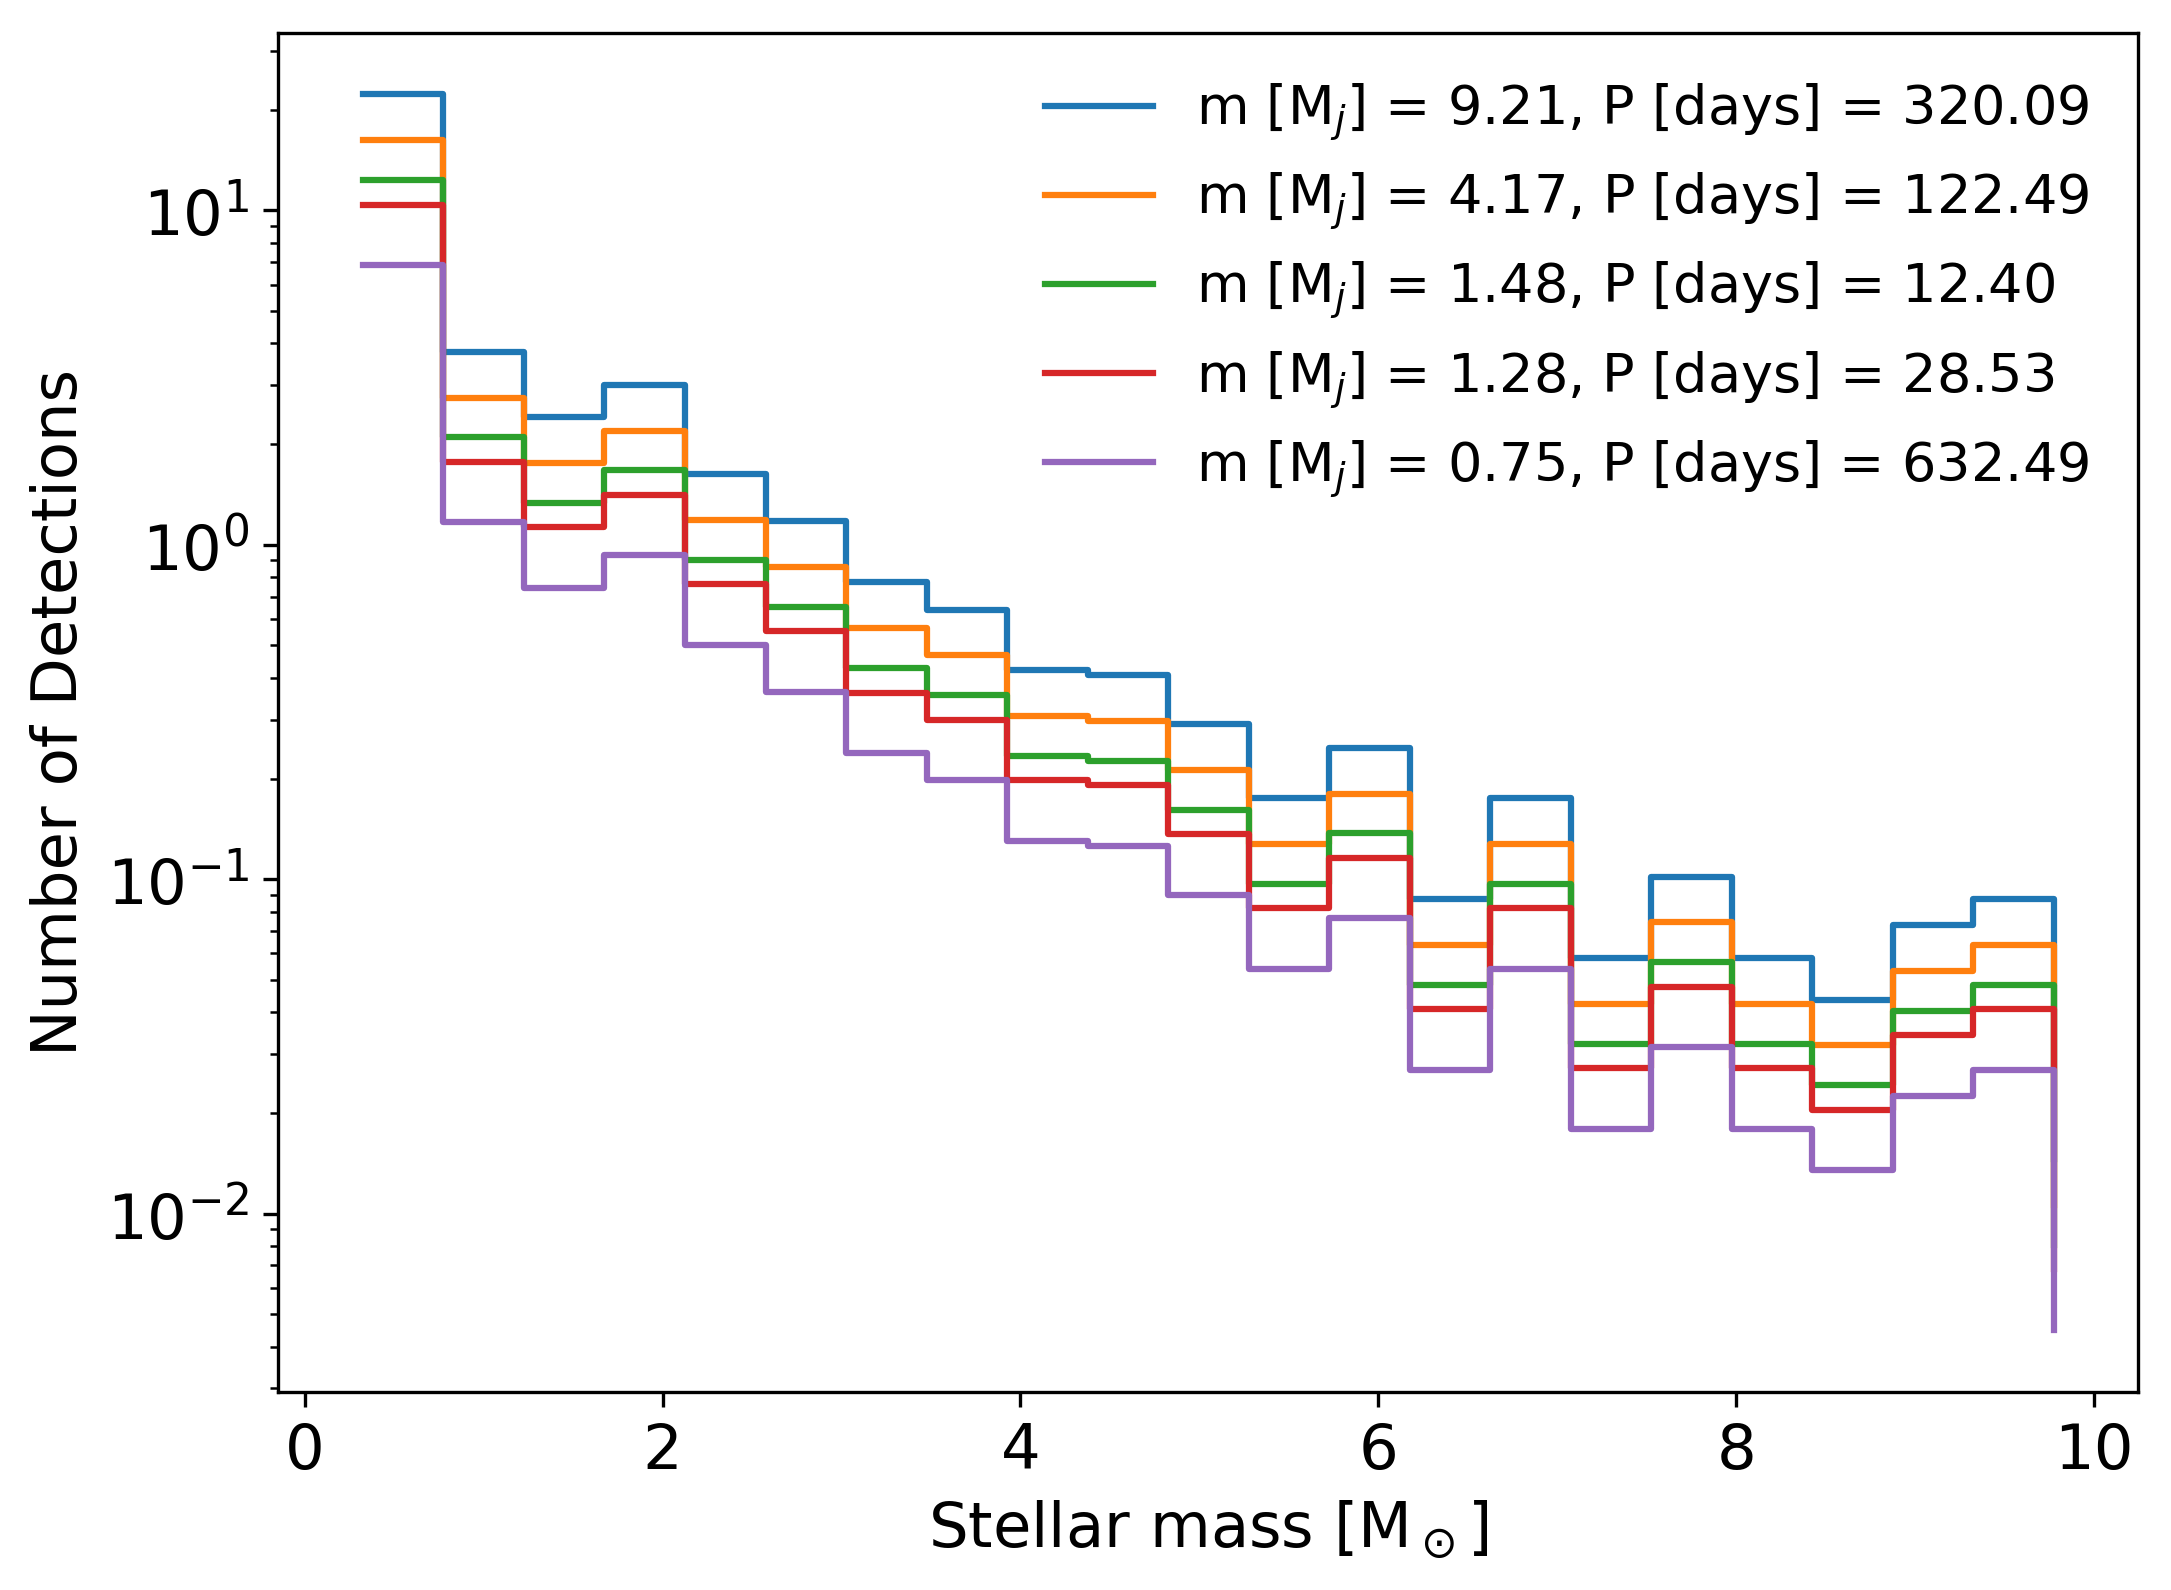
\includegraphics[width = 10cm, height = 7cm]{./Graficos/Capitulo_2/2_Exop_distributions/Monte-Carlo_KroupaNielsen_1.png} }}%
    \caption{\scriptsize{Detection probability and expected number of detections as a function of stellar mass. \textit{\textbf{(a)-panel}}: Detection probability of exoplanetary ringed systems as a function of stellar mass. Each curve corresponds to five-random-selected mass-period pairs used in \autoref{eq:FinalDetectProb}. In general, all curves follow the same trend, in which the best chance of detecting ring systems is around low-mass stars. \textit{\textbf{(b)-panel}}: Expected number of detections as a function of stellar mass. Each curve corresponds to the summed up values in each bin. The highest number of exoplanetary ringed systems are expected for stellar masses below $2 \textnormal{M}_\odot$.}}%
    \label{fig:MonteKroupaNielsen}%
\end{figure}

On the other hand, we evaluated directly \autoref{eq:FinalDetectProb} where instead of summing up each value inside a given bin, we integrate this function and use a weight to re-scale the values using the fact that as the stellar initial mass function follows a power law, it is possible to integrate each mass bin between boundaries $m_1$ and $m_2$ while leaving the total number of stars fixed i.e. $N = 10.000$, and finding the proportionality constant. This way is easier to compute the number of detections without recurring to a generation of large samples using the Monte-Carlo approach. To check this, we decided to test an exoplanet of $10\textnormal{Mj}$ and $5\textnormal{yr}$ period. First, using the Monte-Carlo process to generate the $10.000$ starts following the Kroupa distribution and evaluating \autoref{eq:FinalDetectProb} with fixed exoplanetary mass-period. After this, the detection probability was summed up in bins of $0.5M_\odot$ and the result is shown in \autoref{fig:MonteAnalytic_1}. However, for the second case, \autoref{eq:FinalDetectProb} was directly evaluated in a regular stellar mass array without any Monte-Carlo approach, and the detection probability was integrated fixing the total number of stars to re-scale each bin. The final result is shown in \autoref{fig:MonteAnalytic_1}. Both approaches lead to similar results, although in the case of the analytic form the slope is a bit steeper due to the fact that we are considering a fixed number of stars per bin derived from the continuity equation of the power law as explained before. If we reproduce the Monte-Carlo process several times we will eventually end up in this case. In brief, the analytic form approach will be used to study the dependence of this detection probability and the number of expected detections as a function of the fifth probability which was not introduced here and it is related to the lifetime of the planetary rings.\\

\begin{figure}[!ht]%
    \centering
    \subfloat{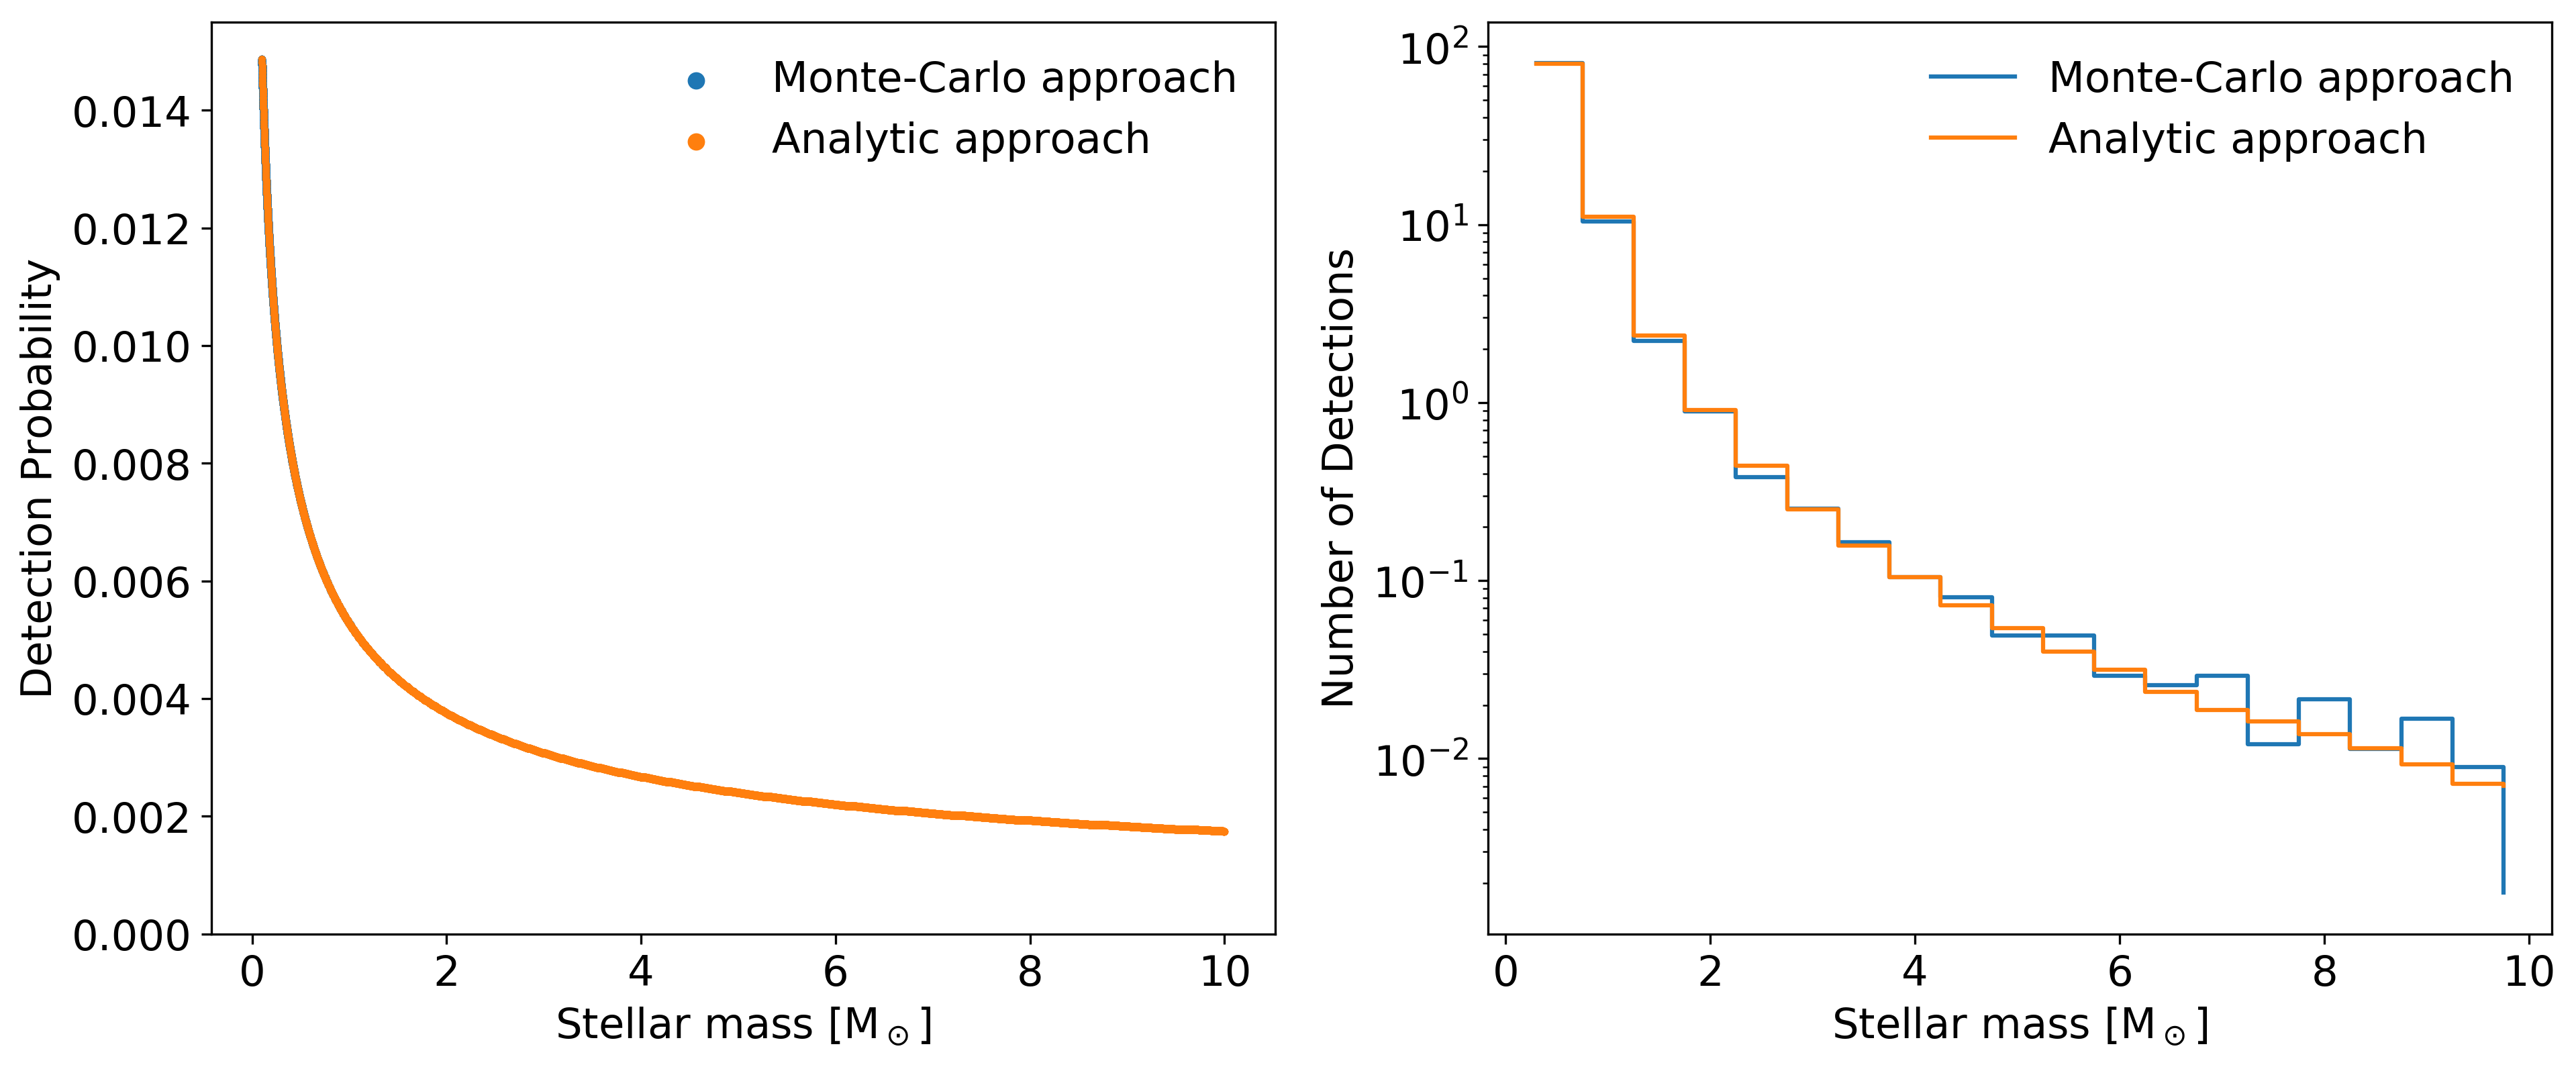
\includegraphics[width = 16cm, height = 6.5cm]{./Graficos/Capitulo_2/2_Exop_distributions/MC_Analytic.png} }%
    \caption{\scriptsize{Detection probability and expected number of detections as a function of stellar mass for an exoplanet of $10 \textnormal{Mj}$ mass and $5 \textnormal{yr}$ period. \textit{\textbf{left}}: Detection probability of an exoplanetary ringed system as a function of stellar mass. The blue and orange curves corresponds to one mass-period pair used in \autoref{eq:FinalDetectProb}. \textit{\textbf{right}}: Expected number of detections as a function of stellar mass. This is generated using the Monte-Carlo and analytic approaches.}}%
    \label{fig:MonteAnalytic_1}%
\end{figure}

% \begin{figure}[!ht]%
%     \centering
%     \subfloat[]{{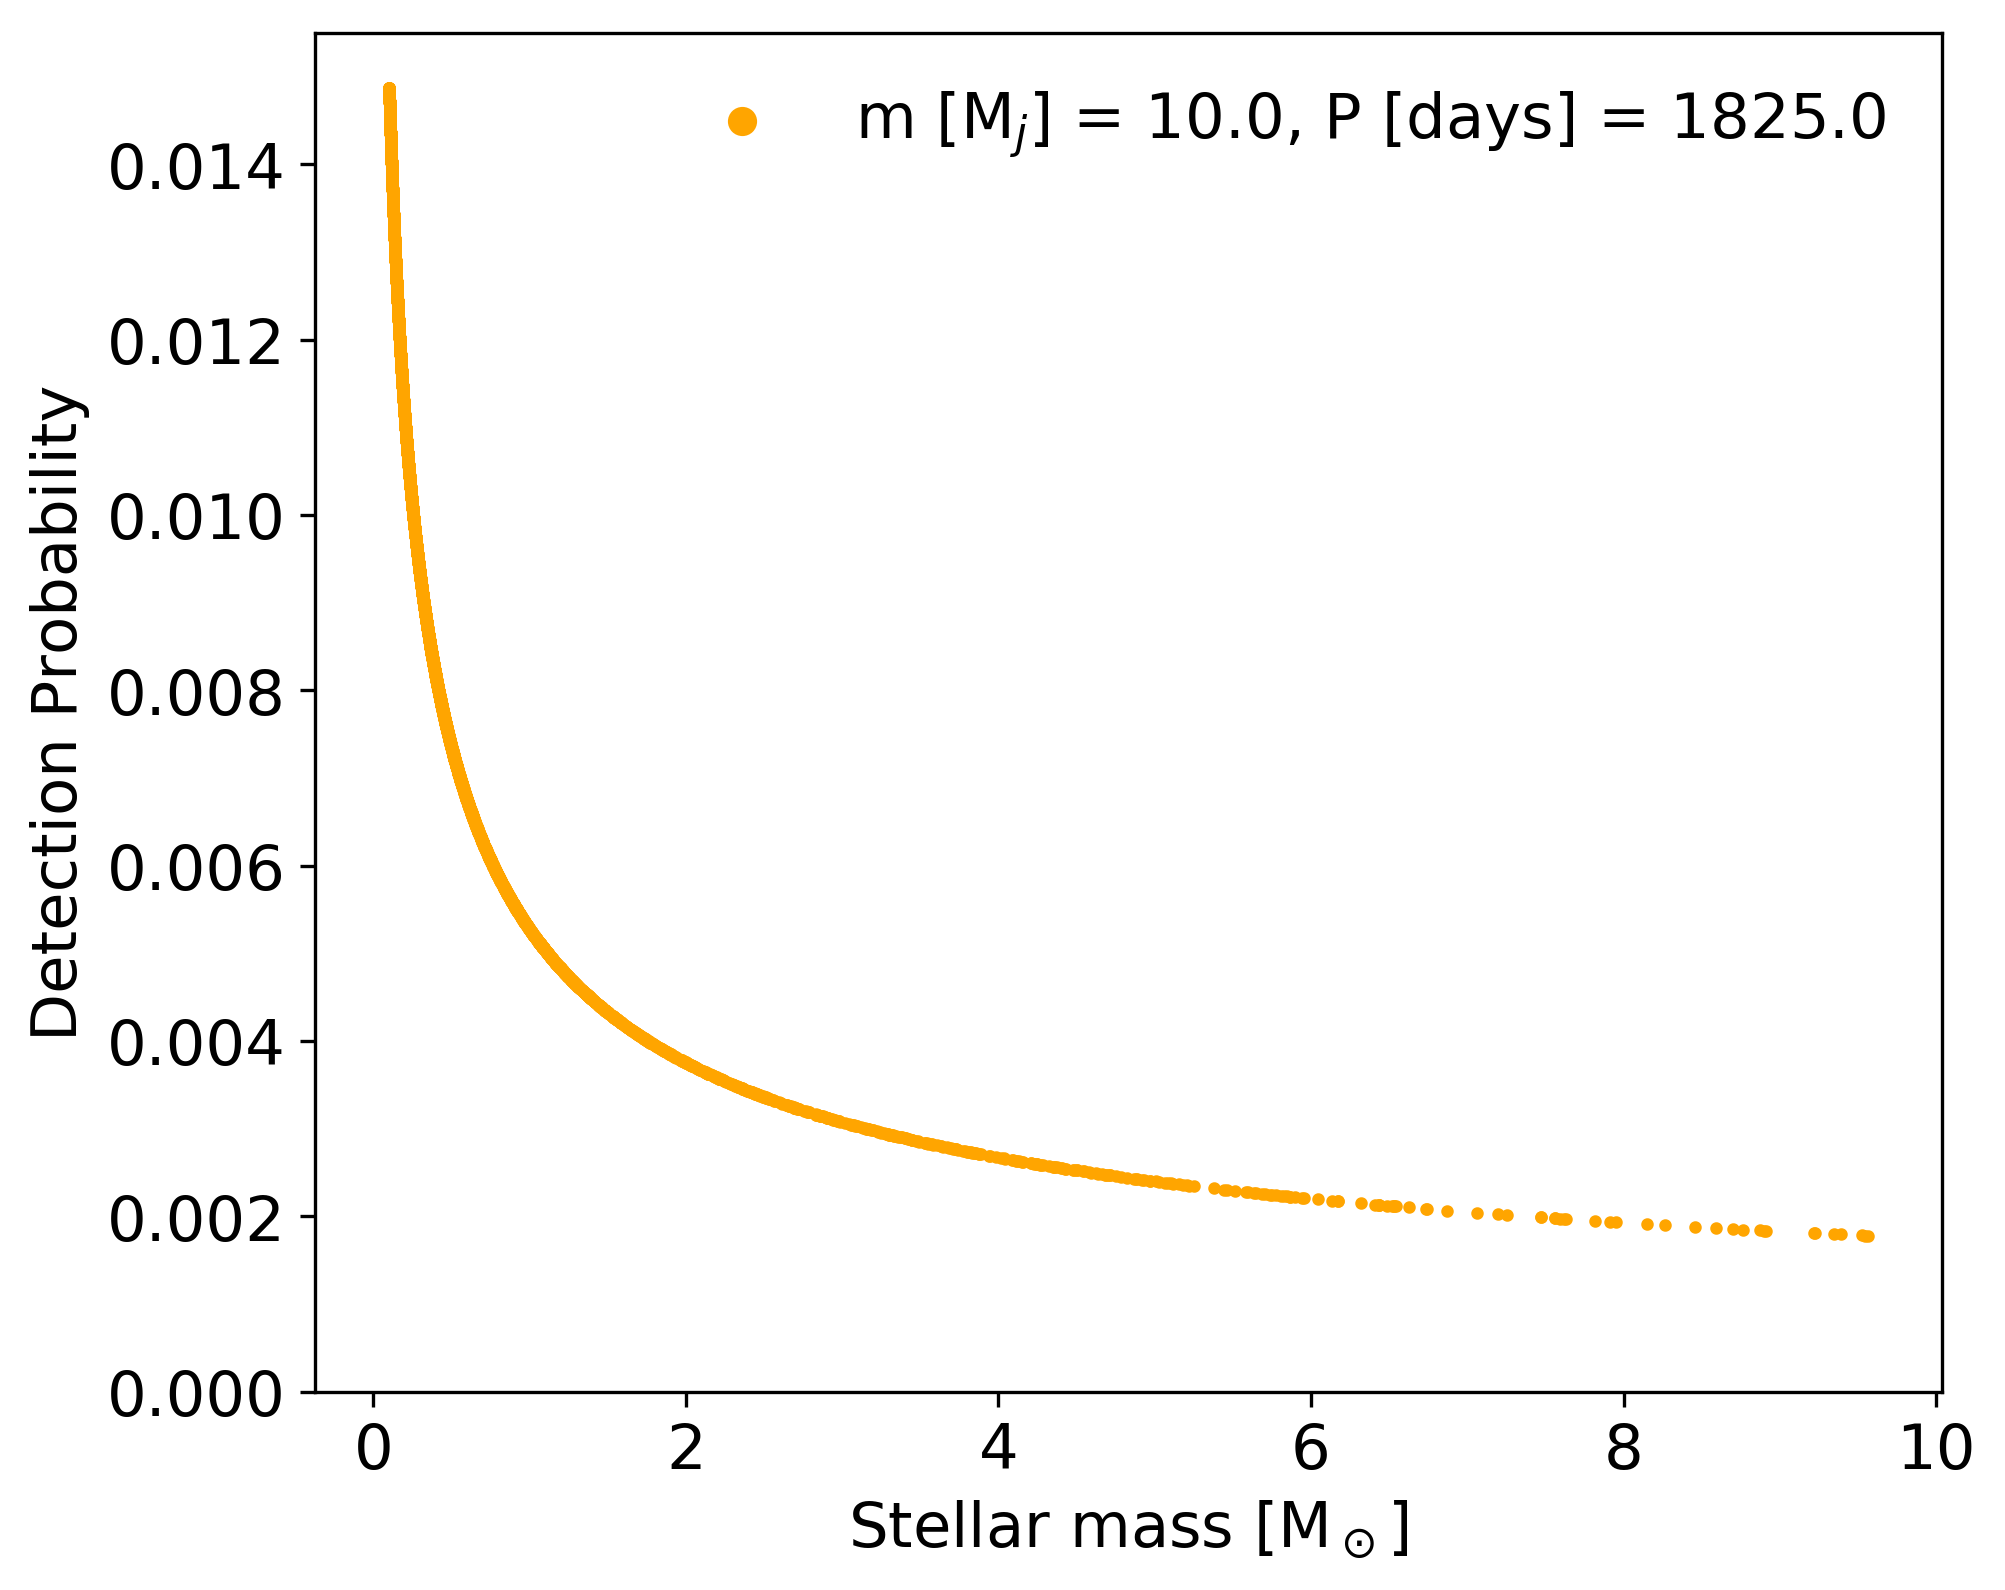
\includegraphics[width = 10cm, height = 7cm]{./Graficos/Capitulo_2/2_Exop_distributions/Monte-Carlo_KroupaNielsen_2.png} }}%
%     \qquad
%     \subfloat[]{{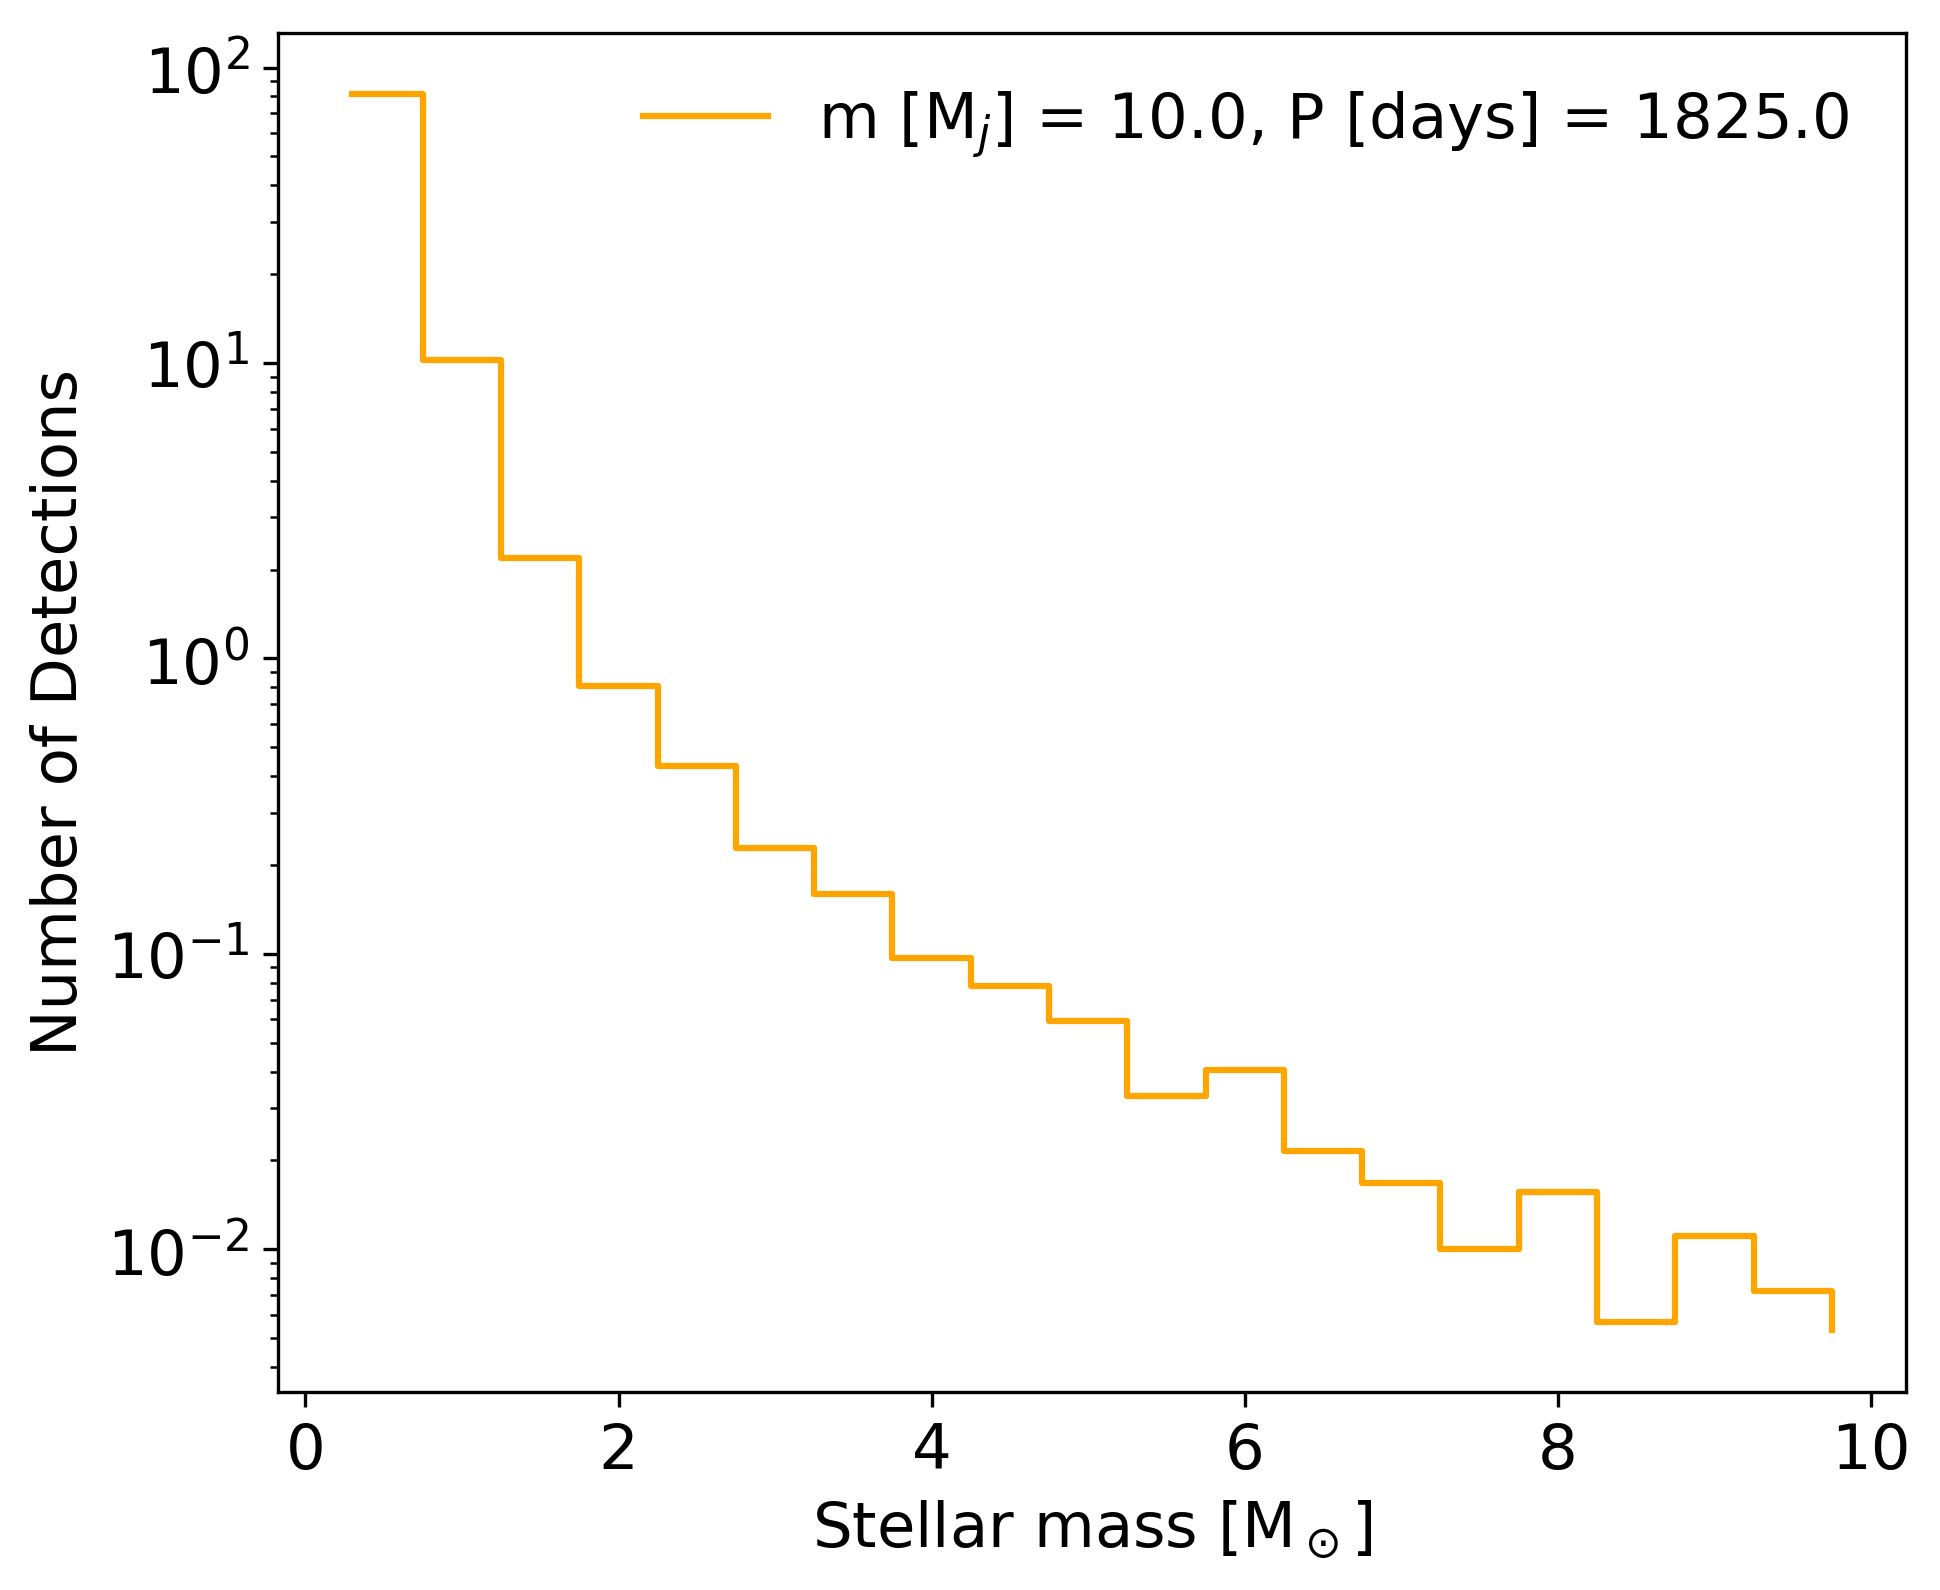
\includegraphics[width = 10cm, height = 7cm]{./Graficos/Capitulo_2/2_Exop_distributions/Monte-Carlo_KroupaNielsen_3.png} }}%
%     \caption{\scriptsize{Detection probability and expected number of detections as a function of stellar mass for an exoplanet of $10 \textnormal{Mj}$ mass and $5 \textnormal{yr}$ period. \textit{(a)-panel}: Detection probability of an exoplanetary ringed system as a function of stellar mass. The curve corresponds to one mass-period pair used in \autoref{eq:FinalDetectProb}. \textit{(b)-panel}: Expected number of detections as a function of stellar mass. This is generated using the Monte-Carlo approach and is shown to compare the analytic results obtained in \autoref{fig:MonteAnalytic_1}.}}%
%     \label{fig:MonteAnalytic_1}%
% \end{figure}
% 
% \begin{figure}[!ht]%
%     \centering
%     \subfloat[]{{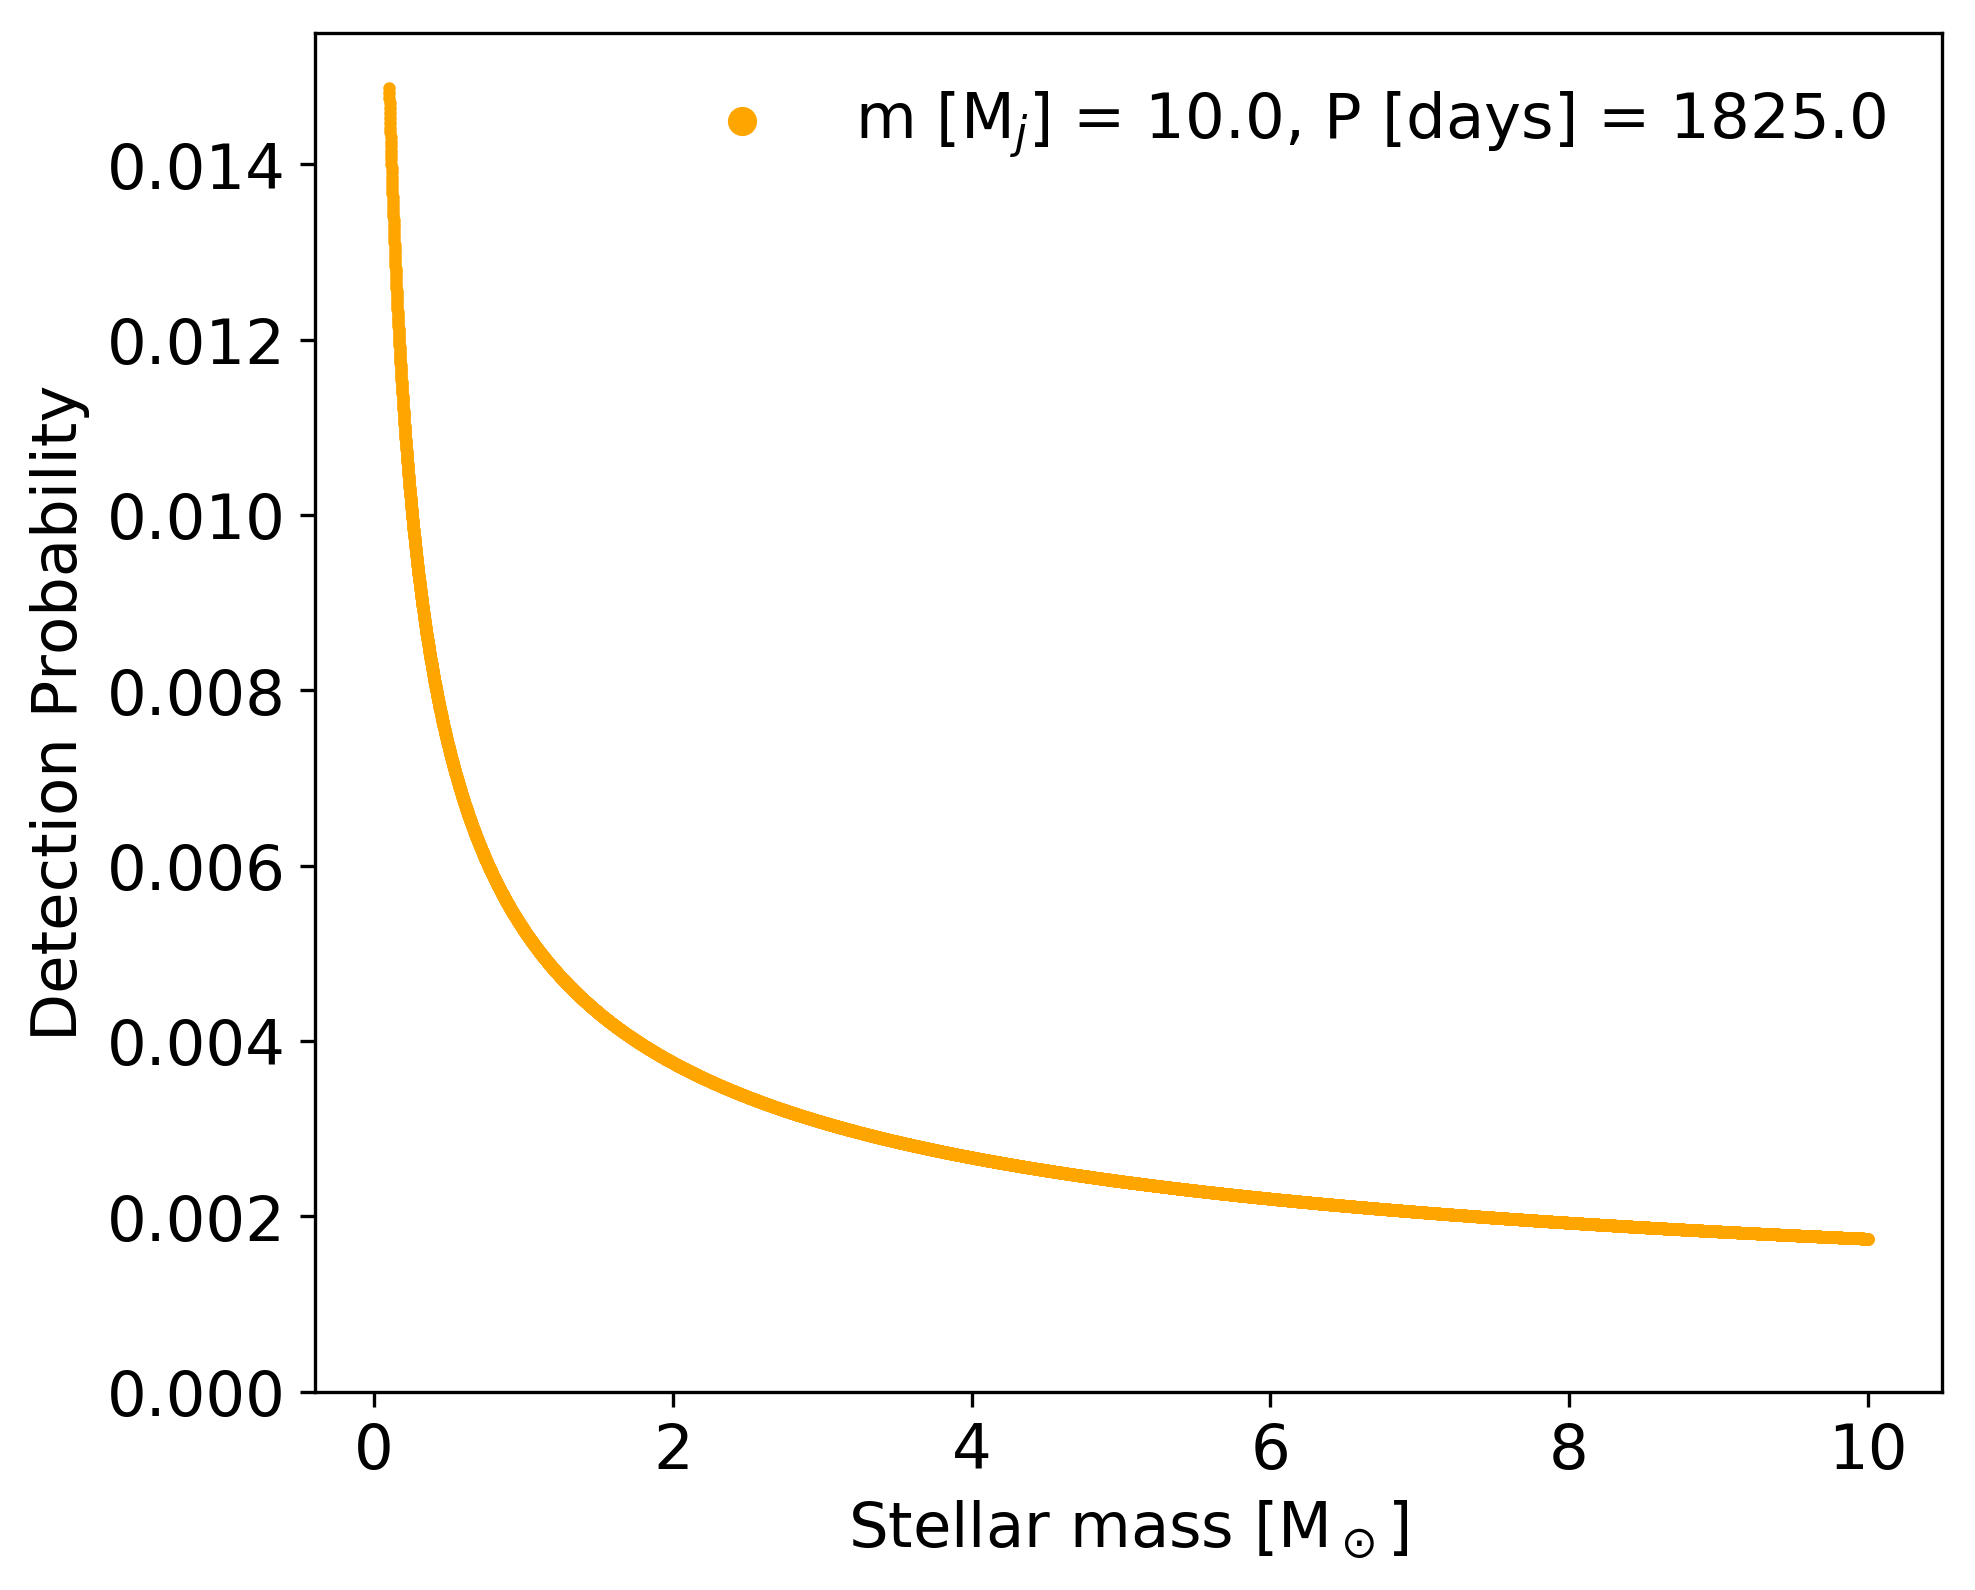
\includegraphics[width = 10cm, height = 7cm]{./Graficos/Capitulo_2/2_Exop_distributions/Analytic_Kroupa_Nielsen.png} }}%
%     \qquad
%     \subfloat[]{{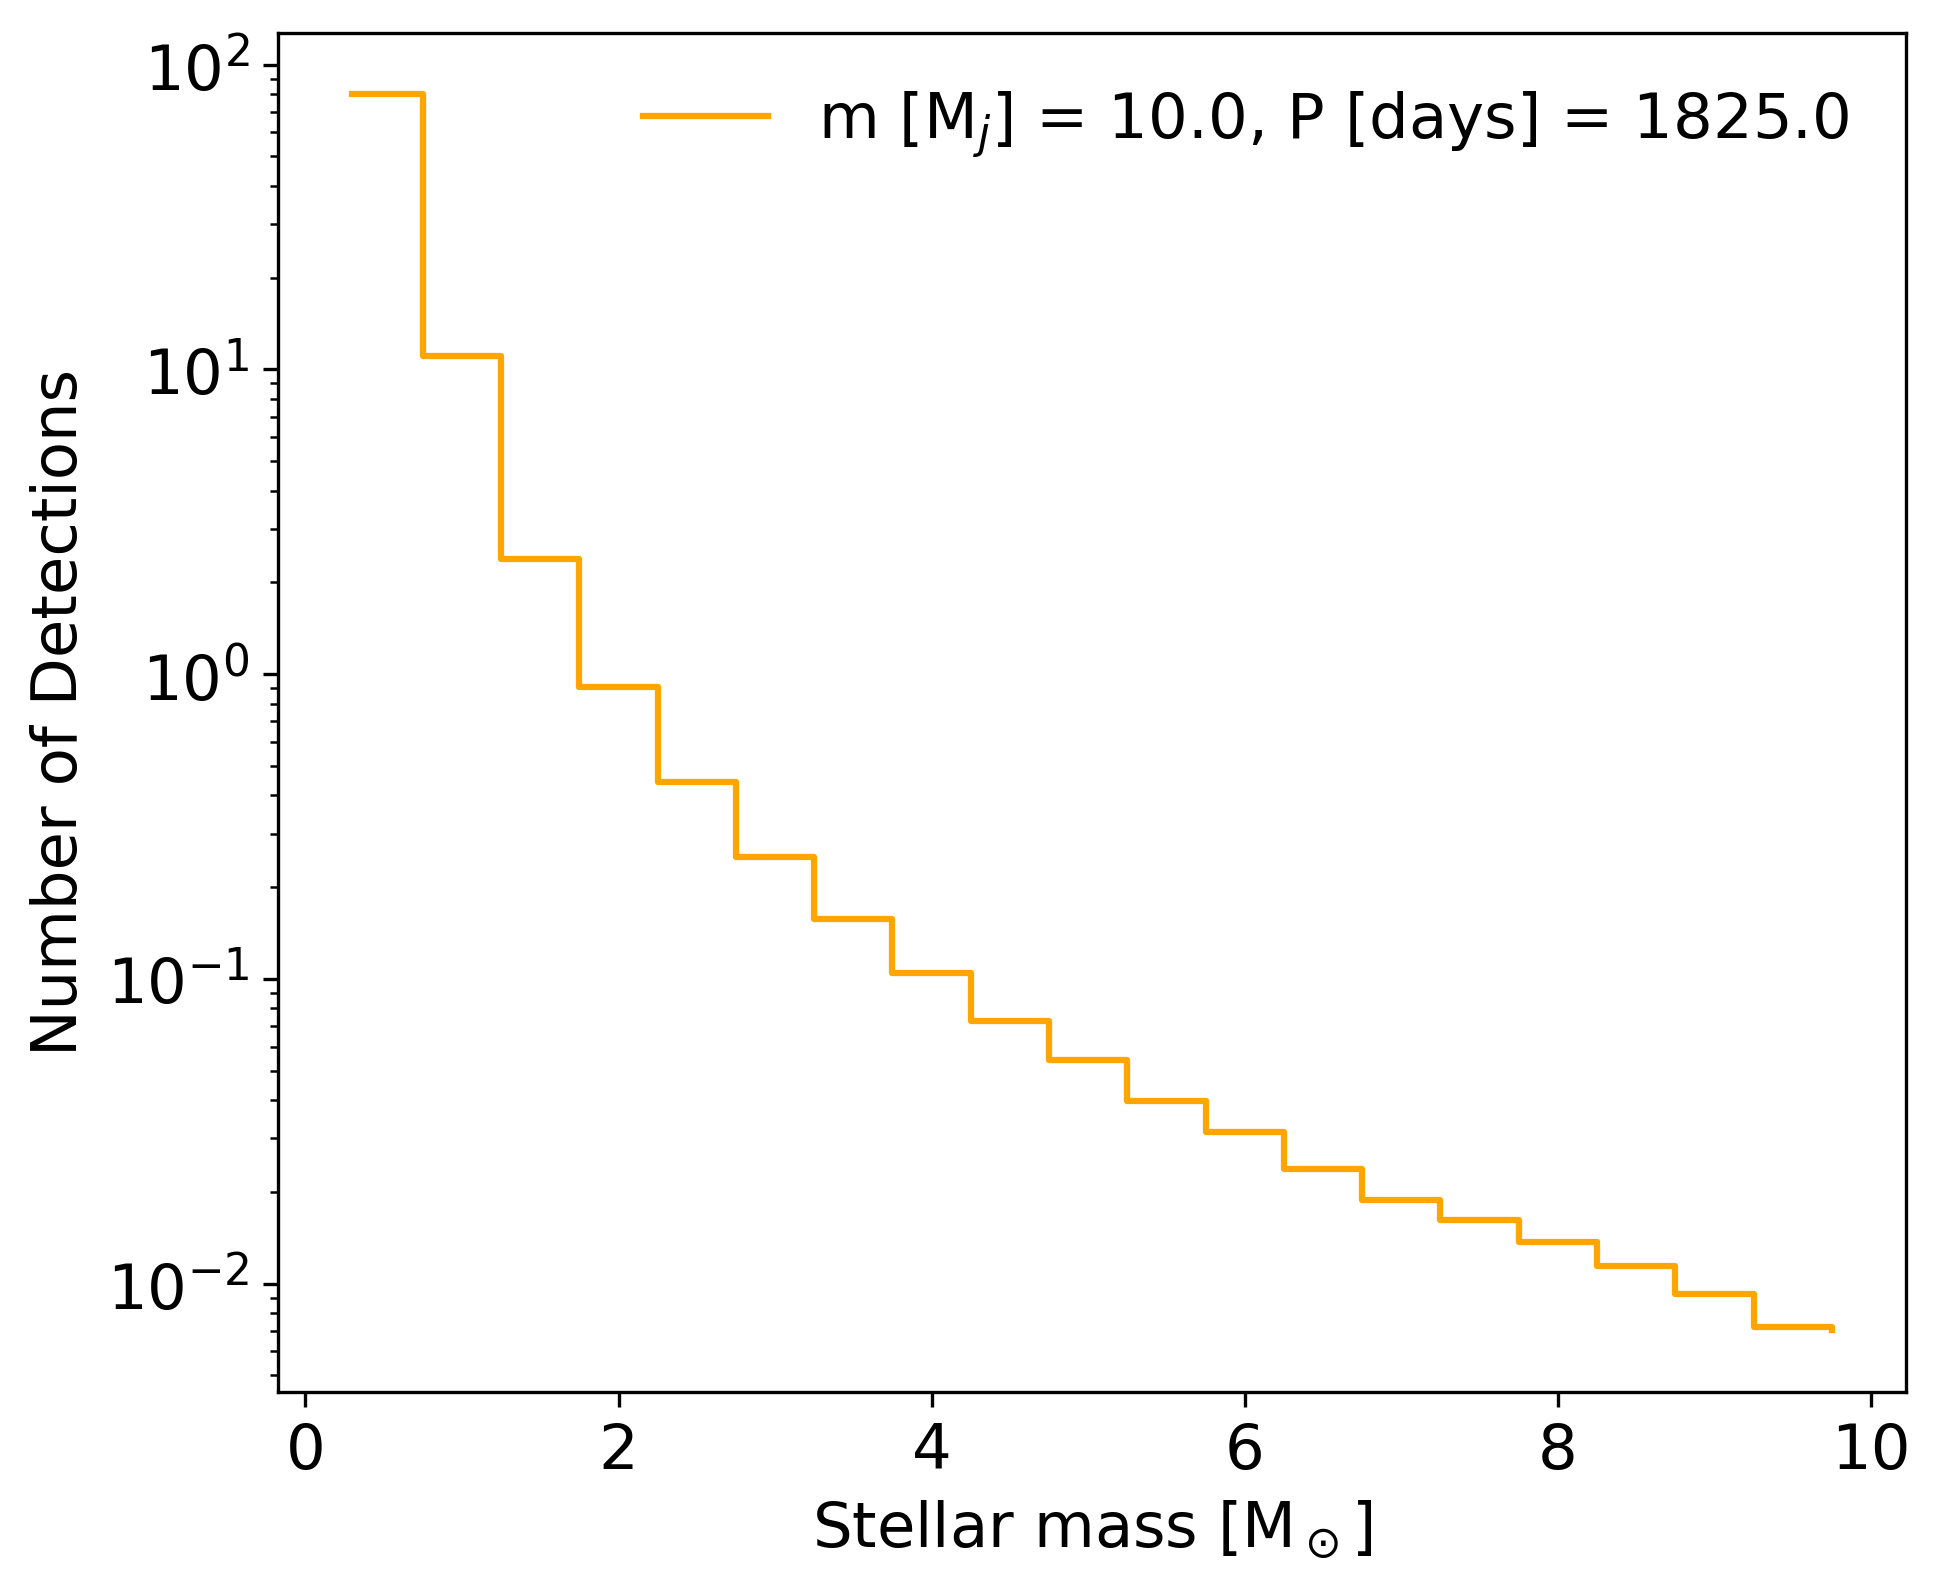
\includegraphics[width = 10cm, height = 7cm]{./Graficos/Capitulo_2/2_Exop_distributions/Analytic_Kroupa_Nielsen_1.png} }}%
%     \caption{\scriptsize{Detection probability and expected number of detections as a function of stellar mass for an exoplanet of $10 \textnormal{Mj}$ mass and $5 \textnormal{yr}$ period using an analytic approach. \textit{(a)-panel}: Detection probability of an exoplanetary ringed system as a function of stellar mass. The curve corresponds to one mass-period pair used in \autoref{eq:FinalDetectProb}. \textit{(b)-panel}: Expected number of detections as a function of stellar mass. This is generated using an analytic approach instead of the Monte-Carlo simulation shown in \autoref{fig:MonteAnalytic_1}.}}%
%     \label{fig:MonteAnalytic_1}%
% \end{figure}

Besides, tt was pointed out in \autoref{subsec:RingsSec} that there is no general consensus on the timescale in which planetary rings are formed or for how long they survive. However, based on evidence from our own solar system there is a range of possible values which will give a glimpse on this value. We decided to test how the detection probability and the number of detections change for different values. In \autoref{fig:Rings_Prob} each line was computed using the last method, avoiding the Monte-Carlo calculation for different rings' lifetime spanning from $1\times 10^5$yr to $1\times 10^7$yr because it was the most reliable range of values found in the literature. The case in which the fifth probability is not taken into account corresponds to an infinite timescale. It is clear that the younger the exoplanetary rings, the lower the probability of detecting them around the stellar system because as was shown in \autoref{eq:Prob_5} this probability is computed as a ratio between the rings' lifetime and the stellar age. Thus, the larger the timescale, the larger the probability, and so the detections. This is really important because depending on this value we can expect a different number of transits in a certain stellar mass range. However, it is worth noting that the highest probability is achieved towards the small stellar mass values.\\

\begin{figure}[!ht]
\centering
  \subfloat{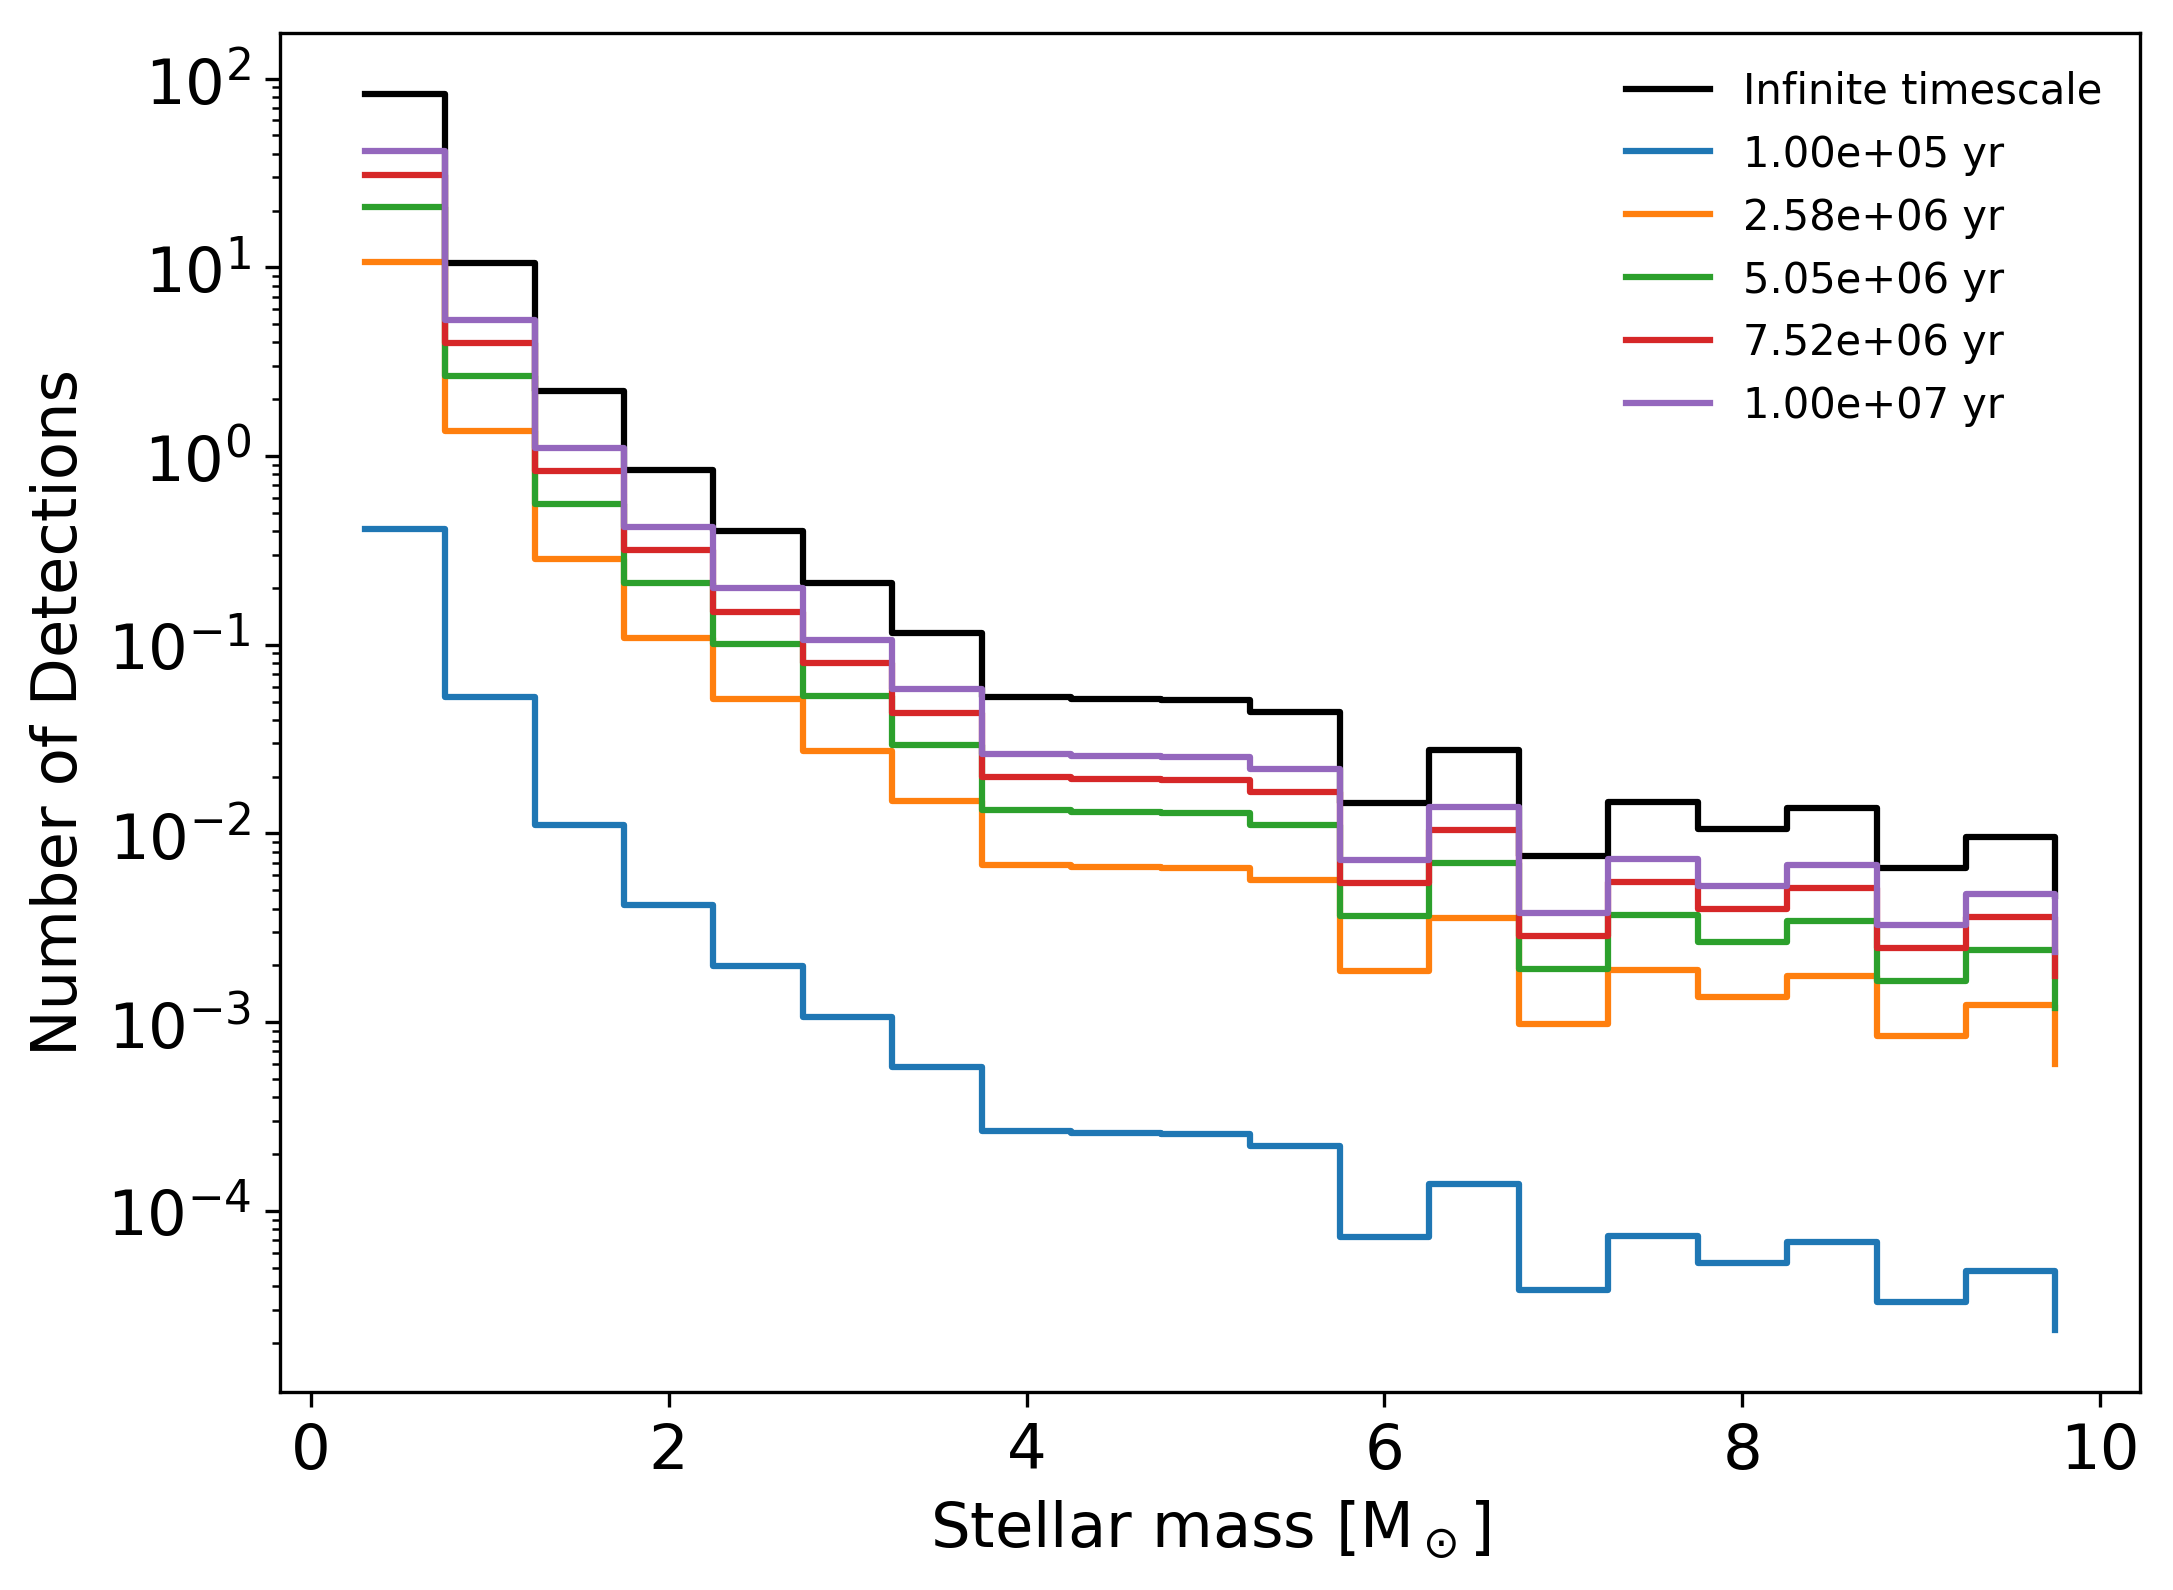
\includegraphics[width = 12cm, height = 9cm]{./Graficos/Capitulo_2/2_Exop_distributions/Analytic_rings_Kroupa_Nielsen.png}} 
\caption{\scriptsize{Expected number of detections as a function of stellar mass accounting for the rings' lifetime contribution. $0.0 \textnormal{yr}$ corresponds to a system where the rings are in place since the stellar and planet formation process until it is observed. Different times represent the lifespan of the exoplanetary rings. As the lifetime increases, also does the number of detections as the chance to observe an exoring in the system increases, converging to its maximum value if we assume the exorings to have an infinite lifetime.}}
\label{fig:Rings_Prob}
\end{figure}

In conclusion, we present different ways to calculate the expected number of detections. However, we decided to stick to the analytic form instead of using the Monte-Carlo process just for simplicity though both methods lead to the same results in overall. Also, there are different ways to generate the stellar masses using the Salpeter or Kroupa's initial mass functions. All the methods explained above are available in the Git-Hub repository \url{https://github.com/Jurgenvilla/Exoplanet-Rings-and-Gaia}. It is, however, worth noting that the main conclusion from this analysis relies on the fact that the number of planetary detections increases for the low-mass stars. Then, it is a good idea to focus on young stellar populations when looking for ring systems because they are mainly composed of proto-stars which are accreting gas and are still in the formation process. It is expected to test these assumptions and how reliable each probability involved in this process is with actual observations. 
%*****************************************
\chapter{\textbf{Gaia and SuperWASP sample data}} \label{ch: Data}
%*****************************************
\vspace{0.5cm} 
%============================================================================================================================================================

\section{Introduction}

The main goal of the project is to target young-star populations to enhance the probability of observing exoplanetary rings transiting in front of their parent star as a result of the probabilistic analysis addressed in \autoref{ch: Model}. Therefore, we mainly focused our study in the well-known OB association ScoCen which is traditionally sub-divided into three different regions: \textit{Lower Centaurus Crux} (LCC), \textit{Upper Centaurus Lupus} (UCL), and \textit{Upper Scorpius} (US). The \textit{Gaia}-DR1 and-DR2 data were used to select the final sample of stars satisfying conditions on the distance, parallaxes and proper motions based on previous research (\cauthor{2018MNRAS.tmp..210W} \citeyear{2018MNRAS.tmp..210W}; \cauthor{2016MNRAS.461..794P} \citeyear{2016MNRAS.461..794P}; \cauthor{1989A&A...216...44D} \citeyear{1989A&A...216...44D}). However, also a selection based on stellar evolution tracks and isochrones using the \textit{MESA}-code provided through the \textit{MIST}-package (\cauthor{2016ApJS..222....8D} \citeyear{2016ApJS..222....8D}; \cauthor{2016ApJ...823..102C} \citeyear{2016ApJ...823..102C}) was performed to guarantee that the final sample consists of stars between $5$Myr to $60$Myr. This information is needed in order to obtain the $RA$ and $DEC$ coordinates of the objects of interest and retrieve the available light curves using the \textit{SuperWASP}-database (\cauthor{2006PASP..118.1407P} \citeyear{2006PASP..118.1407P}; \cauthor{2010A&A...520L..10B} \citeyear{2010A&A...520L..10B}). The main results from the \textit{Gaia}-and \textit{SuperWASP}-queries are presented in more detail in the next sections, including the light-curves preliminary results which are addressed extensively in \autoref{ch: Results} .   
%============================================================================================================================================================

% \section{ScoCen OB Association}
%============================================================================================================================================================

\section{Gaia Samples}\label{sec:GaiaSamples}

The \textit{Gaia}-DR1 and-DR2 data was used to select stars which belong to the ScoCen OB association. The queries were carried out using the ADQL-query interface provided by the ESA (\url{https://gea.esac.esa.int/archive/}) and shown in \autoref{ch:Appendix} for each of the three regions conforming ScoCen i.e. LCC, UCL, and US. The approach was tested in \textit{Gaia}-DR1, but later on was extended to the new data provided by the DR2 to increase the sample of stars belonging to ScoCen, and also to increase the chance of matching a star with a light curve in the \textit{SuperWASP}-database. This will be addressed at the end. The most relevant parameters retrieved for each object are the RA and DEC coordinates, galactic longitude (l) and latitude (b), parallax, the magnitude in the G-band, color index G-Ks, and the proper motion in RA and DEC.\\    

First of all, a sample based on previous physical parameters and values obtained for this association is needed in order to constrain the sample and avoid pollution from stars which may not be part of it. Following \cauthor{2018MNRAS.tmp..210W} (\citeyear{2018MNRAS.tmp..210W}), the spatial distribution of the three regions were selected using the galactic coordinates cut reported by \cauthor{2012yCat..74163108R} (\citeyear{2012yCat..74163108R}) and \cauthor{1999AJ....117..354D} (\citeyear{1999AJ....117..354D}) as shown in \autoref{tab:ScoCen_SpatialDist}. Also in distance, using a parallax range from $6$mas to $12$mas which leads to a distance range of $\sim 83-167$pc. We decided to include a wide range in distance because ScoCen is known to lie between $\sim 100-150$pc \cauthor{2018MNRAS.tmp..210W} (\citeyear{2018MNRAS.tmp..210W}), so we can include a larger sample and rule out any outliers based on the dynamics of the cluster. The spatial distribution of our sample is shown in \autoref{fig:Projection_ScoCen}. The blue, orange, and red dots represent LCC, UCL, and US respectively. It is clear that the ScoCen association covers a wide range in galactic longitude (l) $\sim 90$-deg, and $\sim 45$-deg in galactic latitude (b). Initially each sub-region contains LCC $= 2310$, UCL $= 1759$, and US $= 1584$ stars respectively. However, as it is mentioned in \cauthor{2016MNRAS.461..794P} (\citeyear{2016MNRAS.461..794P}), each region has a characteristic range for the proper motions given by the dynamics of each individual subgroup and the whole interaction. According to their work, the three subgroups have a value of $\mu_\alpha < 10~\textnormal{mas}~\textnormal{yr}^{-1}$ and $\mu_\delta < 30~\textnormal{mas}~\textnormal{yr}^{-1}$, while for LCC, UCL, and US values of $15~\textnormal{mas}~\textnormal{yr}^{-1} < \mu < 55~\textnormal{mas}~\textnormal{yr}^{-1}$, $12~\textnormal{mas}~\textnormal{yr}^{-1} < \mu < 55~\textnormal{mas}~\textnormal{yr}^{-1}$, and $\mu < 47~\textnormal{mas}~\textnormal{yr}^{-1}$, respectively, are reported. This is better seen in \autoref{fig:Hist_ScoCen_Mamajek} where the histogram for the whole sample of stars selected in distance range are shown in colors, and each vertical dashed-line shows the above mentioned cuts for each subgroup. In the end, after this analysis, the query was performed taking into account the dynamical constraints of the cluster (see \autoref{ch:Appendix}) to provide a clean sample.\\  

\begin{table}[]
\centering
\caption{\scriptsize{ScoCen subgroups galactic coordinates selection box.}}
\label{tab:ScoCen_SpatialDist}
\begin{tabular}{lcccc}
\hline
Sub-group             & l$_{-}$ {[}deg{]} & l$_{+}$ {[}deg{]} & b$_{-}$ {[}deg{]} & b$_{+}$ {[}deg{]} \\ \hline \hline
Lower Centaurus Crux  & 285               & 313               & -10               & 16                \\
Upper Centaurus Lupus & 313               & 337               & 5                 & 31                \\
Upper Scorpius        & 337               & 360               & 7                 & 32                \\ \hline \hline
\end{tabular}
\end{table}

\begin{figure}[!ht]%
    \centering
    \subfloat{{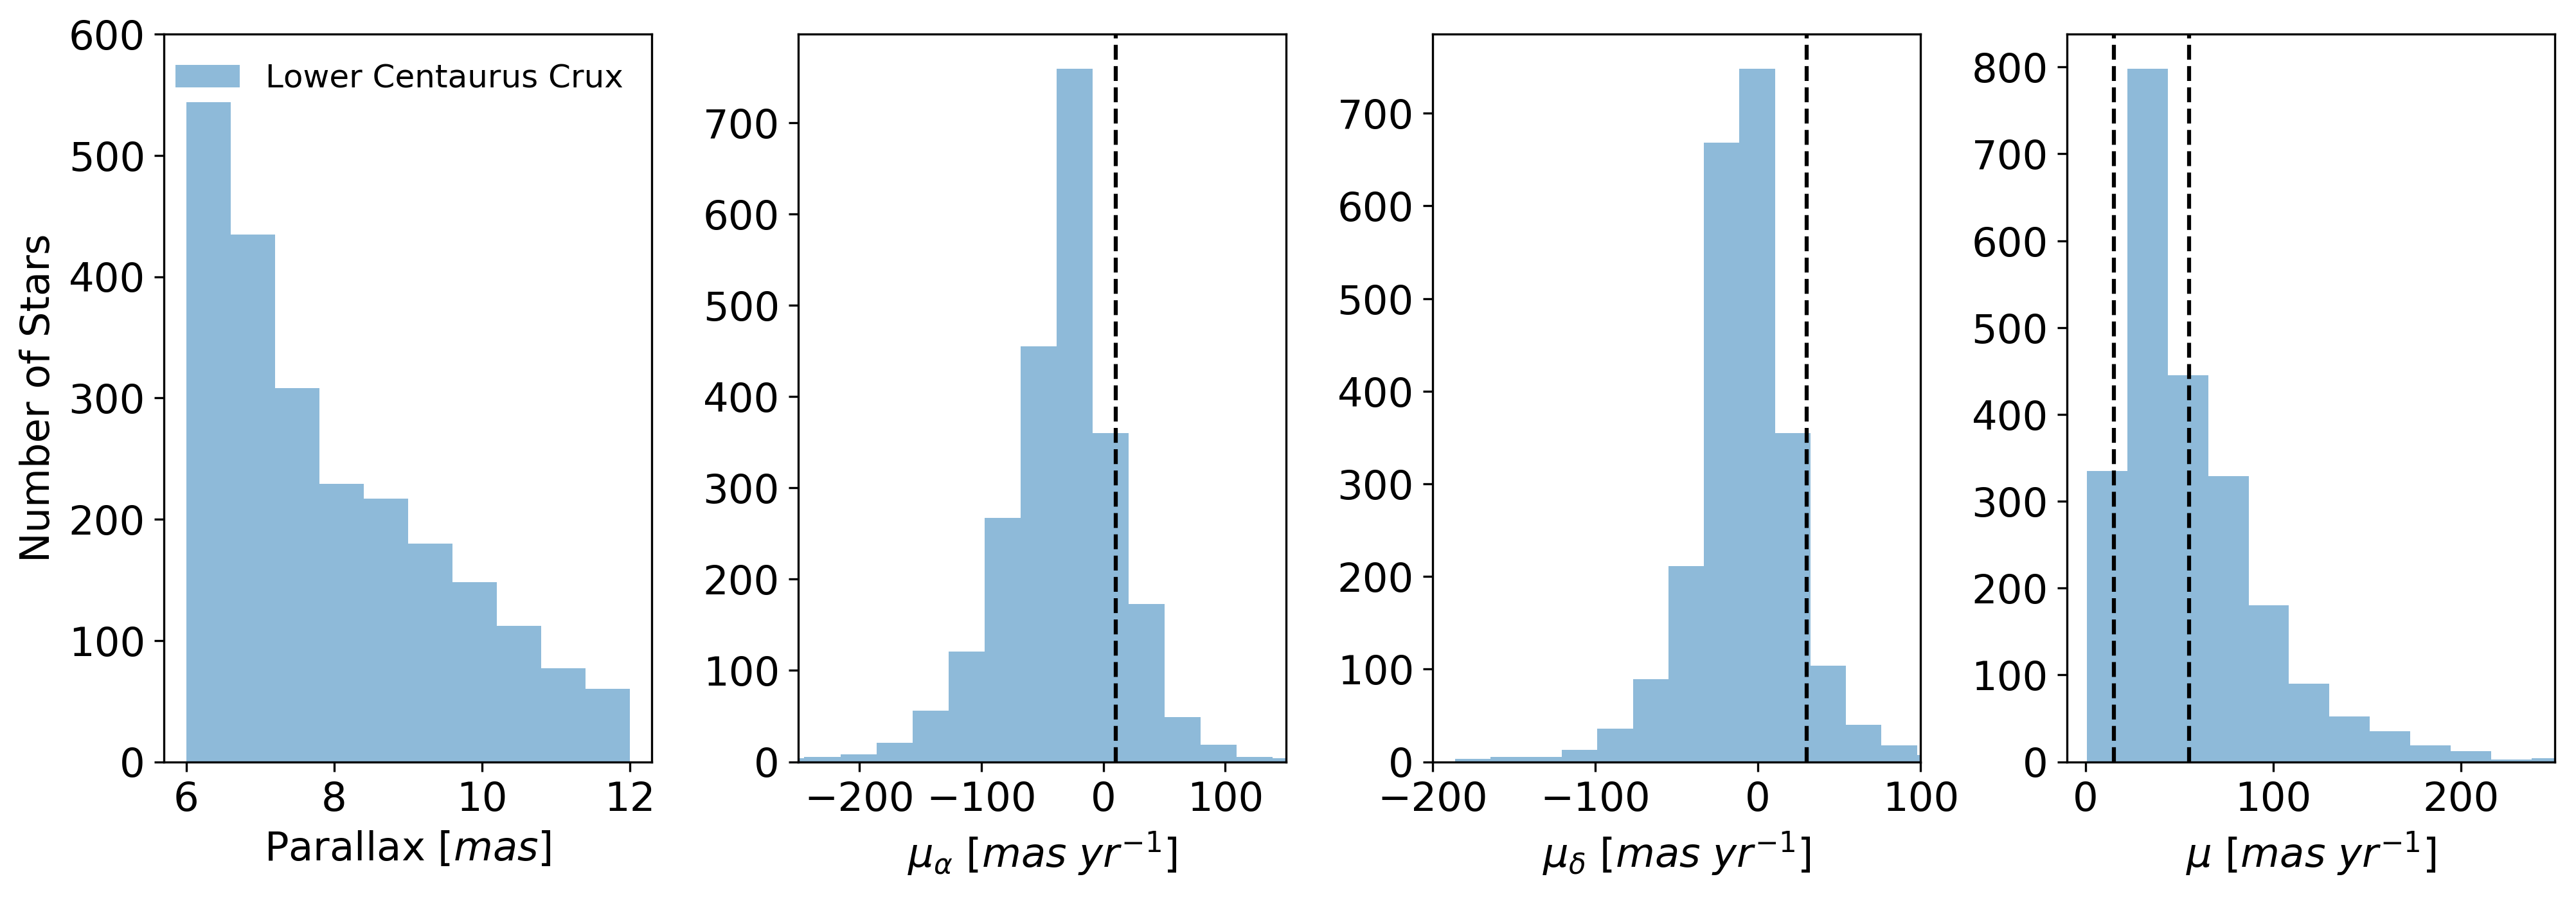
\includegraphics[width = 16cm, height = 5.5cm]{./Graficos/Capitulo_3/5_Sco-Cen/Hist_Extintion_1.png} }}%
    \qquad
    \subfloat{{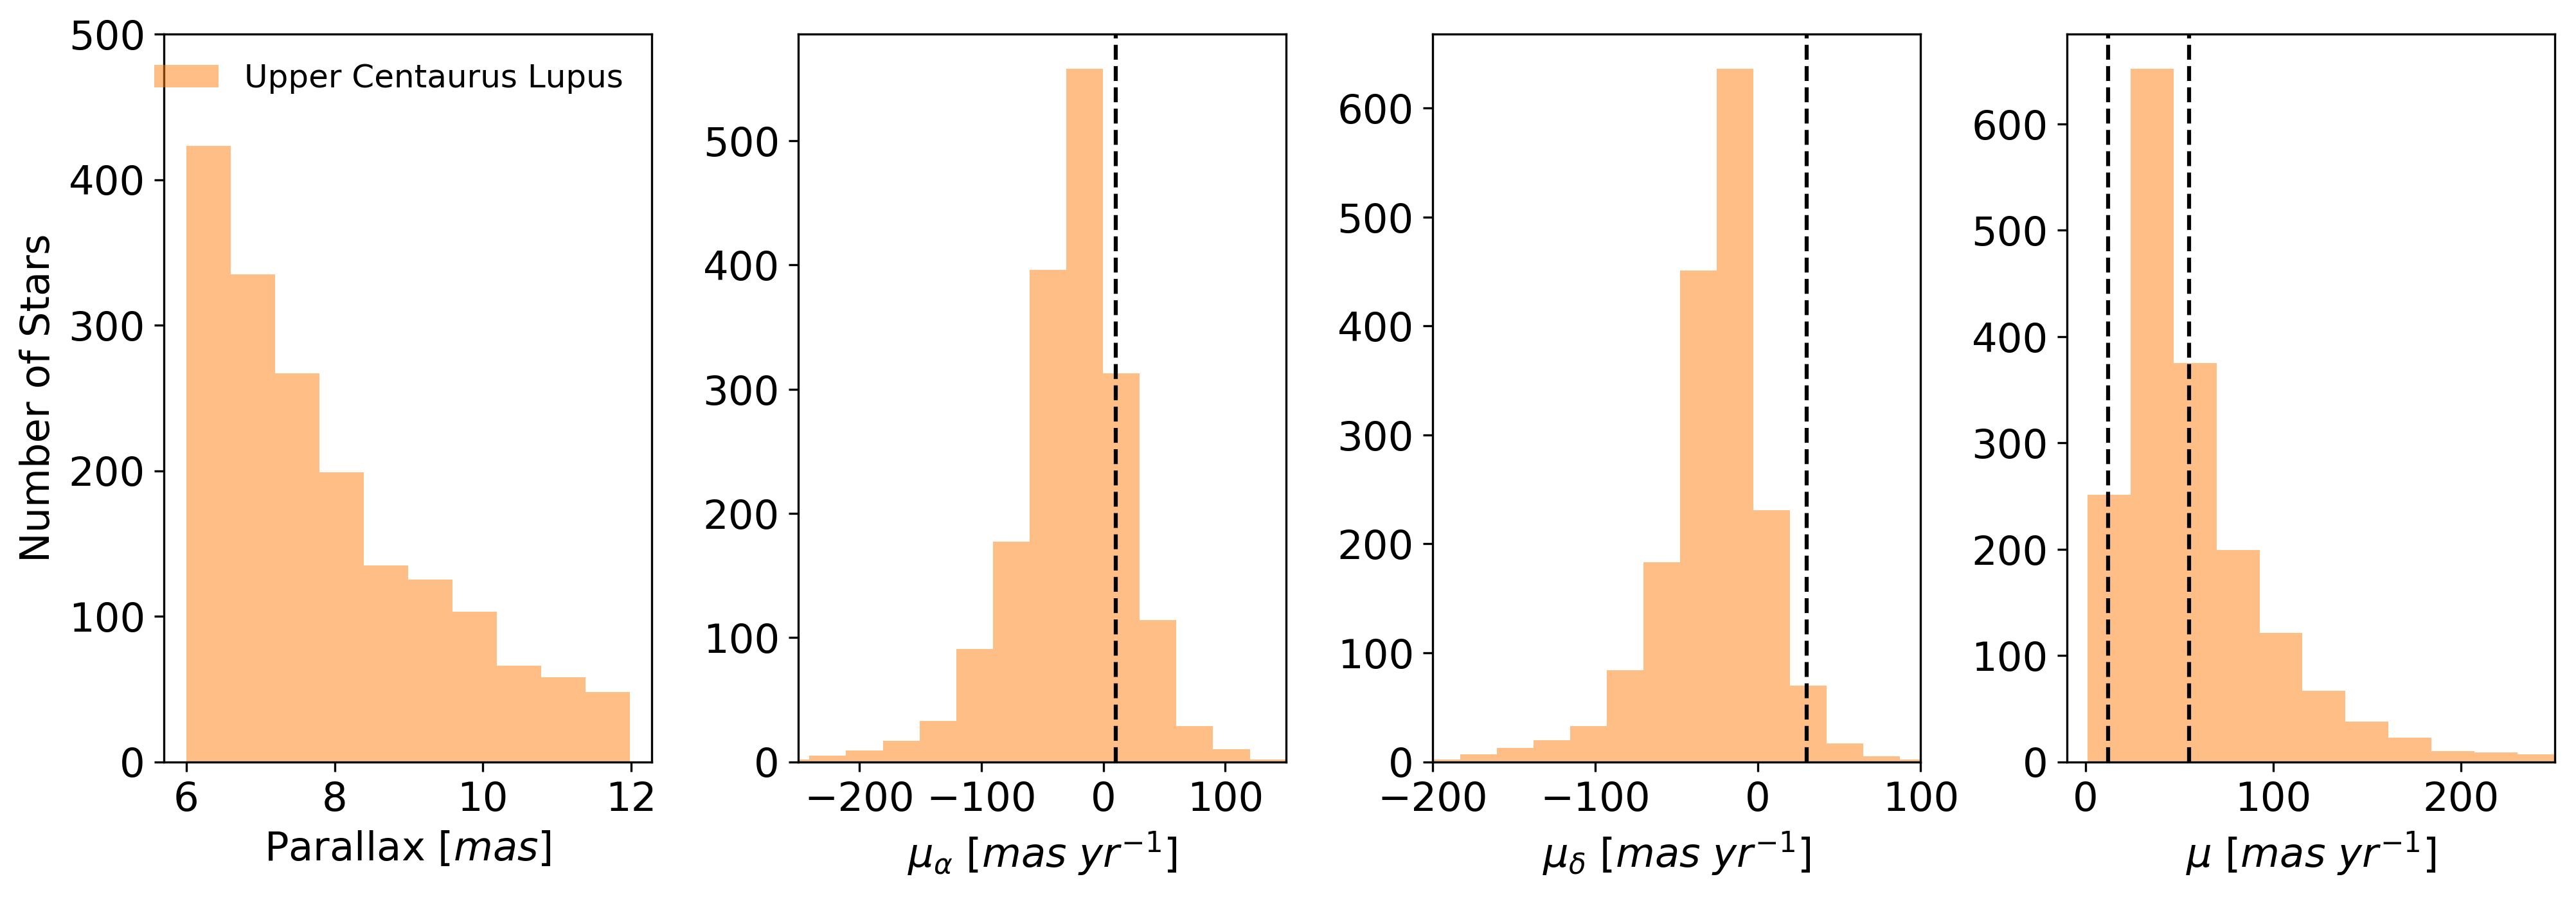
\includegraphics[width = 16cm, height = 5.5cm]{./Graficos/Capitulo_3/5_Sco-Cen/Hist_Extintion_2.png} }}%
    \qquad
    \subfloat{{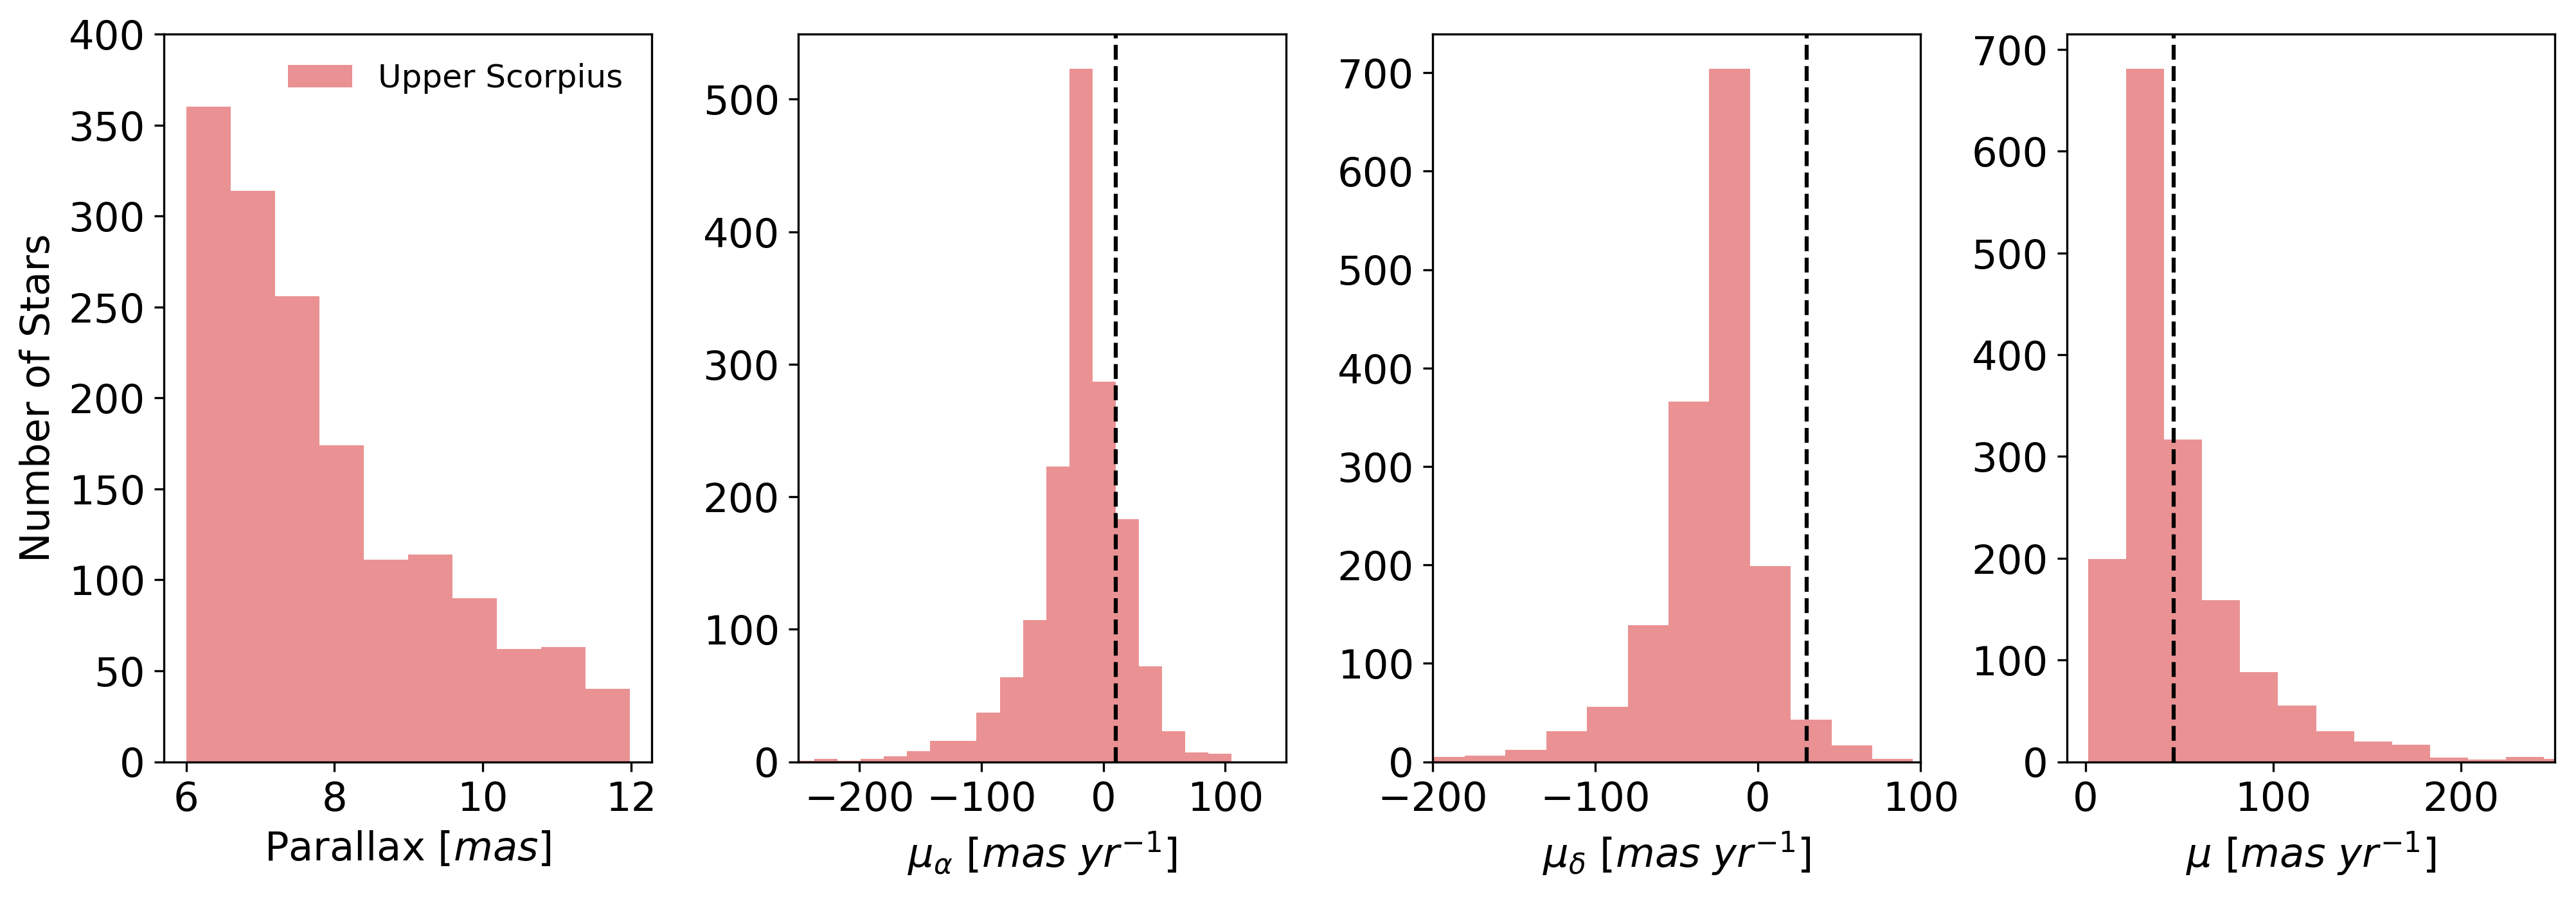
\includegraphics[width = 16cm, height = 5.5cm]{./Graficos/Capitulo_3/5_Sco-Cen/Hist_Extintion_3.png} }}%
    \caption{\scriptsize{Number of stars in LCC (blue), UCL (orange) and US (red), as a function of, from left to right, parallax, proper motion in right ascension, proper motion in declination and total proper motion. The parallax was set to satisfy ScoCen's distance range reported in literature. In the case of proper motion, cuts based on \cauthor{2018MNRAS.tmp..210W} (\citeyear{2018MNRAS.tmp..210W}) were applied, and are shown as black-dashed vertical lines.}}%
    \label{fig:Hist_ScoCen_Mamajek}%
\end{figure}  

\begin{figure}[!ht]
\centering
  \subfloat{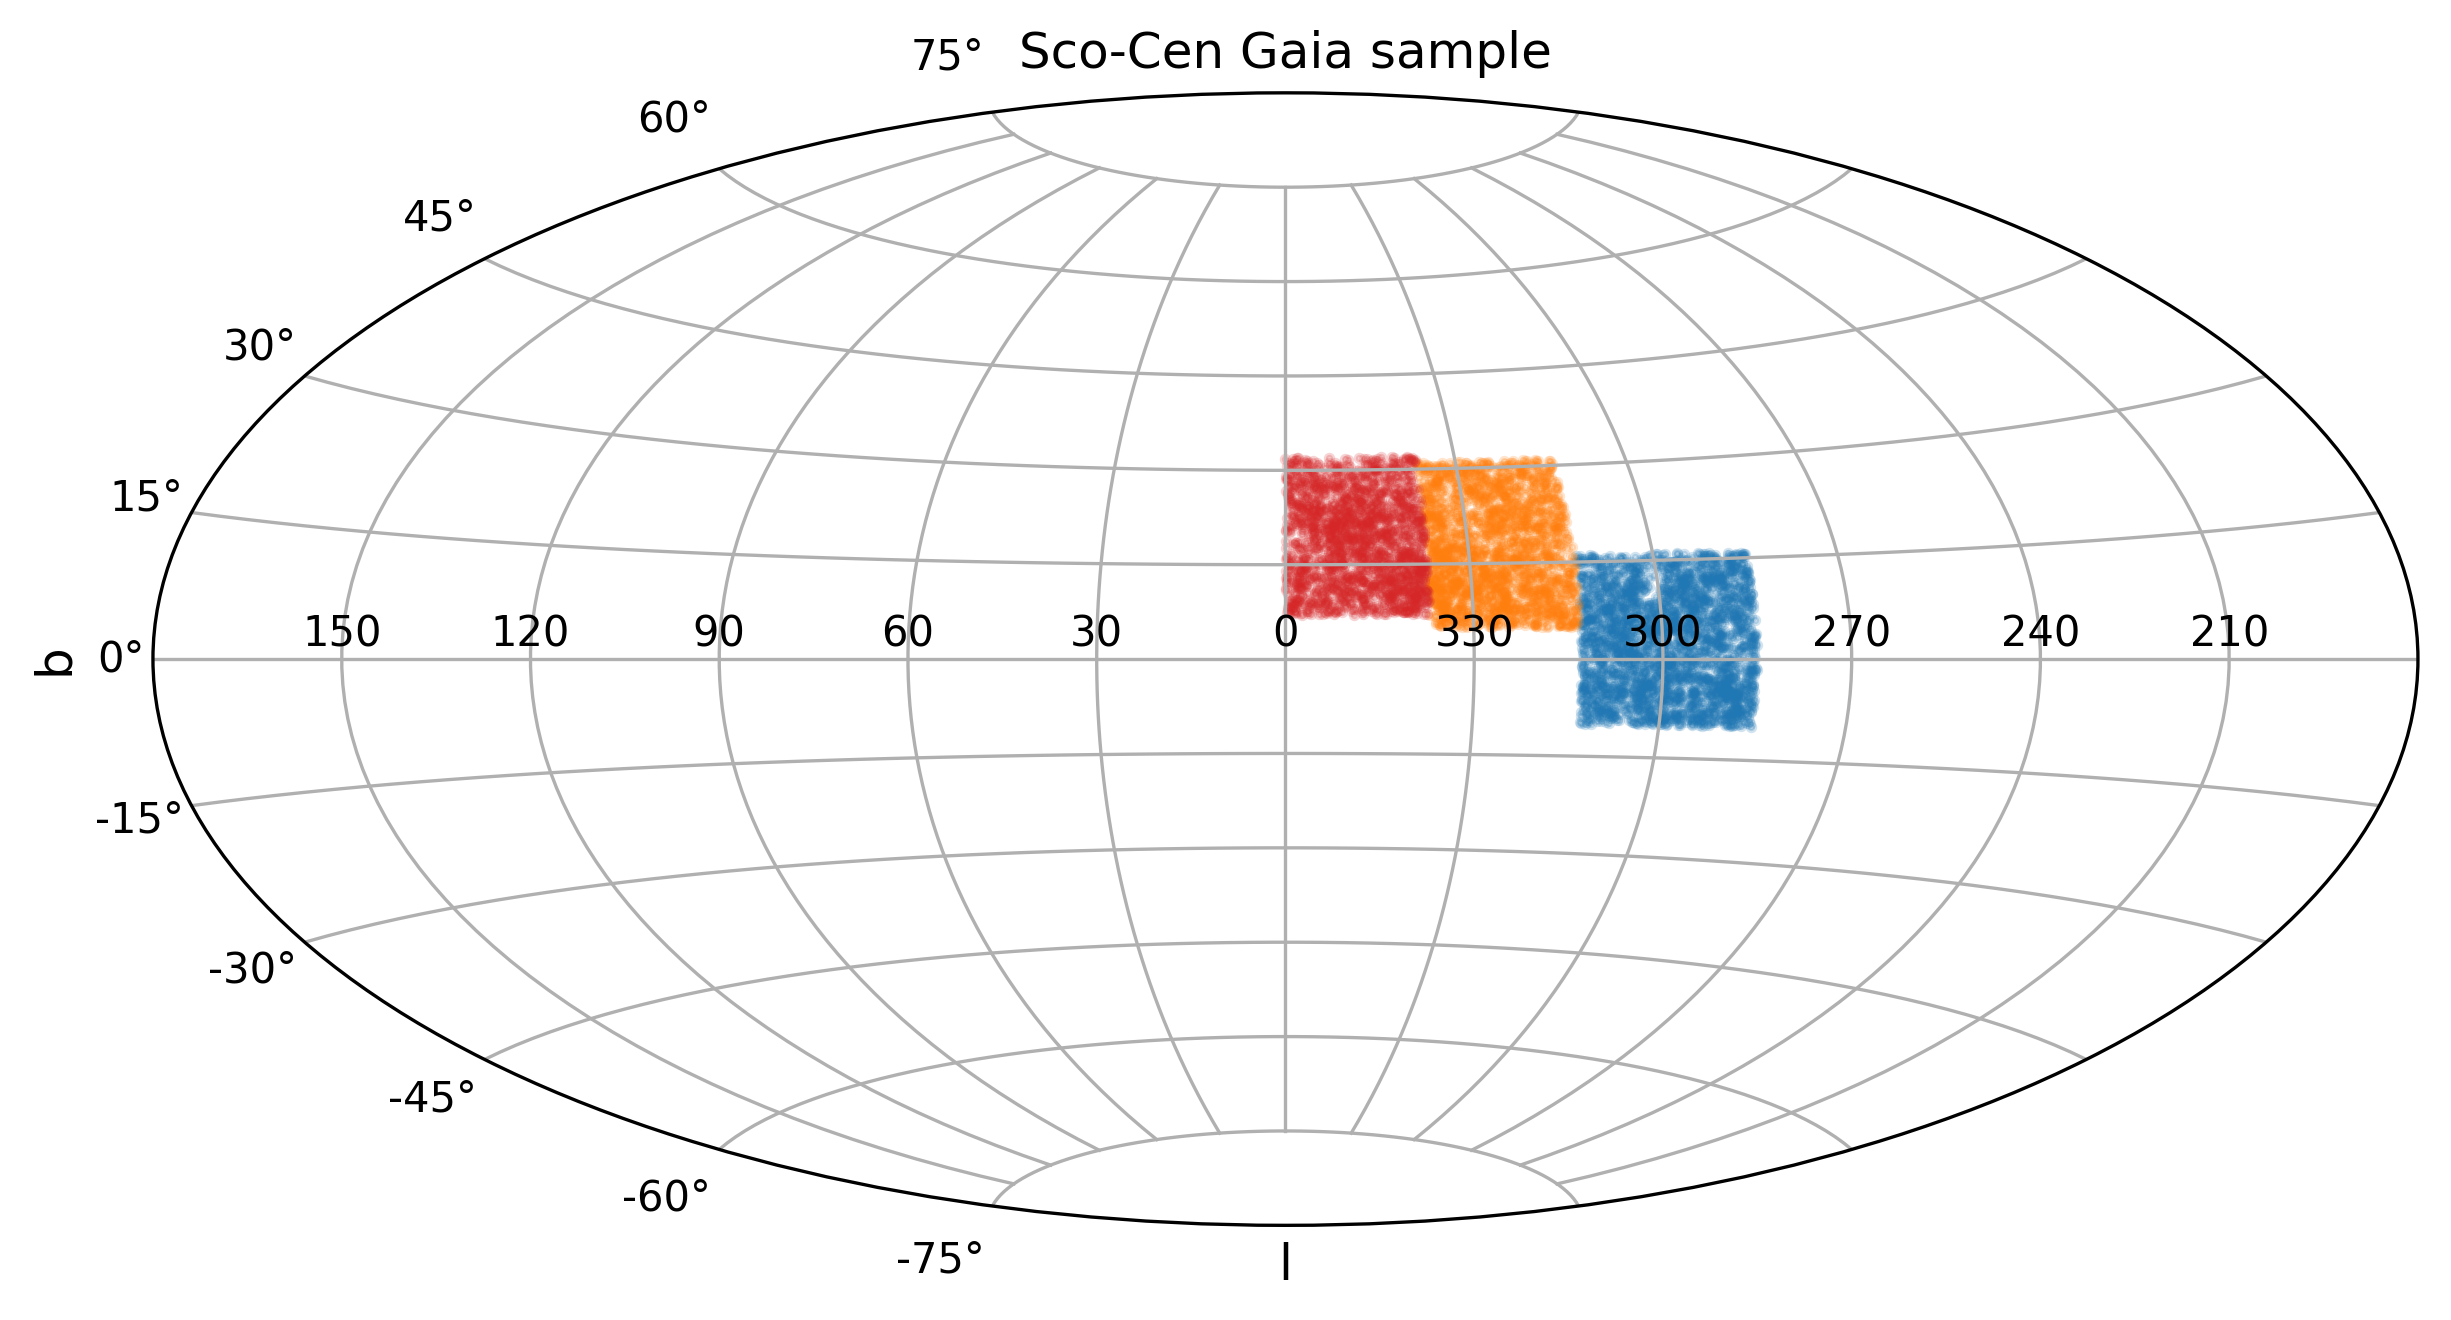
\includegraphics[width = 16cm, height = 8cm]{./Graficos/Capitulo_3/5_Sco-Cen/Sco_Cen_Projection_flipped.png}} 
\caption{\scriptsize{ScoCen subgroups position in galactic coordinates. Each subgroup LCC (blue), UCL (orange) and US (red), contains the initial sample of stars as obtained from DR1 in galactic longitude and galactic latitude. The region covers $\sim 90$-degrees in longitude and $\sim 50$-degrees in latitude.}}
\label{fig:Projection_ScoCen}
\end{figure}

This cut-off in proper motion and parallax leads to a new sample of LCC $= 1010$, UCL $= 746$, and US $= 797$ stars respectively, in which we have ruled out stars which certainly do not belong to the association. The next step is to narrow down the sample based on the stellar evolution of the cluster. This was performed using evolutionary tracks in which we aimed to use low-mass stars as they are the ones with higher probabilities of exoplanetary rings transits as shown before, and also using isochrones to restrict each sample to contain the young population. %This is thoroughly explained in \autoref{sec:SEM_1}.   


%============================================================================================================================================================

\section{Stellar Evolution Models} \label{sec:SEM_1}

The highest transit probability was obtained for low-mass stars. As shown in \autoref{fig:Rings_Prob}, the probability of detecting rings transiting in front of the parent stars decreases as the stellar mass increases independent of the lifetime for the planetary rings which only causes a vertical shift i.e. a change in the total expected number of transits. Therefore, it is important to select a reliable sample of stars in ScoCen which can lead to a high chance of detecting this kind of transits. The first step consisted in taking the sample mentioned above in which a cut-off in the dynamics and distance for the association has been applied, and run different stellar track models with an initial value of extinction $\textnormal{A}_\textnormal{v} = 0$ for each sub-region using the \textit{MIST}-package. In \autoref{fig:Stellar_Tracks_1}, the color-magnitude diagram for each sub-region is presented for $\textnormal{G}$- and $\textnormal{K}_\textnormal{s}$-bands. The magnitudes were obtained using \textit{Gaia}-DR1 and transformed to the absolute magnitude (see \autoref{ch:Appendix}). The color index was computed using a cross-match identification of the sources in \textit{Gaia}-DR1 with \textit{The Two Micron All-Sky Survey} (2MASS) tables. The stellar tracks shown correspond to stellar masses from $0.5 \textnormal{M}_\odot$ to  $2.1 \textnormal{M}_\odot$ in steps of $0.4 \textnormal{M}_\odot$, which were computed for the required photometric bands in \textit{Gaia} and \textit{2MASS}. Although each sub-region shows different spread, the stars seem to be distributed mostly below the $1.3 \textnormal{M}_\odot$ stellar track. Therefore, no-extra cut-off in mass in needed because if one compares to \autoref{fig:Rings_Prob} the highest probabilities are for stars $< 2.0 \textnormal{M}_\odot$. The same conditions were assumed to compute the isochrones shown in \autoref{fig:Isochrones_1}. Each figure corresponds to the LCC, UCL, and US color-magnitude diagrams with isochrones of $5, 15, 20, 30$ and $60$-Myr. The upper isochrone is the youngest ($5$-Myr) while the lower represents the oldest ($60$-Myr). In each of the three cases, most of the stars are contained in between the youngest and the oldest isochrones. It is useful to have in mind that all the isochrones are computed without extinction. A few stars lie outside the isochrones delimited region, thus, the idea is to use the isochrones to just select those stars that satisfy the absolute magnitude $\textnormal{M}_\textnormal{G}$ and color index $\textnormal{G} - \textnormal{K}_\textnormal{s}$ conditions in between both isochrones. After selecting only those stars in between the isochrones the final sample is reduced to LCC $= 868$, UCL $= 633$, and US $= 649$ stars respectively (see \autoref{fig:Isochrones_2} for the initial distribution of stars). For comparison in \autoref{ch:Appendix}, \autoref{sec:Sample_Selection_1}, it is shown the original sample of stars without performing the proper motion and parallax cut-off in color index versus the sample after using \cauthor{2016MNRAS.461..794P} (\citeyear{2016MNRAS.461..794P}) constraints in black-dots for each sub-region in \autoref{fig:Stellar_Tracks_1_appendix} and \autoref{fig:Isochrones_1_appendix}.\\       

\begin{figure}[!ht]
\centering
  \subfloat{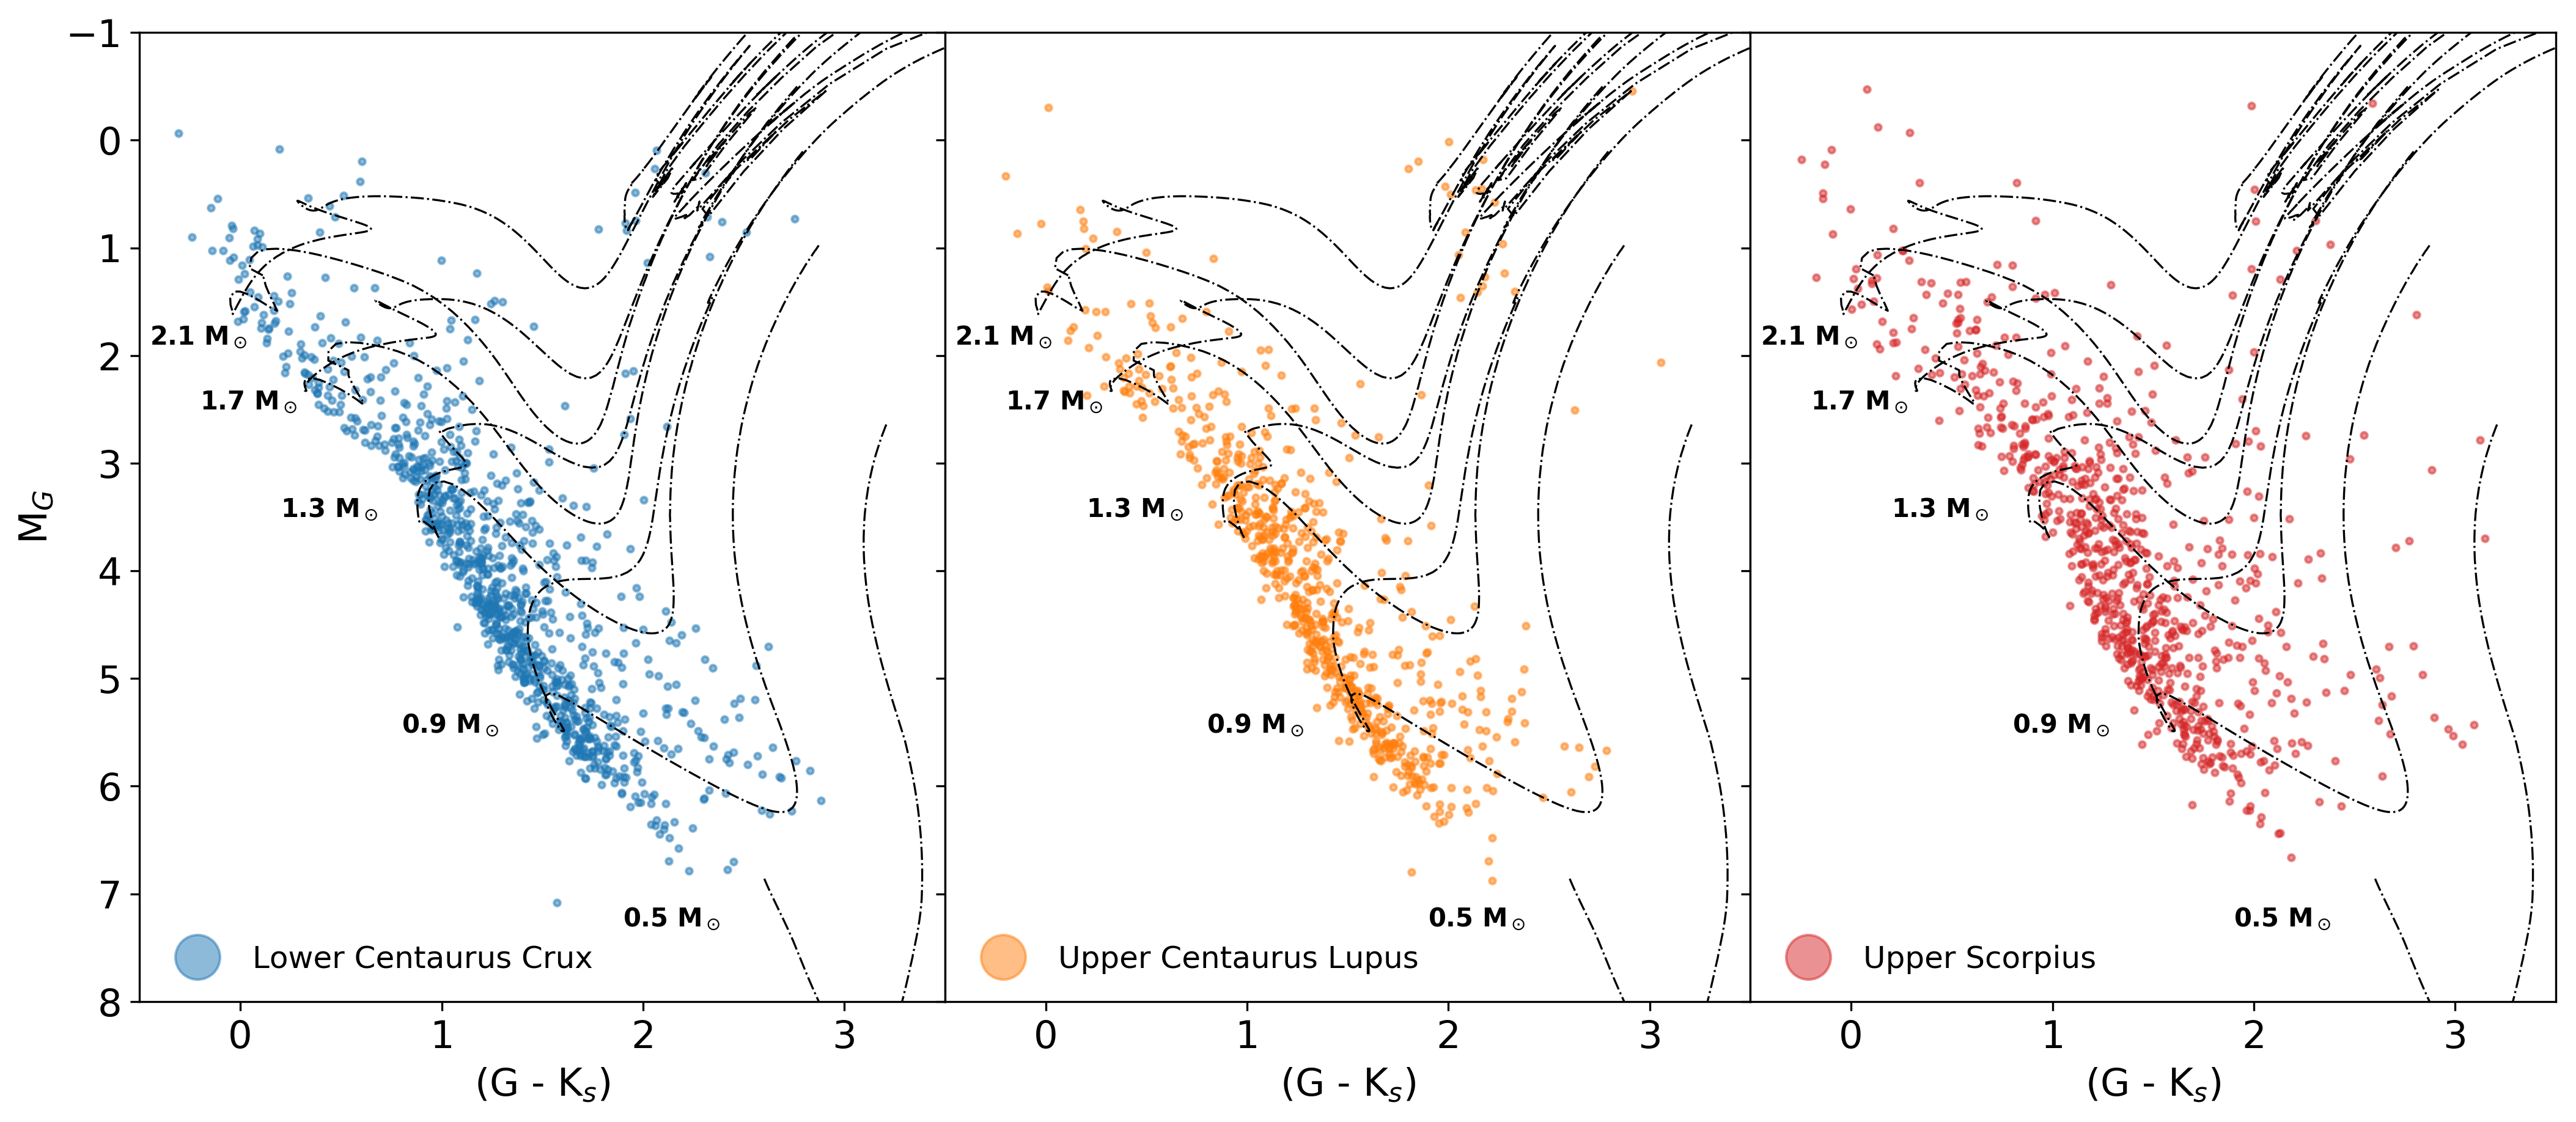
\includegraphics[width = 16cm, height = 8cm]{./Graficos/Capitulo_3/5_Sco-Cen/Mag_Col_diagram_4_2.png}} 
\caption{\scriptsize{Color-magnitude diagrams for each subgroup in ScoCen using \textit{Gaia}-DR1 data. \textit{\textbf{Left}}: LCC stars after the dynamical and positional cuts are shown in blue. The black lines correspond to different stellar tracks. \textit{\textbf{Center}}: UCL stars after the dynamical and positional cuts are shown in orange. The black lines correspond to different stellar tracks. \textit{\textbf{Right}}: US stars after the dynamical and positional cuts are shown in red. The black lines correspond to different stellar tracks. In general for each subgroup, a stellar mass range of $0.5 \textnormal{M}_\odot < \textnormal{M} < 2.1 \textnormal{M}_\odot$ was used along with $\textnormal{A}_\textnormal{v} = 0$ using the \textit{MIST}-package (\cauthor{2016ApJS..222....8D} \citeyear{2016ApJS..222....8D}; \cauthor{2016ApJ...823..102C} \citeyear{2016ApJ...823..102C}).}}
\label{fig:Stellar_Tracks_1}
\end{figure}

\begin{figure}[!ht]
\centering
  \subfloat{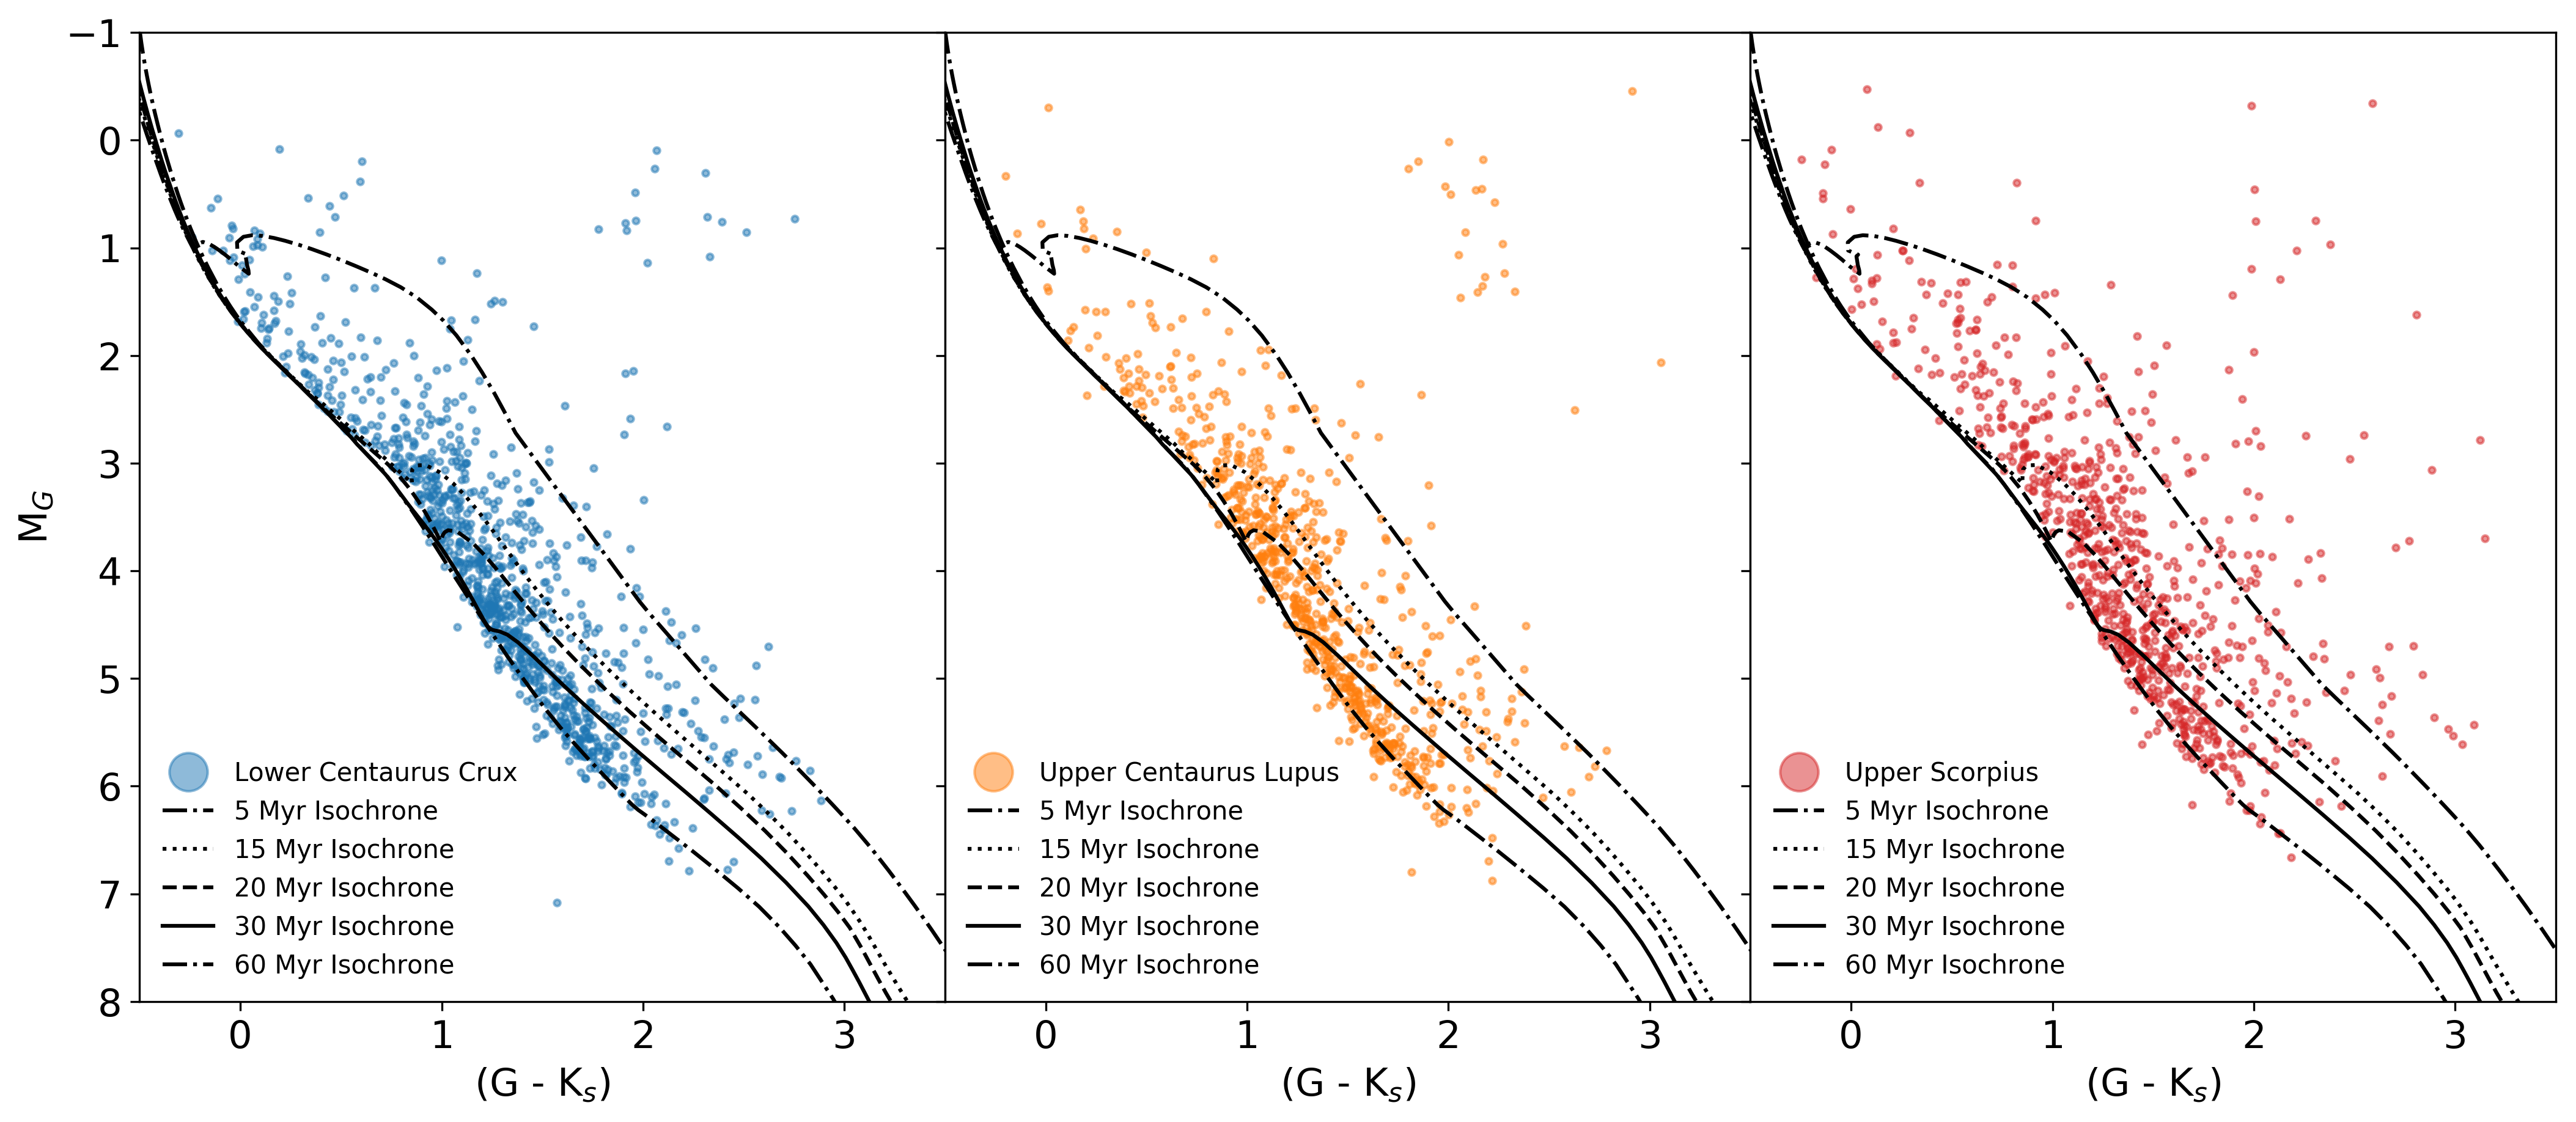
\includegraphics[width = 16cm, height = 8cm]{./Graficos/Capitulo_3/5_Sco-Cen/Mag_Col_diagram_3_Extintion_cut.png}} 
\caption{\scriptsize{Color-magnitude diagrams for each subgroup in ScoCen using \textit{Gaia}-DR1 data. \textit{\textbf{Left}}: LCC stars after the dynamical and positional cuts are shown in blue. The black lines correspond to different isochrones. \textit{\textbf{Center}}: UCL stars after the dynamical and positional cuts are shown in orange. The black lines correspond to different isochrones. \textit{\textbf{Right}}: US stars after the dynamical and positional cuts are shown in red. The black lines correspond to different isochrones. In general for each subgroup, isochrones from $5 \textnormal{Myr}$ to $60 \textnormal{Myr}$ were calculated along with $\textnormal{A}_\textnormal{v} = 0$ using the \textit{MIST}-package (\cauthor{2016ApJS..222....8D} \citeyear{2016ApJS..222....8D}; \cauthor{2016ApJ...823..102C} \citeyear{2016ApJ...823..102C}). The $60 \textnormal{Myr}$ isochrone fits well the main-sequence and the $5 \textnormal{Myr}$ isochrones gives a good range to pre-select young stars.}}
\label{fig:Isochrones_1}
\end{figure}

% \begin{figure}[!ht]
% \centering
%   \subfloat{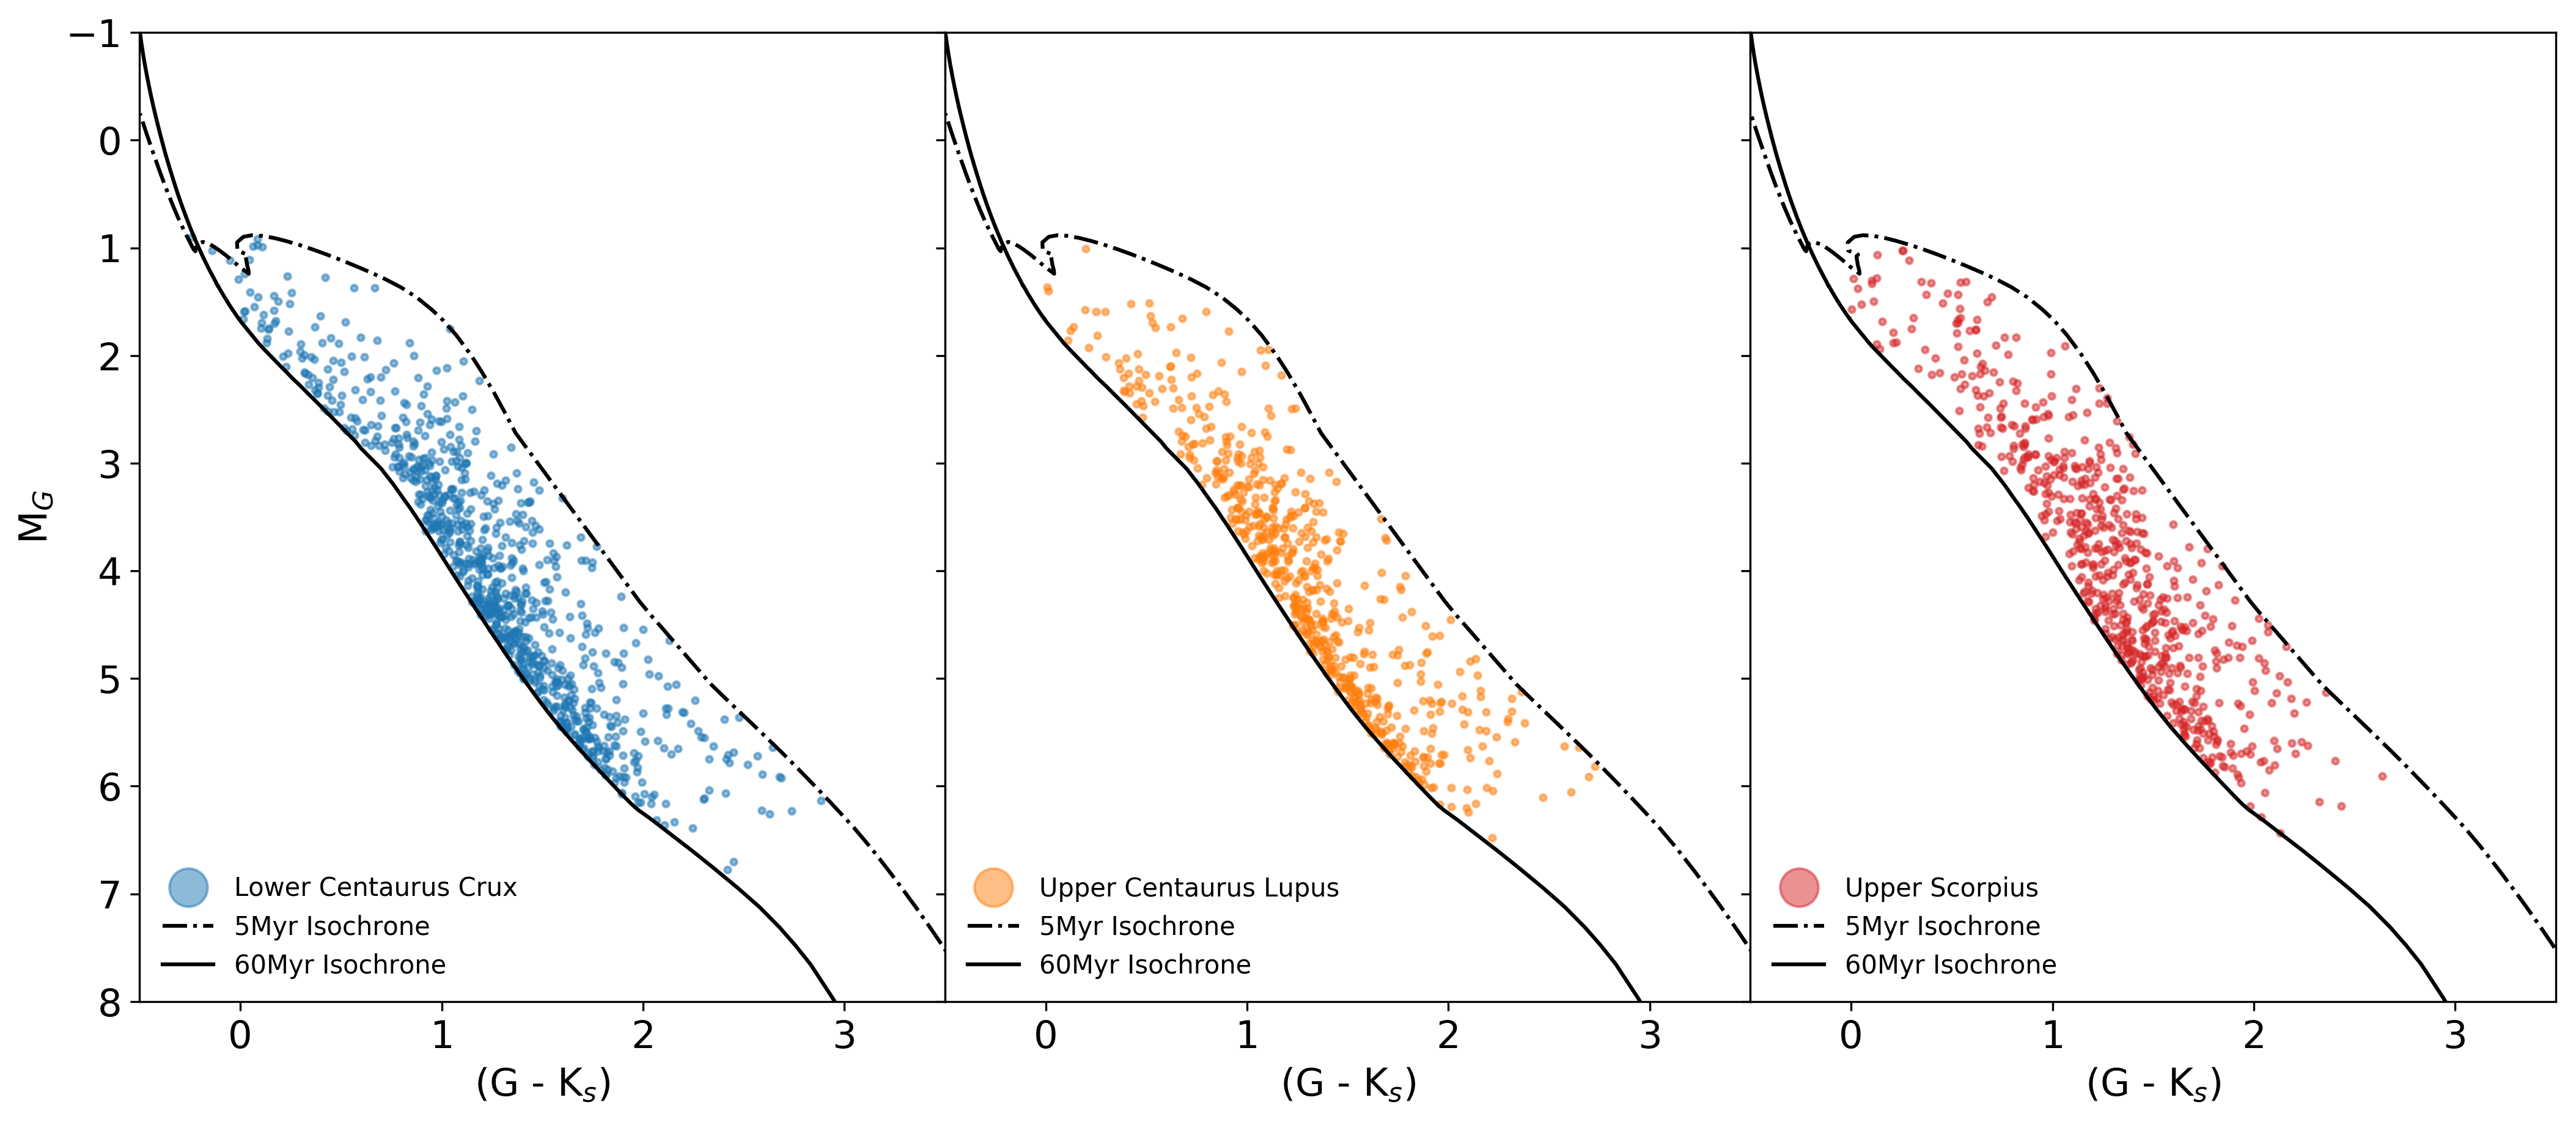
\includegraphics[width = 16cm, height = 8cm]{./Graficos/Capitulo_3/5_Sco-Cen/final_Sample_SCOCEN_Original.png}} 
% \caption{\scriptsize{Color-magnitude diagrams for each subgroup in ScoCen using selected \textit{Gaia}-DR1 data between two different isochrones. \textit{Left}: LCC stars after the dynamical and positional cuts are shown in blue. The black lines correspond to different isochrones. \textit{Center}: UCL stars after the dynamical and positional cuts are shown in orange. The black lines correspond to different isochrones. \textit{Right}: US stars after the dynamical and positional cuts are shown in red. The black lines correspond to different isochrones. Only the $5 \textnormal{Myr}$ to $60 \textnormal{Myr}$ isochrones were used with $\textnormal{A}_\textnormal{v} = 0$ to restrict the sample of stars to be inside this particular region. Following this, stars inside the region are quite likely to belong to the cluster and be in an stellar age range suitable for our study.}}
% \label{fig:Isochrones_2}
% \end{figure}

Besides this, if we want to obtain a reliable sample of stars which belong to ScoCen, we need to include the extinction in each sub-region when computing the stellar tracks and isochrones. As can be seen from \autoref{fig:Isochrones_1}, the $60$-Myr gently touches the main-sequence of this association, thus, it seems legit to compute this isochrone with $\textnormal{A}_\textnormal{v} = 0$ because extinction will shift the isochrones downwards and to the red side of the Hertzsprung-Russell diagram where stars appear fainter and redder. However, in the case of the $5$-Myr isochrone, if we include extinction, then the isochrone will shift upwards including more stars that could be ruled out by our first selection method. Therefore, we proceed to compute the $5$-Myr isochrone including the extinction factor. Based on observations made by \cauthor{1989A&A...216...44D} (\citeyear{1989A&A...216...44D}), we were able to calculate the average, median and $90$-percentile extinction values for each sub-region. In the case of LCC, a total number of 41 stars were used, while for UCL and US, 141 and 100 stars, respectively. In \autoref{fig:SCOCEN_Extinction}, the histograms for each sub-region are shown along with the average, median, and $90$-percentile extinction values. In the case of LCC and UCL, the values are always quite similar, but in the case of US, the values are significantly higher which may affect more drastically the isochrones and stellar tracks in comparison to the other two sub-regions. The values obtained for the average, are in agreement with values reported by \cauthor{2018MNRAS.tmp..210W} (\citeyear{2018MNRAS.tmp..210W}) and are well correlated with the distribution of the dust, as seen in the IRAS $100 \mu \textnormal{m}$ map \cauthor{1989A&A...216...44D} (\citeyear{1989A&A...216...44D}). These values are $0.23$, $0.17$, and $0.76$ for LCC, UCL, and US, respectively.\\     

\begin{figure}[!ht]
\centering
  \subfloat{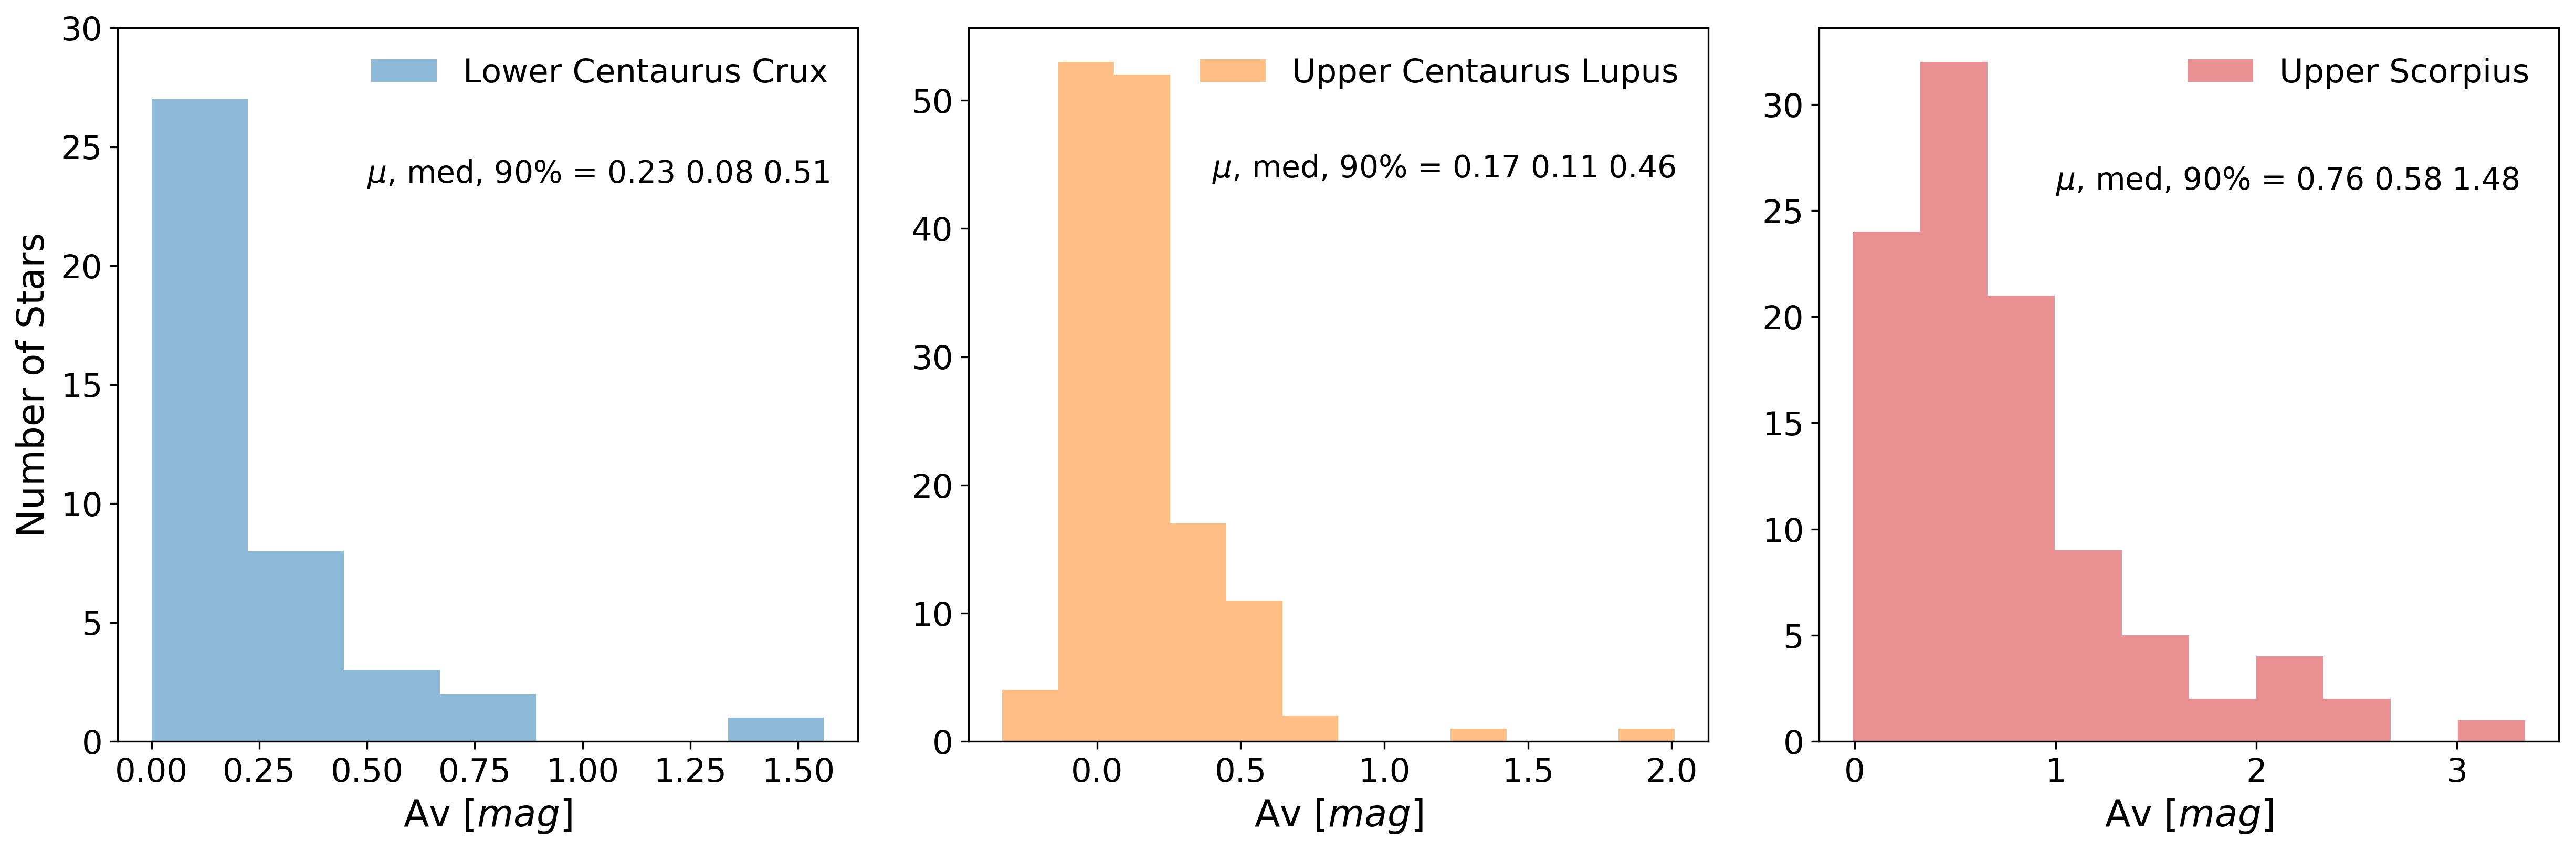
\includegraphics[width = 15.5cm, height = 5.5cm]{./Graficos/Capitulo_3/5_Sco-Cen/Av_histograms.png}} 
\caption{\scriptsize{Histograms corresponding to the number of stars as a function of extinction for each subgroup in ScoCen. Each one of the subgroups LCC, UCL, and US, contains a sample of stars reported in \cauthor{1989A&A...216...44D} (\citeyear{1989A&A...216...44D}) with measured extinction. The mean, median, and $90\%$-percentile are shown. \textit{Upper Scorpius} has the highest extinction value, while \textit{Lower Centaurus-Crux} and \textit{Upper Centaurus-Lupus} both have close extinction values.}}
\label{fig:SCOCEN_Extinction}
\end{figure}

On top of that, the $5$-Myr isochrone was computed using the average extinction values reported above to perform the selection of stars in the color-magnitude diagrams once more. As can be seen in \autoref{fig:Isochrones_3}, the shape of the $5$-Myr isochrone when introducing the extinction factor changes dramatically, increasing the number of stars affected by extintion in our selection i.e. redder and fainter ones. The same happens to LCC and UCL but in a less proportion. However, it is worth noting that the isochrones do not cross each other around $\textnormal{M}_\textnormal{G} \sim 1.0~[\textnormal{mag}]$ as was the case shown in \autoref{fig:Isochrones_1}, allowing for brighter stars to be selected in our sample. If we center our view in the stellar tracks, it is evident from \autoref{fig:Stellar_Tracks_3} that there exists a displacement downwards. However, as stars above $2.1 \textnormal{M}_\odot$ are not a lot, and this does not change that much, we will not perform any cut in stellar mass but we will just cut in stellar age using the isochrones. The new cut and final sample using the isochrones in which the youngest isochrone is affected by extinction is shown in \autoref{fig:Isochrones_4}.\\ 

\begin{figure}[!ht]
\centering
  \subfloat{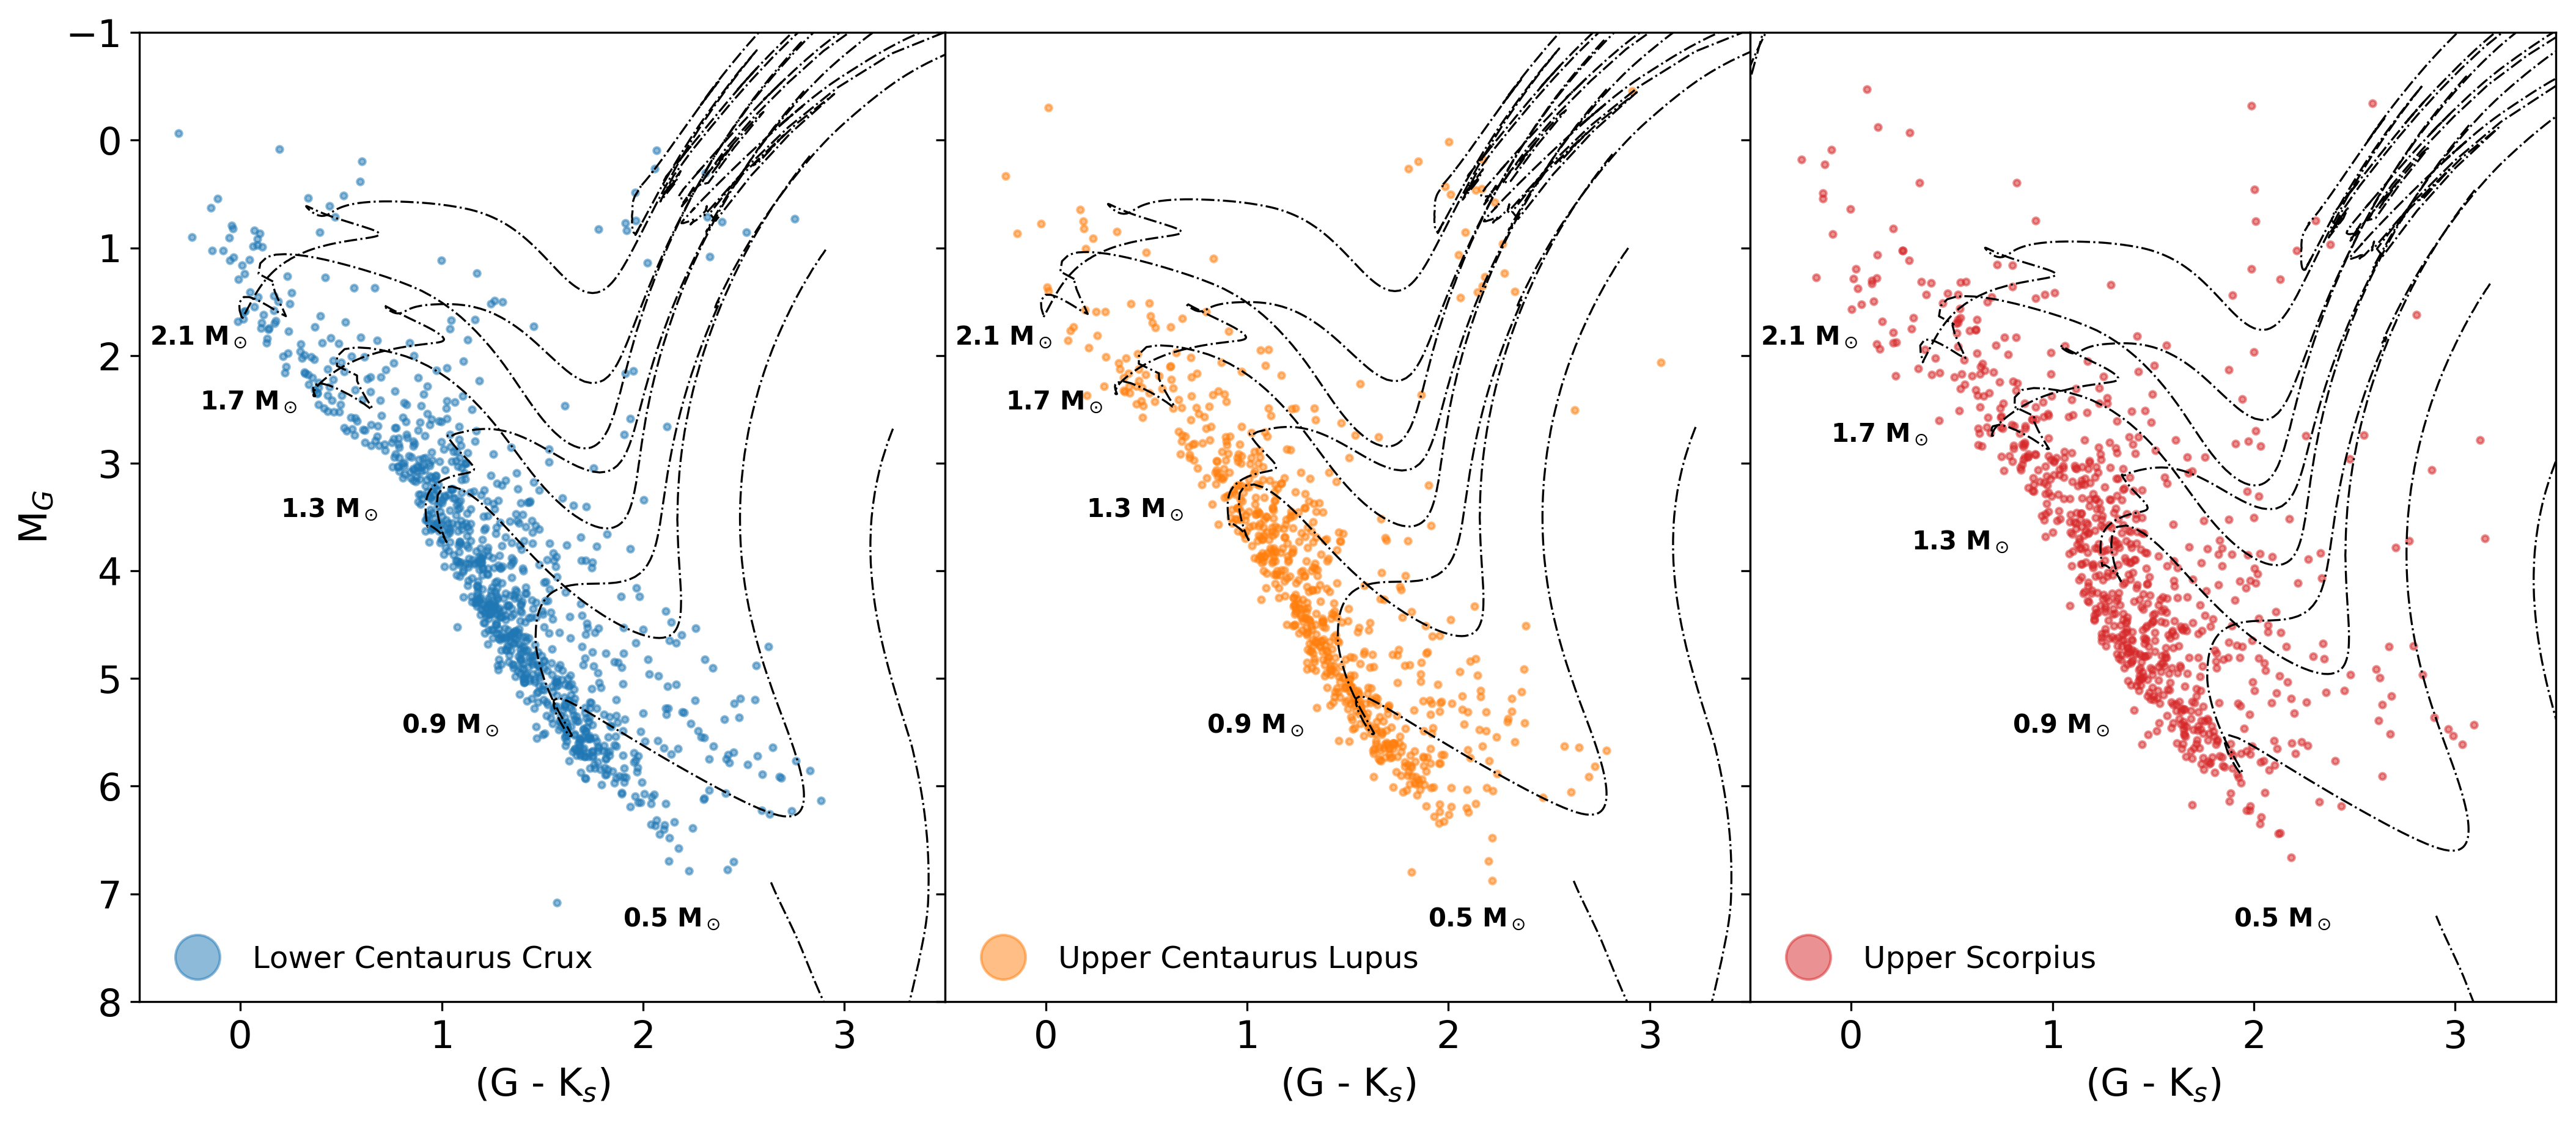
\includegraphics[width = 16cm, height = 8cm]{./Graficos/Capitulo_3/5_Sco-Cen/Mag_Col_diagram_4_Extintion_1.png}} 
\caption{\scriptsize{Color-magnitude diagrams for each subgroup in ScoCen using \textit{Gaia}-DR1 data as in \autoref{fig:Stellar_Tracks_1}, along with stellar tracks using the extinction value measured proposed by \cauthor{1989A&A...216...44D} (\citeyear{1989A&A...216...44D}). \textit{\textbf{Left}}: LCC stars after the dynamical and positional cuts are shown in blue. The black lines correspond to different stellar tracks. \textit{\textbf{Center}}: UCL stars after the dynamical and positional cuts are shown in orange. The black lines correspond to different stellar tracks. \textit{\textbf{Right}}: US stars after the dynamical and positional cuts are shown in red. The black lines correspond to different stellar tracks. In general for each subgroup, a stellar mass range of $0.5 \textnormal{M}_\odot < \textnormal{M} < 2.1 \textnormal{M}_\odot$ was used to compute the stellar tracks using the \textit{MIST}-package (\cauthor{2016ApJS..222....8D} \citeyear{2016ApJS..222....8D}; \cauthor{2016ApJ...823..102C} \citeyear{2016ApJ...823..102C}). In this case, the extinction values for LCC, UCL, and US correspond to $\textnormal{A}_\textnormal{v} = 0.23$, $\textnormal{A}_\textnormal{v} = 0.17$, and $\textnormal{A}_\textnormal{v} = 0.76$, respectively.}}
\label{fig:Stellar_Tracks_3}
\end{figure}

\begin{figure}[!ht]
\centering
  \subfloat{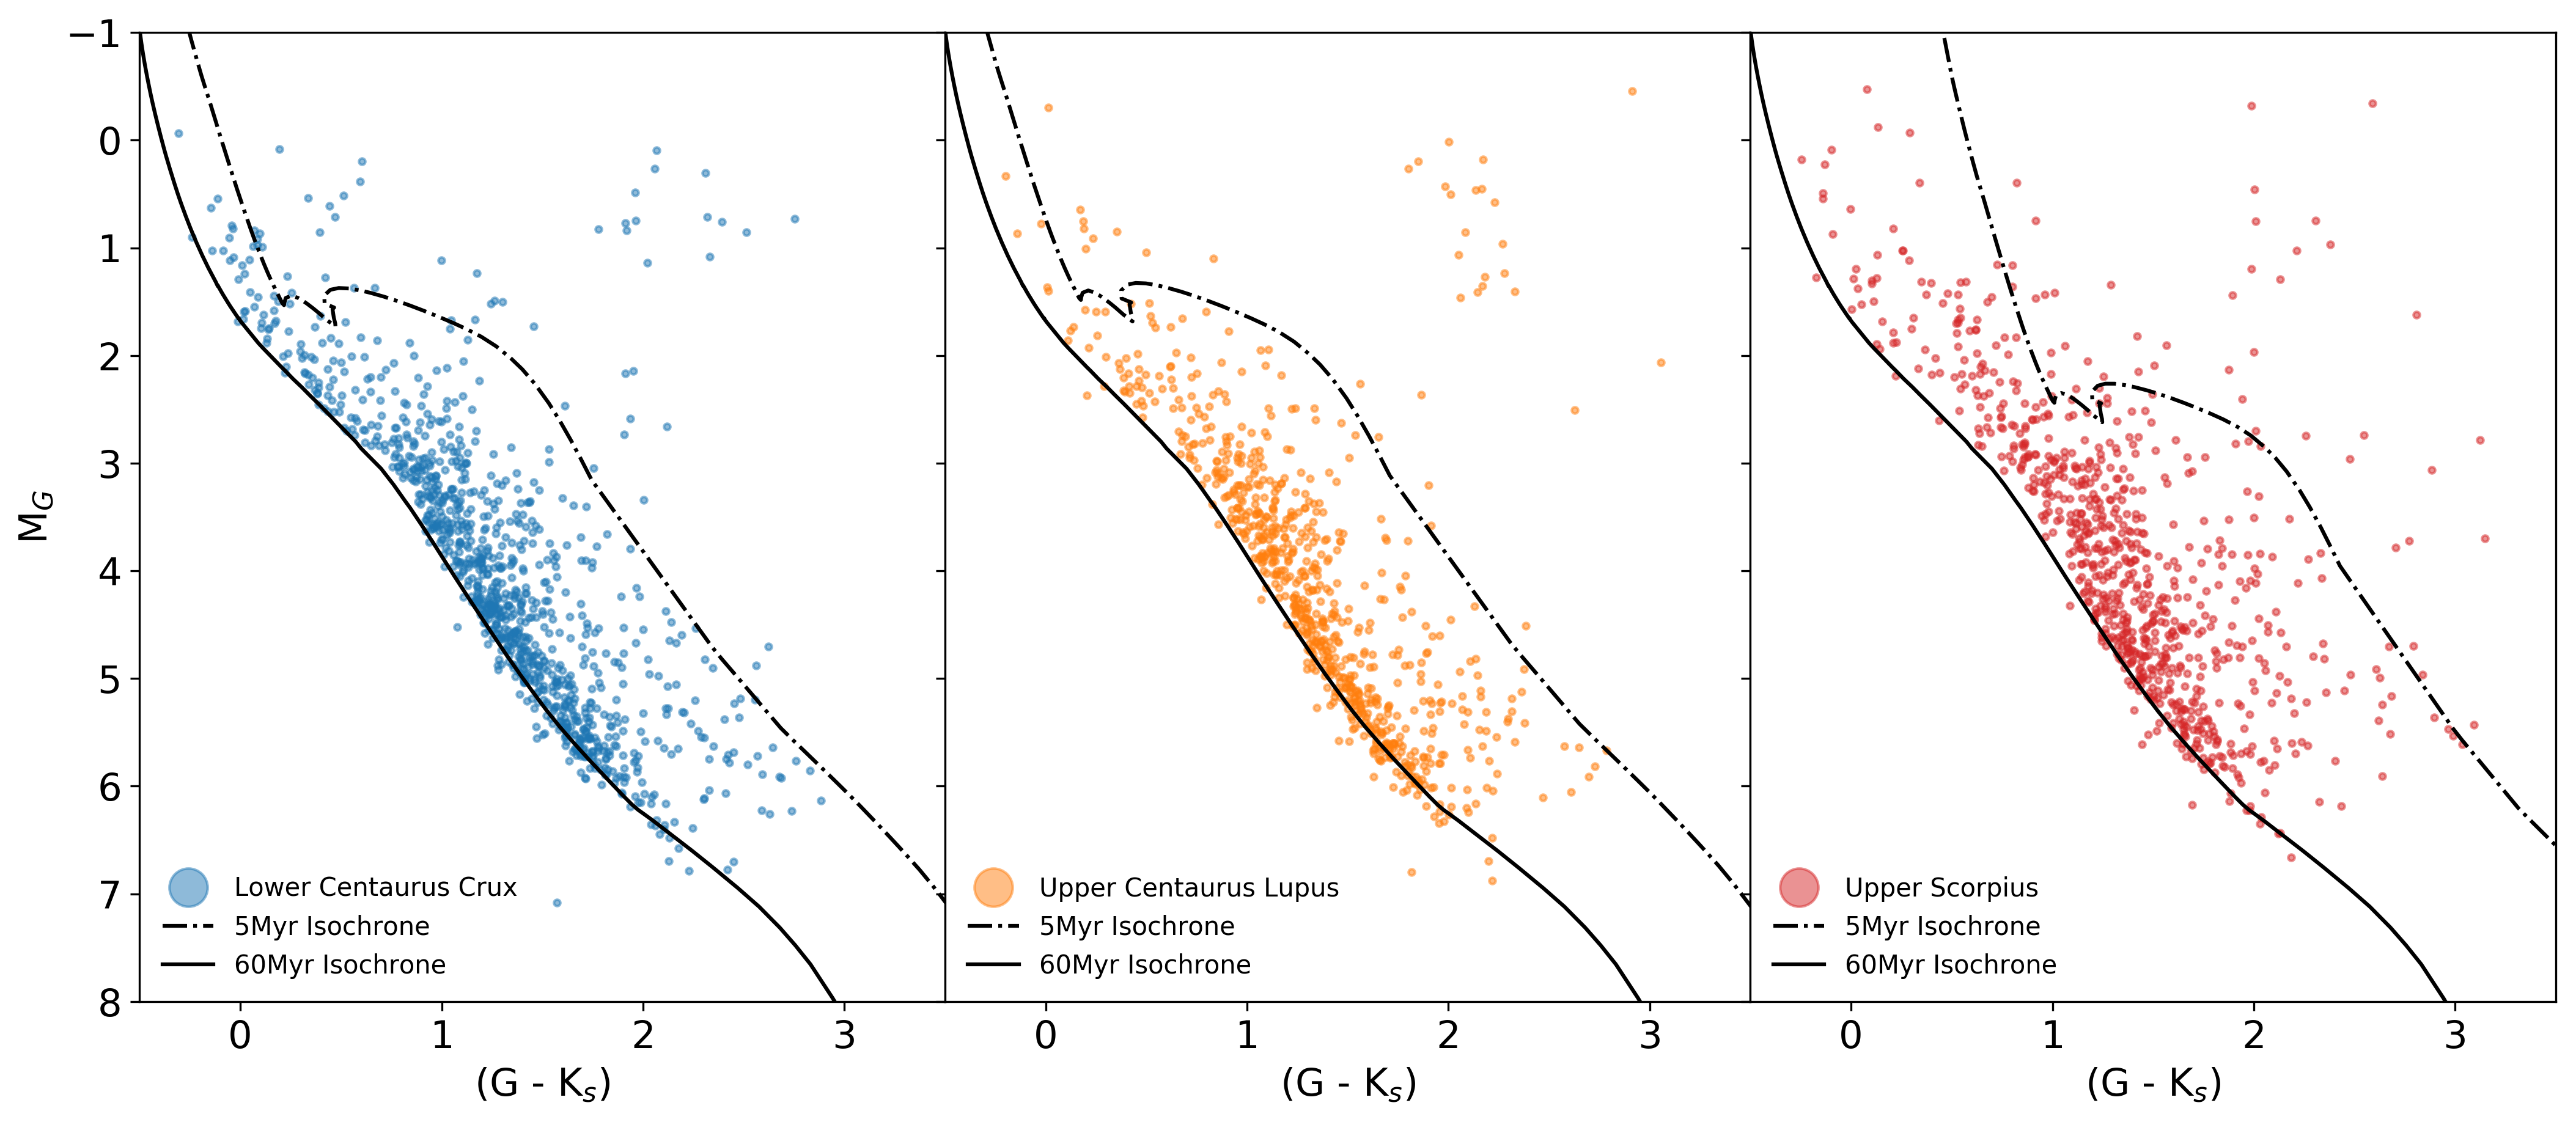
\includegraphics[width = 16cm, height = 8cm]{./Graficos/Capitulo_3/5_Sco-Cen/final_Sample_SCOCEN_2.png}} 
\caption{\scriptsize{Color-magnitude diagrams for each subgroup in ScoCen using \textit{Gaia}-DR1 data as in \autoref{fig:Isochrones_1}, along with isochrones using the extinction value measured proposed by \cauthor{1989A&A...216...44D} (\citeyear{1989A&A...216...44D}). \textit{\textbf{Left}}: LCC stars after the dynamical and positional cuts are shown in blue. The black lines correspond to different isochrones. \textit{\textbf{Center}}: UCL stars after the dynamical and positional cuts are shown in orange. The black lines correspond to different isochrones. \textit{\textbf{Right}}: US stars after the dynamical and positional cuts are shown in red. The black lines correspond to different isochrones. In general for each subgroup, two isochrones $5 \textnormal{Myr}$ and $60 \textnormal{Myr}$ were calculated using the \textit{MIST}-package (\cauthor{2016ApJS..222....8D} \citeyear{2016ApJS..222....8D}; \cauthor{2016ApJ...823..102C} \citeyear{2016ApJ...823..102C}). In this case, the extinction values for LCC, UCL, and US correspond to $\textnormal{A}_\textnormal{v} = 0.23$, $\textnormal{A}_\textnormal{v} = 0.17$, and $\textnormal{A}_\textnormal{v} = 0.76$, respectively.}}
\label{fig:Isochrones_3}
\end{figure}

% \begin{figure}[!ht]
% \centering
%   \subfloat{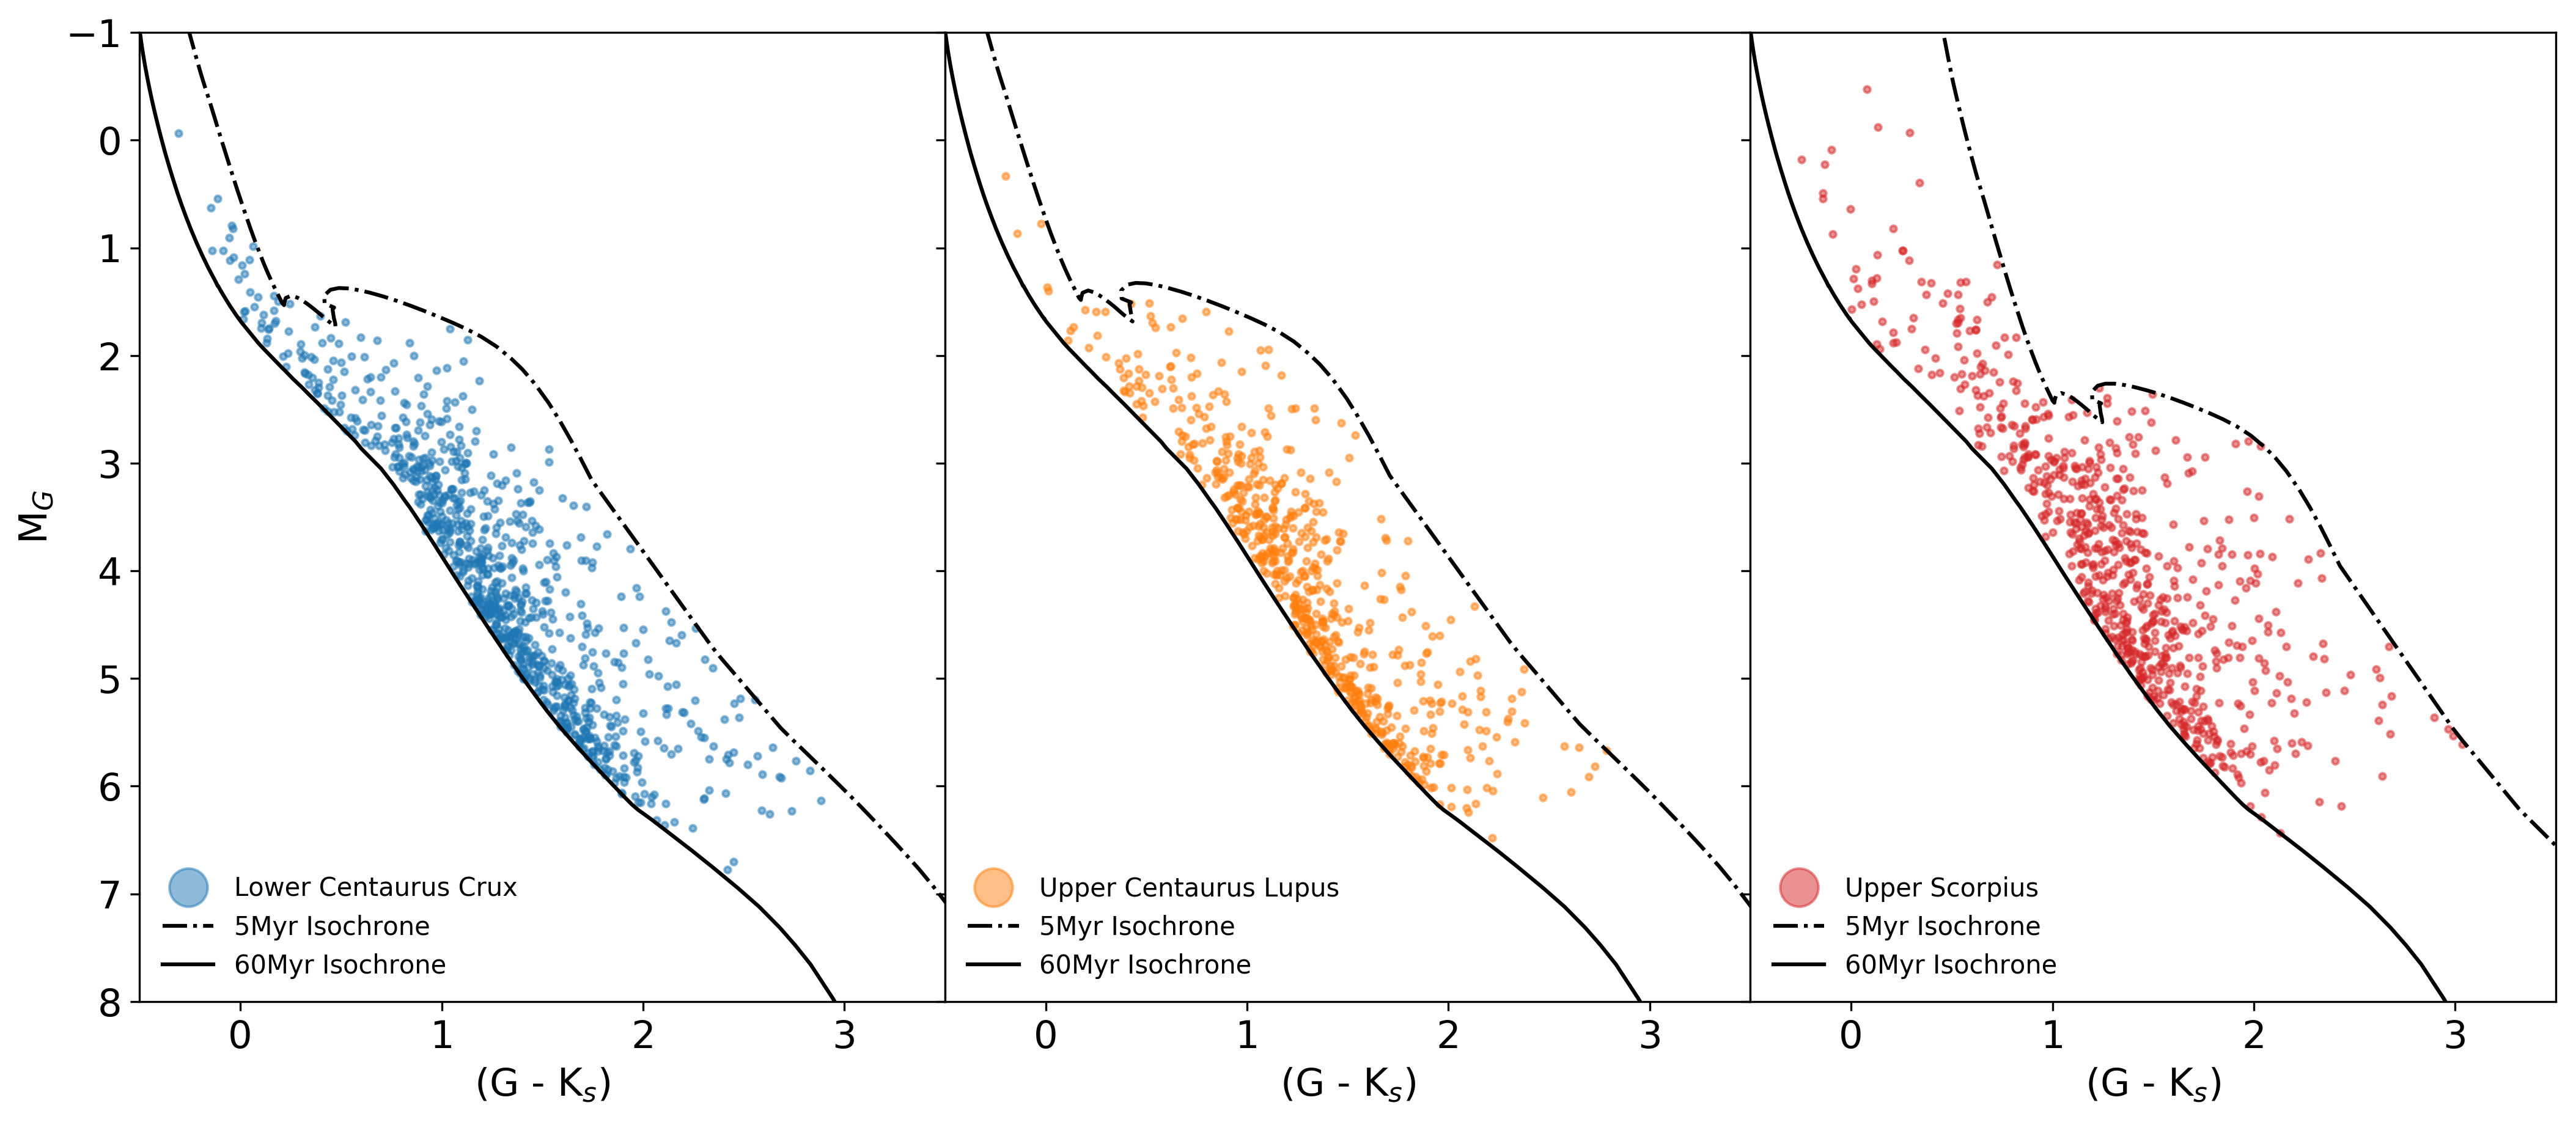
\includegraphics[width = 16cm, height = 8cm]{./Graficos/Capitulo_3/5_Sco-Cen/final_Sample_SCOCEN.png}} 
% \caption{\scriptsize{Color-magnitude diagrams for each subgroup in ScoCen using selected \textit{Gaia}-DR1 data between two different isochrones as in \autoref{fig:Isochrones_2}, along with isochrones using the extinction value measured proposed by \cauthor{1989A&A...216...44D} \citeyear{1989A&A...216...44D}. \textit{Left}: LCC stars after the dynamical and positional cuts are shown in blue. The black lines correspond to different isochrones. \textit{Center}: UCL stars after the dynamical and positional cuts are shown in orange. The black lines correspond to different isochrones. \textit{Right}: US stars after the dynamical and positional cuts are shown in red. The black lines correspond to different isochrones. Only the $5 \textnormal{Myr}$ to $60 \textnormal{Myr}$ isochrones were used to restrict the sample of stars to be inside this particular region. Following this, stars inside the region are quite likely to belong to the cluster and be in an stellar age range suitable for our study. In this case, the extinction values for LCC, UCL, and US correspond to $\textnormal{A}_\textnormal{v} = 0.23$, $\textnormal{A}_\textnormal{v} = 0.17$, and $\textnormal{A}_\textnormal{v} = 0.76$, respectively.}}
% \label{fig:Isochrones_4}
% \end{figure}

The main goal out of this process is to obtain a reliable sample which contains as much as possible stars which could be potential candidates to belong to the ScoCen association based on distance and dynamical properties derived from literature. As was stated before, this analysis was performed on a sample data using \textit{Gaia}-DR1, and the final sample is made of LCC $= 889$, UCL $= 644$, and US $= 705$ stars respectively, in which there is a slight increase in the number of stars per sub-region compared to the case in which no extinction is used as expected because the region between the isochrones is now larger.\\

In the next section, the same process described above to obtain the final sample but using the new data provided through \textit{Gaia}-DR2 is addressed. A few extra steps are needed due to new conditions imposed on parameters as color, parallax, and measurement errors which will be described in order to justify the selected stars which will be cross-matched to the \textit{SuperWASP} database.  

%============================================================================================================================================================

\section{\textit{Gaia}-DR2 Analysis}\label{sec:CleaningProcess}

Resolved or partially resolved binaries cause different kind of errors, for example when the different observations of a source variously refer to one or the other of the components, or to the photocentre, depending on the direction of the scan \cauthor{2018arXiv180409366L} (\citeyear{2018arXiv180409366L}). In some cases, this is known to produce spurious results, for instance, very large positive or negative parallaxes \cauthor{2017A&A...599A..50A} (\citeyear{2017A&A...599A..50A}). \textit{Gaia} DR2 contains a small number of sources with very large positive or negative parallaxes, for example exceeding $\pm 1$ arcsec. These are most likely produced by cross-matching issues, where different observation of the same nominal source is matched to different physical sources \cauthor{2018arXiv180409366L} (\citeyear{2018arXiv180409366L}). In such cases, the proper motion, in general, will also be corrupted. Thus, one must perform an extra clean process on the released data in order to correct for spurious sources and obtain a reliable scientific sample because no filtering was made in the \textit{Gaia} Archive based on the sizes of the parallaxes and proper motions. To perform this corrections and select astrometrically `clean' subsets we followed the method suggested in \textit{Appendix C} of \cauthor{2018arXiv180409366L} (\citeyear{2018arXiv180409366L}) and the main steps are described as follows.\\

The data provided in \textit{Gaia} DR2 satisfy a five-parameter solution which is accepted if the following conditions are met for the source:

\begin{enumerate}[label=(\roman*)]
\item mean magnitude $\textnormal{G} \leq 21.0$
\item \texttt{visibility\_periods\_used} $\geq 6$
\item \texttt{astrometric\_sigma5d\_max} $\leq~(1.2\textnormal{mas})\times\gamma(\textnormal{G})$
\end{enumerate}

where $\gamma(\textnormal{G}) = \textnormal{max}[1, 10^{0.2(G-18)}]$. This criterion was designed to include as many sources as possible with reasonably reliable astrometry \cauthor{2018arXiv180409366L} (\citeyear{2018arXiv180409366L}), though it must not be taken as fixed recipe for selecting sources with the most reliable astrometry, but it may provide useful hints for further exploration. Having said this, we proceeded to select our sample of stars given the parallax/proper motion (see \autoref{sec:GaiaSamples}) and coordinates (see \autoref{tab:ScoCen_SpatialDist}) limits for each one of the subgroups conforming ScoCen, and extra conditions on the parallax and photometry accuracy as given by, 

\begin{enumerate}[label=(\roman*)]
\item galactic coordinates as listed in \autoref{tab:ScoCen_SpatialDist} and parallaxes given in \cauthor{2016MNRAS.461..794P} (\citeyear{2016MNRAS.461..794P})
\item $\varpi/\sigma_\varpi > 10$
\item \texttt{phot\_bp\_mean\_flux\_over\_error} $> 10$
\item \texttt{phot\_rp\_mean\_flux\_over\_error} $> 10$
\end{enumerate}

Nominally, \textit{(i)} selects sources satisfying the galactic coordinates, and parallax and proper motion cuts, \textit{(ii)} those with at most $10\%$ uncertainty in distance (corresponding to $\simeq 0.2 \textnormal{mag}$ in absolute magnitude), and \textit{(iii)}-\textit{(iv)} those with at most $10\%$ uncertainty in the BP and RP fluxes (corresponding to $\simeq 0.1 \textnormal{mag}$ in $\textnormal{G}_\textnormal{BP}$ and $\textnormal{G}_\textnormal{RP}$). Taken at face value, this selection should produce a quite cleaned HR-diagram. However it is reasonable to expect that in most such cases of spurious parallaxes, observations do not fit the single-stellar parallax model very well leading to an increase in the $\chi^2$ affecting the unit weight error, defined as $u = (\chi^2/\nu)^{1/2}$ in \cauthor{2018arXiv180409366L} (\citeyear{2018arXiv180409366L}). The $\chi^2$ is obtained from the \textit{Gaia} Archive and is given as a column named \texttt{astrometric\_chi2\_al}, and $\nu$ represents the degrees of freedom which can be computed as \texttt{astrometric\_n\_good\_obs\_al}$-5$, accounting for the acceptance model described above.\\

In \autoref{fig:LindegrenSelection}, the unit weight error (e.g. $\textnormal{u}^2$; \autoref{eq:WeightError}) is shown as a function of the absolute magnitude in band-G for each one of the three subgroups in ScoCen. \cauthor{2018arXiv180409366L} (\citeyear{2018arXiv180409366L}) considered all the possible stars within $100~\textnormal{pc}$ and realized that a strong rise in $\textnormal{G} < 6$ is caused by uncalibrated CCD saturation; also a blob of moderately large values of $\textnormal{u}$ for $\textnormal{G} > 18$ possibly extending to larger values for brighter sources; and a general scatter of large $\textnormal{u}$ at all magnitudes, possibly caused by partially resolved or astrometric binaries. Thus, if sources with $\textnormal{G} < 6$ which basically includes most of the giants are to be kept while removing the blob at $\textnormal{G} > 18$ the possible cut is given by the square root of \autoref{eq:WeightError}, however, as we have a different sample, we decided to clean without considering the square root. Besides, additional scatter in the Hertzsprung-Russell diagram is produced by photometric errors mainly in the $\textnormal{G}_\textnormal{BP}$ and $\textnormal{G}_\textnormal{RP}$ bands, affecting crowded areas, in particular with faint sources. An indicator of possible issues with the $\textnormal{G}_\textnormal{BP}$ and $\textnormal{G}_\textnormal{RP}$ photometry is given in the \textit{Gaia} DR2 as the flux error factor $\textnormal{E} = (\textnormal{I}_\textnormal{BP} + \textnormal{I}_\textnormal{RP}) / \textnormal{I}_\textnormal{G}$ (\texttt{phot\_bp\_rp\_excess\_factor}), where each $\textnormal{I}_\textnormal{x}$ corresponds to the flux in band $\textnormal{x}$ as shown in \cauthor{2017A&A...600A..51E} (\citeyear{2017A&A...600A..51E}). Following \cauthor{2018arXiv180409366L} (\citeyear{2018arXiv180409366L}), the flux excess can be restricted using $1.0 + 0.015(\textnormal{G}_\textnormal{BP}-\textnormal{G}_\textnormal{RP})^2 < \textnormal{E} < 1.3 + 0.06(\textnormal{G}_\textnormal{BP}-\textnormal{G}_\textnormal{RP})^2$. After all this cleaning process is applied, some scatter still can be present between the main and white-dwarf sequences (see \autoref{fig:FinalSample_DR2}) which could be partly real, consisting of binaries with white-dwarf and main-sequence companions of roughly equal magnitude. Roughly equal number of of positive and negative spurious parallaxes can be present due to different observations of the same \textit{Gaia} source being matched to two (or more) physically distinct objects.

\begingroup
\large
\begin{equation}
  \textnormal{u}^2 = \frac{\chi^2}{\nu} < 1.4 \times \textnormal{max} (~1, \textnormal{exp(~-0.4(~\textnormal{G} - 19.5~)~)}~)
 \label{eq:WeightError}
\end{equation}
\endgroup \\

% \begin{figure}[!ht]
% \centering
%   \subfloat{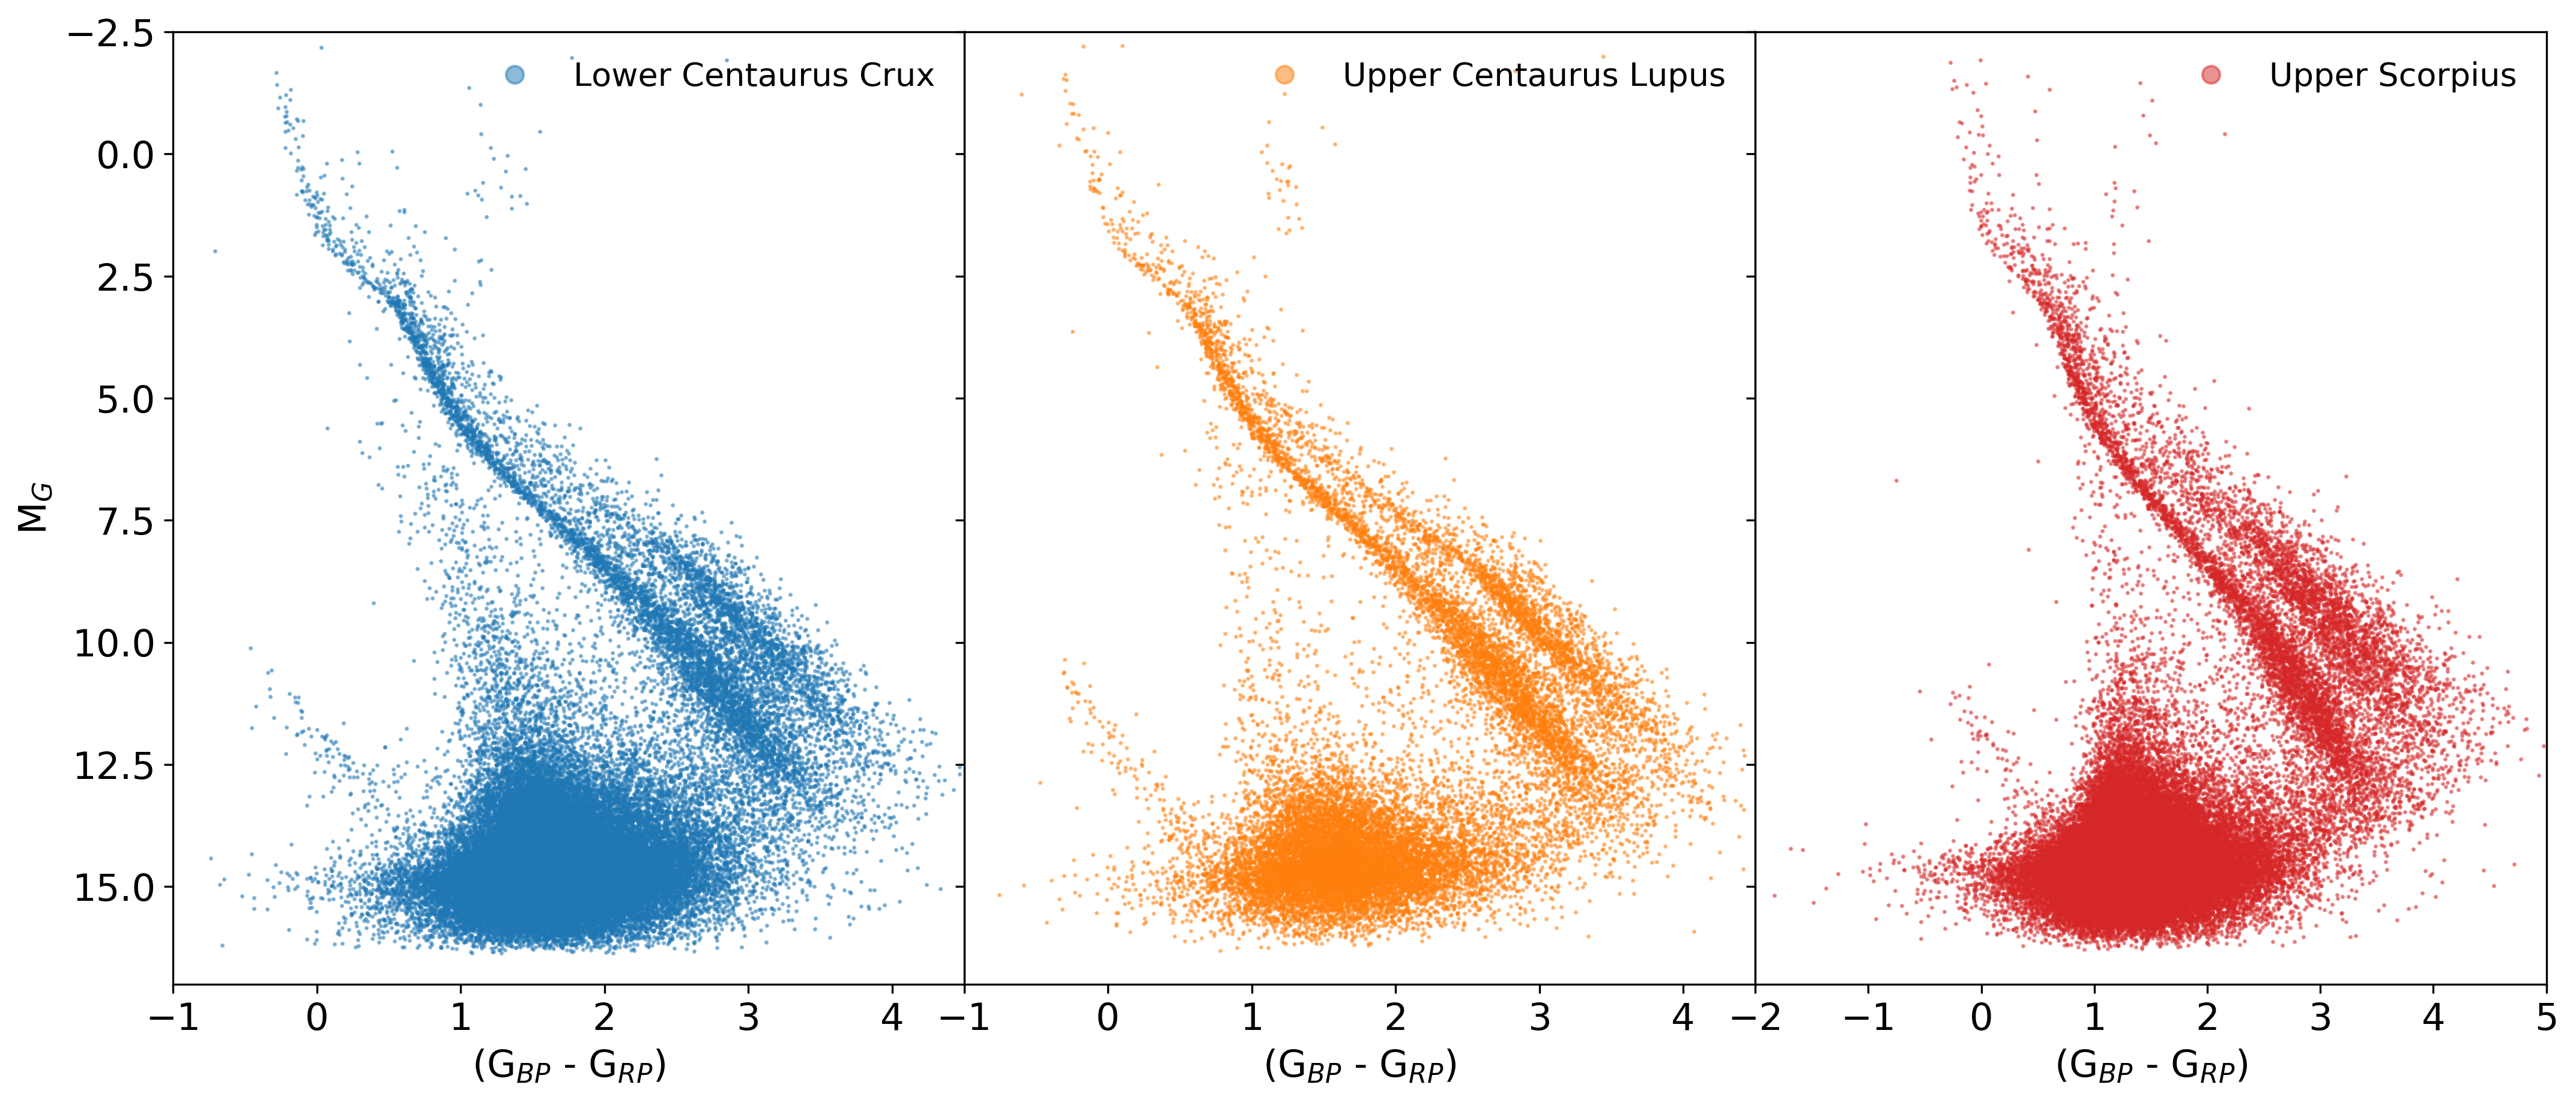
\includegraphics[width = 16cm, height = 7.5cm]{./Graficos/Capitulo_3/7_DR2_LightCurves/DR2_Sample_NoSelection_2_2.png}} 
% \caption{\scriptsize{Color-magnitude diagram using \textit{Gaia}-DR2 data for each subgroup in ScoCen. \textit{Left}: LCC absolute magnitude in the $\textnormal{G}$-band as a function of color-index $\textnormal{G}_\textnormal{BP} - \textnormal{G}_\textnormal{RP}$. \textit{Center}: UCL absolute magnitude in the $\textnormal{G}$-band as a function of color-index $\textnormal{G}_\textnormal{BP} - \textnormal{G}_\textnormal{RP}$. \textit{Right}: US absolute magnitude in the $\textnormal{G}$-band as a function of color-index $\textnormal{G}_\textnormal{BP} - \textnormal{G}_\textnormal{RP}$. In contrast to \textit{Gaia}-DR1, the new data sample contains more stars in each subgroup, and stars with absolute magnitude up to $\textnormal{M}_\textnormal{G} > 17$.}}
% \label{fig:NewData_DR2}
% \end{figure}
% 
% \begin{figure}[!ht]
% \centering
%   \subfloat{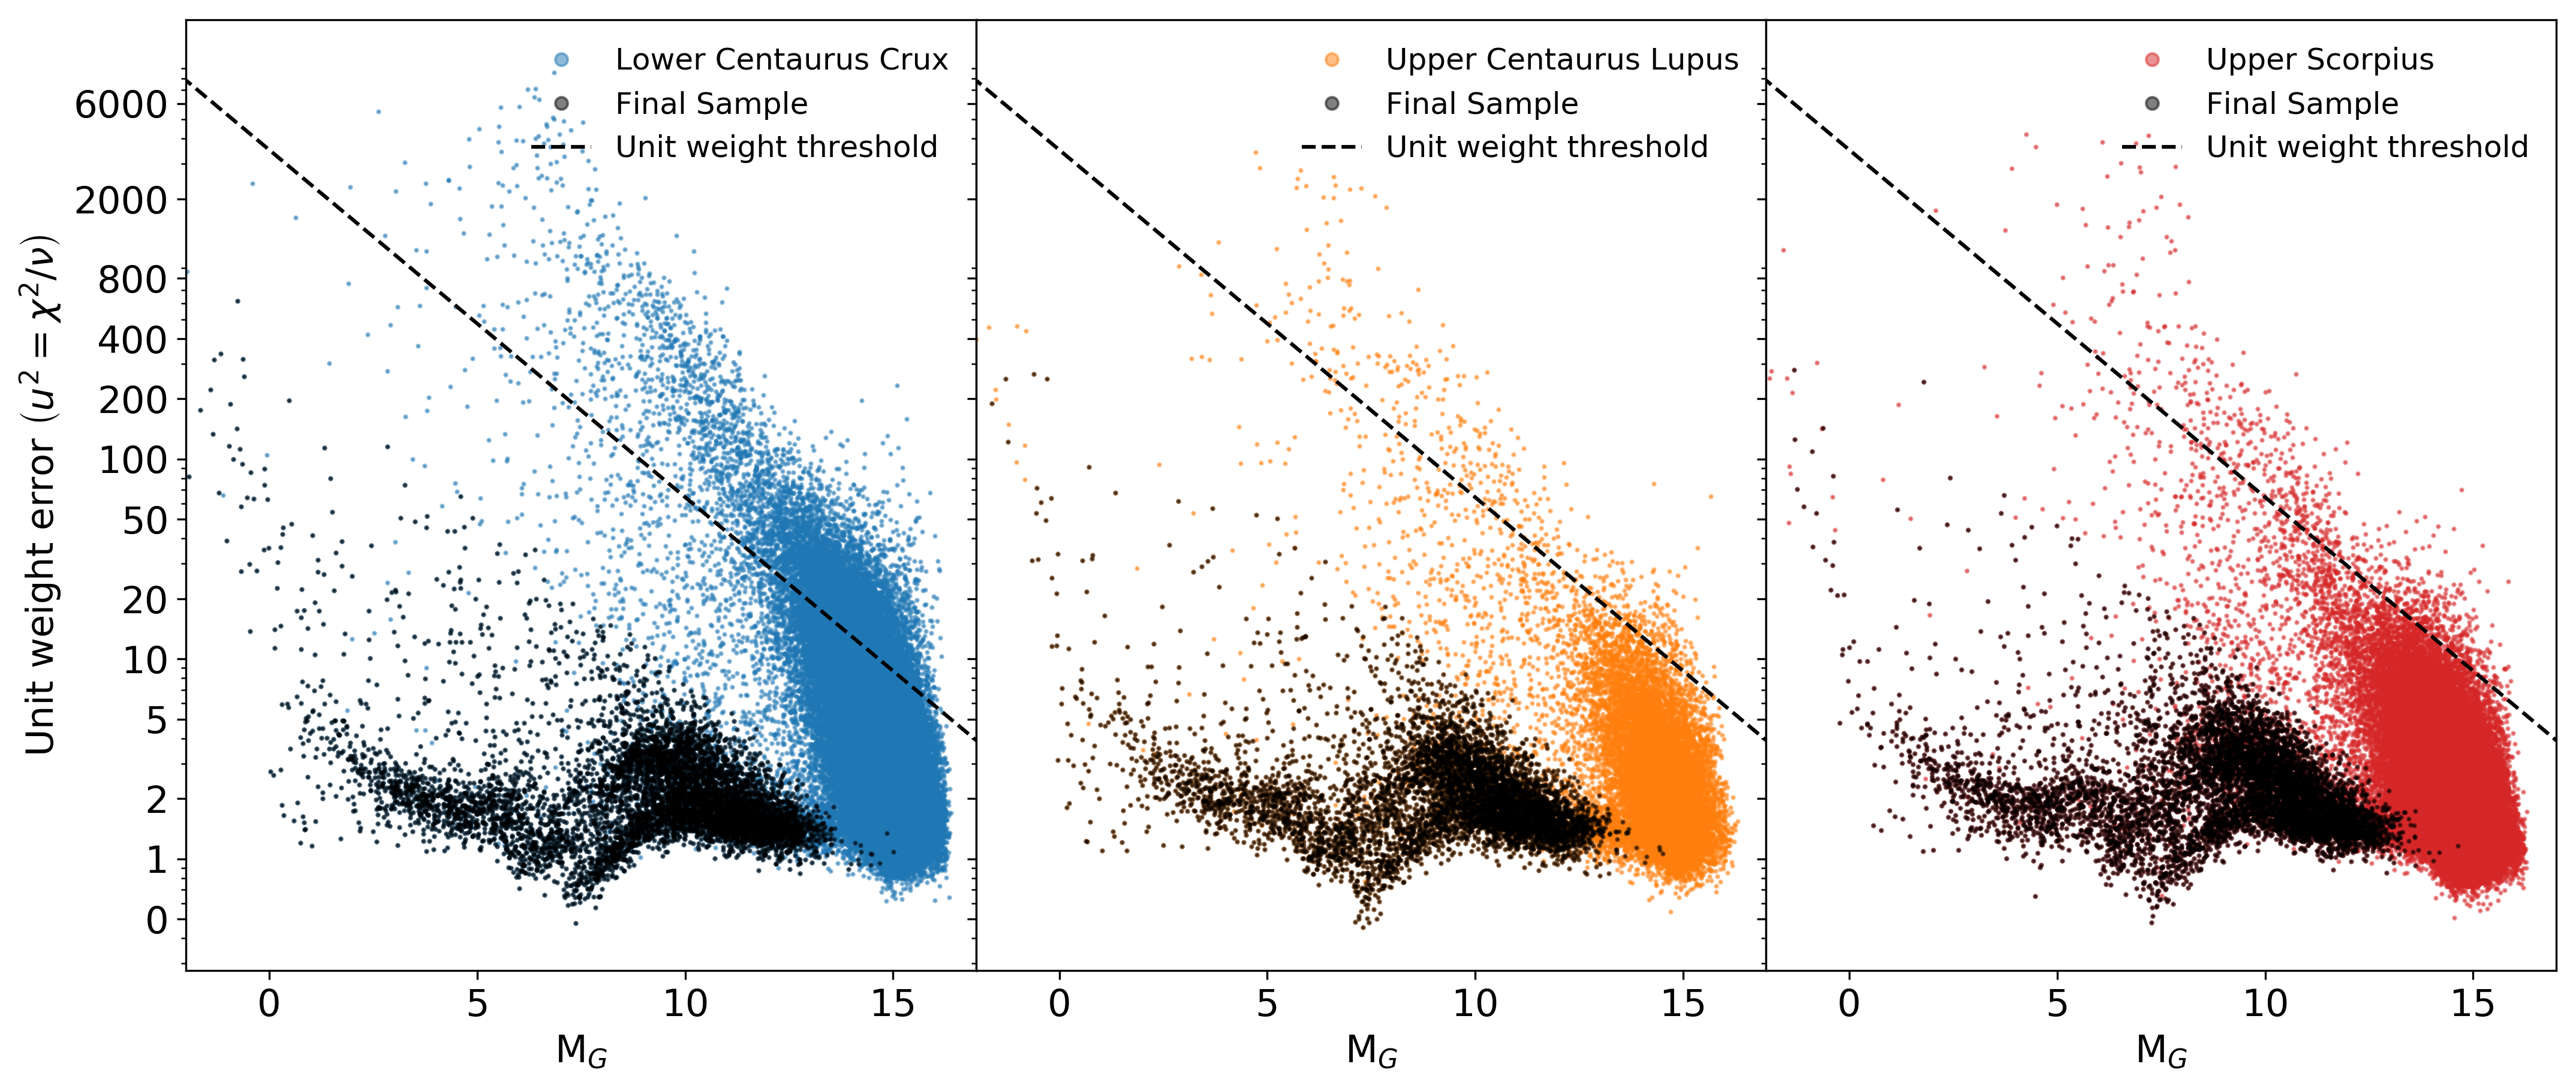
\includegraphics[width = 16cm, height = 7.5cm]{./Graficos/Capitulo_3/7_DR2_LightCurves/Lindegren_Selection.png}} 
% \caption{\scriptsize{Unit weight error threshold as proposed by \cauthor{2016ApJS..222....8D} \citeyear{2016ApJS..222....8D} to obtain photometric and astrometric cleaned data. The black line represents the threshold defined in \autoref{eq:WeightError}. \textit{Left}: LCC unit weight error as a function of magnitude in the $\textnormal{G}$-band. The blue dots represents the original sample as shown in \autoref{fig:NewData_DR2}-left panel, while the black dots correspond to the filtered by unit weight error and flux excess ratio. \textit{Center}: UCL unit weight error as a function of magnitude in the $\textnormal{G}$-band. The orange dots represents the original sample as shown in \autoref{fig:NewData_DR2}-center panel, while the black dots correspond to the filtered by unit weight error and flux excess ratio. \textit{Right}: US unit weight error as a function of magnitude in the $\textnormal{G}$-band. The red dots represents the original sample as shown in \autoref{fig:NewData_DR2}-right panel, while the black dots correspond to the filtered by unit weight error and flux excess ratio.}}
% \label{fig:LindegrenSelection}
% \end{figure}
% 
% \begin{figure}[!ht]
% \centering
%   \subfloat{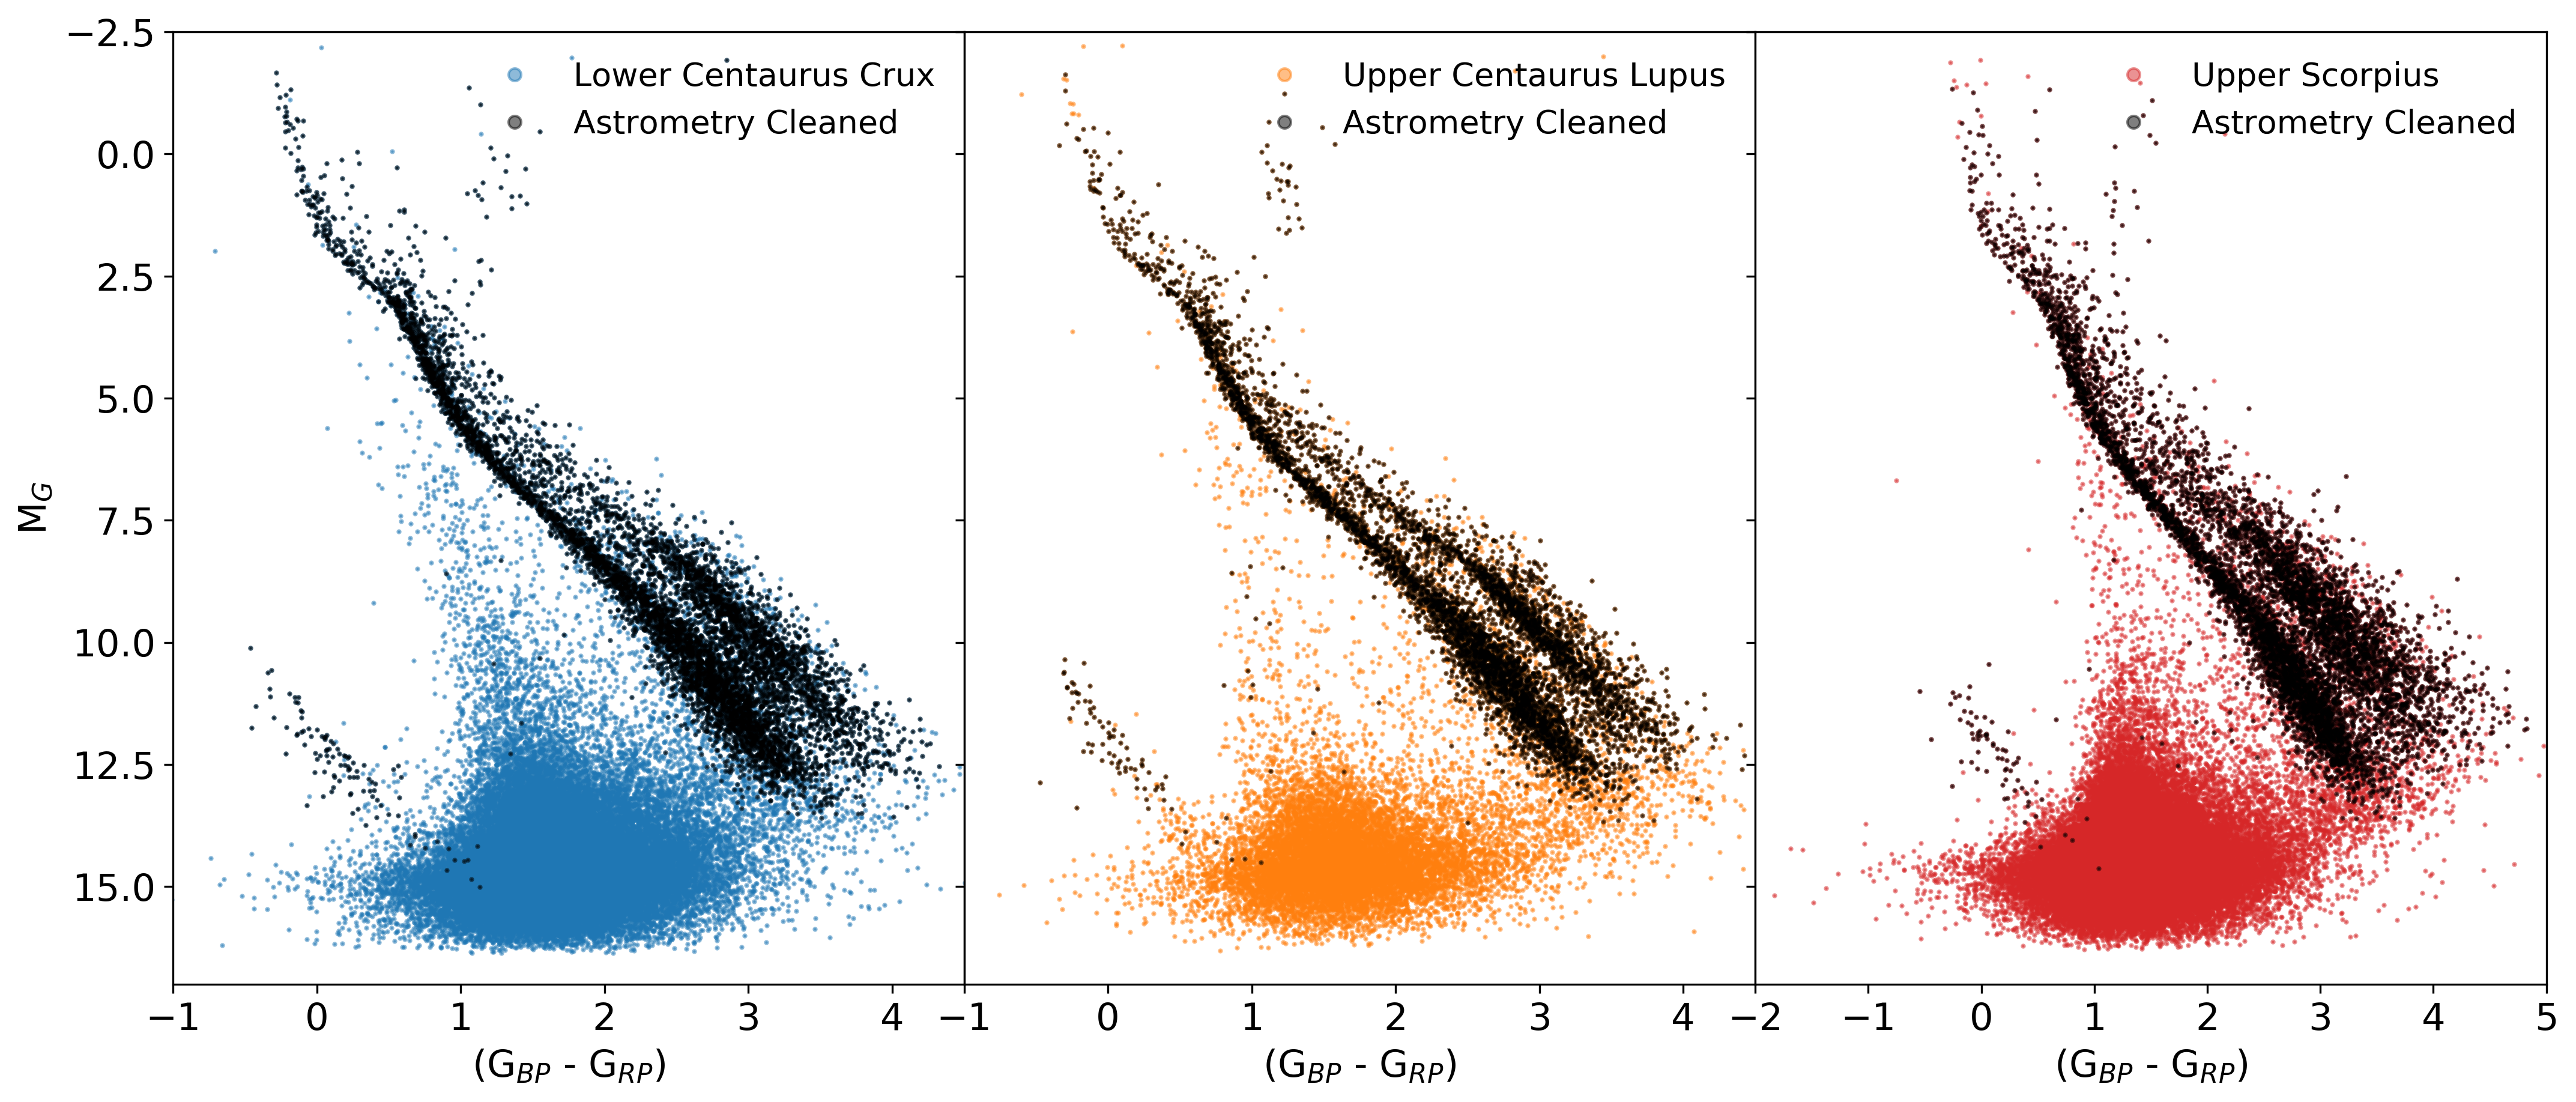
\includegraphics[width = 15.5cm, height = 7.5cm]{./Graficos/Capitulo_3/7_DR2_LightCurves/CMD_Cleaned_MG.png}} 
% \caption{\scriptsize{Color-magnitude diagram using \textit{Gaia}-DR2 data for each subgroup in ScoCen filtered by unit weight error and flux excess ratio. \textit{Left}: LCC absolute magnitude in the $\textnormal{G}$-band as a function of color-index $\textnormal{G}_\textnormal{BP} - \textnormal{G}_\textnormal{RP}$. \textit{Center}: UCL absolute magnitude in the $\textnormal{G}$-band as a function of color-index $\textnormal{G}_\textnormal{BP} - \textnormal{G}_\textnormal{RP}$. \textit{Right}: US absolute magnitude in the $\textnormal{G}$-band as a function of color-index $\textnormal{G}_\textnormal{BP} - \textnormal{G}_\textnormal{RP}$. The color dots show the original sample as presented in \autoref{fig:NewData_DR2}, while the black dots correspond to the final sample after correcting the flux excess ratio and unit weight error as shown in \autoref{fig:LindegrenSelection}.}}
% \label{fig:FinalSample_DR2}
% \end{figure}

In the original data retrieved using \textit{Gaia} DR2 we obtained $15\,074$, $9\,658$, and $14\,580$ for LCC, UCL, and US respectively. After performing the cleaning process to correct for spurious parallaxes and colors, we end up with a sample of $7\,268$, $6\,244$, and $7\,436$ for LCC, UCL, and US respectively (see \autoref{fig:LindegrenSelection}). In comparison to \textit{Gaia} DR1 an increase in sources is noticeable, specially for $\textnormal{M}_\textnormal{G} > 7$ (see \autoref{fig:Isochrones_4}). Also, there is a clear division between the pre-main sequence and the main-sequence population in each one of the subgroups, exposing how powerful \textit{Gaia} DR2 can be. Exactly the same selection process applied to the \textit{Gaia} DR1 was done to this new sample in order to select the stars and lately cross-match them with the \textit{SuperWASP} database and obtain the light curves. In \autoref{fig:DR2_Comparison}, the absolute magnitude in band-G as a function of color is presented for each subgroup. The two lines correspond to $5$Myr and $60$Myr isochrones, where the youngest isochrone has been computed using the mean extinction values calculated in \autoref{fig:SCOCEN_Extinction}. The final sample corresponds to stars between both isochrones. As can be observed in \autoref{fig:DR2_Comparison} and \autoref{fig:DR2_Selection}, the isochrones models have a lower limit in absolute magnitude around $\textnormal{M}_\textnormal{G} \backsimeq 10$, at least for the $5$Myr isochrone. Thus, we decided to cut in this values, although an interpolation of the isochrones is possible if one wants to go down to lower values in absolute magnitude which means obtaining more low-mass stars. This is clearly seen in \autoref{fig:DR2_Tracks} where different stellar tracks are shown for selected stars to check how low in stellar mass we can go with the new data set. Using \textit{Gaia} DR1 we had a limit close to $\sim0.9\textnormal{M}_\odot$ (see \autoref{fig:Stellar_Tracks_3}) however, with \textit{Gaia} DR2   this limit has gone down to $\sim0.1\textnormal{M}_\odot$ which is indeed the limit of the stellar track models. It is worthy to note that if we do not perform any cut in absolute magnitude, we can go down to $\textnormal{M}_\textnormal{G}\sim14$, which basically means that if we compare \autoref{fig:DR2_Comparison} and \autoref{fig:DR2_Selection} we can include a huge sample of quite low-mass stars which are out of our final sample. This could be addressed in a future work to compare how much the pre-selection in \textit{Gaia} DR2 and the cross-matching with the \textit{SuperWASP} changes. Having said that, we can guarantee that the final sample has enough low-mass stars in the ScoCen OB association to be studied in more detail as these are the type of stars likely to show exoplanetary ring transits. Additionally, to verify that the final sample corresponds to the original sky selection after all the cleaning- and -selection process, the sky distribution is shown in \autoref{fig:DR2_Projection} for each one of the subgroups in a Hammer-Aitoff projection using Galactic coordinates.     

\begin{figure}[!ht]
\centering
  \subfloat{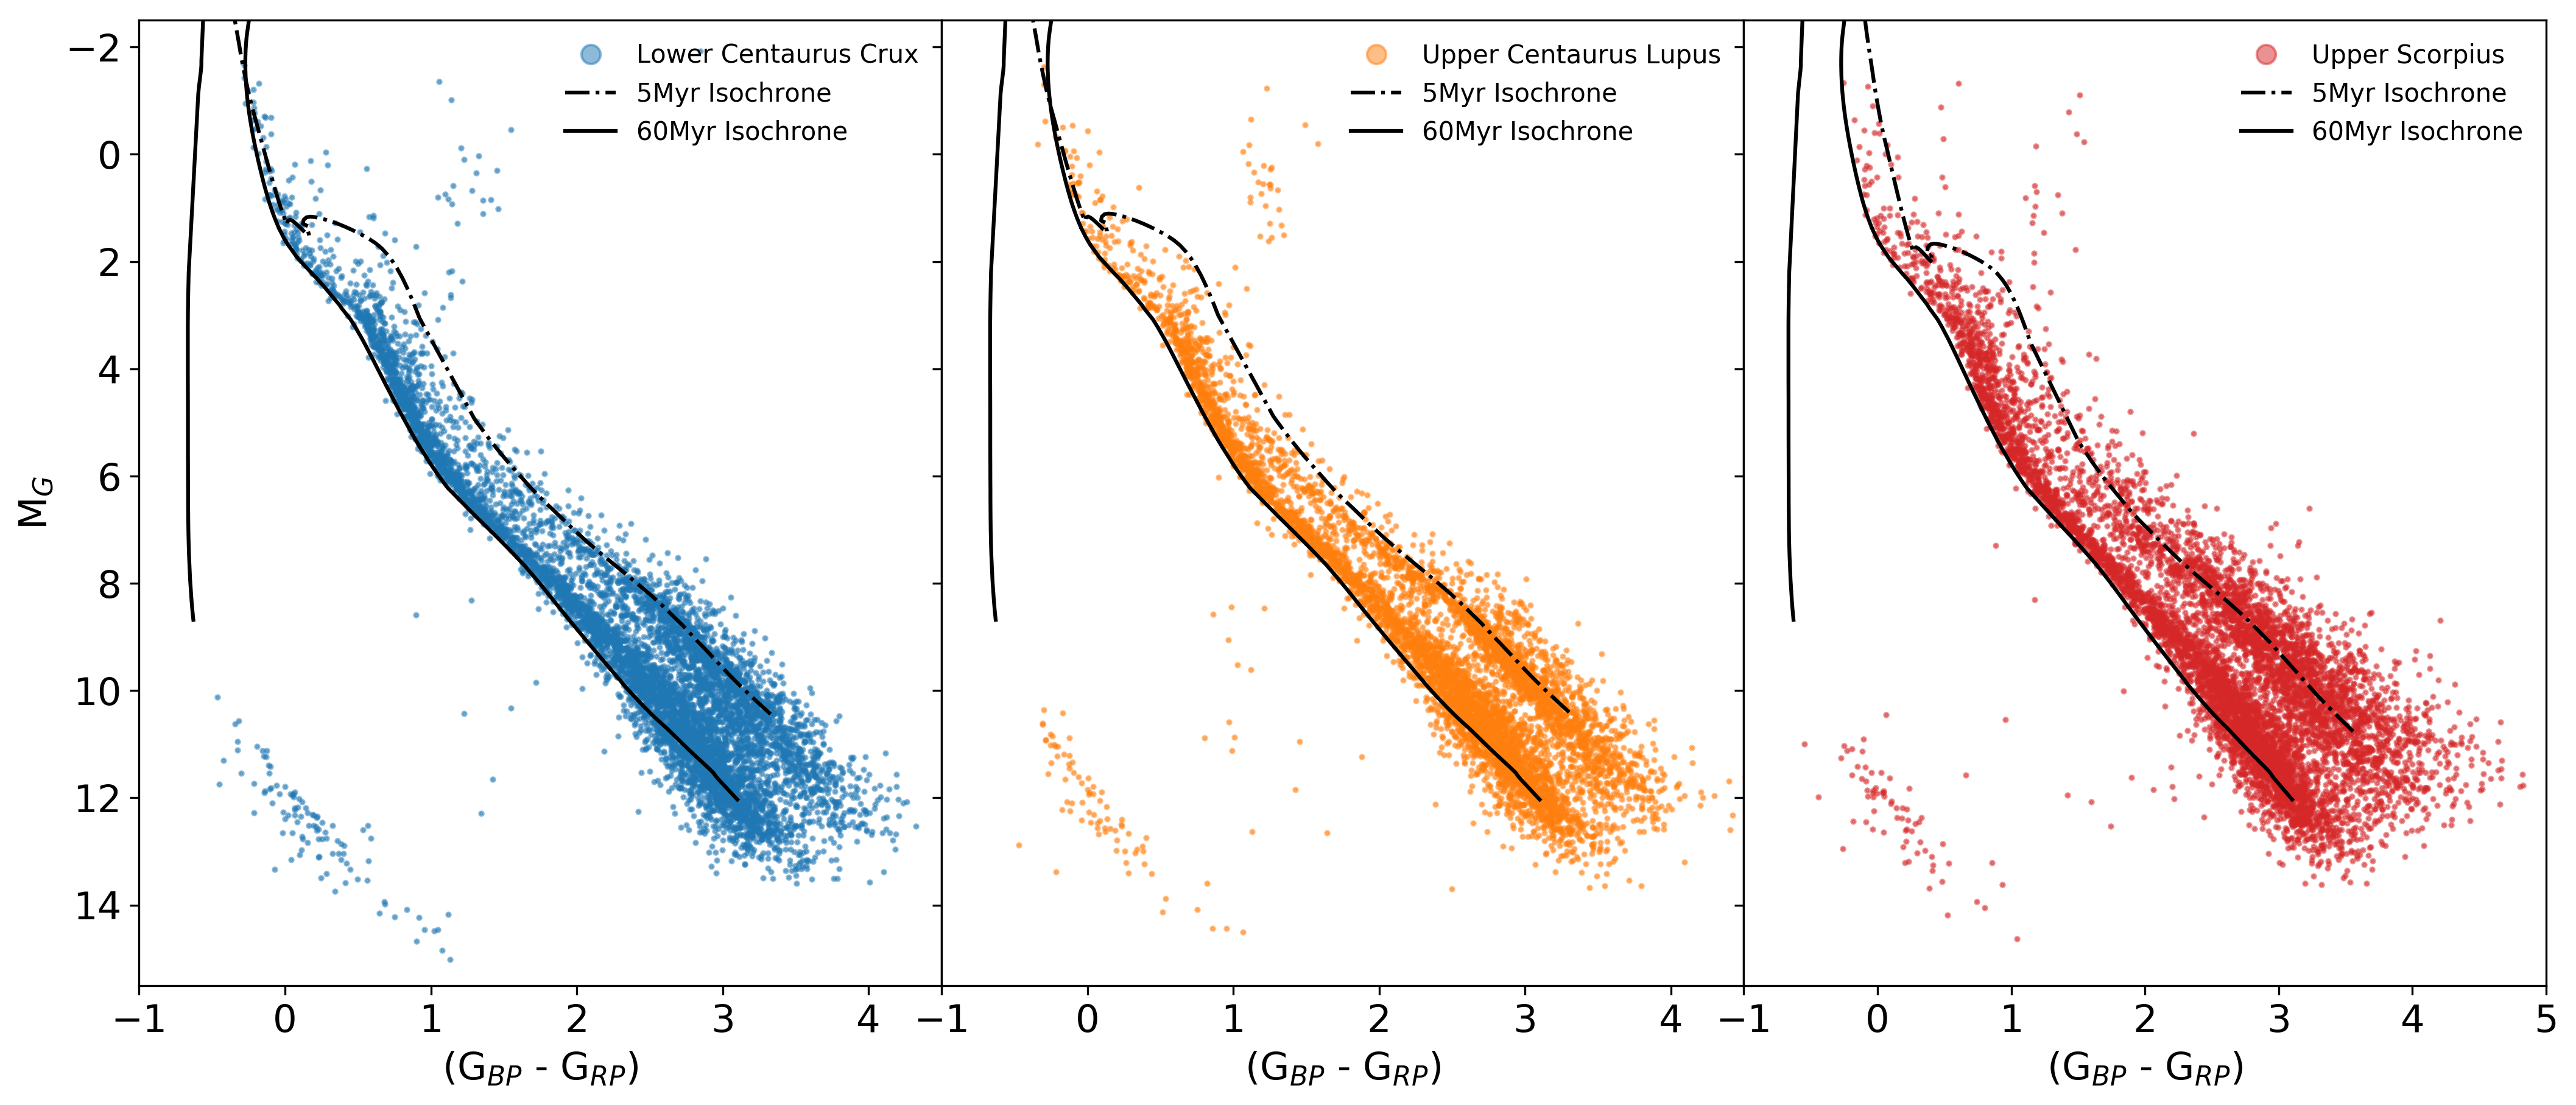
\includegraphics[width = 16cm, height = 7.5cm]{./Graficos/Capitulo_3/7_DR2_LightCurves/CMD_Clean_Iscohrones.png}} 
\caption{\scriptsize{Color-magnitude diagram using the filtered out sample for each subgroup in ScoCen as presented in \autoref{fig:FinalSample_DR2}. \textit{\textbf{Left}}: LCC absolute magnitude in the $\textnormal{G}$-band as a function of color-index $\textnormal{G}_\textnormal{BP} - \textnormal{G}_\textnormal{RP}$. \textit{\textbf{Center}}: UCL absolute magnitude in the $\textnormal{G}$-band as a function of color-index $\textnormal{G}_\textnormal{BP} - \textnormal{G}_\textnormal{RP}$. \textit{\textbf{Right}}: US absolute magnitude in the $\textnormal{G}$-band as a function of color-index $\textnormal{G}_\textnormal{BP} - \textnormal{G}_\textnormal{RP}$. The color dots represent the cleaned data, while the lines show two isochrones of $5 \textnormal{Myr}$, and $60 \textnormal{Myr}$, respectively, computed using $\textnormal{A}_\textnormal{v} = 0.23$, $\textnormal{A}_\textnormal{v} = 0.17$, and $\textnormal{A}_\textnormal{v} = 0.76$, for each subgroup. The new isochrones are computed with updated bandpasses corresponding to the \textit{Gaia}-DR2 using \textit{MIST}-package.}}
\label{fig:DR2_Comparison}
\end{figure}

\begin{figure}[!ht]
\centering
  \subfloat{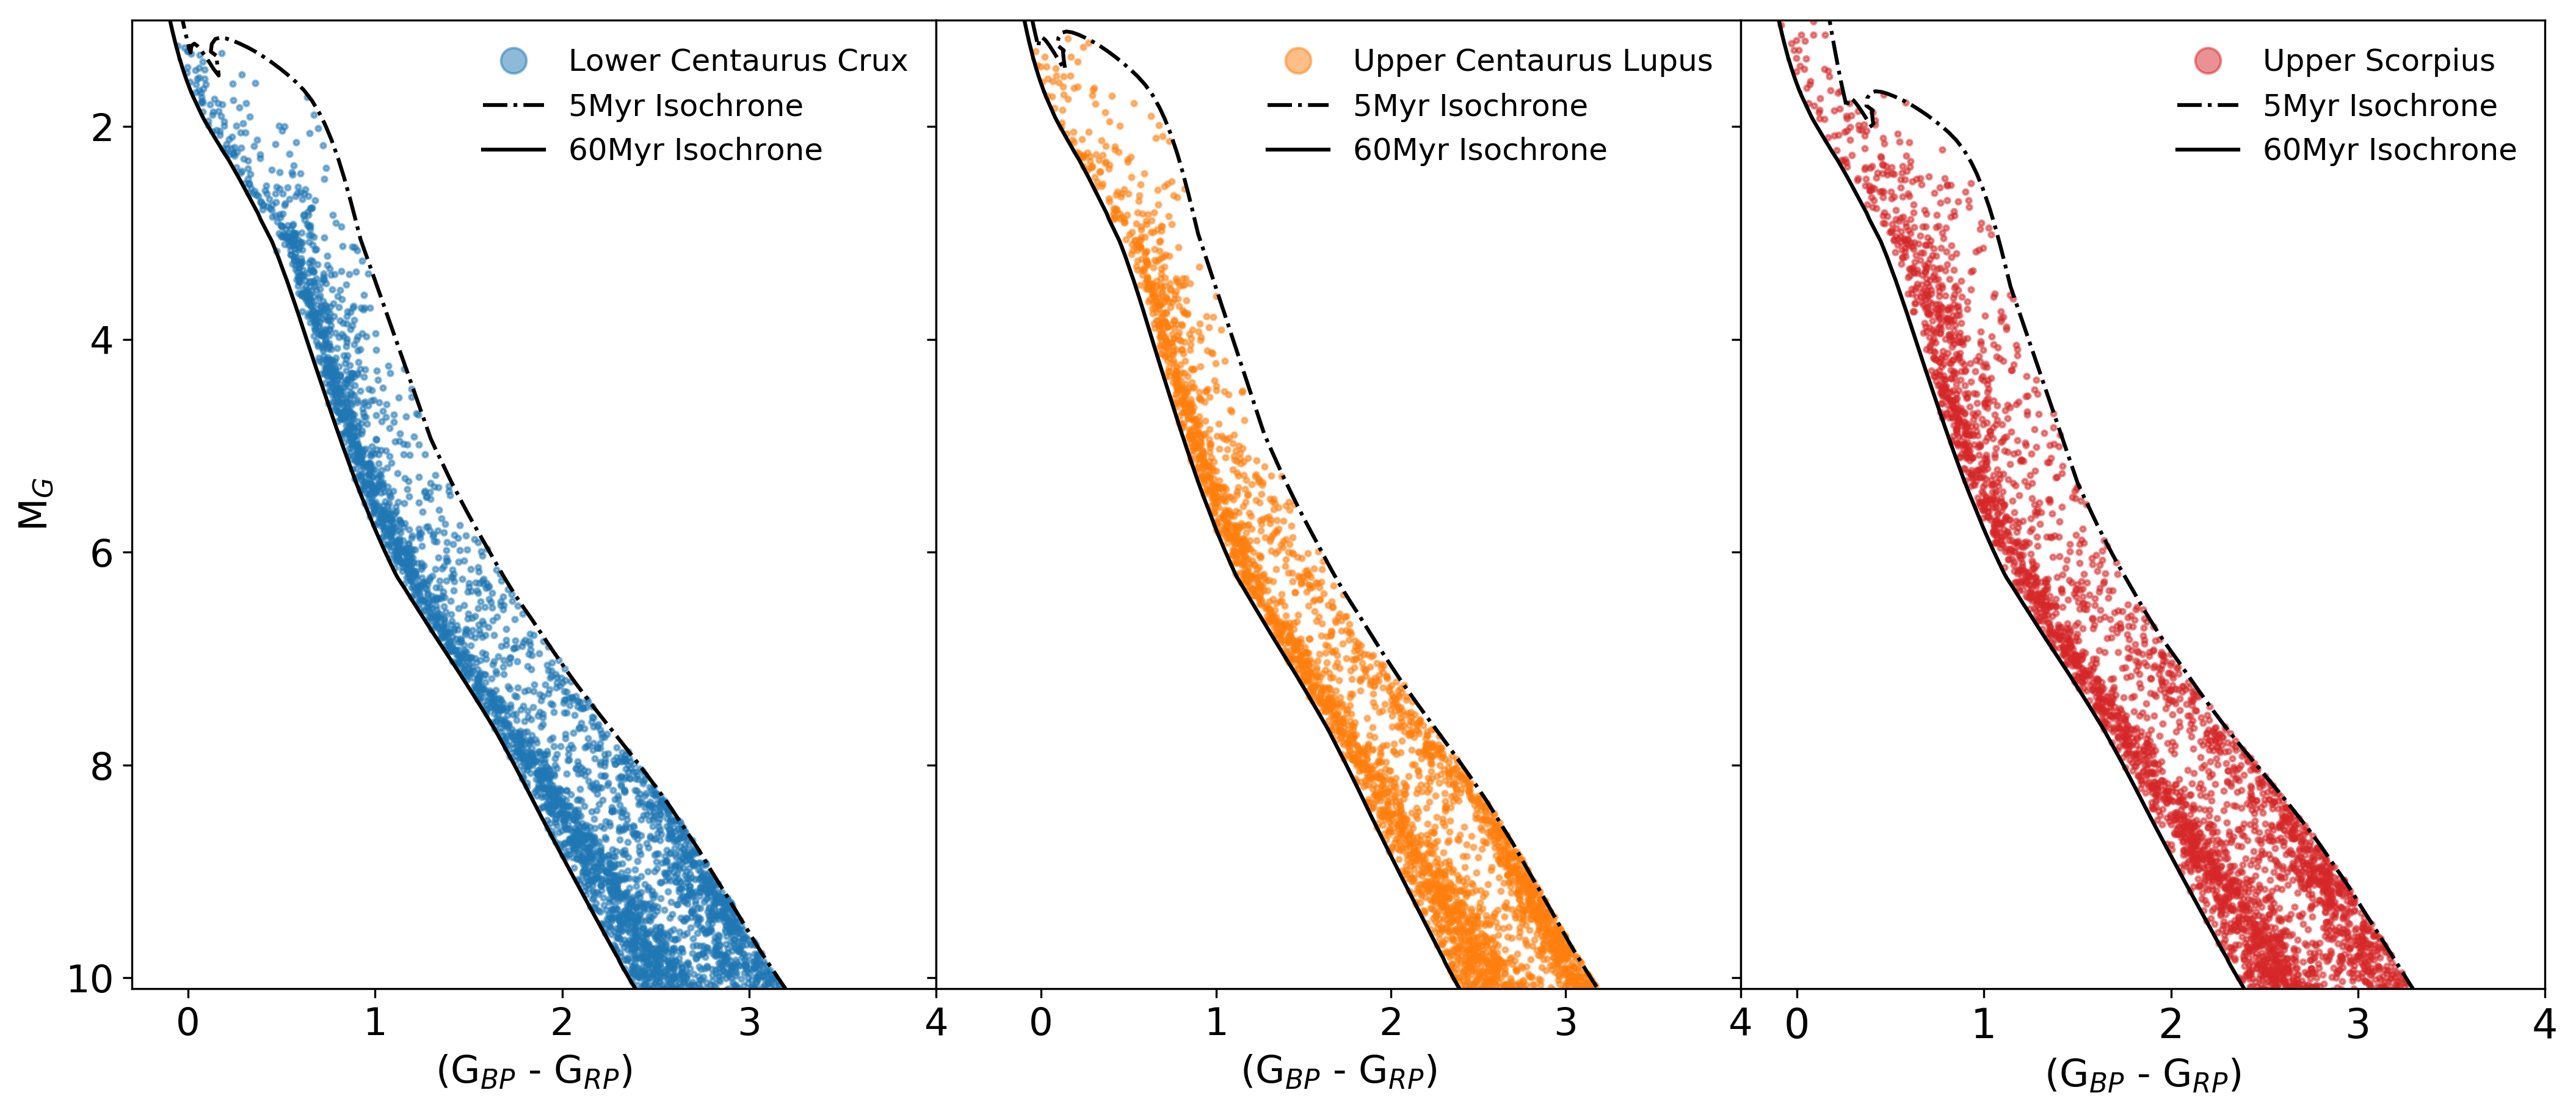
\includegraphics[width = 16cm, height = 7.5cm]{./Graficos/Capitulo_3/7_DR2_LightCurves/CMD_Clean_FinalSelection.png}} 
\caption{\scriptsize{Color-magnitude diagrams for each subgroup in ScoCen using the filtered out sample between two different isochrones applying the extinction value proposed by \cauthor{1989A&A...216...44D} (\citeyear{1989A&A...216...44D}). \textit{\textbf{Left}}: LCC stars after cuts are shown in blue. The black lines correspond to different isochrones. \textit{\textbf{Center}}: UCL stars after cuts are shown in orange. The black lines correspond to different isochrones. \textit{\textbf{Right}}: US stars after cuts are shown in red. The black lines correspond to different isochrones. Only the $5 \textnormal{Myr}$ to $60 \textnormal{Myr}$ isochrones were used to restrict the sample of stars to be inside this particular region. Following this, stars inside the region are quite likely to belong to the cluster and be in an stellar age range suitable for our study. In this case, the extinction values for LCC, UCL, and US correspond to $\textnormal{A}_\textnormal{v} = 0.23$, $\textnormal{A}_\textnormal{v} = 0.17$, and $\textnormal{A}_\textnormal{v} = 0.76$, respectively.}}
\label{fig:DR2_Selection}
\end{figure}

\begin{figure}[!ht]
\centering
  \subfloat{\includegraphics[width = 16cm, height = 7.5cm]{./Graficos/Capitulo_3/7_DR2_LightCurves/CMD_Cleaned_FinalSelection_Tracks.png}} 
\caption{\scriptsize{Color-magnitude diagrams for each subgroup in ScoCen using the filtered out sample, along with stellar tracks using the extinction value proposed by \cauthor{1989A&A...216...44D} (\citeyear{1989A&A...216...44D}). \textit{\textbf{Left}}: LCC stars after cuts are shown in blue. The black lines correspond to different stellar tracks. \textit{\textbf{Center}}: UCL stars after cuts are shown in orange. The black lines correspond to different stellar tracks. \textit{\textbf{Right}}: US stars after cuts are shown in red. The black lines correspond to different stellar tracks. In general for each subgroup, a stellar mass range of $0.1 \textnormal{M}_\odot < \textnormal{M} < 2.4 \textnormal{M}_\odot$ was used to compute the stellar tracks using the \textit{MIST}-package (\cauthor{2016ApJS..222....8D} \citeyear{2016ApJS..222....8D}; \cauthor{2016ApJ...823..102C} \citeyear{2016ApJ...823..102C}). In this case, the extinction values for LCC, UCL, and US correspond to $\textnormal{A}_\textnormal{v} = 0.23$, $\textnormal{A}_\textnormal{v} = 0.17$, and $\textnormal{A}_\textnormal{v} = 0.76$, respectively.}}
\label{fig:DR2_Tracks}
\end{figure}

\begin{figure}[!ht]
\centering
  \subfloat{\includegraphics[width = 16cm, height = 8cm]{./Graficos/Capitulo_3/7_DR2_LightCurves/Sco_Cen_FinalSample_Projection.png}} 
\caption{\scriptsize{ScoCen subgroups position in galactic coordinates. Each subgroup LCC (blue), UCL (orange) and US (red), contains the final sample of stars after cleaning \textit{Gaia} DR2 data shown in galactic longitude and galactic latitude. The region covers $\sim 90$-degrees in longitude and $\sim 50$-degrees in latitude.}}
\label{fig:DR2_Projection}
\end{figure}

The final sample and the cross-matching process is addressed in \autoref{sec:LightCurvesSco} and the special case of J1407.

%============================================================================================================================================================

\section{ScoCen Light Curves}\label{sec:LightCurvesSco}

In the last section, we explained the selection process to obtain the final sample of stars in each subgroup of ScoCen using \textit{Gaia} DR2 data. Now, as we want to obtain the light curves available for these stars in the \textit{SuperWASP} database, the next step is to cross-match each object using their coordinates in right ascension and declination. The \href{https://exoplanetarchive.ipac.caltech.edu/cgi-bin/TblSearch/nph-tblSearchInit?app=ExoTbls&config=superwasptimeseries}{SuperWASP-Interface} allows the user to search for an object's light curve using its coordinates including constraints as the start and end of the light curve, the number of data points used in the statistical calculation, the number of points in the actual light curve, the WASP-magnitude, among others. In our particular case, we decided to pass each set of stars in each of the ScoCen subgroups as a list and search for any object within a radius of $0.1~\textnormal{arcsec}$ to ensure that the selected stars correspond to the one measured in \textit{Gaia} DR2. Along with this, the only extra constraint we set was the number of points in the light curve to be greater than $100$ because lots of stars have poor measurements and it is not worthy to retrieve them. Following this steps, we get a final sample of $177$, $1\,053$, and $1\,253$ light curves for LCC, UCL, and US out of the $7\,268$, $6\,244$, and $7\,436$ original sample after all the cuts were applied. It is striking the small number of light curves retrieved for LCC having in mind that for the three subgroups the number of stars is very similar. However, if we observe \autoref{fig:SWASP_DR1_Flux} in \autoref{sec:SWASPdata}, LCC lies close to the mid-plane of the Milky Way where the \textit{SuperWASP} survey is incomplete. In the same way, US happens to have a large number of stars retrieved due to the fact that this subgroup lies in a portion of the night sky which was widely surveyed. The light curves are generated automatically from the data files retrieved for each one of the targets using corrected values of the apparent magnitude as a function the Julian Day.\\

Having said that, we proceed to inspect the light curves possibly showing up features as those reported by \cauthor{2012AJ....143...72M} (\citeyear{2012AJ....143...72M}) for J1407. Our selection criteria retrieve this object in the UCL-subgroup when using the unit weight error cleaning $u$. However, if we apply the $u^2$ criterion then this object is left out of the sample. In spite of that, the method gives us hope in our blind-search for exoplanetary rings. The light curve without averaging the data per night is shown in \autoref{fig:J1407WASPLC}. The dataset corresponds to three different years of observation where the second-year exhibits a remarkable dip. This is the type of features we are interested in because it is the closest report in literature to be a ringed system, thus, we took this as a canonical example for comparison with all the different light curves obtained through the cross-match. Initially, the main scientific aim was to retrieve the light curves and pre-select possible candidates to fit different disks models. However, we decided to just provide a list of interesting light curves showing features as those in J1407 or simply any weird/unexpected variation as inspected by eye. The amount of data is quite large which makes the main goal of the project quite ambitious to achieve in a short time period. Thus, we proposed a final sample of candidates which could be followed up with new observations to complete the light curves that must be averaged per night, so in future works, the final analysis and disk-model fitting can be performed on this sample in order to rule out candidates. The final list of candidates is shown in \autoref{tab:Candidates_Final} where each source has its corresponding \textit{Gaia} DR2 and \textit{SuperWASP} IDs, and right ascension and declination, and the respective error as provided by \textit{Gaia} DR2 data.\\

\begin{figure}[!ht]
\centering
  \subfloat{\includegraphics[width = 15cm, height = 7cm]{./Graficos/Capitulo_3/7_DR2_LightCurves/J1407.png}} 
\caption{\scriptsize{1SWASP J$140747.93-394542.6$ (J$1407$) light curve. The figure shows the corrected magnitude as a function of HJD (days) for three different years of observation. A huge dip can be observed during the second-year which is assumed to be produce by a massive system of circumplanetary rings as reported in \cauthor{2012AJ....143...72M} (\citeyear{2012AJ....143...72M}).}}
\label{fig:J1407WASPLC}
\end{figure}

%Candidates 
\begin{table}[]
\centering
\caption{\textit{SuperWASP} candidates cross-matched with \textit{Gaia} DR2.}
\label{tab:Candidates_Final}
\scalebox{0.8}{
\begin{tabular}{llllll}
\hline \textit{Gaia} DR2 ID         & \textit{SuperWASP} ID               & RA {[}deg{]}        & RA\_ERR {[}deg{]} & DEC {[}deg{]}       & DEC\_ERR {[}deg{]}  \\ \hline \hline
 5375292381453195264 & 1SWASP J112917.08-461225.0 & 172.3215  & 0.0499  & -46.2071  &  0.0426  \\
 6107318842082097152 & 1SWASP J134703.99-460848.3 & 206.7665  & 0.0939  & -46.1468  &  0.0617  \\
 6116150703591896064 & 1SWASP J141849.15-394422.5 & 214.7045  & 0.0989  & -39.7397  &  0.1185  \\
 6103779101835413504 & 1SWASP J142352.01-411304.8 & 215.9665  & 0.0533  & -41.2182  &  0.0437  \\
 6098745709402994688 & 1SWASP J143906.15-451537.0 & 219.7756  & 0.0302  & -45.2604  &  0.0378  \\
 6229363700751409152 & 1SWASP J145223.73-244648.9 & 223.0987  & 0.0433  & -24.7804  &  0.0288  \\
 6100760014705034240 & 1SWASP J145302.55-425247.5 & 223.2606  & 0.0387  & -42.8799  &  0.0377  \\
 6198287589442119680 & 1SWASP J145822.27-382555.3 & 224.5929  & 0.0443  & -38.4319  &  0.0454  \\
 6206539802163648512 & 1SWASP J152836.36-334750.3 & 232.1515  & 0.1352  & -33.7974  &  0.0407  \\
 6039361223829141504 & 1SWASP J155606.62-321225.8 & 239.0274  & 0.0189  & -32.2073  &  0.0097  \\
 6042706591035865088 & 1SWASP J160158.04-283057.4 & 240.4919  & 0.0356  & -28.5161  &  0.0159  \\
 6043692028329650176 & 1SWASP J160728.47-254832.8 & 241.8686  & 0.0538  & -25.8091  &  0.0219  \\
 6041822716821447680 & 1SWASP J160826.31-282549.3 & 242.1095  & 0.0422  & -28.4305  &  0.0173  \\
 6043701064940930048 & 1SWASP J160833.29-254010.6 & 242.1386  & 0.0539  & -25.6696  &  0.0253  \\
 6038079708665729024 & 1SWASP J162339.37-294405.6 & 245.9139  & 0.0499  & -29.7349  &  0.0339  \\
 6045393041544132608 & 1SWASP J162452.74-265517.0 & 246.2199  & 0.0593  & -26.9213  &  0.0334  \\ \hline 
\end{tabular}
}
\end{table}

Some light curves show double measurements in different years caused by an object being detected in different cameras and flux not being matched properly. For this reason, we decided to draw the apparent magnitude corrected by \autoref{eq:Mag_Swasp} as a function of HJD as given by \autoref{eq:HJD_Swasp} which helps us to avoid this type of spurious features. However, it is worth noticing that even after correcting the flux (i.e. apparent magnitude) this kind of features are still present for a couple of sources in which we cannot attribute it as a result of bad matching or real measurements. This can be observed in \autoref{fig:SWASP_LightCurve_1} for the second year of observations where the light curve has already been corrected. In \autoref{fig:SWASP_LightCurve_Spurious} and \autoref{fig:SWASP_LightCurve_2}, we present two candidates in order to illustrate how any other light curve looks like in our final sample. It is clear that these light curves do not exhibit dramatic dips as compared to J1407. However, interesting features are present which motivate future work and observations. \autoref{fig:SWASP_LightCurve_2} on the other hand gives the impression of a regular variable star instead of a ringed system around. We decided to keep also this type of light curves because we already have coordinates, parallaxes, and proper motions for all these stars thanks to \textit{Gaia} DR2 which may lead to possible new discoveries.  

\begin{figure}[!ht]
\centering
  \subfloat{\includegraphics[width = 15cm, height = 7cm]{./Graficos/Capitulo_3/7_DR2_LightCurves/1SWASPJ135747.png}} 
\caption{\scriptsize{1SWASP J$135747.65-321915.5$ light curve. The figure shows the corrected magnitude as a function of HJD (days) for three different years of observation. During the second-year there is a double feature likely to be produced by bad match between different fluxes in different cameras of the \textit{SuperWASP} survey.}}
\label{fig:SWASP_LightCurve_1}
\end{figure}

\begin{figure}[!ht]
\centering
  \subfloat{\includegraphics[width = 15cm, height = 7cm]{./Graficos/Capitulo_3/7_DR2_LightCurves/1SWASP_J162339.png}} 
\caption{\scriptsize{1SWASP J$162339.37-294405.6$ light curve. The figure shows the corrected magnitude as a function of HJD (days) for three different years of observation. During the second-year there is a feature that reminds the observations of J1407 in $2012$.}}
\label{fig:SWASP_LightCurve_Spurious}
\end{figure}

\begin{figure}[!ht]
\centering
  \subfloat{\includegraphics[width = 15cm, height = 7cm]{./Graficos/Capitulo_3/7_DR2_LightCurves/1SWASP_J145822.png}} 
\caption{\scriptsize{1SWASP J$145822.27-382555.3$ light curve. The figure shows the corrected magnitude as a function of HJD (days) for three different years of observation. The light curve presents a variations that gives the sensation of a sinusoidal curve. Day average and model fitting are needed to give a final verdict.}}
\label{fig:SWASP_LightCurve_2}
\end{figure}

%\subsection{J1407 light curve}\label{subsec:LightCurvesSco_1}

%============================================================================================================================================================

\section{ScoCen Pre-Main Sequence Population}
%\cauthor{} \citeyear{}

In different works as those by (\cauthor{1999AJ....117..354D} \citeyear{1999AJ....117..354D}; \cauthor{2018MNRAS.tmp..210W} \citeyear{2018MNRAS.tmp..210W}) kinematic analysis from proper motions and radial velocities has been essential to study OB associations as ScoCen in order to separate members from the foreground and background stellar population. Spectroscopic and photometric surveys usually lack low-mass pre-main sequence stars creating a bias towards more massive members. In 2017 \cauthor{Zari17} (\citeyear{Zari17}) used \textit{Gaia} DR1 data to isolate the pre-main sequence population in the Orion region using the apparent magnitude versus color and combining also \textit{2MASS} photometry. On the other hand \cauthor{Skrutskie06} (\citeyear{Skrutskie06}) also addressed the same problem but using \textit{Gaia} DR2 data and constructing the Hertzsprung-Russell in which the pre-main sequence population is more precisely isolated. In our case, we decided to apply the same method but to the ScoCen region because this provides an easy way to pre-select member of the association and search for probably hidden features.\\

In the first place, we extended the original three boxes which limit the \textit{Scorpius-Lupus-Centaurus-Crux} area on the sky \cauthor{Blaauw46} (\citeyear{Blaauw46}). The new limits contain the original three boxes and correspond to all stars with galactic coordinates $285^\circ\leq\ell\leq360^\circ$ and $-10^\circ\leq b\leq+32^\circ$. This is shown in the right panel of \autoref{fig:ScoOB_premain} in which the color map stands for the logarithmic number of stars in hexagon bins. Additionally, the new range of parallax was set to lie between $5$ and $12$ mas to cover a wider volume in space. No cuts in right ascension and declination proper motions or total proper motion were used just to leave the sample as free as possible of constraints known in the literature due to the fact that if the method of pre-selecting the pre-main sequence is powerful enough, then the overall features of the OB association will pop up naturally. Sources with spurious parallaxes and bad photometry were cleaned following the same method explained in \autoref{sec:CleaningProcess} as proposed in \cauthor{2018arXiv180409366L} (\citeyear{2018arXiv180409366L}). The first sample contains $134\,587$ source, however, after the selection process our sample is made up of $120\,911$ sources represented as blue dots in the left of \autoref{fig:ScoOB_premain} which corresponds to the Hertzsprung-Russell diagram. It is worth noticing that the pre-main sequence and main-sequence populations are well separated for $(G_\mathrm{BP}-G_\mathrm{RP})>1$, where at $(G_\mathrm{BP}-G_\mathrm{RP})>2$ the separation is well above the $0.75$ magnitude expected from a population of equal mass binaries. Thus, we proceeded to select the young population in our sample using an interactive selection method which allows us to draw a polygon around the region of study and then retrieve the information associated to sources inside the polygon. The polygon and notebooks are available at Zenodo, \href{https://zenodo.org/record/1286576#.Wx6NAmMzaV4}{doi:10.5281/zenodo.1286576}.\\ 

\begin{figure}[!ht]
\centering
  \subfloat{\includegraphics[width = 16cm, height = 8.5cm]{./Graficos/Capitulo_3/ScoCen_Coordinates.png}} 
\caption{\scriptsize{Color-magnitude diagram of the ScoCen region. The orange dots represent the young population selected (pre-main sequence stars) while the blue dots represents the whole sample after the cleaning process. \textit{\textbf{Bottom right:}} Sky distribution of the young stellar population. The classical boundaries of the three subgroups of ScoCen (from left to right, \textit{Upper Scorpius}, \textit{Upper Centaurus-Lupus}, and \textit{Lower Centaurus-Crux}), as defined in \cauthor{1999AJ....117..354D} (\citeyear{1999AJ....117..354D}), are indicated. \textit{\textbf{Top right:}} Distance distribution (with distance calculated as $1/\varpi$) as a function of Galactic longitude.}}
\label{fig:ScoOB_premain}
\end{figure}

In general, in \autoref{fig:ScoOB_premain} a clear concentration of pre-main sequence stars is evident following the original three-boxes region, consistent with most of the selected sources being association members. The LCC and UCL subgroups show a clear concentration of stars but relatively sparse in comparison to US which shows a remarkable high-density concentration of the selected young population. The expanded search reveals a notorious over-density out of the US original box-limits associated with ScoCen ($b\sim5^\circ$ and $\ell\sim345^\circ$) at a mean distance of $\sim180\mathrm{pc}$ ($5$-$6$~mas) (see \autoref{fig:ScoOB_premain} top-right panel). This feature was previously noted by \cauthor{1999AJ....117..354D} (\citeyear{1999AJ....117..354D}) (see their Section 4.5 and Figure 9), and in \cauthor{2016MNRAS.461..794P} (\citeyear{2016MNRAS.461..794P}) using \textit{Gaia} DR1 data. However, our sample contains more sources exposing this region with better clarity allowing new works following the kinematics analysis to have a higher chance of finding new stars which could belong to the OB association much more easily. There is also a concentration of sources near $(\ell,b)=(290^\circ,-5^\circ)$ which corresponds to the well-known IC 2602 cluster lying at $\varpi = 6.74 \pm 0.25$~mas as reported by (\cauthor{vanLeeuwen17} \citeyear{vanLeeuwen17}). Thus, in overall, the resulting maps of the pre-main sequence population can be used to guide more detailed membership studies of OB associations, including a thorough re-assessment of the traditional association and subgroup boundaries. We anticipate a major revision in our knowledge of OB associations coupled with new insights into the triggering and propagation of star formation.\\

Summing up, it turns out to be quite useful to use \textit{Gaia} DR2 data in order to retrieve sources of a volume-limited sample in parallax and coordinates to lately build up the Hertzsprung-Russell diagram and select the young population or pre-main sequence stars. Using this one can visualize the overall shape of the associations and different over-densities possibly associated with them. After that, different analysis as the classical kinematic approach can be used to finely select those sources that actually belong to the same association.  
%*****************************************
\chapter{\textbf{Conclusions and Discussion} }\label{ch: Results}

%*****************************************
\vspace{0.5cm} 
%============================================================================================================================================================

\section{Introduction}

In this chapter, we address a brief discussion on the most relevant points of our work. As can be noticed, our work focuses on studying the occurrence rate of stellar rings following Monte-Carlo and analytic approaches to solve a proposed probability distribution for these events. On the other hand, we decided to start paving the road for future studies by analyzing a particular region of the sky known as ScoCen which enhances our chance to look for exoplanetary rings because it contains a huge sample of young stars. As \textit{Gaia} DR2 provides utterly exquisite data with parallaxes, proper motions, and positions measurement allowing us to constrain a final sample of stars in the ScoCen subgroups to be properly cross-matched them with the \textit{SuperWASP} database. The former database provides light curves obtained after three years of observations particularly useful for the \textit{Upper Scorpius} and \textit{Upper Centaurus-Lupus} regions which lie in a region of the sky pretty well sampled by \textit{SuperWASP}. However, for \textit{Lower Centaurus-Crux} we report a small fraction of light curves due to the lack of data close to the Milky Way mid-plane. Different candidates are proposed and presented as a final sample to be followed up in other surveys and future works.  

\section{Results and Discussion}

We have proposed an exoplanetary ringed system probability with five independent components (see \autoref{eq:Probabilities}). The first component $\textnormal{P}_1$ gives the chance of a star in the night sky to have planets orbiting around. This was set to $17\%$ as reported in literature (\cauthor{2012Natur.481..167C} \citeyear{2012Natur.481..167C}) from Hot-Jupiter distribution studies. On the other hand, we proposed the second probability $\textnormal{P}_2$ corresponding to the chance of a given planet to have material orbiting around inside the Hill sphere to be $100\%$ in the most optimistic case because we expect to study really young stars in which material coalescing it is likely to be taking place. The third probability $\textnormal{P}_3$ gives us insights on the geometry of the transit. In this case, we considered grazing and full transits assuming that the planet radius is small enough compared to the Hill sphere, and also assuming transits can be seen for an observer on Earth with a different inclination that in overall will be distributed randomly. This lead to \autoref{eq:ProbTransit_4} in which the Hill sphere plays an important role in our calculations. As the future plan consists of using the photometric data for a given star in \textit{Gaia} database after the nominal five-year mission, we decided to include a fourth probability $\textnormal{P}_4$ that accounts for observing at least one exoplanetary ring transit in the averaged $~70$ data points per star observed by \textit{Gaia}. Last but not least, the fifth probability $\textnormal{P}_5$ was introduced to account for the fact that exoplanetary rings timescales are not really well understood and the only examples we have, corresponding to our own solar system. There is no agreement on whether they form at the same time of the star-planet formation process or in between. As this is one of the trickiest value, we proposed a ratio between values reported in literature for studies of Saturn, Jupiter, Uranus and Neptune rings (\cauthor{1984prin.conf..641H} \citeyear{1984prin.conf..641H}; \cauthor{1994P&SS...42.1139C} \citeyear{1994P&SS...42.1139C}; \cauthor{2009sfch.book..537C} \citeyear{2009sfch.book..537C}; \cauthor{2013pss3.book..309T} \citeyear{2013pss3.book..309T}) in which an average value is close to $~10^6\textnormal{Myr}$, and the stellar age which was set to a fixed number of $20\textnormal{Myr}$ after comparing with isochrone and stellar-track models of the ScoCen region.\\

Exoplanetary ring transits are more likely to be detected around low-mass stars as presented in \autoref{fig:MonteKroupaNielsen}, where the occurrence rate is higher for this type of stars independent of the mass-period exoplanet pairs selected. This can also be seen in the $0.4\textnormal{M}_\odot$ binned figure that gives us the expected number of observations. This is one of the main reasons we decided to study a young region as ScoCen because it enhances our chance to obtain light curves with possible features related to exoplanetary ring transits. The ring timescale was observed to affect the outcome and highly control the occurrence/number of transits expected. The younger the rings compared to the stellar age, the lower the chance to observe them. We tested different timescales in which the lowest values for the occurrence correspond to $~10^5\textnormal{Myr}$ and the highest for $~10^7\textnormal{Myr}$ (see \autoref{fig:Rings_Prob}). If we considered the case in which the fifth probability is not included, then we have an upper limit for the occurrence values. Knowing really well how rings evolve, when they are formed, and how long do they survive after the final planetary system set up is vital in order to faithfully reproduce and study the probability distribution of these systems. Future studies and observations may help to study these probabilities individually and constraint more precisely the occurrence of exoplanetary rings. Nevertheless, it seems that there is a high chance to observe them at least in a broad way of speaking, because low-mass stars are really abundant, although these stars are the hardest to follow up with spectroscopic and photometric surveys.\\

As \textit{Gaia} DR2 represents the most precise survey at positions and parallaxes in the sky, we decided to use this data to pre-select stars in the ScoCen region to search for young low-mass stars motivated by the probabilistic analysis explained above. A pre-selection of stars in the \textit{Lower Centaurus-Crux} (LCC), \textit{Upper Centaurus-Lupus} (UCL), and \textit{Upper Scorpius} (US) subgroups was proposed following works of (\cauthor{Blaauw46} \citeyear{Blaauw46}; \cauthor{1999AJ....117..354D} \citeyear{1999AJ....117..354D}). \textit{Gaia} DR2 contains a vast number of stars with spurious parallaxes and photometry, thus, we performed a cleaning process of our samples before analyzing the data as proposed by \cauthor{2018arXiv180409366L} (\citeyear{2018arXiv180409366L}). This led to a final of $3729$, $3309$ and $3432$ in the LCC, UCL, and US subgroups respectively. Stellar-track and isochrone models were computed using the \textit{MIST}-interface which implements MESA-code to guarantee young low-mass stars in our sample. The lowest limit of the model in stellar mass is $0.1\textnormal{M}_\odot$, however, as it is shown in \autoref{fig:DR2_Tracks}, we have a vast number of stars well below this limit. This shows how powerful \textit{Gaia} is to sample the dwarf stellar population. The final sample of stars was selected to be between $5$ to $60\textnormal{Myr}$ and then compared to the \textit{SuperWASP} database. In doing so, we obtain a sample of $113$, $654$, and $718$ light curves for the LCC, UCL, and US subgroups respectively. Most of the stars seem to follow a regular behavior during the three years of observations of the \textit{SuperWASP} project. However, some stars give the impression of variation or simply features like those shown for J1407. Thus, we report a number of candidates to be follow up in future studies as presented in \autoref{tab:Candidates_Final}.\\

The exoplanetary ring candidates proposed in \autoref{tab:Candidates_Final} opens the possibility of studying in depth the well-known J1407 system in comparison to other sources in the same region of the sky. We did not perform any light curve averaging per night or light curve fitting, but this is essential to rule out spurious candidates and set a more reliable final sample which could be followed up by future observations to confirm this fascinating transiting objects. As \textit{Gaia} aims to revolutionize our current understanding of stars in the Milky Way, and allows us to go down as never before in magnitude opening up a new window on low-mass and substellar objects, it is quite important to plan future exoplanetary transit surveys capable of observing rings constraint through this new unprecedentedly samples.\\

Aside from the exoplanetary analysis, we used \textit{Gaia} DR2 data to explore its current capabilities in the ScoCen region. Motivated by \cauthor{Skrutskie06} (\citeyear{Skrutskie06}) and \cauthor{Zari17} (\citeyear{Zari17}) who studied the Orion region using the pre-main sequence stars, we proposed to restrict our \textit{Gaia} DR2 query only in space i.e. in parallax/distance and galactic coordinates, but forgetting about any other known evidence on the proper motions derived in the past for the ScoCen region. In \autoref{fig:ScoOB_premain}, the original three boxes as defined by \cauthor{Blaauw46} \citeyear{Blaauw46} were expanded to include a larger area and to get rid of the common boxes, while the parallax was set to lie in a range of $5$ to $12$ mas to include possible new candidates in the total sample. if we select only the pre-main sequence stars from the Hertzsprung-Russel diagram by performing a polygon selection (this can also be done by using the isochrone approach to be more precise) in which we can guarantee that we have low-mass stars $< 2.0 \textnormal{M}_\odot$ and young stars $> 15 \textnormal{Myr}$, the distribution in galactic coordinates can be drawn. \autoref{fig:ScoOB_premain} right-panel shows how one can draw the general trend and provide a fast understanding of the whole association by studying the agglomerations in space. This method, combined with \textit{Gaia} data provides an easy way to tackle down membership studies in associations before applying more rigorous methods involving kinematics and dynamics enhancing the chance to obtain a member of the actual association. The \textit{Upper Scorpius} region is well drawn, however, the \textit{Upper Centaurus-Lupus} and \textit{Lower Centaurus-Crux} pops out naturally and one can observe a real trend in the distance and spatial distribution. IC $2602$ is also present in the lowest right-hand side of the figure. Outside of the regular Upper Scorpius region, a notorious over-density is present. This was spotted before by \cauthor{1999AJ....117..354D} (\citeyear{1999AJ....117..354D}) and also \cauthor{Mamajek2016} (\citeyear{Mamajek2016}) using data from\textit{Gaia} DR1. Therefore, it is not a surprise that we can retrieve a clearer view as we have access to better and larger samples of data with \textit{Gaia} DR2. Nevertheless, as stated before, this not only shows how powerful \textit{Gaia} can be but also how useful this method is to easily detect possible new members.\\ 

Summarizing, the occurrence of exoplanetary rings is quite likely to happen around young low-mass stars (below $2.0\textnormal{M}_\odot$ in mass and around $15\textnormal{Myr}$ in age). On the other hand, \textit{Gaia} provides an excellent and exquisite dataset allowing a deeper and in detail study of the low-mass stellar population which in different surveys is not given due to photometric and spectroscopic limitations. \textit{Gaia} provides exquisite data that can be easily matched with other databases to perform amazing scientific research as the one describes in this project.      

%\include{Capitulos/Chapter05}
 \cleardoublepage

%%%%%%%%%%%%%%%%%%%%%%%%%%%%%%%%%%%%%%%
% Esto es una descripcion del capitulo
%%%%%%%%%%%%%%%%%%%%%%%%%%%%%%%%%%%%%%%
% \ctparttext{You can put some informational part preamble text here. 
% Illo principalmente su nos. Non message \emph{occidental} angloromanic
% da. Debitas effortio simplificate sia se, auxiliar summarios da que,
% se avantiate publicationes via. Pan in terra summarios, capital
% interlingua se que. Al via multo esser specimen, campo responder que
% da. Le usate medical addresses pro, europa origine sanctificate nos se.}

% \part{The Showcase}
% %*****************************************
\chapter{\textbf{Model and Samples}} \label{ch: Model}
%*****************************************
\vspace{0.5cm} 

%============================================================================================================================================================
\section{Introduction}

In this chapter, we present an analysis of the occurrence of exoplanetary ringed systems. The first step consists in proposing a probability for the transits based on five different probabilities: the probability of a star harboring a planet in orbit, the probability of this planet having material around which could coalesce and form rings, the probability of observing the transit giving general geometric constraints, the probability of observing at least one transit during the nominal five-year \textit{Gaia} mission, and the probability of rings around a planet to be present at the moment of the observations. In order to solve this, we proposed a Monte-Carlo approach in which the most important parameters involved in this probability are simulated as could be the stellar mass and the planetary mass-period distributions. These distributions follow regular power laws making the Monte-Carlo suitable for our purpose. On the other hand, as we also count with an analytic function the same process was addressed and compared to the Monte-Carlo results.\\

The section is organized as follows: in \autoref{sec:PowerLawSec} the basis of the power law and Monte-Carlo approach is presented. The application of this method to planetary mass-period distribution and stellar IMF is addressed in \autoref{ref:PM_ExoPlanet} and \autoref{sec:StellarMAS_IMF} . Finally, in \autoref{sec:DetectionProbability} the proposed solution and comparison between the Monte-Carlo and the analytic approaches is presented. 

%============================================================================================================================================================

%============================================================================================================================================================
\section{Power Law Distributions} \label{sec:PowerLawSec}

It is well-known that the stellar mass, and exoplanetary mass and orbital period distributions can be described by power laws. As those parameters are essential in our formulation for the probability of exoplanetary rings transits, and the subsequent analysis, we must pay attention to how model samples which can reproduce faithfully the observation.\\

%A power law distribution can be defined as the relative change of two quantities, which are related through a common exponent. In other words, we can predict the change in one of the variables once the exponent and an initial set of values for the second variable are known. 
A power law distribution is defined as a functional relationship of a variable $N$ as a function of a variable $X$. The relative change in one of the variables induces a change in the other, modulated by one of the variables to a given power.   
Mathematically speaking, we define a power law distribution as \autoref{eq:PowerLaw}, where $N$ and $X$ are the variables, and $\alpha$ is the exponent relating the relative change between them and it is assumed $\alpha \neq 1$. Generally, the variable $N$ refers to the number of objects one would expect to find in a given interval $x_1 \leq X \leq x_2$, where the variable $X$ in our particular case may refer to the planetary period, planetary mass, stellar mass or any other parameter which we want to study.\\ 

\begingroup
\Large
\begin{equation}
 \frac{\textnormal{dN}}{\textnormal{dX}}~~\propto~~\textnormal{X}^{-\alpha}
 \label{eq:PowerLaw}
\end{equation}
\endgroup\\

%Power-laws can consist of a single or multiple exponents relating two or more variables. 
Power-laws can have single or multiple components described by different exponents. The easiest case is the single power law which has the mathematical form shown in \autoref{eq:PowerLaw}. However, the equation lacks a proportionality constant or normalization constant which must be found with boundary conditions. Therefore, \autoref{eq:PowerLaw} can be rewritten in a more general fashion as \autoref{eq:PowerLaw_1}, where $A$ corresponds to the normalization constant and can be found using \autoref{eq:NormConst} with $\gamma = 1 - \alpha$.\\

\begingroup
\Large
\begin{equation}
 \frac{\textnormal{dN}}{\textnormal{dX}}~~=~~\frac{\textnormal{X}^{-\alpha}}{A}~~~~~~~;~~~~~~~x_1 ~~\leq ~~\textnormal{X}~~ \leq ~~\textnormal{x}_2
 \label{eq:PowerLaw_1}
\end{equation}
\endgroup\\

\begingroup
\Large
\begin{equation}
 \textnormal{A}~~=~~\int_{\textnormal{x}_1}^{\textnormal{x}_2} X^{-\alpha} \textnormal{dX}~~=~~\frac{\textnormal{x}_2^{1 - \alpha} - \textnormal{x}_1^{1 - \alpha}}{1 - \alpha}~~=~~\frac{\textnormal{x}_2^{\gamma} - \textnormal{x}_1^{\gamma}}{\gamma} 
 \label{eq:NormConst}
\end{equation}
\endgroup\\

Furthermore, we can define the cumulative distribution function (CDF) $F(X)$, which will give us all the accumulated probability less than or equal to $X$. It is widely used to determine the probability of an observation being greater than a certain value, or between two values. The CDF will be of great importance in \autoref{sec:MCSec} where the randomly distributed variable is obtained by making use of it to generate the real variable. The mathematical form of the CDF is given in \autoref{eq:CDF} where the upper limit in the integral $x$ here refers to a value between the upper limit ($x_1$) and lower limit ($x_2$) over which one wants to generate the distribution.\\ 

\begingroup
\Large
\begin{equation}
 \textnormal{F}(\textnormal{x})~~=~~\textnormal{A}^{-1} \int_{\textnormal{x}_1}^{\textnormal{x}} \textnormal{t}^{-\alpha} \textnormal{dt}~~=~~\frac{\textnormal{x}^{\gamma} - \textnormal{x}_1^{\gamma}}{\textnormal{x}_2^{\gamma} - \textnormal{x}_1^{\gamma}}
 \label{eq:CDF}
\end{equation}
\endgroup\\

Subsequently, if the random variable is distributed uniformly between $0$ and $1$, one can generate the real variable by inverting the CDF shown in \autoref{eq:CDF} which leads to \autoref{eq:RandomVar}. As expected, if one evaluates the last equation in $y = 0$ and $y = 1$ which are the extreme values of the random variable, the result is $x = x_1$ and $x = x_2$ respectively in the real variable.\\

\begingroup
\Large
\begin{equation}
  \begin{align*}
    \textnormal{y} & ~~=~~  \textnormal{F}(\textnormal{x}) ~~=~~ \frac{\textnormal{x}^{\gamma} - \textnormal{x}_1^{\gamma}}{\textnormal{x}_2^{\gamma} - \textnormal{x}_1^{\gamma}} \\[10pt]
    \textnormal{x} & ~~=~~  (y~ (~\textnormal{x}_2^{\gamma} - \textnormal{x}_1^{\gamma}~) + \textnormal{x}_1^{\gamma})^{1/\gamma}
    \label{eq:RandomVar}
  \end{align*}
\end{equation}
\endgroup\\

The planetary mass-period distribution, and the stellar mass distribution will be generated following the simple power law explained above with a Monte-Carlo process in \autoref{sec:MCSec}. Although a different method was also explored for the planetary mass-period distribution due to a possible weakly dependence in both parameters (\cauthor{1538-3881-134-5-2061} \citeyear{1538-3881-134-5-2061}; \cauthor{2002ApJ...568L.113Z} \citeyear{2002ApJ...568L.113Z}), we decided to keep the power law method to model them as it is also widely used and studied in literature (\cauthor{2010EAS....41..107N} \citeyear{2010EAS....41..107N}; \cauthor{2008PASP..120..531C} \citeyear{2008PASP..120..531C}; \cauthor{2006ApJ...646..505B} \citeyear{2006ApJ...646..505B}).  

\section{Exoplanets: Period-Mass Distributions} \label{ref:PM_ExoPlanet}

In order to draw a reliable distribution sample of period and mass for exoplanets, we used two different approaches. The first approach uses the $\beta$-distribution because there exists a correlation between the period and mass of an exoplanet as shown by \cauthor{2002ApJ...568L.113Z} (\citeyear{2002ApJ...568L.113Z}). This makes the distribution analysis not suitable to be addressed by two independent power laws in order to describe the joint period-mass distribution. Alternatively, one can assume that as the correlation is weak, then each variable can be treated as independent and the distributions may be generated using single power laws as it is also widely explored by other authors \cauthor{2010EAS....41..107N} (\citeyear{2010EAS....41..107N}). Therefore, as there exist two different forms to address the generation of these distributions, both ways were explored and implemented in this work.\\

In \autoref{subsec:BetaDist} and \autoref{subsec:SPLDist}, the method is widely explained taking into account the different observations and arguments as shown in \cauthor{2002ApJ...568L.113Z} (\citeyear{2002ApJ...568L.113Z}) and \cauthor{2010EAS....41..107N} (\citeyear{2010EAS....41..107N}). 

\subsection{\texorpdfstring{$\beta$-}Distribution} \label{subsec:BetaDist}

Using a dataset of 66 exoplanets \cauthor{2002ApJ...568L.113Z} (\citeyear{2002ApJ...568L.113Z}) explored a possible correlation between the mass and period. Subsequently \cauthor{1538-3881-134-5-2061} (\citeyear{1538-3881-134-5-2061}) using a data set of 233 exoplanets supported this idea measuring a positive correlation coefficient of $0.1762$. As a result of the positive correlation, describing the distribution as two independent power laws it is not correct, and a new coupled positively correlated function is needed to describe the problem. However, generating this type of distributions needs $\beta$-distributed random variables which was not provided until \cauthor{2004CMS...46.397M} (\citeyear{2004CMS...46.397M}) work.\\

The probability distribution function (pdf) on a finite interval (c,d), $-\infty < \textnormal{c} < \textnormal{d} < \infty $, indexed by two positive parameters $\alpha$ and $\beta$ is given by \autoref{eq:BetaPDF}, where $\textnormal{B}(\alpha, \beta)$ denotes the beta function and can be computed using \autoref{eq:BetaExplicit}.\\

\begingroup
\Large
\begin{equation}
 \textnormal{f}_\beta(\textnormal{x} | \alpha, \beta)~~=~~\frac{1}{\textnormal{B}(\alpha, \beta)} \frac{(\textnormal{x}-\textnormal{c})^{\alpha -1} (\textnormal{d}-\textnormal{x})^{\beta -1}}{(\textnormal{d}-\textnormal{c})^{\alpha + \beta - 1}}~~~~~~~;~~~~~~~\textnormal{c}~~ \leq ~~\textnormal{x} ~~\leq ~~\textnormal{d},~~~\alpha>0,~~~\beta>0
 \label{eq:BetaPDF}
\end{equation}
\endgroup

\begingroup
\Large
\begin{equation}
 \textnormal{B}(\alpha, \beta)~~=~~\int_0^1 \textnormal{t}^{\alpha -1}(1-\textnormal{t})^{\beta -1} \textnormal{dt}~~=~~\frac{\Gamma(\alpha)\Gamma(\beta)}{\Gamma(\alpha + \beta)}
 \label{eq:BetaExplicit}
\end{equation}
\endgroup\\

Using the correct transformation, the pdf can be written in terms of a normally distributed random variable `$\textnormal{y}$' to obtain the standard $\beta$-distribution as shown in \autoref{eq:BetaStandard} which is a useful form to implement the algorithm provided in \cauthor{2004CMS...46.397M} (\citeyear{2004CMS...46.397M}).\\    

\begingroup
\Large
\begin{equation}
  \textnormal{f}(\textnormal{y} \mid \alpha, \beta)~~=~~\frac{1}{\textnormal{B}(\alpha, \beta)} \textnormal{y}^{\alpha -1}(1-\textnormal{y})^{\beta-1}~~~~~~~;~~~~~~~\textnormal{0} ~~\leq ~~\textnormal{y} ~~\leq ~~\textnormal{1},
 \label{eq:BetaStandard}
\end{equation}
\endgroup\\

The final distribution for mass and period can be obtained making use of \autoref{eq:FinalDist}, where the marginal distributions of M and P follow the $\beta$-distribution as in \autoref{eq:BetaExplicit}. One can re-write the marginal distributions of the random variables as in \autoref{eq:CorrelatedPairs} and define two new variables $\delta_1$ and $\delta_2$ following the standard $\beta$-distribution and relate them through the correlation coefficient $\rho(\textnormal{M}_1), \rho(\textnormal{P}_1)$. Thus, if one wants to reproduce the probability distribution of two variables correlated in this fashion, first a marginal distribution must be assumed for $\textnormal{M}_1$ and $\textnormal{P}_1$ and using the maximum likelihood method, the best estimation $(\hat{\alpha_m},\hat{\beta_m})$ of $(\alpha_m,\beta_m)$, and $(\hat{\alpha_p},\hat{\beta_p})$ of $(\alpha_p,\beta_p)$ can be obtained. The correlation coefficient can be computed $\hat{\rho}(\textnormal{M}_1), \rho(\textnormal{P}_1)$ to be used as the value for $\rho(\textnormal{M}_1), \rho(\textnormal{P}_1)$ which allows to generate pairs of $\textnormal{M}_1$ and $\textnormal{P}_1$ using \autoref{eq:CorrelatedPairs}, where $\textnormal{G}(\alpha)$ is a random variable distributed as a $\Gamma$-distribution.\\   

\begingroup
\Large
\begin{equation}
    \textnormal{f}(M, P | \alpha_m, \beta_m,\alpha_p, \beta_p )
    \label{eq:FinalDist}
\end{equation}
\endgroup

\begingroup
\Large
\begin{equation}
  \begin{align*}
    \textnormal{M}_1~~ &=~~  \frac{\textnormal{M} - \textnormal{m}_1}{\textnormal{m}_2 - \textnormal{m}_1} ~~&= ~~\frac{\textnormal{G}(\alpha^*_m)+\textnormal{G}(\delta_1)}{\textnormal{G}(\alpha^*_m)+\textnormal{G}(\delta_1)+\textnormal{G}(\beta^*_m)+\textnormal{G}(\delta_2)}\\[10pt]
    \textnormal{P}_1 ~~&= ~~\frac{\textnormal{P} - \textnormal{p}_1}{\textnormal{p}_2 - \textnormal{p}_1} ~~&=~~ \frac{\textnormal{G}(\alpha^*_p)+\textnormal{G}(\delta_1)}{\textnormal{G}(\alpha^*_m)+\textnormal{G}(\delta_1)+\textnormal{G}(\beta^*_p)+\textnormal{G}(\delta_2)}
    \label{eq:CorrelatedPairs}
  \end{align*}
\end{equation}
\endgroup\\

Applying this algorithm and using the observed data the parameters can be set to $(\hat{\alpha}_m, \hat{\beta}_m) = (0.6524, 5.9070)$ and $(\hat{\alpha}_p, \hat{\beta}_p) = (0.3697, 3.8445)$ as a result of applying a Maximum-Likelihood Method. Thus, one can rewrite the distributions as shown in \autoref{eq:FinalDist_2} where the normalization constants in both cases are given by $A_1 = 115.5$ and $A_2 = 11650$, corresponding to the area below the observed histogram distribution for each one of the parameters.

\begingroup
\Large
\begin{equation}
  \begin{align*}
    \textnormal{f}_\beta^{\textnormal{M}}~~ & = ~~\textnormal{A}_1\textnormal{f}_\beta(\textnormal{m}|\hat{\alpha}_m, \hat{\beta}_m) \\[10pt]
    \textnormal{f}_\beta^{\textnormal{P}}~~ & = ~~\textnormal{A}_2\textnormal{f}_\beta(\textnormal{p}|\hat{\alpha}_p, \hat{\beta}_p)
    \label{eq:FinalDist_2}
  \end{align*}
\end{equation}
\endgroup\\

In short, the mass and period distributions can be then generated using \autoref{eq:BetaStandard} and \autoref{eq:FinalDist} through a Monte-Carlo process. These equations can be read as the probability of a planet to be in a mass range $[M, M + dM]$ and a period range $[P, P + dP]$. The actual upper and lower limits in mass, and period are given by the data set used to derive the normalization constant and the index of the $\beta$-distribution. Thus, we can generate samples in mass-period ranges of $0.008 < M(M_j) < 26.7$ and $0.8079 < P(days) < 6776.1$. The application of this model to our current problem is shown and discussed in \autoref{sec:MCSec}.

\subsection{Single Power-Law} \label{subsec:SPLDist}

As discussed in \autoref{sec:PowerLawSec} and \autoref{subsec:BetaDist}, the planetary mass and period are weakly correlated, so one can ignore that fact and address the problem as independent single power laws. In the past, this has been studied by (\cauthor{2008PASP..120..531C} \citeyear{2008PASP..120..531C}; \cauthor{2006ApJ...646..505B} \citeyear{2006ApJ...646..505B}) considering the distributions of semi-major axis and planet mass of known exoplanets. However, in recent studies, \cauthor{2010EAS....41..107N} (\citeyear{2010EAS....41..107N}) noted that due to a decrease in sensitivity of the radial velocity method with the orbital distance the exponent of the distribution must be modified. The single power law distributions in mass, semi-major axis and period proposed are shown in \autoref{eq:MassPeriodDist}.\\

\begingroup
\Large
\begin{equation}
  \begin{align*}
    \frac{\textnormal{dN}}{\textnormal{dm}}~~&\propto~~\textnormal{m}^{-1.16} \\[10pt]
    \frac{\textnormal{dN}}{\textnormal{da}}~~&\propto~~\textnormal{a}^{-0.61} \\[10pt]
    \frac{\textnormal{dN}}{\textnormal{dP}}~~&\propto~~\textnormal{P}^{-0.74}
    \label{eq:MassPeriodDist}    
 \end{align*}
\end{equation}
\endgroup\\

In the same way as stated before, we can interpret the former equations as the number of planets expected to be contained in a mass range $m_1 < m < m_2$, a semi-major axis range $a_1 < a < a_2$, and orbital period $p_1 < p < p_2$. Whereas in the case of $\beta$-distributions, the mass covers a wide range of $\sim0.008-26.7~M(M_j)$, the period's range is valid only in $\sim0.8079-6776.1~\textnormal{days}$, which leads to a semi-major axis limit of $\sim0.0169-7~\textnormal{AU}$. However, using the power law distributions allows us to use a reduced mass range of $0.5 < M(M_j) < 13$, still suitable for our purpose, but with an upper cut-off at $75 AU$ which leads to an upper limit of $\sim 650$yr in the period including wider planetary orbits.    

\section{Stellar Mass Distribution}\label{sec:StellarMAS_IMF}

Apart from modeling the planetary mass and period, we aimed to obtain in the same fashion the stellar mass distribution. This is known as the initial mass function (IMF) and it is still a wide-open question in current Astrophysics. There exist different power laws which try to describe the number of stars expected to lie in a given mass range. In this work, we decided to test two different forms of the IMF namely the Salpeter power law proposed by Edwin Salpeter in $1955$ \cauthor{1955ApJ...121..161S} (\citeyear{1955ApJ...121..161S}) and the Kroupa power law proposed by Pavel Kroupa in $2001$ \cauthor{2001MNRAS.322..231K} (\citeyear{2001MNRAS.322..231K}). The main difference between these two formulations resides on the value that each exponent can take according to each mass range in which one could be interested in. The main goal in using these power laws is to faithfully reproduce the actual observed IMF distribution of stars in a given mass range using the Monte-Carlo process technique. In \autoref{subsec:Salpeter} and \autoref{subsec:Kroupa} a brief introduction of the main features for both power laws is given.    

\subsection{Salpeter Power-Law} \label{subsec:Salpeter}

In 1955, Edwin Salpeter used the observed luminosity function for main-sequence stars in the solar neighborhood assuming that stars off the main-sequence have already burnt up $~10\%$ of their hydrogen mass, and also that stars in the solar neighborhood have been created at a uniform rate for the last five billion years to compute the rate of star creation as a function of stellar mass, and the number of stars in each mass range \cauthor{1955ApJ...121..161S} (\citeyear{1955ApJ...121..161S}). Having said that, he found the power law describing the IMF follows \autoref{eq:Salpeter_1}, in which $\xi_0$ is a constant related to the local stellar density and $\alpha = 2.35$. The former equation gives us the number of stars expected to be in a mass range $[M$, $M + dM]$.\\ 

\begingroup
\Large
\begin{equation}
  \xi(\textnormal{m})\Delta \textnormal{m} = \xi_0 \left(\frac{\textnormal{m}}{\textnormal{M}_\odot} \right)^{-2.35} \left(\frac{\Delta \textnormal{m}}{\textnormal{M}_\odot} \right)
 \label{eq:Salpeter_1}
\end{equation}
\endgroup\\

As we are interested in using our own mass range, and just make use of the exponent to draw a mass distribution we can rewrite \autoref{eq:Salpeter_1} into \autoref{eq:Salpeter_2}, and later apply all the steps listed in \autoref{sec:PowerLawSec} to later make use of the Monte-Carlo process and obtain our sample of modeled stars. The proportionality constant can be found once the total number of stars in a mass range $m_1 < m < m_2$ is known, through \autoref{eq:NormConst}.

\begingroup
\Large
\begin{equation}
  \frac{\textnormal{dN}}{\textnormal{dm}} \propto m^{-2.35}
 \label{eq:Salpeter_2}
\end{equation}
\endgroup\\

\subsection{Kroupa Power-Law} \label{subsec:Kroupa}

On the other hand, in $2001$, a different formulation was proposed by Pavel Kroupa in which the main feature is a change in the slope (power-law index) near to $0.08M_\odot$ and $0.5M_\odot$ \cauthor{2001MNRAS.322..231K} (\citeyear{2001MNRAS.322..231K}). In other words, the number of stars expected in a given mass range has different values for the power-law exponent in contrast to Salpeter's law which has only one index. The general form is given by \autoref{eq:Kroupa_1}. One interesting feature of this power law is that $50\%$ of the data generated falls into the mass range $0.01 \leq \frac{m}{M_\odot} \leq 1.0$, and $50\%$ falls into $1.0 \leq \frac{m}{M_\odot} \leq 50.0$. 

\begingroup
\Large
\begin{equation}
    \xi(\textnormal{m}) \propto m^{-\alpha_0} = 
    \begin{cases}
     \alpha_0 = +0.3 \pm 0.7,& \text{if } ~~ 0.01 \leq \frac{m}{M_\odot} \leq 0.08\\
     \alpha_0 = +1.3 \pm 0.5,& \text{if } ~~ 0.08 \leq \frac{m}{M_\odot} \leq 0.50\\
     \alpha_0 = +2.3 \pm 0.3,& \text{if } ~~ 0.50 \leq \frac{m}{M_\odot} \leq 1.00\\
     \alpha_0 = +3.3 \pm 0.7,& \text{if } ~~ 1.00 \leq \frac{m}{M_\odot}
    \end{cases}
\label{eq:Kroupa_1}
\end{equation}
\endgroup\\

The IMF generation will be addressed in the same fashion as explained above for the Salpeter's power law, where a Monte-Carlo process will be used and the normalization constant will be set to the total number of stars in a mass range $m_1 < m < m_2$. 

%============================================================================================================================================================
\section{Probability of Transit Detection} \label{sec:DetectionProbability}

%Star with a planet, Gaia detectability

One of the main goals of this work is to constrain the probability of detecting exoplanetary rings transiting in front of young stars using \textit{Gaia} observations. We should start thinking about what could affect the most their detectability such as the geometry of the transit, the chance to observe a star with planets orbiting around, the probability of detecting any feature with \textit{Gaia}'s cadence, the time it takes to form a ring around a planet and how long it lasts, or the probability of a given planet to have its Hill sphere filled with material which could possible form rings. A few of this probabilities are hard to compute, basically because the only knowledge we have is provided through observations of our own solar system as could be the rings lifetime. However, we can make our best guess and provide at least a lower boundary of the transit probability detection, and lately obtain the number of planets one would expect to observe.\\

First, we decided to constrain our detectability prediction as a product of four independent probabilities  as shown in \autoref{eq:Probabilities}, where $P_1$ corresponds to the probability of a given star to have a planet, $P_2$ gives the probability of a planet to have its Hill sphere filled with material that would coalesce and form rings, $P_3$ constrains the probability of observing exoplanetary rings transiting in front of their parent star given an observer in the universe, and $P_4$ the probability of observing at least one transit with \textit{Gaia} in all the mission lifetime. Apart from these four probabilities, we included another one to account for the rings lifetime but it was addressed separately to study how this could affect the overall outcome and is explained in \autoref{subsec:RingsSec}.\\

\begingroup
\Large
\begin{equation}
 \textnormal{P}_{\textnormal{transit}} = \textnormal{P}_1 * \textnormal{P}_2 * \textnormal{P}_3 * \textnormal{P}_4
 \label{eq:Probabilities}
\end{equation}
\endgroup\\

On top of that, we can start constructing each probability in terms of their main variables. Firstly, the probability of a star having a planet was set to a value of $P_1 = 0.17$ which means that a star has on average a $17\%$ chance of hosting a planet. This value was set based on \cauthor{2012Natur.481..167C} (\citeyear{2012Natur.481..167C}) work where a statistical analysis of microlensing data was carried out, revealing that around $17\%$ of stars host Jupiter-mass planets from $0.3M_j$ to $10M_j$. If super-Earths or cool-Neptunes are taken into account this probability is higher, however, as was explained in \autoref{ref:PM_ExoPlanet}, the Jupiter-mass planets' probability is in the perfect mass range we want to study, thus, we took this value as a reference to start working out the detectability.\\

Secondly, we proceed to set a value for $P_2$ or the chance a planet has to have its Hill sphere filled with the material able to form planetary rings. The Hill sphere of an object can be defined as a circular region surrounding the object, inside which, the gravity of the planet dominates that of the star, allowing satellites to orbit around the main body. Mathematically speaking, if we have two bodies, let's say a star of mass $M_\star$ and a planet of mass $m$, and orbital semi-major axis $a$ and orbital eccentricity $e$, then the planet's Hill sphere radius can be approximated by \autoref{eq:HillSpherePlanet} as presented in (\cauthor{2017MNRAS.471..740O} \citeyear{2017MNRAS.471..740O}; \cauthor{2016A&A...596A...9R} \citeyear{2016A&A...596A...9R}). This equation will be used later in \autoref{subsec:GeometryTransit} in order to compute the duration of the eclipse in terms of the Hill sphere which is crucial for our probabilistic formulation.\\ 

\begingroup
\Large
\begin{equation}
\textnormal{R}_\textnormal{H} \approx \textnormal{a}(1 - \textnormal{e}) \left(\frac{\textnormal{m}}{3\textnormal{M}_\star} \right)^{1/3}
 \label{eq:HillSpherePlanet}
\end{equation}
\endgroup\\

We chose the most optimistic case and set $\textnormal{P}_2$ to one, which corresponds to a $100\%$ chance of having material orbiting around the planet inside the Hill sphere. This is mainly because as we want to study young stars, we expect the planet to be immersed in an environment full of material to form moons or make the planet grow which can create a disk around it and subsequently create the exoplanetary rings. Although this was not based on the scientific material present in literature, we consider the best case so given some observations one could constrain it better and lower down this probability.\\

On the other hand, we have the probabilities associated with the transit and the rings' lifetime. However, this will be explained thoroughly in \autoref{subsec:GeometryTransit}, and  \autoref{subsec:RingsSec} so for the moment we can focus on the fourth probability related to the chance of observing at least one transit with \textit{Gaia}. In this case, it is important to have in mind that the number of times a given star is observed in this mission strongly depends on the scanning-law of the instrument. In average, a source can be observed $\sim70$ times during the five-year nominal operations phase (\cauthor{2016A&A...595A...1G} \citeyear{2016A&A...595A...1G}), thus, if we want to observe the transit at least once during the \textit{Gaia} nominal time, the probability can be computed as one minus the probability to never observe a transit at all. $P_4$ in \autoref{eq:Probabilities} accounts for this and has the form shown in \autoref{eq:Prob4} where $n$ corresponds to the number of trials, in this case, $\sim70$.\\ %if we assume each observation as independent, this represents the number of trials one has to observe a transit around a given object. In other words, the probability will be the product of each trial. One might consider the worst case, namely, not observing the transit, which will be given in terms of the number of trials ($n$), the \textit{Gaia} mission duration, and the eclipse duration itself. This probability, corresponding to $P_4$ in \autoref{eq:Probabilities} is given in \autoref{eq:Prob4}.\\

\begingroup
\Large
\begin{equation}
\textnormal{P}_4 = 1 - \left( \frac{\textnormal{Gaia}~\textnormal{Duration} - \textnormal{Eclipse}~\textnormal{Duration}}{\textnormal{Gaia}~\textnormal{Duration}} \right)^\textnormal{n}
 \label{eq:Prob4}
\end{equation}
\endgroup\\

The eclipse duration in our case is strongly related to the Hill sphere of the planet as we do not want to compute the probability of detecting a planet in front of its host star but the exoplanetary rings which could be embedded in the Hill sphere occupying a larger area. Therefore, we have to consider the size of the rings which is given by the time it takes those rings to transit in front of the stellar disk times the orbital velocity assumed to be the same as the circular velocity. Thus, $d_{disk} = v_{circ} t_{ecl}$ and $v_{circ} = 2\pi a/P$, with $a$ and $P$ corresponding to the planet's orbital semi-major axis and orbital period. If we consider the Kepler's third law and also assuming the stellar mass to be much larger than the planet with rings system mass i.e. $M_\star \gg m$, we can rewrite the circular velocity and use it in the disk diameter equation to obtain the duration of the eclipse \autoref{eq:DurationEclipse} in terms of the orbital period, the planet's mass, and a parameter which tells us what is the volume fraction of the Hill sphere that the exoplanetary rings or disk fills as presented by \cauthor{2017MNRAS.471..740O} (\citeyear{2017MNRAS.471..740O}). In our particular case, we have decided to set $\xi = 0.3$, which means that $30\%$ of the Hill sphere is filled with the material which is typical for a prograde rotating disc and it is also known as the stability criterion (\cauthor{1998ApJ...508..707Q} \citeyear{1998ApJ...508..707Q}; \cauthor{2003AJ....126..398N} \citeyear{2003AJ....126..398N}).

\begingroup
\Large
\begin{equation}
\textnormal{t}_{\textnormal{ecl}} = \frac{\textnormal{P} \xi}{\pi} \left( \frac{\textnormal{m}}{3\textnormal{M}_\star} \right)^{1/3}
 \label{eq:DurationEclipse}
\end{equation}
\endgroup\\

In the next sub-sections, we present the geometry of the transit and its relation to obtaining the probability $P_3$. Also, the rings lifetime is presented and discussed as we aim to constrain the probability as much as possible and the rings lifetime is crucial in our analysis.   

\subsection{Geometry of the Transit} \label{subsec:GeometryTransit}

As was mentioned before, we aim to obtain how likely is to observe exoplanetary rings transiting in front of their host star. Thus, we have to first obtain the transit probability of a planet and extrapolate this result which is the most general case in our particular situation. First of all, let's consider a star which is transited by a planet in the observer's line of sight as shown in \autoref{fig:Transit_1}. Here, $a$ represents the orbital semi-major axis of the planet, and $d_\star$ the stellar disk diameter. The fraction of area on the celestial sphere which is swept out by the shadow of the planet during one orbital period is given by the ratio between the annulus projected onto the celestial sphere and the total superficial area of the celestial sphere given by \autoref{eq:ProbTransit_1} as presented in \cauthor{1984Icar...58..121B} (\citeyear{1984Icar...58..121B}). However, from the image it is clear that $s = y\theta$ and $d_\star = a\theta$, hence \autoref{eq:ProbTransit_1} can be written as \autoref{eq:ProbTransit_2} and taking the limit when $y \rightarrow \infty$ we can obtain the transit probability shown in \autoref{eq:ProbTransit_3}. This takes into account that the observation of the planet and its parent star is performed at random orientations with respect to the inclination angle of the planet's plane of orbit. Clearly, this probability only depends on the radius of the star and the planet orbital semi-major axis because in this case the planet is just a point-like source and its radius has been neglected. However, in our case we care about the Hill sphere size which is filled with the rings, then we need to change \autoref{eq:ProbTransit_3} slightly.\\ 

\begingroup
\Large
\begin{equation}
\textnormal{P} = \frac{2\pi (\textnormal{a} + \textnormal{y}) \textnormal{s}}{4\pi (\textnormal{a} + \textnormal{y})^2}
 \label{eq:ProbTransit_1}
\end{equation}
\endgroup

\begingroup
\Large
\begin{equation}
\textnormal{P} = \frac{\textnormal{y} \textnormal{d}_\star}{2 (\textnormal{a} + \textnormal{y}) \textnormal{a}}
 \label{eq:ProbTransit_2}
\end{equation}
\endgroup

\begingroup
\Large
\begin{equation}
\textnormal{P} = \frac{\textnormal{d}_\star}{2 \textnormal{a}} = \frac{\textnormal{R}_\star}{a}
 \label{eq:ProbTransit_3}
\end{equation}
\endgroup\\

\begin{figure}[!ht]
\centering
  \subfloat{\includegraphics[width = 8cm, height = 7cm]{./Graficos/Capitulo_2/Illustrations/Prob_1.jpg}} 
\caption{\scriptsize{Geometry of the region swept out by the shadow of the planet during one orbital period on the celestial sphere. The planet is located at a distance $a$ from the parent star, and the stellar disk is assumed to have diameter $d_\star$}. In this particular case, the size of the planet is negligible. The total area swept out is projected onto the celestial sphere as represented by the strip cover by the angle $S$. The figure is inspired by \cauthor{1984Icar...58..121B} (\citeyear{1984Icar...58..121B}) work.}
\label{fig:Transit_1}
\end{figure}

In this case, the transit will not be produced by the point-like source but by its rings as a whole. This results in dips in the stellar flux revealing key system parameters. The geometry for this scenario is shown in \autoref{fig:Transit_2} where $R_\star$ is the stellar disk radius, $a$ represents the orbital semi-major axis and $R_H$ is the Hill sphere radius. The orbital inclination of $i = 0^\circ$ means the pole is on, whilst $i = 90^\circ$ means the equator is on. The transit can occur in two different ways:\\

\begin{enumerate}
\item Grazing transit $\textnormal{a} \cos \textnormal{i} \leq \textnormal{R}_\star + \textnormal{R}_\textnormal{H}$
\item Full transit $\textnormal{a} \cos \textnormal{i} \leq \textnormal{R}_\star - \textnormal{R}_\textnormal{H}$
\end{enumerate}

\begin{figure}[!ht]
\centering
  \subfloat{\includegraphics[width = 14cm, height = 6.2cm]{./Graficos/Capitulo_2/Illustrations/Prob_2.jpg}} 
\caption{\scriptsize{Geometry of the region swept out by the shadow of the planet during one orbital period on the celestial sphere. Though the planet is considered to have a negligible size, the Hill sphere where the rings are contained has a non-zero radius. The area swept out on the celestial sphere accounts for the inclination angle of the planet as seen by an observer located on the Earth. The figure is inspired by \cauthor{Cameron2016} (\citeyear{Cameron2016}) work.}}
\label{fig:Transit_2}
\end{figure}

In the absence of any prior knowledge of the system's inclination, the probability of transits being visible over interstellar distances is given by the fraction of the celestial sphere swept out by the planet's shadow as is shown in \autoref{fig:Transit_2} \cauthor{Cameron2016} (\citeyear{Cameron2016}). This is mainly dominated by the orbital inclination of the planet. Considering that the angle between the orbital inclination pole and the line of sight lies in a range ($i$, $i + \Delta i$), and it is randomly distributed as was assumed before, and also that transits occur only in nearly edge-on orbits i.e. $\textnormal{a} \cos \textnormal{i} \leq \textnormal{R}_\star + \textnormal{R}_\textnormal{H}$, we expect the probability to be uniform in $\mathrm{\cos \textnormal{i}}$ as shown in \autoref{fig:Transit_3}. Thus, the transit probability for randomly oriented orbits will be given by

\begingroup
\Large
\begin{equation}
\textnormal{P} \left( \cos \textnormal{i} < \frac{\textnormal{R}_\star + \textnormal{R}_\textnormal{H}}{\textnormal{a}} \right) = \frac{\textnormal{R}_\star + \textnormal{R}_\textnormal{H}}{\textnormal{a}}
 \label{eq:ProbTransit_4}
\end{equation}
\endgroup

\begin{figure}[!ht]
\centering
  \subfloat{\includegraphics[width = 12cm, height = 7.3cm]{./Graficos/Capitulo_2/Illustrations/Prob_4.jpg}} 
\caption{\scriptsize{Geometry of the transit accounting for the inclination of the orbit. If $\textnormal{a} \cos \textnormal{i} \leq \textnormal{R}_\star + \textnormal{R}_\textnormal{H}$ the transit is grazing, while if $\textnormal{a} \cos \textnormal{i} \leq \textnormal{R}_\star - \textnormal{R}_\textnormal{H}$ the transit is full. As a random orientation of the orbit is considered the probability is uniform in ($\cos \textnormal{i}$) and reduces to the results shown in \autoref{eq:ProbTransit_4}}}
\label{fig:Transit_3}
\end{figure}

Then, in short, the transit probability of exoplanetary-rings in orbit around a given star where the orbital inclination is randomly distributed will be set by \autoref{eq:ProbTransit_4}, where we only need to consider the stellar and planet Hill sphere radii $R_\star$ and $R_H$ respectively, and the orbital semi-major axis. Apart from this, we need to care about when, and how long the rings can co-exist inside the Hill sphere of the planet. This probability was added at the end in order to study the overall change of what was assumed in \autoref{eq:Probabilities} and is presented in the next sub-section. 

\subsection{Rings Lifetime} \label{subsec:RingsSec}

It is well-known that the rings formation is a nonstatic phenomenon, and there is no privileged epoch in the formation of a planetary system when these features can form. On the other hand the only example, so far, we have to compare with, is our own solar system, making the statistical comparison quite hard in terms of deriving the exact formation conditions and time ranges. Nevertheless, simulations and current observations allow us to estimate the main processes that modify these structures, and give us a glimpse on their formation timescales.\\

Currently, most of the statistics are based on \textit{Hot Jupiters} \cauthor{2013pss3.book..309T} (\citeyear{2013pss3.book..309T}). However, there exist different problems with this, because the formation of rings around such objects can be affected by the low-obliquities causing the rings to edge-on or the small Hill sphere radius where they can be embedded in. In addition, viscous and Poynting-Robertson drags cause particle loss, and the high equilibrium black-body temperatures avoid materials to remain the solid state. Survival of the remnant ring depends on if they were created by tidal disruptions or continuous feeding because this will set the timescale on which the rings are expected to exist \cauthor{1984prin.conf..641H} (\citeyear{1984prin.conf..641H}). In our particular case, the most important question regarding the rings is: What is their age?. We need to know how long they are expected to live in order to properly compute the probability of observing ring systems around a planet given the overall age of the star and the planetary system itself. The age of the rings can be affected by the mean residence time of the particles on the rings or by how long the structure/sources have been in place For example in the case of Jupiter, if some moons suddenly disappear, or cease emitting dust, the rings will dissipate in $\sim 10^5$yr \cauthor{2013pss3.book..309T} (\citeyear{2013pss3.book..309T}). Interaction and physical processes may change or reset the age as can be the shepherding of the moons inside the rings leading to an age range of $100\times 10^6$-$6\times10^8$yr \cauthor{1994P&SS...42.1139C} (\citeyear{1994P&SS...42.1139C}), or ring's viscous spreading ($10^5$-$10^9$yr based on Saturn's ring A) \cauthor{2009sfch.book..537C} (\citeyear{2009sfch.book..537C}) or ($\sim10^9$yr) from viscous timescales if the gas is considered to be non-turbulent \cauthor{1984prin.conf..641H} (\citeyear{1984prin.conf..641H}). There is also a chance that the ring is completely disrupted (based on the fragmentation criteria), so in that case we end up with a timescale for complete loss of the rings of $10^{7}$-$10^8$yr \cauthor{1994P&SS...42.1139C} (\citeyear{1994P&SS...42.1139C}) or based on evolutionary processes $< 10^8$yr \cauthor{2009sfch.book..537C} (\citeyear{2009sfch.book..537C}). On the other hand, considering cometary passages which could break a satellite or to tidally disrupt the comet applied to Saturn's ring lead to a time range of $10^7$-$10^8$yr for the A-ring, $10^8$-$10^9$yr for the B-ring, and $10^7$yr from radial spreading \cauthor{2009sfch.book..537C} (\citeyear{2009sfch.book..537C}).\\

As has been presented above, different age ranges can be derived for the rings lifetime through models and observations of our own solar system. However, the remaining question is: Do they form at the very beginning, in the middle or at the end of the planetary system formation?. According to \cauthor{2009Icar..199..413C} (\citeyear{2009Icar..199..413C}) the main core of Saturn's B-ring was formed in the first Gyr of the solar system in which collisions are expected to be much more likely. However, from simulations it is pointed out Saturn's ring formation can be understood a huge disruption near the end of the planetary formation period during which the circum-planetary gas disk is still present \cauthor{2010Natur.468..943C} (\citeyear{2010Natur.468..943C}). If we look to Uranus or Neptune, possibly they have been less affected and have not changed dramatically over the age of the solar system, where rings and moons have been oscillating between accretion and disruption for many Gyr \cauthor{2013pss3.book..309T} (\citeyear{2013pss3.book..309T}).\\

In general, there is no complete consensus on whether the rings form at the beginning, or at the end of the planetary formation process, neither on the time they can live as a ringed-structure around the planet. Base on this, we decided to introduce a fifth probability to account for the most likely lifespan a ring can have. The probability is defined in \autoref{eq:Prob_5}, but it is necessary to have in mind that as it is hard to guarantee the exact moment in time where they form, then this probability assumes each time interval has the same chance and we can only provide an estimation based on the mean-rings lifespan as a function of the stellar age.  

\begingroup
\Large
\begin{equation}
\textnormal{P}_5 = \frac{\textnormal{Rings}~\textnormal{lifespan}}{\textnormal{Host}~\textnormal{star's}~\textnormal{age}}
 \label{eq:Prob_5}
\end{equation}
\endgroup

%============================================================================================================================================================

\section{Monte-Carlo simulations} \label{sec:MCSec}

As was shown in \autoref{sec:PowerLawSec}, we have two different ways to generate the exoplanetary mass-period distribution either by considering a weak correlation e.g. $\beta$-distribution or using a simple power law derived from the observations. One way or another, we are able to generate a new sample of planets with mass and period following a given distribution using the Monte-Carlo method. This method consists in drawing a sample of $N$ values which follows the wanted distribution using randomly distributed numbers.\\

%In the first case, we have the $\beta$-distribution addressed in \autoref{subsec:BetaDist}. A sample of $10.000$ mass-period pairs were generated following \autoref{eq:Beta_Monte}, where ($\alpha_\textnormal{m}, \beta_\textnormal{m}$), ($\alpha_\textnormal{p}, \beta_\textnormal{p}$), and ($\delta_\textnormal{1}, \delta_\textnormal{2}$) were created using pseudo-random numbers following a $\beta$-distribution as mentioned in \cauthor{1538-3881-134-5-2061} \citeyear{1538-3881-134-5-2061}. The mass and period range covers $0.008 \leq \textnormal{m/Mj} \leq 26.7$, and $0.8079 \leq \textnormal{p/days} \leq 6776.1$ respectively.\\

% \begingroup
% \Large
% \begin{equation}
%   \begin{align*}
%   \textnormal{m}~~&=~~155.5*(\alpha_\textnormal{m} + \delta_\textnormal{1}) / (\alpha_\textnormal{m} + \delta_\textnormal{1} + \beta_\textnormal{m} + \delta_\textnormal{2}) \\[10pt]
%   \textnormal{p}~~&=~~11650.0*(\alpha_\textnormal{p} + \delta_\textnormal{1}) / (\alpha_\textnormal{p} + \delta_\textnormal{1} + \beta_\textnormal{p} + \delta_\textnormal{2})
%  \label{eq:Beta_Monte}
%  \end{align*}
% \end{equation}
% \endgroup \\

%The period/mass, period/semi-major axis, and mass/semi-major axis are shown in figures \autoref{fig:PeriodMass_Beta},\autoref{fig:PeriodMajor_Beta}, and  \autoref{fig:MassMajor_Beta} respectively where each dot corresponds to each pair generated using the $\beta$-distribution method, and the semi-major axis was computed using Kepler's third law.\\ 


% \begin{figure}[!ht]
% \centering
%   \subfloat{\includegraphics[width = 12cm, height = 9cm]{./Graficos/Capitulo_2/2_Exop_distributions/Period_mass_distribution_2.png}} 
% \caption{\scriptsize{Exoplanetary period (days) as a function of exoplanetary mass ($\textnormal{Mj}$). Each value corresponds to a planetary mass-period pair generated following the $\beta$-distribution approach as mentioned in \cauthor{1538-3881-134-5-2061} \citeyear{1538-3881-134-5-2061} using a Monte-Carlo simulation of $10.000$ objects. The majority of planets tend to aggregate around the small period and mass values.}}
% \label{fig:PeriodMass_Beta}
% \end{figure}
% 
% \begin{figure}[!ht]
% \centering
%   \subfloat{\includegraphics[width = 12cm, height = 9cm]{./Graficos/Capitulo_2/2_Exop_distributions/Period_major_distribution_2.png}} 
% \caption{\scriptsize{Exoplanetary period (days) as a function of semi-major axis ($\textnormal{AU}$). Each value corresponds to a planetary mass-period pair generated following the $\beta$-distribution approach as mentioned in \cauthor{1538-3881-134-5-2061} \citeyear{1538-3881-134-5-2061} using a Monte-Carlo simulation of $10.000$ objects. The semi-major axis was derived using Kepler's third law which sets the left-and right boundaries of the distribution. Planets beyond $\textnormal{a} \approx 20 \textnormal{AU}$ cannot be generated due to the period-mass ranges evaluated.}}
% \label{fig:PeriodMajor_Beta}
% \end{figure}
% 
% \begin{figure}[!ht]
% \centering
%   \subfloat{\includegraphics[width = 12cm, height = 9cm]{./Graficos/Capitulo_2/2_Exop_distributions/Mass_major_distribution_2.png}} 
% \caption{\scriptsize{Exoplanetary mass ($\textnormal{Mj}$) as a function of semi-major axis ($\textnormal{AU}$). Each value corresponds to a planetary mass-period pair generated following the $\beta$-distribution approach as mentioned in \cauthor{1538-3881-134-5-2061} \citeyear{1538-3881-134-5-2061} using a Monte-Carlo simulation of $10.000$ objects. The semi-major axis was derived using Kepler's third law which sets the left-and right boundaries of the distribution. Planets beyond $\textnormal{a} \approx 20 \textnormal{AU}$ cannot be generated due to the period-mass ranges evaluated.}}
% \label{fig:MassMajor_Beta}
% \end{figure}

We decided to use the single power law approach as suggested by (\cauthor{2008PASP..120..531C} \citeyear{2008PASP..120..531C}; \cauthor{2006ApJ...646..505B} \citeyear{2006ApJ...646..505B}) to generate the mass-period distribution for exoplanets, and also following the well-known Salpeter- and-Kroupa's power law to generate the stellar masses as was explained in \autoref{subsec:Salpeter} and \autoref{subsec:Kroupa} individually. Following this method, we set the values for the exponents in the case of the exoplanets to $1.16$ and $0.74$ for the mass and the period respectively as suggested in \cauthor{2010EAS....41..107N} (\citeyear{2010EAS....41..107N}) who basically based his results on different observations and corrections to values previously obtained by \cauthor{2008PASP..120..531C} (\citeyear{2008PASP..120..531C}) and \cauthor{2006ApJ...646..505B} (\citeyear{2006ApJ...646..505B}). According to the last, we can generate a sample of exoplanetary masses and periods in a range covering $0.3 \leq \textnormal{m/Mj} \leq 10$, and $2 \leq \textnormal{p/days} \leq 2000$. Thus, a sample of $10.000$ pairs was drew following the method explained in \autoref{sec:PowerLawSec}. In \autoref{fig:Mass_Nielsen} and \autoref{fig:Period_Nielsen} the histogram and the cumulative function for the generated values are shown in blue whilst the orange dashed line shows the expected shape that these values should follow from the original power law. The figures on the left are shown in linear scale while those on the right are in logarithmic scale. It is clear that both, the mass and period values simulated follow the original power law. Same process was performed using the $\beta$-distribution but the final results were not so different. For comparison the period/mass, period/semi-major axis, and mass/semi-major axis are shown in figures \autoref{fig:PeriodMass_Nielsen},\autoref{fig:PeriodMajor_Nielsen}, and  \autoref{fig:MassMajor_Nielsen} respectively. However, as using the power law we can double check that the simulated values follow the original trend, which is not the case for the $\beta$-distribution where the constants are imposed from their observations, we decided use the power-law method to generate our final sample of mass-period pairs.\\ 

\begin{figure}[!ht]
\centering
  \subfloat{\includegraphics[width = 18.5cm, height = 15.5cm, scale = 1.0, angle = 90]{./Graficos/Capitulo_2/2_Exop_distributions/Mass_distribution_Nielsen.png}} 
\caption{\scriptsize{Monte-Carlo simulation of exoplanetary mass distribution following a power law of slope $1.16$ \cauthor{2010EAS....41..107N} (\citeyear{2010EAS....41..107N}). \textit{\textbf{Top-Left}}: histogram corresponding to the $10.000$ masses generated using the Monte-Carlo approach. The orange line represents the analytic shape the distribution should follow. \textit{\textbf{Top-Right}}: same as figure described in \textit{Top-Left} but using logarithmic x-scale for comparison. \textit{\textbf{Bottom-Left}}: cumulative mass distribution function for the generated masses is shown in blue while the analytic is shown in orange. \textit{\textbf{Bottom-Right}}: same as described in \textit{Bottom-Left} but using logarithmic-scales. The feature produced at low mass values which makes both curves differ because the minimum simulated value is slightly above the possible minimum mass.%The feature produced at low mass values which makes both curves differ is an artifact of the logarithmic-scale and it does not correspond to a real deviation in the simulated data.
}}
\label{fig:Mass_Nielsen}
\end{figure}

\begin{figure}[!ht]
\centering
  \subfloat{\includegraphics[width = 18.5cm, height = 15.5cm, scale = 1.0, angle = 90]{./Graficos/Capitulo_2/2_Exop_distributions/Period_distribution_Nielsen.png}} 
\caption{\scriptsize{Monte-Carlo simulation of exoplanetary period distribution following a power law of slope $0.74$ \cauthor{2010EAS....41..107N} (\citeyear{2010EAS....41..107N}). \textit{\textbf{Top-Left}}: histogram corresponding to the $10.000$ periods generated using the Monte-Carlo approach. The orange line represents the analytic shape the distribution should follow. \textit{Top-Right}: same as figure described in \textit{Top-Left} but using logarithmic x-scale for comparison. \textit{\textbf{Bottom-Left}}: cumulative mass distribution function for the generated masses is shown in blue while the analytic is shown in orange. \textit{\textbf{Bottom-Right}}: same as described in \textit{\textbf{Bottom-Left}} but using logarithmic-scales. The feature produced at low mass values which makes both curves differ because the minimum simulated value is slightly above the possible minimum mass.%The feature produced at low mass values which makes both curves differ is an artifact of the logarithmic-scale and it does not correspond to a real deviation in the simulated data.
}}
\label{fig:Period_Nielsen}
\end{figure}

\begin{figure}[!ht]
\centering
  \subfloat{\includegraphics[width = 12cm, height = 9cm]{./Graficos/Capitulo_2/2_Exop_distributions/Period_mass_distribution.png}} 
\caption{\scriptsize{Exoplanetary period (days) as a function of exoplanetary mass ($\textnormal{Mj}$). Each value corresponds to a planetary mass-period pair generated following power-law distribution approach as mentioned in \cauthor{2010EAS....41..107N} (\citeyear{2010EAS....41..107N}) using a Monte-Carlo simulation of $10.000$ objects. The majority of planets tend to aggregate around the small period and mass values. %In comparison to \autoref{fig:PeriodMass_Beta}, the period-range is smaller, but the general trend is kept.
}}
\label{fig:PeriodMass_Nielsen}
\end{figure}

\begin{figure}[!ht]
\centering
  \subfloat{\includegraphics[width = 12cm, height = 9cm]{./Graficos/Capitulo_2/2_Exop_distributions/Period_major_distribution.png}} 
\caption{\scriptsize{Exoplanetary period (days) as a function of semi-major axis ($\textnormal{AU}$). Each value corresponds to a planetary mass-period pair generated following power-law distribution approach as mentioned in \cauthor{2010EAS....41..107N} (\citeyear{2010EAS....41..107N}) using a Monte-Carlo simulation of $10.000$ objects. The semi-major axis was derived using Kepler's third law which sets the left-and right boundaries of the distribution. %In comparison to \autoref{fig:PeriodMajor_Beta}, planets beyond $\textnormal{a} \approx 7 \textnormal{AU}$ cannot be generated due to the period-mass ranges evaluated.
}}
\label{fig:PeriodMajor_Nielsen}
\end{figure}

\begin{figure}[!ht]
\centering
  \subfloat{\includegraphics[width = 12cm, height = 9cm]{./Graficos/Capitulo_2/2_Exop_distributions/Mass_major_distribution.png}} 
\caption{\scriptsize{Exoplanetary mass ($\textnormal{Mj}$) as a function of semi-major axis ($\textnormal{AU}$). Each value corresponds to a planetary mass-period pair generated power-law distribution approach as mentioned in \cauthor{2010EAS....41..107N} (\citeyear{2010EAS....41..107N}) using a Monte-Carlo simulation of $10.000$ objects. The semi-major axis was derived using Kepler's third law which sets the left-and right boundaries of the distribution. %In comparison to \autoref{fig:MassMajor_Beta}, planets beyond $\textnormal{a} \approx 7 \textnormal{AU}$ cannot be generated due to the period-mass ranges evaluated.
}}
\label{fig:MassMajor_Nielsen}
\end{figure}

Finally, the same power-law method was used to generate the stellar mass. As was introduced in \autoref{subsec:Salpeter} and \autoref{subsec:Kroupa}, we have two different power laws which can describe the stellar mass functions. Taking into account that in general there is no consensus on a single exponent which could describe the distribution of stellar masses in the universe, we decided to test both exponents but paying more attention to the Kroupa's initial mass function distribution because we think it is a more realistic description of the stellar IMF. Following this, we created once again a sample of $10.000$ stars following the initial mass function described by a Salpeter's and Kroupa's exponent. In the case of Salpeter, the mass range covers  $0.1 \leq \textnormal{m/M$_\odot$} \leq 10$ with an exponent of $2.35$, whilst the Kroupa's range covers $0.1 \leq \textnormal{m/M$_\odot$} \leq 0.5$ with an exponent of $1.3$, and an exponent of $2.3$ for $0.5 \leq \textnormal{m/M$_\odot$} \leq 10$. The drawn distributions are shown in \autoref{fig:Salpeter_IMF} and \autoref{fig:Kroupa_IMF}, where the histogram and cumulative functions are shown in blue and the original power law distributions are shown with the dashed orange line. In the case of the Kroupa's distribution, a fine break can be seen in the logarithmic scale figure for the small stellar masses due to the fact that we are using two different exponents for different mass ranges.\\  

\begin{figure}[!ht]
\centering
  \subfloat{\includegraphics[width = 18.5cm, height = 15.5cm, scale = 1.0, angle = 90]{./Graficos/Capitulo_2/2_Exop_distributions/Salpeter.png}} 
\caption{\scriptsize{Monte-Carlo simulation of stellar mass distribution following a Salpeter's power law. \textit{\textbf{Top-Left}}: histogram corresponding to the $10.000$ stellar masses generated using the Monte-Carlo approach. The orange line represents the analytic shape the distribution should follow. \textit{\textbf{Top-Right}}: same as figure described in \textit{Top-Left} but using logarithmic x-scale for comparison. \textit{\textbf{Bottom-Left}}: cumulative stellar mass distribution function for the generated masses is shown in blue while the analytic is shown in orange. \textit{Bottom-Right}: same as described in \textit{\textbf{Bottom-Left}} but using logarithmic-scales. The feature produced at low mass values which makes both curves differ because the minimum simulated date is slightly above the possible minimum mass.%The feature produced at low mass values which makes both curves differ is an artifact of the logarithmic-scale and it does not correspond to a real deviation in the simulated data.
}}
\label{fig:Salpeter_IMF}
\end{figure}

\begin{figure}[!ht]
\centering
  \subfloat{\includegraphics[width = 18.5cm, height = 15.5cm, scale = 1.0, angle = 90]{./Graficos/Capitulo_2/2_Exop_distributions/Kroupa.png}} 
\caption{\scriptsize{Monte-Carlo simulation of stellar mass distribution following a Kroupa's power law. \textit{\textbf{Top-Left}}: histogram corresponding to the $10.000$ stellar masses generated using the Monte-Carlo approach. The orange line represents the analytic shape the distribution should follow. \textit{\textbf{Top-Right}}: same as figure described in \textit{Top-Left} but using logarithmic x-scale for comparison. \textit{\textbf{Bottom-Left}}: cumulative stellar mass distribution function for the generated masses is shown in blue while the analytic is shown in orange. \textit{Bottom-Right}: same as described in \textit{\textbf{Bottom-Left}} but using logarithmic-scales. The feature produced at low mass values which makes both curves differ because the minimum simulated date is slightly above the possible minimum mass.%The feature produced at low mass values which makes both curves differ is an artifact of the logarithmic-scale and it does not correspond to a real deviation in the simulated data.
}}
\label{fig:Kroupa_IMF}
\end{figure}

Summarizing, we generated a sample of $10.000$ exoplanetary mass-period pairs and stellar masses individually following in the case of the exoplanets $\beta$-distribution or a simple power law, and in the case of the stellar initial mass function using two different power laws known as Salpeter's and Kroupa's initial mass function. As we have different ways to generate mock samples, we decided to stick to the power law generation in the case of the exoplanetary mass-period distribution because we are able to check the cumulative function and check if the currently drawn pairs follow the original distributions. In the same way, for the stellar mass generation, we decided to use the Kroupa's distribution because is more general. Having said this, we proceed to use these values and the previous information presented in the last sections to compute the probability of transit detection. This is thoroughly explained in \autoref{sec:AnalyticForm} in which we address this calculation in two different ways. Firstly, using the results from the Monte-Carlo simulations, and secondly evaluating directly the analytic form of the transit probability.     


%============================================================================================================================================================

\section{Detection Probability: Monte-Carlo vs Analytic Form} \label{sec:AnalyticForm}
%============================================================================================================================================================

In \autoref{sec:DetectionProbability}, the main components of the probability of a ringed-system transiting in front of its parent star was addressed. However, the main goal is to constrain for the different exoplanetary mass-period pairs, how this probability changes as a function of the stellar mass. We decided to tackle down this problem in two different ways: i) using the Monte-Carlo results for the exoplanetary mass-period distributions, and ii) simply generating the probability from the analytic form without recurring to any Monte-Carlo generation of values. In both cases, we use the probability function shown in \autoref{eq:FinalDetectProb} which does not include the fifth probability corresponding to the planetary rings' lifetime. This will be addressed separately at the end of this section.\\

First of all, in the case of the Monte-Carlo process, a sample of $10.000$ stars between $0.1 \leq \textnormal{m/M$_\odot$} \leq 10.0$ was generated following the Kroupa's initial mass function. Moreover, a sample of $10.000$ mass-period pairs was also generated following the power law distribution suggested by \cauthor{2010EAS....41..107N} (\citeyear{2010EAS....41..107N}) and explained in \autoref{sec:MCSec}. Once we have set the final sample of exoplanets and stars to be tested, we proceed to evaluate out the detection probability function which is given by \autoref{eq:FinalDetectProb}. It is important to have in mind that in this equation the values corresponding to the exoplanetary mass and period are taken from the Monte-Carlo simulation. Also, the semi-major axis is obtained using Kepler's third law, and the stellar mass is obtained with the Monte-Carlo generation as well. We need to have a relationship between the stellar masses and stellar radii. To achieve this goal, we used two different approaches. The first one assumes that the stars are in the main sequence and follow the regular relation given by $\textnormal{R} \propto \textnormal{M}^{0.8}$. However, this assumes that the stars are already in the ZAMS, have the solar metallicity and are massive stars burning H to He via the CNO chain. This not entirely true for our purposes because we aim to study young stellar populations. Thus, we decided to use the \textit{MESA}-code provided through the \textit{MIST}-package (\cauthor{2016ApJS..222....8D} \citeyear{2016ApJS..222....8D}; \cauthor{2016ApJ...823..102C} \citeyear{2016ApJ...823..102C}) to compute the stellar isochrone for a $20Myr$ star varying the masses between $0.1 \leq \textnormal{m/M$_\odot$} \leq 10.0$ which is the range we are interested in. In \autoref{fig:RMInterpol}, the stellar radius versus the stellar mass obtained using the $20Myr$ isochrone is shown. The blue dots correspond to the values retrieved by the model while the orange dots represent a linear interpolation performed to complete some empty regions in the isochrone. Once this is settled, we can assign the expected stellar radius for a given mass assuming that the stellar age is close to $20Myr$.\\ 

\begingroup
\large
\begin{equation}
  \textnormal{Detection Probability} = 0.17 \left(\frac{\textnormal{R}_\star + \textnormal{R}_\textnormal{H}}{\textnormal{a}} \right) \left[ 1 - \left( \frac{\textnormal{Gaia}~\textnormal{Duration} - \textnormal{Eclipse}~\textnormal{Duration}}{\textnormal{Gaia}~\textnormal{Duration}} \right)^\textnormal{n} \right]
 \label{eq:FinalDetectProb}
\end{equation}
\endgroup \\

\begin{figure}[!ht]
\centering
  \subfloat{\includegraphics[width = 12cm, height = 9cm]{./Graficos/Capitulo_2/2_Exop_distributions/Linear_Interpolation.png}} 
\caption{\scriptsize{Linear interpolation of a $20 \textnormal{Myr}$ isochrone stellar radius as a function of mass. The blue dots correspond to the stellar radius as a function of stellar mass for a $20 \textnormal{Myr}$ isochrone calculated using the \textit{MIST}-package (\cauthor{2016ApJS..222....8D} \citeyear{2016ApJS..222....8D}; \cauthor{2016ApJ...823..102C} \citeyear{2016ApJ...823..102C}). The orange dots are the result of the linear interpolation performed to fill the gaps in the computed isochrone to properly compare the stellar radius and stellar mass of possible young candidates without assuming standard main-sequence relations but more suitable, real values for our stellar population.}}
\label{fig:RMInterpol}
\end{figure}

Once the function is evaluated using all the different parameters described above, we end up with a detection probability distribution for each exoplanet as a function of the stellar mass as shown in \autoref{fig:MonteKroupaNielsen}. Panel (a) shows the detection probability (occurrence) as a function of stellar mass computed through \autoref{eq:FinalDetectProb} for five randomly selected values out of the $10.000$ simulated. Panel (b) shows exactly the same parameters but in this case, the detection probability was summed up in bins of $0.5M_\odot$ to obtain the total number of detections expected.\\ 

\begin{figure}[!ht]%
    \centering
    \subfloat[]{{\includegraphics[width = 10cm, height = 7cm]{./Graficos/Capitulo_2/2_Exop_distributions/Monte-Carlo_KroupaNielsen.png} }}%
    \qquad
    \subfloat[]{{\includegraphics[width = 10cm, height = 7cm]{./Graficos/Capitulo_2/2_Exop_distributions/Monte-Carlo_KroupaNielsen_1.png} }}%
    \caption{\scriptsize{Detection probability and expected number of detections as a function of stellar mass. \textit{\textbf{(a)-panel}}: Detection probability of exoplanetary ringed systems as a function of stellar mass. Each curve corresponds to five-random-selected mass-period pairs used in \autoref{eq:FinalDetectProb}. In general, all curves follow the same trend, in which the best chance of detecting ring systems is around low-mass stars. \textit{\textbf{(b)-panel}}: Expected number of detections as a function of stellar mass. Each curve corresponds to the summed up values in each bin. The highest number of exoplanetary ringed systems are expected for stellar masses below $2 \textnormal{M}_\odot$.}}%
    \label{fig:MonteKroupaNielsen}%
\end{figure}

On the other hand, we evaluated directly \autoref{eq:FinalDetectProb} where instead of summing up each value inside a given bin, we integrate this function and use a weight to re-scale the values using the fact that as the stellar initial mass function follows a power law, it is possible to integrate each mass bin between boundaries $m_1$ and $m_2$ while leaving the total number of stars fixed i.e. $N = 10.000$, and finding the proportionality constant. This way is easier to compute the number of detections without recurring to a generation of large samples using the Monte-Carlo approach. To check this, we decided to test an exoplanet of $10\textnormal{Mj}$ and $5\textnormal{yr}$ period. First, using the Monte-Carlo process to generate the $10.000$ starts following the Kroupa distribution and evaluating \autoref{eq:FinalDetectProb} with fixed exoplanetary mass-period. After this, the detection probability was summed up in bins of $0.5M_\odot$ and the result is shown in \autoref{fig:MonteAnalytic_1}. However, for the second case, \autoref{eq:FinalDetectProb} was directly evaluated in a regular stellar mass array without any Monte-Carlo approach, and the detection probability was integrated fixing the total number of stars to re-scale each bin. The final result is shown in \autoref{fig:MonteAnalytic_1}. Both approaches lead to similar results, although in the case of the analytic form the slope is a bit steeper due to the fact that we are considering a fixed number of stars per bin derived from the continuity equation of the power law as explained before. If we reproduce the Monte-Carlo process several times we will eventually end up in this case. In brief, the analytic form approach will be used to study the dependence of this detection probability and the number of expected detections as a function of the fifth probability which was not introduced here and it is related to the lifetime of the planetary rings.\\

\begin{figure}[!ht]%
    \centering
    \subfloat{\includegraphics[width = 16cm, height = 6.5cm]{./Graficos/Capitulo_2/2_Exop_distributions/MC_Analytic.png} }%
    \caption{\scriptsize{Detection probability and expected number of detections as a function of stellar mass for an exoplanet of $10 \textnormal{Mj}$ mass and $5 \textnormal{yr}$ period. \textit{\textbf{left}}: Detection probability of an exoplanetary ringed system as a function of stellar mass. The blue and orange curves corresponds to one mass-period pair used in \autoref{eq:FinalDetectProb}. \textit{\textbf{right}}: Expected number of detections as a function of stellar mass. This is generated using the Monte-Carlo and analytic approaches.}}%
    \label{fig:MonteAnalytic_1}%
\end{figure}

% \begin{figure}[!ht]%
%     \centering
%     \subfloat[]{{\includegraphics[width = 10cm, height = 7cm]{./Graficos/Capitulo_2/2_Exop_distributions/Monte-Carlo_KroupaNielsen_2.png} }}%
%     \qquad
%     \subfloat[]{{\includegraphics[width = 10cm, height = 7cm]{./Graficos/Capitulo_2/2_Exop_distributions/Monte-Carlo_KroupaNielsen_3.png} }}%
%     \caption{\scriptsize{Detection probability and expected number of detections as a function of stellar mass for an exoplanet of $10 \textnormal{Mj}$ mass and $5 \textnormal{yr}$ period. \textit{(a)-panel}: Detection probability of an exoplanetary ringed system as a function of stellar mass. The curve corresponds to one mass-period pair used in \autoref{eq:FinalDetectProb}. \textit{(b)-panel}: Expected number of detections as a function of stellar mass. This is generated using the Monte-Carlo approach and is shown to compare the analytic results obtained in \autoref{fig:MonteAnalytic_1}.}}%
%     \label{fig:MonteAnalytic_1}%
% \end{figure}
% 
% \begin{figure}[!ht]%
%     \centering
%     \subfloat[]{{\includegraphics[width = 10cm, height = 7cm]{./Graficos/Capitulo_2/2_Exop_distributions/Analytic_Kroupa_Nielsen.png} }}%
%     \qquad
%     \subfloat[]{{\includegraphics[width = 10cm, height = 7cm]{./Graficos/Capitulo_2/2_Exop_distributions/Analytic_Kroupa_Nielsen_1.png} }}%
%     \caption{\scriptsize{Detection probability and expected number of detections as a function of stellar mass for an exoplanet of $10 \textnormal{Mj}$ mass and $5 \textnormal{yr}$ period using an analytic approach. \textit{(a)-panel}: Detection probability of an exoplanetary ringed system as a function of stellar mass. The curve corresponds to one mass-period pair used in \autoref{eq:FinalDetectProb}. \textit{(b)-panel}: Expected number of detections as a function of stellar mass. This is generated using an analytic approach instead of the Monte-Carlo simulation shown in \autoref{fig:MonteAnalytic_1}.}}%
%     \label{fig:MonteAnalytic_1}%
% \end{figure}

Besides, tt was pointed out in \autoref{subsec:RingsSec} that there is no general consensus on the timescale in which planetary rings are formed or for how long they survive. However, based on evidence from our own solar system there is a range of possible values which will give a glimpse on this value. We decided to test how the detection probability and the number of detections change for different values. In \autoref{fig:Rings_Prob} each line was computed using the last method, avoiding the Monte-Carlo calculation for different rings' lifetime spanning from $1\times 10^5$yr to $1\times 10^7$yr because it was the most reliable range of values found in the literature. The case in which the fifth probability is not taken into account corresponds to an infinite timescale. It is clear that the younger the exoplanetary rings, the lower the probability of detecting them around the stellar system because as was shown in \autoref{eq:Prob_5} this probability is computed as a ratio between the rings' lifetime and the stellar age. Thus, the larger the timescale, the larger the probability, and so the detections. This is really important because depending on this value we can expect a different number of transits in a certain stellar mass range. However, it is worth noting that the highest probability is achieved towards the small stellar mass values.\\

\begin{figure}[!ht]
\centering
  \subfloat{\includegraphics[width = 12cm, height = 9cm]{./Graficos/Capitulo_2/2_Exop_distributions/Analytic_rings_Kroupa_Nielsen.png}} 
\caption{\scriptsize{Expected number of detections as a function of stellar mass accounting for the rings' lifetime contribution. $0.0 \textnormal{yr}$ corresponds to a system where the rings are in place since the stellar and planet formation process until it is observed. Different times represent the lifespan of the exoplanetary rings. As the lifetime increases, also does the number of detections as the chance to observe an exoring in the system increases, converging to its maximum value if we assume the exorings to have an infinite lifetime.}}
\label{fig:Rings_Prob}
\end{figure}

In conclusion, we present different ways to calculate the expected number of detections. However, we decided to stick to the analytic form instead of using the Monte-Carlo process just for simplicity though both methods lead to the same results in overall. Also, there are different ways to generate the stellar masses using the Salpeter or Kroupa's initial mass functions. All the methods explained above are available in the Git-Hub repository \url{https://github.com/Jurgenvilla/Exoplanet-Rings-and-Gaia}. It is, however, worth noting that the main conclusion from this analysis relies on the fact that the number of planetary detections increases for the low-mass stars. Then, it is a good idea to focus on young stellar populations when looking for ring systems because they are mainly composed of proto-stars which are accreting gas and are still in the formation process. It is expected to test these assumptions and how reliable each probability involved in this process is with actual observations. 
%\addtocontents{toc}{\protect\clearpage} % <--- just debug stuff, ignore
% %*****************************************
\chapter{\textbf{Gaia and SuperWASP sample data}} \label{ch: Data}
%*****************************************
\vspace{0.5cm} 
%============================================================================================================================================================

\section{Introduction}

The main goal of the project is to target young-star populations to enhance the probability of observing exoplanetary rings transiting in front of their parent star as a result of the probabilistic analysis addressed in \autoref{ch: Model}. Therefore, we mainly focused our study in the well-known OB association ScoCen which is traditionally sub-divided into three different regions: \textit{Lower Centaurus Crux} (LCC), \textit{Upper Centaurus Lupus} (UCL), and \textit{Upper Scorpius} (US). The \textit{Gaia}-DR1 and-DR2 data were used to select the final sample of stars satisfying conditions on the distance, parallaxes and proper motions based on previous research (\cauthor{2018MNRAS.tmp..210W} \citeyear{2018MNRAS.tmp..210W}; \cauthor{2016MNRAS.461..794P} \citeyear{2016MNRAS.461..794P}; \cauthor{1989A&A...216...44D} \citeyear{1989A&A...216...44D}). However, also a selection based on stellar evolution tracks and isochrones using the \textit{MESA}-code provided through the \textit{MIST}-package (\cauthor{2016ApJS..222....8D} \citeyear{2016ApJS..222....8D}; \cauthor{2016ApJ...823..102C} \citeyear{2016ApJ...823..102C}) was performed to guarantee that the final sample consists of stars between $5$Myr to $60$Myr. This information is needed in order to obtain the $RA$ and $DEC$ coordinates of the objects of interest and retrieve the available light curves using the \textit{SuperWASP}-database (\cauthor{2006PASP..118.1407P} \citeyear{2006PASP..118.1407P}; \cauthor{2010A&A...520L..10B} \citeyear{2010A&A...520L..10B}). The main results from the \textit{Gaia}-and \textit{SuperWASP}-queries are presented in more detail in the next sections, including the light-curves preliminary results which are addressed extensively in \autoref{ch: Results} .   
%============================================================================================================================================================

% \section{ScoCen OB Association}
%============================================================================================================================================================

\section{Gaia Samples}\label{sec:GaiaSamples}

The \textit{Gaia}-DR1 and-DR2 data was used to select stars which belong to the ScoCen OB association. The queries were carried out using the ADQL-query interface provided by the ESA (\url{https://gea.esac.esa.int/archive/}) and shown in \autoref{ch:Appendix} for each of the three regions conforming ScoCen i.e. LCC, UCL, and US. The approach was tested in \textit{Gaia}-DR1, but later on was extended to the new data provided by the DR2 to increase the sample of stars belonging to ScoCen, and also to increase the chance of matching a star with a light curve in the \textit{SuperWASP}-database. This will be addressed at the end. The most relevant parameters retrieved for each object are the RA and DEC coordinates, galactic longitude (l) and latitude (b), parallax, the magnitude in the G-band, color index G-Ks, and the proper motion in RA and DEC.\\    

First of all, a sample based on previous physical parameters and values obtained for this association is needed in order to constrain the sample and avoid pollution from stars which may not be part of it. Following \cauthor{2018MNRAS.tmp..210W} (\citeyear{2018MNRAS.tmp..210W}), the spatial distribution of the three regions were selected using the galactic coordinates cut reported by \cauthor{2012yCat..74163108R} (\citeyear{2012yCat..74163108R}) and \cauthor{1999AJ....117..354D} (\citeyear{1999AJ....117..354D}) as shown in \autoref{tab:ScoCen_SpatialDist}. Also in distance, using a parallax range from $6$mas to $12$mas which leads to a distance range of $\sim 83-167$pc. We decided to include a wide range in distance because ScoCen is known to lie between $\sim 100-150$pc \cauthor{2018MNRAS.tmp..210W} (\citeyear{2018MNRAS.tmp..210W}), so we can include a larger sample and rule out any outliers based on the dynamics of the cluster. The spatial distribution of our sample is shown in \autoref{fig:Projection_ScoCen}. The blue, orange, and red dots represent LCC, UCL, and US respectively. It is clear that the ScoCen association covers a wide range in galactic longitude (l) $\sim 90$-deg, and $\sim 45$-deg in galactic latitude (b). Initially each sub-region contains LCC $= 2310$, UCL $= 1759$, and US $= 1584$ stars respectively. However, as it is mentioned in \cauthor{2016MNRAS.461..794P} (\citeyear{2016MNRAS.461..794P}), each region has a characteristic range for the proper motions given by the dynamics of each individual subgroup and the whole interaction. According to their work, the three subgroups have a value of $\mu_\alpha < 10~\textnormal{mas}~\textnormal{yr}^{-1}$ and $\mu_\delta < 30~\textnormal{mas}~\textnormal{yr}^{-1}$, while for LCC, UCL, and US values of $15~\textnormal{mas}~\textnormal{yr}^{-1} < \mu < 55~\textnormal{mas}~\textnormal{yr}^{-1}$, $12~\textnormal{mas}~\textnormal{yr}^{-1} < \mu < 55~\textnormal{mas}~\textnormal{yr}^{-1}$, and $\mu < 47~\textnormal{mas}~\textnormal{yr}^{-1}$, respectively, are reported. This is better seen in \autoref{fig:Hist_ScoCen_Mamajek} where the histogram for the whole sample of stars selected in distance range are shown in colors, and each vertical dashed-line shows the above mentioned cuts for each subgroup. In the end, after this analysis, the query was performed taking into account the dynamical constraints of the cluster (see \autoref{ch:Appendix}) to provide a clean sample.\\  

\begin{table}[]
\centering
\caption{\scriptsize{ScoCen subgroups galactic coordinates selection box.}}
\label{tab:ScoCen_SpatialDist}
\begin{tabular}{lcccc}
\hline
Sub-group             & l$_{-}$ {[}deg{]} & l$_{+}$ {[}deg{]} & b$_{-}$ {[}deg{]} & b$_{+}$ {[}deg{]} \\ \hline \hline
Lower Centaurus Crux  & 285               & 313               & -10               & 16                \\
Upper Centaurus Lupus & 313               & 337               & 5                 & 31                \\
Upper Scorpius        & 337               & 360               & 7                 & 32                \\ \hline \hline
\end{tabular}
\end{table}

\begin{figure}[!ht]%
    \centering
    \subfloat{{\includegraphics[width = 16cm, height = 5.5cm]{./Graficos/Capitulo_3/5_Sco-Cen/Hist_Extintion_1.png} }}%
    \qquad
    \subfloat{{\includegraphics[width = 16cm, height = 5.5cm]{./Graficos/Capitulo_3/5_Sco-Cen/Hist_Extintion_2.png} }}%
    \qquad
    \subfloat{{\includegraphics[width = 16cm, height = 5.5cm]{./Graficos/Capitulo_3/5_Sco-Cen/Hist_Extintion_3.png} }}%
    \caption{\scriptsize{Number of stars in LCC (blue), UCL (orange) and US (red), as a function of, from left to right, parallax, proper motion in right ascension, proper motion in declination and total proper motion. The parallax was set to satisfy ScoCen's distance range reported in literature. In the case of proper motion, cuts based on \cauthor{2018MNRAS.tmp..210W} (\citeyear{2018MNRAS.tmp..210W}) were applied, and are shown as black-dashed vertical lines.}}%
    \label{fig:Hist_ScoCen_Mamajek}%
\end{figure}  

\begin{figure}[!ht]
\centering
  \subfloat{\includegraphics[width = 16cm, height = 8cm]{./Graficos/Capitulo_3/5_Sco-Cen/Sco_Cen_Projection_flipped.png}} 
\caption{\scriptsize{ScoCen subgroups position in galactic coordinates. Each subgroup LCC (blue), UCL (orange) and US (red), contains the initial sample of stars as obtained from DR1 in galactic longitude and galactic latitude. The region covers $\sim 90$-degrees in longitude and $\sim 50$-degrees in latitude.}}
\label{fig:Projection_ScoCen}
\end{figure}

This cut-off in proper motion and parallax leads to a new sample of LCC $= 1010$, UCL $= 746$, and US $= 797$ stars respectively, in which we have ruled out stars which certainly do not belong to the association. The next step is to narrow down the sample based on the stellar evolution of the cluster. This was performed using evolutionary tracks in which we aimed to use low-mass stars as they are the ones with higher probabilities of exoplanetary rings transits as shown before, and also using isochrones to restrict each sample to contain the young population. %This is thoroughly explained in \autoref{sec:SEM_1}.   


%============================================================================================================================================================

\section{Stellar Evolution Models} \label{sec:SEM_1}

The highest transit probability was obtained for low-mass stars. As shown in \autoref{fig:Rings_Prob}, the probability of detecting rings transiting in front of the parent stars decreases as the stellar mass increases independent of the lifetime for the planetary rings which only causes a vertical shift i.e. a change in the total expected number of transits. Therefore, it is important to select a reliable sample of stars in ScoCen which can lead to a high chance of detecting this kind of transits. The first step consisted in taking the sample mentioned above in which a cut-off in the dynamics and distance for the association has been applied, and run different stellar track models with an initial value of extinction $\textnormal{A}_\textnormal{v} = 0$ for each sub-region using the \textit{MIST}-package. In \autoref{fig:Stellar_Tracks_1}, the color-magnitude diagram for each sub-region is presented for $\textnormal{G}$- and $\textnormal{K}_\textnormal{s}$-bands. The magnitudes were obtained using \textit{Gaia}-DR1 and transformed to the absolute magnitude (see \autoref{ch:Appendix}). The color index was computed using a cross-match identification of the sources in \textit{Gaia}-DR1 with \textit{The Two Micron All-Sky Survey} (2MASS) tables. The stellar tracks shown correspond to stellar masses from $0.5 \textnormal{M}_\odot$ to  $2.1 \textnormal{M}_\odot$ in steps of $0.4 \textnormal{M}_\odot$, which were computed for the required photometric bands in \textit{Gaia} and \textit{2MASS}. Although each sub-region shows different spread, the stars seem to be distributed mostly below the $1.3 \textnormal{M}_\odot$ stellar track. Therefore, no-extra cut-off in mass in needed because if one compares to \autoref{fig:Rings_Prob} the highest probabilities are for stars $< 2.0 \textnormal{M}_\odot$. The same conditions were assumed to compute the isochrones shown in \autoref{fig:Isochrones_1}. Each figure corresponds to the LCC, UCL, and US color-magnitude diagrams with isochrones of $5, 15, 20, 30$ and $60$-Myr. The upper isochrone is the youngest ($5$-Myr) while the lower represents the oldest ($60$-Myr). In each of the three cases, most of the stars are contained in between the youngest and the oldest isochrones. It is useful to have in mind that all the isochrones are computed without extinction. A few stars lie outside the isochrones delimited region, thus, the idea is to use the isochrones to just select those stars that satisfy the absolute magnitude $\textnormal{M}_\textnormal{G}$ and color index $\textnormal{G} - \textnormal{K}_\textnormal{s}$ conditions in between both isochrones. After selecting only those stars in between the isochrones the final sample is reduced to LCC $= 868$, UCL $= 633$, and US $= 649$ stars respectively (see \autoref{fig:Isochrones_2} for the initial distribution of stars). For comparison in \autoref{ch:Appendix}, \autoref{sec:Sample_Selection_1}, it is shown the original sample of stars without performing the proper motion and parallax cut-off in color index versus the sample after using \cauthor{2016MNRAS.461..794P} (\citeyear{2016MNRAS.461..794P}) constraints in black-dots for each sub-region in \autoref{fig:Stellar_Tracks_1_appendix} and \autoref{fig:Isochrones_1_appendix}.\\       

\begin{figure}[!ht]
\centering
  \subfloat{\includegraphics[width = 16cm, height = 8cm]{./Graficos/Capitulo_3/5_Sco-Cen/Mag_Col_diagram_4_2.png}} 
\caption{\scriptsize{Color-magnitude diagrams for each subgroup in ScoCen using \textit{Gaia}-DR1 data. \textit{\textbf{Left}}: LCC stars after the dynamical and positional cuts are shown in blue. The black lines correspond to different stellar tracks. \textit{\textbf{Center}}: UCL stars after the dynamical and positional cuts are shown in orange. The black lines correspond to different stellar tracks. \textit{\textbf{Right}}: US stars after the dynamical and positional cuts are shown in red. The black lines correspond to different stellar tracks. In general for each subgroup, a stellar mass range of $0.5 \textnormal{M}_\odot < \textnormal{M} < 2.1 \textnormal{M}_\odot$ was used along with $\textnormal{A}_\textnormal{v} = 0$ using the \textit{MIST}-package (\cauthor{2016ApJS..222....8D} \citeyear{2016ApJS..222....8D}; \cauthor{2016ApJ...823..102C} \citeyear{2016ApJ...823..102C}).}}
\label{fig:Stellar_Tracks_1}
\end{figure}

\begin{figure}[!ht]
\centering
  \subfloat{\includegraphics[width = 16cm, height = 8cm]{./Graficos/Capitulo_3/5_Sco-Cen/Mag_Col_diagram_3_Extintion_cut.png}} 
\caption{\scriptsize{Color-magnitude diagrams for each subgroup in ScoCen using \textit{Gaia}-DR1 data. \textit{\textbf{Left}}: LCC stars after the dynamical and positional cuts are shown in blue. The black lines correspond to different isochrones. \textit{\textbf{Center}}: UCL stars after the dynamical and positional cuts are shown in orange. The black lines correspond to different isochrones. \textit{\textbf{Right}}: US stars after the dynamical and positional cuts are shown in red. The black lines correspond to different isochrones. In general for each subgroup, isochrones from $5 \textnormal{Myr}$ to $60 \textnormal{Myr}$ were calculated along with $\textnormal{A}_\textnormal{v} = 0$ using the \textit{MIST}-package (\cauthor{2016ApJS..222....8D} \citeyear{2016ApJS..222....8D}; \cauthor{2016ApJ...823..102C} \citeyear{2016ApJ...823..102C}). The $60 \textnormal{Myr}$ isochrone fits well the main-sequence and the $5 \textnormal{Myr}$ isochrones gives a good range to pre-select young stars.}}
\label{fig:Isochrones_1}
\end{figure}

% \begin{figure}[!ht]
% \centering
%   \subfloat{\includegraphics[width = 16cm, height = 8cm]{./Graficos/Capitulo_3/5_Sco-Cen/final_Sample_SCOCEN_Original.png}} 
% \caption{\scriptsize{Color-magnitude diagrams for each subgroup in ScoCen using selected \textit{Gaia}-DR1 data between two different isochrones. \textit{Left}: LCC stars after the dynamical and positional cuts are shown in blue. The black lines correspond to different isochrones. \textit{Center}: UCL stars after the dynamical and positional cuts are shown in orange. The black lines correspond to different isochrones. \textit{Right}: US stars after the dynamical and positional cuts are shown in red. The black lines correspond to different isochrones. Only the $5 \textnormal{Myr}$ to $60 \textnormal{Myr}$ isochrones were used with $\textnormal{A}_\textnormal{v} = 0$ to restrict the sample of stars to be inside this particular region. Following this, stars inside the region are quite likely to belong to the cluster and be in an stellar age range suitable for our study.}}
% \label{fig:Isochrones_2}
% \end{figure}

Besides this, if we want to obtain a reliable sample of stars which belong to ScoCen, we need to include the extinction in each sub-region when computing the stellar tracks and isochrones. As can be seen from \autoref{fig:Isochrones_1}, the $60$-Myr gently touches the main-sequence of this association, thus, it seems legit to compute this isochrone with $\textnormal{A}_\textnormal{v} = 0$ because extinction will shift the isochrones downwards and to the red side of the Hertzsprung-Russell diagram where stars appear fainter and redder. However, in the case of the $5$-Myr isochrone, if we include extinction, then the isochrone will shift upwards including more stars that could be ruled out by our first selection method. Therefore, we proceed to compute the $5$-Myr isochrone including the extinction factor. Based on observations made by \cauthor{1989A&A...216...44D} (\citeyear{1989A&A...216...44D}), we were able to calculate the average, median and $90$-percentile extinction values for each sub-region. In the case of LCC, a total number of 41 stars were used, while for UCL and US, 141 and 100 stars, respectively. In \autoref{fig:SCOCEN_Extinction}, the histograms for each sub-region are shown along with the average, median, and $90$-percentile extinction values. In the case of LCC and UCL, the values are always quite similar, but in the case of US, the values are significantly higher which may affect more drastically the isochrones and stellar tracks in comparison to the other two sub-regions. The values obtained for the average, are in agreement with values reported by \cauthor{2018MNRAS.tmp..210W} (\citeyear{2018MNRAS.tmp..210W}) and are well correlated with the distribution of the dust, as seen in the IRAS $100 \mu \textnormal{m}$ map \cauthor{1989A&A...216...44D} (\citeyear{1989A&A...216...44D}). These values are $0.23$, $0.17$, and $0.76$ for LCC, UCL, and US, respectively.\\     

\begin{figure}[!ht]
\centering
  \subfloat{\includegraphics[width = 15.5cm, height = 5.5cm]{./Graficos/Capitulo_3/5_Sco-Cen/Av_histograms.png}} 
\caption{\scriptsize{Histograms corresponding to the number of stars as a function of extinction for each subgroup in ScoCen. Each one of the subgroups LCC, UCL, and US, contains a sample of stars reported in \cauthor{1989A&A...216...44D} (\citeyear{1989A&A...216...44D}) with measured extinction. The mean, median, and $90\%$-percentile are shown. \textit{Upper Scorpius} has the highest extinction value, while \textit{Lower Centaurus-Crux} and \textit{Upper Centaurus-Lupus} both have close extinction values.}}
\label{fig:SCOCEN_Extinction}
\end{figure}

On top of that, the $5$-Myr isochrone was computed using the average extinction values reported above to perform the selection of stars in the color-magnitude diagrams once more. As can be seen in \autoref{fig:Isochrones_3}, the shape of the $5$-Myr isochrone when introducing the extinction factor changes dramatically, increasing the number of stars affected by extintion in our selection i.e. redder and fainter ones. The same happens to LCC and UCL but in a less proportion. However, it is worth noting that the isochrones do not cross each other around $\textnormal{M}_\textnormal{G} \sim 1.0~[\textnormal{mag}]$ as was the case shown in \autoref{fig:Isochrones_1}, allowing for brighter stars to be selected in our sample. If we center our view in the stellar tracks, it is evident from \autoref{fig:Stellar_Tracks_3} that there exists a displacement downwards. However, as stars above $2.1 \textnormal{M}_\odot$ are not a lot, and this does not change that much, we will not perform any cut in stellar mass but we will just cut in stellar age using the isochrones. The new cut and final sample using the isochrones in which the youngest isochrone is affected by extinction is shown in \autoref{fig:Isochrones_4}.\\ 

\begin{figure}[!ht]
\centering
  \subfloat{\includegraphics[width = 16cm, height = 8cm]{./Graficos/Capitulo_3/5_Sco-Cen/Mag_Col_diagram_4_Extintion_1.png}} 
\caption{\scriptsize{Color-magnitude diagrams for each subgroup in ScoCen using \textit{Gaia}-DR1 data as in \autoref{fig:Stellar_Tracks_1}, along with stellar tracks using the extinction value measured proposed by \cauthor{1989A&A...216...44D} (\citeyear{1989A&A...216...44D}). \textit{\textbf{Left}}: LCC stars after the dynamical and positional cuts are shown in blue. The black lines correspond to different stellar tracks. \textit{\textbf{Center}}: UCL stars after the dynamical and positional cuts are shown in orange. The black lines correspond to different stellar tracks. \textit{\textbf{Right}}: US stars after the dynamical and positional cuts are shown in red. The black lines correspond to different stellar tracks. In general for each subgroup, a stellar mass range of $0.5 \textnormal{M}_\odot < \textnormal{M} < 2.1 \textnormal{M}_\odot$ was used to compute the stellar tracks using the \textit{MIST}-package (\cauthor{2016ApJS..222....8D} \citeyear{2016ApJS..222....8D}; \cauthor{2016ApJ...823..102C} \citeyear{2016ApJ...823..102C}). In this case, the extinction values for LCC, UCL, and US correspond to $\textnormal{A}_\textnormal{v} = 0.23$, $\textnormal{A}_\textnormal{v} = 0.17$, and $\textnormal{A}_\textnormal{v} = 0.76$, respectively.}}
\label{fig:Stellar_Tracks_3}
\end{figure}

\begin{figure}[!ht]
\centering
  \subfloat{\includegraphics[width = 16cm, height = 8cm]{./Graficos/Capitulo_3/5_Sco-Cen/final_Sample_SCOCEN_2.png}} 
\caption{\scriptsize{Color-magnitude diagrams for each subgroup in ScoCen using \textit{Gaia}-DR1 data as in \autoref{fig:Isochrones_1}, along with isochrones using the extinction value measured proposed by \cauthor{1989A&A...216...44D} (\citeyear{1989A&A...216...44D}). \textit{\textbf{Left}}: LCC stars after the dynamical and positional cuts are shown in blue. The black lines correspond to different isochrones. \textit{\textbf{Center}}: UCL stars after the dynamical and positional cuts are shown in orange. The black lines correspond to different isochrones. \textit{\textbf{Right}}: US stars after the dynamical and positional cuts are shown in red. The black lines correspond to different isochrones. In general for each subgroup, two isochrones $5 \textnormal{Myr}$ and $60 \textnormal{Myr}$ were calculated using the \textit{MIST}-package (\cauthor{2016ApJS..222....8D} \citeyear{2016ApJS..222....8D}; \cauthor{2016ApJ...823..102C} \citeyear{2016ApJ...823..102C}). In this case, the extinction values for LCC, UCL, and US correspond to $\textnormal{A}_\textnormal{v} = 0.23$, $\textnormal{A}_\textnormal{v} = 0.17$, and $\textnormal{A}_\textnormal{v} = 0.76$, respectively.}}
\label{fig:Isochrones_3}
\end{figure}

% \begin{figure}[!ht]
% \centering
%   \subfloat{\includegraphics[width = 16cm, height = 8cm]{./Graficos/Capitulo_3/5_Sco-Cen/final_Sample_SCOCEN.png}} 
% \caption{\scriptsize{Color-magnitude diagrams for each subgroup in ScoCen using selected \textit{Gaia}-DR1 data between two different isochrones as in \autoref{fig:Isochrones_2}, along with isochrones using the extinction value measured proposed by \cauthor{1989A&A...216...44D} \citeyear{1989A&A...216...44D}. \textit{Left}: LCC stars after the dynamical and positional cuts are shown in blue. The black lines correspond to different isochrones. \textit{Center}: UCL stars after the dynamical and positional cuts are shown in orange. The black lines correspond to different isochrones. \textit{Right}: US stars after the dynamical and positional cuts are shown in red. The black lines correspond to different isochrones. Only the $5 \textnormal{Myr}$ to $60 \textnormal{Myr}$ isochrones were used to restrict the sample of stars to be inside this particular region. Following this, stars inside the region are quite likely to belong to the cluster and be in an stellar age range suitable for our study. In this case, the extinction values for LCC, UCL, and US correspond to $\textnormal{A}_\textnormal{v} = 0.23$, $\textnormal{A}_\textnormal{v} = 0.17$, and $\textnormal{A}_\textnormal{v} = 0.76$, respectively.}}
% \label{fig:Isochrones_4}
% \end{figure}

The main goal out of this process is to obtain a reliable sample which contains as much as possible stars which could be potential candidates to belong to the ScoCen association based on distance and dynamical properties derived from literature. As was stated before, this analysis was performed on a sample data using \textit{Gaia}-DR1, and the final sample is made of LCC $= 889$, UCL $= 644$, and US $= 705$ stars respectively, in which there is a slight increase in the number of stars per sub-region compared to the case in which no extinction is used as expected because the region between the isochrones is now larger.\\

In the next section, the same process described above to obtain the final sample but using the new data provided through \textit{Gaia}-DR2 is addressed. A few extra steps are needed due to new conditions imposed on parameters as color, parallax, and measurement errors which will be described in order to justify the selected stars which will be cross-matched to the \textit{SuperWASP} database.  

%============================================================================================================================================================

\section{\textit{Gaia}-DR2 Analysis}\label{sec:CleaningProcess}

Resolved or partially resolved binaries cause different kind of errors, for example when the different observations of a source variously refer to one or the other of the components, or to the photocentre, depending on the direction of the scan \cauthor{2018arXiv180409366L} (\citeyear{2018arXiv180409366L}). In some cases, this is known to produce spurious results, for instance, very large positive or negative parallaxes \cauthor{2017A&A...599A..50A} (\citeyear{2017A&A...599A..50A}). \textit{Gaia} DR2 contains a small number of sources with very large positive or negative parallaxes, for example exceeding $\pm 1$ arcsec. These are most likely produced by cross-matching issues, where different observation of the same nominal source is matched to different physical sources \cauthor{2018arXiv180409366L} (\citeyear{2018arXiv180409366L}). In such cases, the proper motion, in general, will also be corrupted. Thus, one must perform an extra clean process on the released data in order to correct for spurious sources and obtain a reliable scientific sample because no filtering was made in the \textit{Gaia} Archive based on the sizes of the parallaxes and proper motions. To perform this corrections and select astrometrically `clean' subsets we followed the method suggested in \textit{Appendix C} of \cauthor{2018arXiv180409366L} (\citeyear{2018arXiv180409366L}) and the main steps are described as follows.\\

The data provided in \textit{Gaia} DR2 satisfy a five-parameter solution which is accepted if the following conditions are met for the source:

\begin{enumerate}[label=(\roman*)]
\item mean magnitude $\textnormal{G} \leq 21.0$
\item \texttt{visibility\_periods\_used} $\geq 6$
\item \texttt{astrometric\_sigma5d\_max} $\leq~(1.2\textnormal{mas})\times\gamma(\textnormal{G})$
\end{enumerate}

where $\gamma(\textnormal{G}) = \textnormal{max}[1, 10^{0.2(G-18)}]$. This criterion was designed to include as many sources as possible with reasonably reliable astrometry \cauthor{2018arXiv180409366L} (\citeyear{2018arXiv180409366L}), though it must not be taken as fixed recipe for selecting sources with the most reliable astrometry, but it may provide useful hints for further exploration. Having said this, we proceeded to select our sample of stars given the parallax/proper motion (see \autoref{sec:GaiaSamples}) and coordinates (see \autoref{tab:ScoCen_SpatialDist}) limits for each one of the subgroups conforming ScoCen, and extra conditions on the parallax and photometry accuracy as given by, 

\begin{enumerate}[label=(\roman*)]
\item galactic coordinates as listed in \autoref{tab:ScoCen_SpatialDist} and parallaxes given in \cauthor{2016MNRAS.461..794P} (\citeyear{2016MNRAS.461..794P})
\item $\varpi/\sigma_\varpi > 10$
\item \texttt{phot\_bp\_mean\_flux\_over\_error} $> 10$
\item \texttt{phot\_rp\_mean\_flux\_over\_error} $> 10$
\end{enumerate}

Nominally, \textit{(i)} selects sources satisfying the galactic coordinates, and parallax and proper motion cuts, \textit{(ii)} those with at most $10\%$ uncertainty in distance (corresponding to $\simeq 0.2 \textnormal{mag}$ in absolute magnitude), and \textit{(iii)}-\textit{(iv)} those with at most $10\%$ uncertainty in the BP and RP fluxes (corresponding to $\simeq 0.1 \textnormal{mag}$ in $\textnormal{G}_\textnormal{BP}$ and $\textnormal{G}_\textnormal{RP}$). Taken at face value, this selection should produce a quite cleaned HR-diagram. However it is reasonable to expect that in most such cases of spurious parallaxes, observations do not fit the single-stellar parallax model very well leading to an increase in the $\chi^2$ affecting the unit weight error, defined as $u = (\chi^2/\nu)^{1/2}$ in \cauthor{2018arXiv180409366L} (\citeyear{2018arXiv180409366L}). The $\chi^2$ is obtained from the \textit{Gaia} Archive and is given as a column named \texttt{astrometric\_chi2\_al}, and $\nu$ represents the degrees of freedom which can be computed as \texttt{astrometric\_n\_good\_obs\_al}$-5$, accounting for the acceptance model described above.\\

In \autoref{fig:LindegrenSelection}, the unit weight error (e.g. $\textnormal{u}^2$; \autoref{eq:WeightError}) is shown as a function of the absolute magnitude in band-G for each one of the three subgroups in ScoCen. \cauthor{2018arXiv180409366L} (\citeyear{2018arXiv180409366L}) considered all the possible stars within $100~\textnormal{pc}$ and realized that a strong rise in $\textnormal{G} < 6$ is caused by uncalibrated CCD saturation; also a blob of moderately large values of $\textnormal{u}$ for $\textnormal{G} > 18$ possibly extending to larger values for brighter sources; and a general scatter of large $\textnormal{u}$ at all magnitudes, possibly caused by partially resolved or astrometric binaries. Thus, if sources with $\textnormal{G} < 6$ which basically includes most of the giants are to be kept while removing the blob at $\textnormal{G} > 18$ the possible cut is given by the square root of \autoref{eq:WeightError}, however, as we have a different sample, we decided to clean without considering the square root. Besides, additional scatter in the Hertzsprung-Russell diagram is produced by photometric errors mainly in the $\textnormal{G}_\textnormal{BP}$ and $\textnormal{G}_\textnormal{RP}$ bands, affecting crowded areas, in particular with faint sources. An indicator of possible issues with the $\textnormal{G}_\textnormal{BP}$ and $\textnormal{G}_\textnormal{RP}$ photometry is given in the \textit{Gaia} DR2 as the flux error factor $\textnormal{E} = (\textnormal{I}_\textnormal{BP} + \textnormal{I}_\textnormal{RP}) / \textnormal{I}_\textnormal{G}$ (\texttt{phot\_bp\_rp\_excess\_factor}), where each $\textnormal{I}_\textnormal{x}$ corresponds to the flux in band $\textnormal{x}$ as shown in \cauthor{2017A&A...600A..51E} (\citeyear{2017A&A...600A..51E}). Following \cauthor{2018arXiv180409366L} (\citeyear{2018arXiv180409366L}), the flux excess can be restricted using $1.0 + 0.015(\textnormal{G}_\textnormal{BP}-\textnormal{G}_\textnormal{RP})^2 < \textnormal{E} < 1.3 + 0.06(\textnormal{G}_\textnormal{BP}-\textnormal{G}_\textnormal{RP})^2$. After all this cleaning process is applied, some scatter still can be present between the main and white-dwarf sequences (see \autoref{fig:FinalSample_DR2}) which could be partly real, consisting of binaries with white-dwarf and main-sequence companions of roughly equal magnitude. Roughly equal number of of positive and negative spurious parallaxes can be present due to different observations of the same \textit{Gaia} source being matched to two (or more) physically distinct objects.

\begingroup
\large
\begin{equation}
  \textnormal{u}^2 = \frac{\chi^2}{\nu} < 1.4 \times \textnormal{max} (~1, \textnormal{exp(~-0.4(~\textnormal{G} - 19.5~)~)}~)
 \label{eq:WeightError}
\end{equation}
\endgroup \\

% \begin{figure}[!ht]
% \centering
%   \subfloat{\includegraphics[width = 16cm, height = 7.5cm]{./Graficos/Capitulo_3/7_DR2_LightCurves/DR2_Sample_NoSelection_2_2.png}} 
% \caption{\scriptsize{Color-magnitude diagram using \textit{Gaia}-DR2 data for each subgroup in ScoCen. \textit{Left}: LCC absolute magnitude in the $\textnormal{G}$-band as a function of color-index $\textnormal{G}_\textnormal{BP} - \textnormal{G}_\textnormal{RP}$. \textit{Center}: UCL absolute magnitude in the $\textnormal{G}$-band as a function of color-index $\textnormal{G}_\textnormal{BP} - \textnormal{G}_\textnormal{RP}$. \textit{Right}: US absolute magnitude in the $\textnormal{G}$-band as a function of color-index $\textnormal{G}_\textnormal{BP} - \textnormal{G}_\textnormal{RP}$. In contrast to \textit{Gaia}-DR1, the new data sample contains more stars in each subgroup, and stars with absolute magnitude up to $\textnormal{M}_\textnormal{G} > 17$.}}
% \label{fig:NewData_DR2}
% \end{figure}
% 
% \begin{figure}[!ht]
% \centering
%   \subfloat{\includegraphics[width = 16cm, height = 7.5cm]{./Graficos/Capitulo_3/7_DR2_LightCurves/Lindegren_Selection.png}} 
% \caption{\scriptsize{Unit weight error threshold as proposed by \cauthor{2016ApJS..222....8D} \citeyear{2016ApJS..222....8D} to obtain photometric and astrometric cleaned data. The black line represents the threshold defined in \autoref{eq:WeightError}. \textit{Left}: LCC unit weight error as a function of magnitude in the $\textnormal{G}$-band. The blue dots represents the original sample as shown in \autoref{fig:NewData_DR2}-left panel, while the black dots correspond to the filtered by unit weight error and flux excess ratio. \textit{Center}: UCL unit weight error as a function of magnitude in the $\textnormal{G}$-band. The orange dots represents the original sample as shown in \autoref{fig:NewData_DR2}-center panel, while the black dots correspond to the filtered by unit weight error and flux excess ratio. \textit{Right}: US unit weight error as a function of magnitude in the $\textnormal{G}$-band. The red dots represents the original sample as shown in \autoref{fig:NewData_DR2}-right panel, while the black dots correspond to the filtered by unit weight error and flux excess ratio.}}
% \label{fig:LindegrenSelection}
% \end{figure}
% 
% \begin{figure}[!ht]
% \centering
%   \subfloat{\includegraphics[width = 15.5cm, height = 7.5cm]{./Graficos/Capitulo_3/7_DR2_LightCurves/CMD_Cleaned_MG.png}} 
% \caption{\scriptsize{Color-magnitude diagram using \textit{Gaia}-DR2 data for each subgroup in ScoCen filtered by unit weight error and flux excess ratio. \textit{Left}: LCC absolute magnitude in the $\textnormal{G}$-band as a function of color-index $\textnormal{G}_\textnormal{BP} - \textnormal{G}_\textnormal{RP}$. \textit{Center}: UCL absolute magnitude in the $\textnormal{G}$-band as a function of color-index $\textnormal{G}_\textnormal{BP} - \textnormal{G}_\textnormal{RP}$. \textit{Right}: US absolute magnitude in the $\textnormal{G}$-band as a function of color-index $\textnormal{G}_\textnormal{BP} - \textnormal{G}_\textnormal{RP}$. The color dots show the original sample as presented in \autoref{fig:NewData_DR2}, while the black dots correspond to the final sample after correcting the flux excess ratio and unit weight error as shown in \autoref{fig:LindegrenSelection}.}}
% \label{fig:FinalSample_DR2}
% \end{figure}

In the original data retrieved using \textit{Gaia} DR2 we obtained $15\,074$, $9\,658$, and $14\,580$ for LCC, UCL, and US respectively. After performing the cleaning process to correct for spurious parallaxes and colors, we end up with a sample of $7\,268$, $6\,244$, and $7\,436$ for LCC, UCL, and US respectively (see \autoref{fig:LindegrenSelection}). In comparison to \textit{Gaia} DR1 an increase in sources is noticeable, specially for $\textnormal{M}_\textnormal{G} > 7$ (see \autoref{fig:Isochrones_4}). Also, there is a clear division between the pre-main sequence and the main-sequence population in each one of the subgroups, exposing how powerful \textit{Gaia} DR2 can be. Exactly the same selection process applied to the \textit{Gaia} DR1 was done to this new sample in order to select the stars and lately cross-match them with the \textit{SuperWASP} database and obtain the light curves. In \autoref{fig:DR2_Comparison}, the absolute magnitude in band-G as a function of color is presented for each subgroup. The two lines correspond to $5$Myr and $60$Myr isochrones, where the youngest isochrone has been computed using the mean extinction values calculated in \autoref{fig:SCOCEN_Extinction}. The final sample corresponds to stars between both isochrones. As can be observed in \autoref{fig:DR2_Comparison} and \autoref{fig:DR2_Selection}, the isochrones models have a lower limit in absolute magnitude around $\textnormal{M}_\textnormal{G} \backsimeq 10$, at least for the $5$Myr isochrone. Thus, we decided to cut in this values, although an interpolation of the isochrones is possible if one wants to go down to lower values in absolute magnitude which means obtaining more low-mass stars. This is clearly seen in \autoref{fig:DR2_Tracks} where different stellar tracks are shown for selected stars to check how low in stellar mass we can go with the new data set. Using \textit{Gaia} DR1 we had a limit close to $\sim0.9\textnormal{M}_\odot$ (see \autoref{fig:Stellar_Tracks_3}) however, with \textit{Gaia} DR2   this limit has gone down to $\sim0.1\textnormal{M}_\odot$ which is indeed the limit of the stellar track models. It is worthy to note that if we do not perform any cut in absolute magnitude, we can go down to $\textnormal{M}_\textnormal{G}\sim14$, which basically means that if we compare \autoref{fig:DR2_Comparison} and \autoref{fig:DR2_Selection} we can include a huge sample of quite low-mass stars which are out of our final sample. This could be addressed in a future work to compare how much the pre-selection in \textit{Gaia} DR2 and the cross-matching with the \textit{SuperWASP} changes. Having said that, we can guarantee that the final sample has enough low-mass stars in the ScoCen OB association to be studied in more detail as these are the type of stars likely to show exoplanetary ring transits. Additionally, to verify that the final sample corresponds to the original sky selection after all the cleaning- and -selection process, the sky distribution is shown in \autoref{fig:DR2_Projection} for each one of the subgroups in a Hammer-Aitoff projection using Galactic coordinates.     

\begin{figure}[!ht]
\centering
  \subfloat{\includegraphics[width = 16cm, height = 7.5cm]{./Graficos/Capitulo_3/7_DR2_LightCurves/CMD_Clean_Iscohrones.png}} 
\caption{\scriptsize{Color-magnitude diagram using the filtered out sample for each subgroup in ScoCen as presented in \autoref{fig:FinalSample_DR2}. \textit{\textbf{Left}}: LCC absolute magnitude in the $\textnormal{G}$-band as a function of color-index $\textnormal{G}_\textnormal{BP} - \textnormal{G}_\textnormal{RP}$. \textit{\textbf{Center}}: UCL absolute magnitude in the $\textnormal{G}$-band as a function of color-index $\textnormal{G}_\textnormal{BP} - \textnormal{G}_\textnormal{RP}$. \textit{\textbf{Right}}: US absolute magnitude in the $\textnormal{G}$-band as a function of color-index $\textnormal{G}_\textnormal{BP} - \textnormal{G}_\textnormal{RP}$. The color dots represent the cleaned data, while the lines show two isochrones of $5 \textnormal{Myr}$, and $60 \textnormal{Myr}$, respectively, computed using $\textnormal{A}_\textnormal{v} = 0.23$, $\textnormal{A}_\textnormal{v} = 0.17$, and $\textnormal{A}_\textnormal{v} = 0.76$, for each subgroup. The new isochrones are computed with updated bandpasses corresponding to the \textit{Gaia}-DR2 using \textit{MIST}-package.}}
\label{fig:DR2_Comparison}
\end{figure}

\begin{figure}[!ht]
\centering
  \subfloat{\includegraphics[width = 16cm, height = 7.5cm]{./Graficos/Capitulo_3/7_DR2_LightCurves/CMD_Clean_FinalSelection.png}} 
\caption{\scriptsize{Color-magnitude diagrams for each subgroup in ScoCen using the filtered out sample between two different isochrones applying the extinction value proposed by \cauthor{1989A&A...216...44D} (\citeyear{1989A&A...216...44D}). \textit{\textbf{Left}}: LCC stars after cuts are shown in blue. The black lines correspond to different isochrones. \textit{\textbf{Center}}: UCL stars after cuts are shown in orange. The black lines correspond to different isochrones. \textit{\textbf{Right}}: US stars after cuts are shown in red. The black lines correspond to different isochrones. Only the $5 \textnormal{Myr}$ to $60 \textnormal{Myr}$ isochrones were used to restrict the sample of stars to be inside this particular region. Following this, stars inside the region are quite likely to belong to the cluster and be in an stellar age range suitable for our study. In this case, the extinction values for LCC, UCL, and US correspond to $\textnormal{A}_\textnormal{v} = 0.23$, $\textnormal{A}_\textnormal{v} = 0.17$, and $\textnormal{A}_\textnormal{v} = 0.76$, respectively.}}
\label{fig:DR2_Selection}
\end{figure}

\begin{figure}[!ht]
\centering
  \subfloat{\includegraphics[width = 16cm, height = 7.5cm]{./Graficos/Capitulo_3/7_DR2_LightCurves/CMD_Cleaned_FinalSelection_Tracks.png}} 
\caption{\scriptsize{Color-magnitude diagrams for each subgroup in ScoCen using the filtered out sample, along with stellar tracks using the extinction value proposed by \cauthor{1989A&A...216...44D} (\citeyear{1989A&A...216...44D}). \textit{\textbf{Left}}: LCC stars after cuts are shown in blue. The black lines correspond to different stellar tracks. \textit{\textbf{Center}}: UCL stars after cuts are shown in orange. The black lines correspond to different stellar tracks. \textit{\textbf{Right}}: US stars after cuts are shown in red. The black lines correspond to different stellar tracks. In general for each subgroup, a stellar mass range of $0.1 \textnormal{M}_\odot < \textnormal{M} < 2.4 \textnormal{M}_\odot$ was used to compute the stellar tracks using the \textit{MIST}-package (\cauthor{2016ApJS..222....8D} \citeyear{2016ApJS..222....8D}; \cauthor{2016ApJ...823..102C} \citeyear{2016ApJ...823..102C}). In this case, the extinction values for LCC, UCL, and US correspond to $\textnormal{A}_\textnormal{v} = 0.23$, $\textnormal{A}_\textnormal{v} = 0.17$, and $\textnormal{A}_\textnormal{v} = 0.76$, respectively.}}
\label{fig:DR2_Tracks}
\end{figure}

\begin{figure}[!ht]
\centering
  \subfloat{\includegraphics[width = 16cm, height = 8cm]{./Graficos/Capitulo_3/7_DR2_LightCurves/Sco_Cen_FinalSample_Projection.png}} 
\caption{\scriptsize{ScoCen subgroups position in galactic coordinates. Each subgroup LCC (blue), UCL (orange) and US (red), contains the final sample of stars after cleaning \textit{Gaia} DR2 data shown in galactic longitude and galactic latitude. The region covers $\sim 90$-degrees in longitude and $\sim 50$-degrees in latitude.}}
\label{fig:DR2_Projection}
\end{figure}

The final sample and the cross-matching process is addressed in \autoref{sec:LightCurvesSco} and the special case of J1407.

%============================================================================================================================================================

\section{ScoCen Light Curves}\label{sec:LightCurvesSco}

In the last section, we explained the selection process to obtain the final sample of stars in each subgroup of ScoCen using \textit{Gaia} DR2 data. Now, as we want to obtain the light curves available for these stars in the \textit{SuperWASP} database, the next step is to cross-match each object using their coordinates in right ascension and declination. The \href{https://exoplanetarchive.ipac.caltech.edu/cgi-bin/TblSearch/nph-tblSearchInit?app=ExoTbls&config=superwasptimeseries}{SuperWASP-Interface} allows the user to search for an object's light curve using its coordinates including constraints as the start and end of the light curve, the number of data points used in the statistical calculation, the number of points in the actual light curve, the WASP-magnitude, among others. In our particular case, we decided to pass each set of stars in each of the ScoCen subgroups as a list and search for any object within a radius of $0.1~\textnormal{arcsec}$ to ensure that the selected stars correspond to the one measured in \textit{Gaia} DR2. Along with this, the only extra constraint we set was the number of points in the light curve to be greater than $100$ because lots of stars have poor measurements and it is not worthy to retrieve them. Following this steps, we get a final sample of $177$, $1\,053$, and $1\,253$ light curves for LCC, UCL, and US out of the $7\,268$, $6\,244$, and $7\,436$ original sample after all the cuts were applied. It is striking the small number of light curves retrieved for LCC having in mind that for the three subgroups the number of stars is very similar. However, if we observe \autoref{fig:SWASP_DR1_Flux} in \autoref{sec:SWASPdata}, LCC lies close to the mid-plane of the Milky Way where the \textit{SuperWASP} survey is incomplete. In the same way, US happens to have a large number of stars retrieved due to the fact that this subgroup lies in a portion of the night sky which was widely surveyed. The light curves are generated automatically from the data files retrieved for each one of the targets using corrected values of the apparent magnitude as a function the Julian Day.\\

Having said that, we proceed to inspect the light curves possibly showing up features as those reported by \cauthor{2012AJ....143...72M} (\citeyear{2012AJ....143...72M}) for J1407. Our selection criteria retrieve this object in the UCL-subgroup when using the unit weight error cleaning $u$. However, if we apply the $u^2$ criterion then this object is left out of the sample. In spite of that, the method gives us hope in our blind-search for exoplanetary rings. The light curve without averaging the data per night is shown in \autoref{fig:J1407WASPLC}. The dataset corresponds to three different years of observation where the second-year exhibits a remarkable dip. This is the type of features we are interested in because it is the closest report in literature to be a ringed system, thus, we took this as a canonical example for comparison with all the different light curves obtained through the cross-match. Initially, the main scientific aim was to retrieve the light curves and pre-select possible candidates to fit different disks models. However, we decided to just provide a list of interesting light curves showing features as those in J1407 or simply any weird/unexpected variation as inspected by eye. The amount of data is quite large which makes the main goal of the project quite ambitious to achieve in a short time period. Thus, we proposed a final sample of candidates which could be followed up with new observations to complete the light curves that must be averaged per night, so in future works, the final analysis and disk-model fitting can be performed on this sample in order to rule out candidates. The final list of candidates is shown in \autoref{tab:Candidates_Final} where each source has its corresponding \textit{Gaia} DR2 and \textit{SuperWASP} IDs, and right ascension and declination, and the respective error as provided by \textit{Gaia} DR2 data.\\

\begin{figure}[!ht]
\centering
  \subfloat{\includegraphics[width = 15cm, height = 7cm]{./Graficos/Capitulo_3/7_DR2_LightCurves/J1407.png}} 
\caption{\scriptsize{1SWASP J$140747.93-394542.6$ (J$1407$) light curve. The figure shows the corrected magnitude as a function of HJD (days) for three different years of observation. A huge dip can be observed during the second-year which is assumed to be produce by a massive system of circumplanetary rings as reported in \cauthor{2012AJ....143...72M} (\citeyear{2012AJ....143...72M}).}}
\label{fig:J1407WASPLC}
\end{figure}

%Candidates 
\begin{table}[]
\centering
\caption{\textit{SuperWASP} candidates cross-matched with \textit{Gaia} DR2.}
\label{tab:Candidates_Final}
\scalebox{0.8}{
\begin{tabular}{llllll}
\hline \textit{Gaia} DR2 ID         & \textit{SuperWASP} ID               & RA {[}deg{]}        & RA\_ERR {[}deg{]} & DEC {[}deg{]}       & DEC\_ERR {[}deg{]}  \\ \hline \hline
 5375292381453195264 & 1SWASP J112917.08-461225.0 & 172.3215  & 0.0499  & -46.2071  &  0.0426  \\
 6107318842082097152 & 1SWASP J134703.99-460848.3 & 206.7665  & 0.0939  & -46.1468  &  0.0617  \\
 6116150703591896064 & 1SWASP J141849.15-394422.5 & 214.7045  & 0.0989  & -39.7397  &  0.1185  \\
 6103779101835413504 & 1SWASP J142352.01-411304.8 & 215.9665  & 0.0533  & -41.2182  &  0.0437  \\
 6098745709402994688 & 1SWASP J143906.15-451537.0 & 219.7756  & 0.0302  & -45.2604  &  0.0378  \\
 6229363700751409152 & 1SWASP J145223.73-244648.9 & 223.0987  & 0.0433  & -24.7804  &  0.0288  \\
 6100760014705034240 & 1SWASP J145302.55-425247.5 & 223.2606  & 0.0387  & -42.8799  &  0.0377  \\
 6198287589442119680 & 1SWASP J145822.27-382555.3 & 224.5929  & 0.0443  & -38.4319  &  0.0454  \\
 6206539802163648512 & 1SWASP J152836.36-334750.3 & 232.1515  & 0.1352  & -33.7974  &  0.0407  \\
 6039361223829141504 & 1SWASP J155606.62-321225.8 & 239.0274  & 0.0189  & -32.2073  &  0.0097  \\
 6042706591035865088 & 1SWASP J160158.04-283057.4 & 240.4919  & 0.0356  & -28.5161  &  0.0159  \\
 6043692028329650176 & 1SWASP J160728.47-254832.8 & 241.8686  & 0.0538  & -25.8091  &  0.0219  \\
 6041822716821447680 & 1SWASP J160826.31-282549.3 & 242.1095  & 0.0422  & -28.4305  &  0.0173  \\
 6043701064940930048 & 1SWASP J160833.29-254010.6 & 242.1386  & 0.0539  & -25.6696  &  0.0253  \\
 6038079708665729024 & 1SWASP J162339.37-294405.6 & 245.9139  & 0.0499  & -29.7349  &  0.0339  \\
 6045393041544132608 & 1SWASP J162452.74-265517.0 & 246.2199  & 0.0593  & -26.9213  &  0.0334  \\ \hline 
\end{tabular}
}
\end{table}

Some light curves show double measurements in different years caused by an object being detected in different cameras and flux not being matched properly. For this reason, we decided to draw the apparent magnitude corrected by \autoref{eq:Mag_Swasp} as a function of HJD as given by \autoref{eq:HJD_Swasp} which helps us to avoid this type of spurious features. However, it is worth noticing that even after correcting the flux (i.e. apparent magnitude) this kind of features are still present for a couple of sources in which we cannot attribute it as a result of bad matching or real measurements. This can be observed in \autoref{fig:SWASP_LightCurve_1} for the second year of observations where the light curve has already been corrected. In \autoref{fig:SWASP_LightCurve_Spurious} and \autoref{fig:SWASP_LightCurve_2}, we present two candidates in order to illustrate how any other light curve looks like in our final sample. It is clear that these light curves do not exhibit dramatic dips as compared to J1407. However, interesting features are present which motivate future work and observations. \autoref{fig:SWASP_LightCurve_2} on the other hand gives the impression of a regular variable star instead of a ringed system around. We decided to keep also this type of light curves because we already have coordinates, parallaxes, and proper motions for all these stars thanks to \textit{Gaia} DR2 which may lead to possible new discoveries.  

\begin{figure}[!ht]
\centering
  \subfloat{\includegraphics[width = 15cm, height = 7cm]{./Graficos/Capitulo_3/7_DR2_LightCurves/1SWASPJ135747.png}} 
\caption{\scriptsize{1SWASP J$135747.65-321915.5$ light curve. The figure shows the corrected magnitude as a function of HJD (days) for three different years of observation. During the second-year there is a double feature likely to be produced by bad match between different fluxes in different cameras of the \textit{SuperWASP} survey.}}
\label{fig:SWASP_LightCurve_1}
\end{figure}

\begin{figure}[!ht]
\centering
  \subfloat{\includegraphics[width = 15cm, height = 7cm]{./Graficos/Capitulo_3/7_DR2_LightCurves/1SWASP_J162339.png}} 
\caption{\scriptsize{1SWASP J$162339.37-294405.6$ light curve. The figure shows the corrected magnitude as a function of HJD (days) for three different years of observation. During the second-year there is a feature that reminds the observations of J1407 in $2012$.}}
\label{fig:SWASP_LightCurve_Spurious}
\end{figure}

\begin{figure}[!ht]
\centering
  \subfloat{\includegraphics[width = 15cm, height = 7cm]{./Graficos/Capitulo_3/7_DR2_LightCurves/1SWASP_J145822.png}} 
\caption{\scriptsize{1SWASP J$145822.27-382555.3$ light curve. The figure shows the corrected magnitude as a function of HJD (days) for three different years of observation. The light curve presents a variations that gives the sensation of a sinusoidal curve. Day average and model fitting are needed to give a final verdict.}}
\label{fig:SWASP_LightCurve_2}
\end{figure}

%\subsection{J1407 light curve}\label{subsec:LightCurvesSco_1}

%============================================================================================================================================================

\section{ScoCen Pre-Main Sequence Population}
%\cauthor{} \citeyear{}

In different works as those by (\cauthor{1999AJ....117..354D} \citeyear{1999AJ....117..354D}; \cauthor{2018MNRAS.tmp..210W} \citeyear{2018MNRAS.tmp..210W}) kinematic analysis from proper motions and radial velocities has been essential to study OB associations as ScoCen in order to separate members from the foreground and background stellar population. Spectroscopic and photometric surveys usually lack low-mass pre-main sequence stars creating a bias towards more massive members. In 2017 \cauthor{Zari17} (\citeyear{Zari17}) used \textit{Gaia} DR1 data to isolate the pre-main sequence population in the Orion region using the apparent magnitude versus color and combining also \textit{2MASS} photometry. On the other hand \cauthor{Skrutskie06} (\citeyear{Skrutskie06}) also addressed the same problem but using \textit{Gaia} DR2 data and constructing the Hertzsprung-Russell in which the pre-main sequence population is more precisely isolated. In our case, we decided to apply the same method but to the ScoCen region because this provides an easy way to pre-select member of the association and search for probably hidden features.\\

In the first place, we extended the original three boxes which limit the \textit{Scorpius-Lupus-Centaurus-Crux} area on the sky \cauthor{Blaauw46} (\citeyear{Blaauw46}). The new limits contain the original three boxes and correspond to all stars with galactic coordinates $285^\circ\leq\ell\leq360^\circ$ and $-10^\circ\leq b\leq+32^\circ$. This is shown in the right panel of \autoref{fig:ScoOB_premain} in which the color map stands for the logarithmic number of stars in hexagon bins. Additionally, the new range of parallax was set to lie between $5$ and $12$ mas to cover a wider volume in space. No cuts in right ascension and declination proper motions or total proper motion were used just to leave the sample as free as possible of constraints known in the literature due to the fact that if the method of pre-selecting the pre-main sequence is powerful enough, then the overall features of the OB association will pop up naturally. Sources with spurious parallaxes and bad photometry were cleaned following the same method explained in \autoref{sec:CleaningProcess} as proposed in \cauthor{2018arXiv180409366L} (\citeyear{2018arXiv180409366L}). The first sample contains $134\,587$ source, however, after the selection process our sample is made up of $120\,911$ sources represented as blue dots in the left of \autoref{fig:ScoOB_premain} which corresponds to the Hertzsprung-Russell diagram. It is worth noticing that the pre-main sequence and main-sequence populations are well separated for $(G_\mathrm{BP}-G_\mathrm{RP})>1$, where at $(G_\mathrm{BP}-G_\mathrm{RP})>2$ the separation is well above the $0.75$ magnitude expected from a population of equal mass binaries. Thus, we proceeded to select the young population in our sample using an interactive selection method which allows us to draw a polygon around the region of study and then retrieve the information associated to sources inside the polygon. The polygon and notebooks are available at Zenodo, \href{https://zenodo.org/record/1286576#.Wx6NAmMzaV4}{doi:10.5281/zenodo.1286576}.\\ 

\begin{figure}[!ht]
\centering
  \subfloat{\includegraphics[width = 16cm, height = 8.5cm]{./Graficos/Capitulo_3/ScoCen_Coordinates.png}} 
\caption{\scriptsize{Color-magnitude diagram of the ScoCen region. The orange dots represent the young population selected (pre-main sequence stars) while the blue dots represents the whole sample after the cleaning process. \textit{\textbf{Bottom right:}} Sky distribution of the young stellar population. The classical boundaries of the three subgroups of ScoCen (from left to right, \textit{Upper Scorpius}, \textit{Upper Centaurus-Lupus}, and \textit{Lower Centaurus-Crux}), as defined in \cauthor{1999AJ....117..354D} (\citeyear{1999AJ....117..354D}), are indicated. \textit{\textbf{Top right:}} Distance distribution (with distance calculated as $1/\varpi$) as a function of Galactic longitude.}}
\label{fig:ScoOB_premain}
\end{figure}

In general, in \autoref{fig:ScoOB_premain} a clear concentration of pre-main sequence stars is evident following the original three-boxes region, consistent with most of the selected sources being association members. The LCC and UCL subgroups show a clear concentration of stars but relatively sparse in comparison to US which shows a remarkable high-density concentration of the selected young population. The expanded search reveals a notorious over-density out of the US original box-limits associated with ScoCen ($b\sim5^\circ$ and $\ell\sim345^\circ$) at a mean distance of $\sim180\mathrm{pc}$ ($5$-$6$~mas) (see \autoref{fig:ScoOB_premain} top-right panel). This feature was previously noted by \cauthor{1999AJ....117..354D} (\citeyear{1999AJ....117..354D}) (see their Section 4.5 and Figure 9), and in \cauthor{2016MNRAS.461..794P} (\citeyear{2016MNRAS.461..794P}) using \textit{Gaia} DR1 data. However, our sample contains more sources exposing this region with better clarity allowing new works following the kinematics analysis to have a higher chance of finding new stars which could belong to the OB association much more easily. There is also a concentration of sources near $(\ell,b)=(290^\circ,-5^\circ)$ which corresponds to the well-known IC 2602 cluster lying at $\varpi = 6.74 \pm 0.25$~mas as reported by (\cauthor{vanLeeuwen17} \citeyear{vanLeeuwen17}). Thus, in overall, the resulting maps of the pre-main sequence population can be used to guide more detailed membership studies of OB associations, including a thorough re-assessment of the traditional association and subgroup boundaries. We anticipate a major revision in our knowledge of OB associations coupled with new insights into the triggering and propagation of star formation.\\

Summing up, it turns out to be quite useful to use \textit{Gaia} DR2 data in order to retrieve sources of a volume-limited sample in parallax and coordinates to lately build up the Hertzsprung-Russell diagram and select the young population or pre-main sequence stars. Using this one can visualize the overall shape of the associations and different over-densities possibly associated with them. After that, different analysis as the classical kinematic approach can be used to finely select those sources that actually belong to the same association.  
%\include{multiToC} % <--- just debug stuff, ignore for your documents
% ********************************************************************
% Backmatter
%*******************************************************
%\appendix
%\cleardoublepage
% \part{Appendix}
% \include{Chapters/Chapter0A}
%********************************************************************
% Other Stuff in the Back
%*******************************************************
% \cleardoublepage\include{FrontBackmatter/Bibliography}
% \cleardoublepage\include{FrontBackmatter/Colophon}
% \cleardoublepage\include{FrontBackmatter/Declaration}
%  \newpage{\pagestyle{empty}\cleardoublepage}
\cleardoublepage\include{FrontBackmatter/Bibliography}

\cleardoublepage%*****************************************
\chapter{ \textbf{Appendix} }\label{ch:Appendix}
%*****************************************
\vspace{0.5cm} 
%============================================================================================================================================================

\section{SQL-queries}\label{sec:SQL}
\lstset{language = SQL}

In this section, the queries performed in the \textit{Gaia} database are shown for the three different fields of Sco-Cen OB Association namely Lower Centaurus Crux (LCC), Upper Centaurus Lupus (UCL), and Upper Scorpius (US).\\    

\textbf{Lower Centaurus Crux (LCC)}
\begin{lstlisting}[frame = single]
SELECT gaia.source_id, 
gaia.ra, gaia.ra_error, gaia.dec, gaia.dec_error, gaia.parallax, gaia.parallax_error, gaia.l, gaia.b,
gaia.phot_g_mean_mag+5*log10(gaia.parallax)-10 AS g_mag_abs,
tycho2.bt_mag-tycho2.vt_mag AS b_min_v
FROM gaiadr1.tgas_source AS gaia
INNER JOIN tycho2 as tycho2
ON gaia.tycho2_id = tycho2.id
WHERE gaia.parallax >= 6 AND gaia.parallax <= 12 AND gaia.b >= -10 AND gaia.b <= 16 AND gaia.l >= 285 AND gaia.l <= 313

SELECT gaia.source_id, 
gaia.ra, gaia.ra_error, gaia.dec, gaia.dec_error, gaia.parallax, gaia.parallax_error, gaia.l, gaia.b, 
gaia.phot_g_mean_mag+5*log10(gaia.parallax)-10 AS g_mag_abs, 
gaia.phot_g_mean_mag-tmass.ks_m AS g_min_ks, gaia.pmra, gaia.pmra_error, gaia.pmdec, gaia.pmdec_error 
FROM gaiadr1.gaia_source AS gaia INNER JOIN gaiadr1.tmass_best_neighbour AS xmatch ON gaia.source_id = xmatch.source_id 
INNER JOIN gaiadr1.tmass_original_valid AS tmass ON tmass.tmass_oid = xmatch.tmass_oid 
WHERE gaia.parallax >= 6 AND gaia.parallax <= 12 AND gaia.b >= -10 AND gaia.b <= 16 AND gaia.l >= 285 AND gaia.l <= 313 
AND gaia.pmra < 10 AND gaia.pmdec < 30 AND sqrt(power(gaia.pmra,2)+power(gaia.pmdec,2)) > 15 AND sqrt(power(gaia.pmra,2)+power(gaia.pmdec,2)) < 55

SELECT gaia.source_id, 
gaia.ra, gaia.ra_error, gaia.dec, gaia.dec_error, gaia.parallax, gaia.parallax_error, gaia.l, gaia.b, 
gaia.phot_g_mean_mag+5*log10(gaia.parallax)-10 AS g_mag_abs, 
gaia.bp_rp, gaia.pmra, gaia.pmra_error, gaia.pmdec, gaia.pmdec_error, gaia.phot_bp_mean_mag, gaia.phot_rp_mean_mag, gaia.phot_g_mean_mag, 
gaia.astrometric_n_good_obs_al, gaia.astrometric_chi2_al, gaia.phot_bp_mean_flux_over_error, gaia.phot_rp_mean_flux_over_error, 
gaia.phot_bp_rp_excess_factor 
FROM gaiadr2.gaia_source AS gaia 
WHERE gaia.parallax >= 6 AND gaia.parallax <= 12 AND gaia.b >= -10 AND gaia.b <= 16 AND gaia.l >= 285 AND gaia.l <= 313 
AND gaia.pmra < 10 AND gaia.pmdec < 30 AND sqrt(power(gaia.pmra,2)+power(gaia.pmdec,2)) > 15 AND sqrt(power(gaia.pmra,2)+power(gaia.pmdec,2)) < 55 
AND (gaia.parallax/gaia.parallax_error) > 10 AND gaia.phot_bp_mean_flux_over_error > 10 AND gaia.phot_rp_mean_flux_over_error > 10 
AND gaia.phot_bp_rp_excess_factor > (1.0 + 0.015*power((gaia.phot_bp_mean_mag-gaia.phot_rp_mean_mag),2)) 
AND gaia.phot_bp_rp_excess_factor < (1.3 + 0.06*power((gaia.phot_bp_mean_mag-gaia.phot_rp_mean_mag),2))

\end{lstlisting}\vspace{5mm}

\textbf{Upper Centaurus Lupus (UCL)}
\begin{lstlisting}[frame = single]
SELECT gaia.source_id, 
gaia.ra, gaia.ra_error, gaia.dec, gaia.dec_error, gaia.parallax, gaia.parallax_error, gaia.l, gaia.b,
gaia.phot_g_mean_mag+5*log10(gaia.parallax)-10 AS g_mag_abs,
tycho2.bt_mag-tycho2.vt_mag AS b_min_v
FROM gaiadr1.tgas_source AS gaia
INNER JOIN tycho2 as tycho2
ON gaia.tycho2_id = tycho2.id
WHERE gaia.parallax >= 6.0 AND gaia.parallax <= 12 AND gaia.b >= 5 AND gaia.b <= 31 AND gaia.l >= 313 AND gaia.l <= 337

SELECT gaia.source_id, 
gaia.ra, gaia.ra_error, gaia.dec, gaia.dec_error, gaia.parallax, gaia.parallax_error, gaia.l, gaia.b, 
gaia.phot_g_mean_mag+5*log10(gaia.parallax)-10 AS g_mag_abs, 
gaia.phot_g_mean_mag-tmass.ks_m AS g_min_ks, gaia.pmra, gaia.pmra_error, gaia.pmdec, gaia.pmdec_error 
FROM gaiadr1.gaia_source AS gaia INNER JOIN gaiadr1.tmass_best_neighbour AS xmatch ON gaia.source_id = xmatch.source_id 
INNER JOIN gaiadr1.tmass_original_valid AS tmass ON tmass.tmass_oid = xmatch.tmass_oid 
WHERE gaia.parallax >= 6.0 AND gaia.parallax <= 12 AND gaia.b >= 5 AND gaia.b <= 31 AND gaia.l >= 313 AND gaia.l <= 337 
AND gaia.pmra < 10 AND gaia.pmdec < 30 AND sqrt(power(gaia.pmra,2)+power(gaia.pmdec,2)) > 12 AND sqrt(power(gaia.pmra,2)+power(gaia.pmdec,2)) < 55

SELECT gaia.source_id, 
gaia.ra, gaia.ra_error, gaia.dec, gaia.dec_error, gaia.parallax, gaia.parallax_error, gaia.l, gaia.b, 
gaia.phot_g_mean_mag+5*log10(gaia.parallax)-10 AS g_mag_abs,
gaia.bp_rp, gaia.pmra, gaia.pmra_error, gaia.pmdec, gaia.pmdec_error, gaia.phot_bp_mean_mag, gaia.phot_rp_mean_mag, gaia.phot_g_mean_mag, 
gaia.astrometric_n_good_obs_al, gaia.astrometric_chi2_al, gaia.phot_bp_mean_flux_over_error, gaia.phot_rp_mean_flux_over_error, 
gaia.phot_bp_rp_excess_factor 
FROM gaiadr2.gaia_source AS gaia 
WHERE gaia.parallax >= 6.0 AND gaia.parallax <= 12 AND gaia.b >= 5 AND gaia.b <= 31 AND gaia.l >= 313 AND gaia.l <= 337 
AND gaia.pmra < 10 AND gaia.pmdec < 30 AND sqrt(power(gaia.pmra,2)+power(gaia.pmdec,2)) > 12 AND sqrt(power(gaia.pmra,2)+power(gaia.pmdec,2)) < 55 
AND (gaia.parallax/gaia.parallax_error) > 10 AND gaia.phot_bp_mean_flux_over_error > 10 AND gaia.phot_rp_mean_flux_over_error > 10 
AND gaia.phot_bp_rp_excess_factor > (1.0 + 0.015*power((gaia.phot_bp_mean_mag-gaia.phot_rp_mean_mag),2)) 
AND gaia.phot_bp_rp_excess_factor < (1.3 + 0.06*power((gaia.phot_bp_mean_mag-gaia.phot_rp_mean_mag),2))

\end{lstlisting}\vspace{5mm}

\textbf{Upper Scorpius (US)}
\begin{lstlisting}[frame = single]
SELECT gaia.source_id, 
gaia.ra, gaia.ra_error, gaia.dec, gaia.dec_error, gaia.parallax, gaia.parallax_error, gaia.l, gaia.b,
gaia.phot_g_mean_mag+5*log10(gaia.parallax)-10 AS g_mag_abs,
tycho2.bt_mag-tycho2.vt_mag AS b_min_v
FROM gaiadr1.tgas_source AS gaia
INNER JOIN tycho2 as tycho2
ON gaia.tycho2_id = tycho2.id
WHERE gaia.parallax >= 6.0 AND gaia.parallax <= 12 AND gaia.b >= 7 AND gaia.b <= 32 AND gaia.l >= 337 AND gaia.l <= 360

SELECT gaia.source_id, 
gaia.ra, gaia.ra_error, gaia.dec, gaia.dec_error, gaia.parallax, gaia.parallax_error, gaia.l, gaia.b,
gaia.phot_g_mean_mag+5*log10(gaia.parallax)-10 AS g_mag_abs, 
gaia.phot_g_mean_mag-tmass.ks_m AS g_min_ks, gaia.pmra, gaia.pmra_error, gaia.pmdec, gaia.pmdec_error 
FROM gaiadr1.gaia_source AS gaia INNER JOIN gaiadr1.tmass_best_neighbour AS xmatch ON gaia.source_id = xmatch.source_id 
INNER JOIN gaiadr1.tmass_original_valid AS tmass ON tmass.tmass_oid = xmatch.tmass_oid 
WHERE gaia.parallax >= 6.0 AND gaia.parallax <= 12 AND gaia.b >= 7 AND gaia.b <= 32 AND gaia.l >= 337 AND gaia.l <= 360 
AND gaia.pmra < 10 AND gaia.pmdec < 30 AND sqrt(power(gaia.pmra,2)+power(gaia.pmdec,2)) < 47

SELECT gaia.source_id, 
gaia.ra, gaia.ra_error, gaia.dec, gaia.dec_error, gaia.parallax, gaia.parallax_error, gaia.l, gaia.b, 
gaia.phot_g_mean_mag+5*log10(gaia.parallax)-10 AS g_mag_abs, 
gaia.bp_rp, gaia.pmra, gaia.pmra_error, gaia.pmdec, gaia.pmdec_error, gaia.phot_bp_mean_mag, gaia.phot_rp_mean_mag, gaia.phot_g_mean_mag, 
gaia.astrometric_n_good_obs_al, gaia.astrometric_chi2_al, gaia.phot_bp_mean_flux_over_error, 
gaia.phot_rp_mean_flux_over_error, gaia.phot_bp_rp_excess_factor 
FROM gaiadr2.gaia_source AS gaia 
WHERE gaia.parallax >= 6.0 AND gaia.parallax <= 12 AND gaia.b >= 7 AND gaia.b <= 32 AND gaia.l >= 337 AND gaia.l <= 360 
AND gaia.pmra < 10 AND gaia.pmdec < 30 AND sqrt(power(gaia.pmra,2)+power(gaia.pmdec,2)) < 47 AND (gaia.parallax/gaia.parallax_error) > 10 
AND gaia.phot_bp_mean_flux_over_error > 10 AND gaia.phot_rp_mean_flux_over_error > 10 
AND gaia.phot_bp_rp_excess_factor > (1.0 + 0.015*power((gaia.phot_bp_mean_mag-gaia.phot_rp_mean_mag),2)) 
AND gaia.phot_bp_rp_excess_factor < (1.3 + 0.06*power((gaia.phot_bp_mean_mag-gaia.phot_rp_mean_mag),2))
\end{lstlisting}\vspace{5mm}

\textbf{ScoCen Pre-Main Sequence Population}
\begin{lstlisting}[frame = single]
SELECT gaia.source_id, gaia.ra, gaia.ra_error, gaia.dec, gaia.dec_error, gaia.parallax, gaia.parallax_error, gaia.l, gaia.b, 
gaia.phot_g_mean_mag+5*log10(gaia.parallax)-10.0 AS g_mag_abs, 
gaia.bp_rp, gaia.pmra, gaia.pmra_error, gaia.pmdec, gaia.pmdec_error, gaia.phot_bp_mean_mag, gaia.phot_rp_mean_mag, gaia.phot_g_mean_mag, 
gaia.astrometric_n_good_obs_al, gaia.astrometric_chi2_al, gaia.phot_bp_mean_flux_over_error, 
gaia.phot_rp_mean_flux_over_error, gaia.phot_bp_rp_excess_factor,
gaia.visibility_periods_used, (gaia.astrometric_chi2_al/(gaia.astrometric_n_good_obs_al - 5.0)) AS unit_weight 
FROM gaiadr2.gaia_source AS gaia 
WHERE gaia.parallax >= 5.0 AND gaia.parallax <= 12.0 AND gaia.b >= -10.0 AND gaia.b <= 32.0 AND gaia.l >= 285.0 AND gaia.l <= 360.0 
AND (gaia.parallax/gaia.parallax_error) > 10.0 AND gaia.phot_bp_mean_flux_over_error > 10 AND gaia.phot_rp_mean_flux_over_error > 10 
AND gaia.phot_bp_rp_excess_factor > (1.0 + 0.015*power((gaia.phot_bp_mean_mag-gaia.phot_rp_mean_mag),2)) 
AND gaia.phot_bp_rp_excess_factor < (1.3 + 0.06*power((gaia.phot_bp_mean_mag-gaia.phot_rp_mean_mag),2))
\end{lstlisting}

\section{Sample selection}\label{sec:Sample_Selection_1}

\begin{figure}[!ht]
\centering
  \subfloat{\includegraphics[width = 15cm, height = 6.5cm]{./Graficos/Capitulo_3/5_Sco-Cen/Mag_Col_diagram_4.png}} 
\caption{\scriptsize{Color-magnitude diagrams for each subgroup in ScoCen using \textit{Gaia}-DR1 data. \textit{\textbf{Left}}: LCC stars after the dynamical and positional cuts are shown in blue. The black lines correspond to different stellar tracks. \textit{\textbf{\textbf{Center}}}: UCL stars after the dynamical and positional cuts are shown in orange. The black lines correspond to different stellar tracks. \textit{\textbf{Right}}: US stars after the dynamical and positional cuts are shown in red. The black lines correspond to different stellar tracks. In general for each subgroup, a stellar mass range of $0.5 \textnormal{M}_\odot < \textnormal{M} < 2.1 \textnormal{M}_\odot$ was used along with $\textnormal{A}_\textnormal{v} = 0$ using the \textit{MIST}-package (\cauthor{2016ApJS..222....8D} \citeyear{2016ApJS..222....8D}; \cauthor{2016ApJ...823..102C} \citeyear{2016ApJ...823..102C}).}}
\label{fig:Stellar_Tracks_1_appendix}
\end{figure}

\begin{figure}[!ht]
\centering
  \subfloat{\includegraphics[width = 15cm, height = 6.5cm]{./Graficos/Capitulo_3/5_Sco-Cen/Mag_Col_diagram_3.png}} 
\caption{\scriptsize{Color-magnitude diagrams for each subgroup in ScoCen using \textit{Gaia}-DR1 data. \textit{\textbf{Left}}: LCC stars after the dynamical and positional cuts are shown in blue. The black lines correspond to different isochrones. \textit{\textbf{Center}}: UCL stars after the dynamical and positional cuts are shown in orange. The black lines correspond to different isochrones. \textit{\textbf{Right}}: US stars after the dynamical and positional cuts are shown in red. The black lines correspond to different isochrones. In general for each subgroup, isochrones from $5 \textnormal{Myr}$ to $60 \textnormal{Myr}$ were calculated along with $\textnormal{A}_\textnormal{v} = 0$ using the \textit{MIST}-package (\cauthor{2016ApJS..222....8D} \citeyear{2016ApJS..222....8D}; \cauthor{2016ApJ...823..102C} \citeyear{2016ApJ...823..102C}). The $60 \textnormal{Myr}$ isochrone fits well the main-sequence and the $5 \textnormal{Myr}$ isochrones gives a good range to pre-select young stars. The black dots are the final sample after the isochrone selection.}}
\label{fig:Isochrones_1_appendix}
\end{figure}

\begin{figure}[!ht]
\centering
  \subfloat{\includegraphics[width = 15cm, height = 6.5cm]{./Graficos/Capitulo_3/5_Sco-Cen/final_Sample_SCOCEN_Original.png}} 
\caption{\scriptsize{Color-magnitude diagrams for each subgroup in ScoCen using selected \textit{Gaia}-DR1 data between two different isochrones. \textit{\textbf{Left}}: LCC stars after the dynamical and positional cuts are shown in blue. The black lines correspond to different isochrones. \textit{\textbf{Center}}: UCL stars after the dynamical and positional cuts are shown in orange. The black lines correspond to different isochrones. \textit{\textbf{Right}}: US stars after the dynamical and positional cuts are shown in red. The black lines correspond to different isochrones. Only the $5 \textnormal{Myr}$ to $60 \textnormal{Myr}$ isochrones were used with $\textnormal{A}_\textnormal{v} = 0$ to restrict the sample of stars to be inside this particular region. Following this, stars inside the region are quite likely to belong to the cluster and be in an stellar age range suitable for our study. The black dots are the final sample after the isochrone selection.}}
\label{fig:Isochrones_2}
\end{figure}

\begin{figure}[!ht]
\centering
  \subfloat{\includegraphics[width = 15cm, height = 6.5cm]{./Graficos/Capitulo_3/5_Sco-Cen/final_Sample_SCOCEN.png}} 
\caption{\scriptsize{Color-magnitude diagrams for each subgroup in ScoCen using selected \textit{Gaia}-DR1 data between two different isochrones as in \autoref{fig:Isochrones_2}, along with isochrones using the extinction value measured proposed by \cauthor{1989A&A...216...44D} (\citeyear{1989A&A...216...44D}). \textit{\textbf{Left}}: LCC stars after the dynamical and positional cuts are shown in blue. The black lines correspond to different isochrones. \textit{\textbf{Center}}: UCL stars after the dynamical and positional cuts are shown in orange. The black lines correspond to different isochrones. \textit{\textbf{Right}}: US stars after the dynamical and positional cuts are shown in red. The black lines correspond to different isochrones. Only the $5 \textnormal{Myr}$ to $60 \textnormal{Myr}$ isochrones were used to restrict the sample of stars to be inside this particular region. Following this, stars inside the region are quite likely to belong to the cluster and be in an stellar age range suitable for our study. In this case, the extinction values for LCC, UCL, and US correspond to $\textnormal{A}_\textnormal{v} = 0.23$, $\textnormal{A}_\textnormal{v} = 0.17$, and $\textnormal{A}_\textnormal{v} = 0.76$, respectively.}}
\label{fig:Isochrones_4}
\end{figure}

\begin{figure}[!ht]
\centering
  \subfloat{\includegraphics[width = 15cm, height = 6.5cm]{./Graficos/Capitulo_3/7_DR2_LightCurves/DR2_Sample_NoSelection_2_2.png}} 
\caption{\scriptsize{Color-magnitude diagram using \textit{Gaia}-DR2 data for each subgroup in ScoCen. \textit{\textbf{Left}}: LCC absolute magnitude in the $\textnormal{G}$-band as a function of color-index $\textnormal{G}_\textnormal{BP} - \textnormal{G}_\textnormal{RP}$. \textit{\textbf{Center}}: UCL absolute magnitude in the $\textnormal{G}$-band as a function of color-index $\textnormal{G}_\textnormal{BP} - \textnormal{G}_\textnormal{RP}$. \textit{\textbf{Right}}: US absolute magnitude in the $\textnormal{G}$-band as a function of color-index $\textnormal{G}_\textnormal{BP} - \textnormal{G}_\textnormal{RP}$. In contrast to \textit{Gaia}-DR1, the new data sample contains more stars in each subgroup, and stars with absolute magnitude up to $\textnormal{M}_\textnormal{G} > 17$.}}
\label{fig:NewData_DR2}
\end{figure}

\begin{figure}[!ht]
\centering
  \subfloat{\includegraphics[width = 15cm, height = 6.5cm]{./Graficos/Capitulo_3/7_DR2_LightCurves/Lindegren_Selection.png}} 
\caption{\scriptsize{Unit weight error threshold as proposed by \cauthor{2016ApJS..222....8D} (\citeyear{2016ApJS..222....8D}) to obtain photometric and astrometric cleaned data. The black line represents the threshold defined in \autoref{eq:WeightError}. \textit{\textbf{Left}}: LCC unit weight error as a function of magnitude in the $\textnormal{G}$-band. The blue dots represents the original sample as shown in \autoref{fig:NewData_DR2}-left panel, while the black dots correspond to the filtered by unit weight error and flux excess ratio. \textit{\textbf{Center}}: UCL unit weight error as a function of magnitude in the $\textnormal{G}$-band. The orange dots represents the original sample as shown in \autoref{fig:NewData_DR2}-center panel, while the black dots correspond to the filtered by unit weight error and flux excess ratio. \textit{\textbf{Right}}: US unit weight error as a function of magnitude in the $\textnormal{G}$-band. The red dots represents the original sample as shown in \autoref{fig:NewData_DR2}-right panel, while the black dots correspond to the filtered by unit weight error and flux excess ratio.}}
\label{fig:LindegrenSelection}
\end{figure}

\begin{figure}[!ht]
\centering
  \subfloat{\includegraphics[width = 15cm, height = 6.5cm]{./Graficos/Capitulo_3/7_DR2_LightCurves/CMD_Cleaned_MG.png}} 
\caption{\scriptsize{Color-magnitude diagram using \textit{Gaia}-DR2 data for each subgroup in ScoCen filtered by unit weight error and flux excess ratio. \textit{Left}: LCC absolute magnitude in the $\textnormal{G}$-band as a function of color-index $\textnormal{G}_\textnormal{BP} - \textnormal{G}_\textnormal{RP}$. \textit{\textbf{Center}}: UCL absolute magnitude in the $\textnormal{G}$-band as a function of color-index $\textnormal{G}_\textnormal{BP} - \textnormal{G}_\textnormal{RP}$. \textit{\textbf{Right}}: US absolute magnitude in the $\textnormal{G}$-band as a function of color-index $\textnormal{G}_\textnormal{BP} - \textnormal{G}_\textnormal{RP}$. The color dots show the original sample as presented in \autoref{fig:NewData_DR2}, while the black dots correspond to the final sample after correcting the flux excess ratio and unit weight error as shown in \autoref{fig:LindegrenSelection}.}}
\label{fig:FinalSample_DR2}
\end{figure}


% \printindex     esto es para crear el INDICE ALFABETICO
% ********************************************************************
% Game Over: Restore, Restart, or Quit?
%*******************************************************
\end{document}
% ********************************************************************
